% University of Essex PhD Thesis
% Author: David, Yen-Chieh Liao
% Purpose: an example .tex file for the thesis.

%%%%%%%%%%%%%%%%%%%%%%%%%%%%%%%%%%%%%%%%%%%%%%%%%%%%%%%%%%%%%%
%%                Environment & Packages                    %% 
%%%%%%%%%%%%%%%%%%%%%%%%%%%%%%%%%%%%%%%%%%%%%%%%%%%%%%%%%%%%%%


% ------------------------------------------------------------
\documentclass[12pt,leqno]{report}
\usepackage[authordate,natbib,isbn=false,backend=biber]{biblatex-chicago}
\addbibresource{reference.bib} 
\usepackage{essex_thesis}

% ------------------------------------------------------------
% Fond, Ref
\usepackage{times}
\usepackage{hyperref}
\usepackage{textcomp}
\usepackage{marginnote}
\usepackage{xcolor}		                         
\usepackage{xcolor,colortbl}
\definecolor{green}{rgb}{0.1,0.1,0.1}
\newcommand{\done}{\cellcolor{teal}}  %{0.9}
\newcommand{\hcyan}[1]{{\color{teal} #1}}

% ------------------------------------------------------------
% Formatting 

\usepackage{tikz}                                % flowchart
\usepackage{xspace}
\usepackage[para,online,flushleft]{threeparttable}
\usepackage{amsfonts, amsmath, amssymb, bm}      % math fonts and symbols
\usepackage{xeCJK}
\usepackage{rotating}                            % rotate the table
\usepackage[format=hang, justification=centering]{caption}
\usepackage{dcolumn, multirow, makecell}         % decimal-aligned columns, multi-row cells
\usepackage[export]{adjustbox}
\usepackage{rotating}
\usepackage{subcaption}
\captionsetup{compatibility=false}
\usepackage{graphicx}
\usepackage{booktabs}                            % Table formatting
\usepackage{graphicx, float}                     % graphics commands
\usepackage{setspace}                            % allows toggling of double/single-spacing
\doublespace                                     % set document spacing to double
% \singlespace                                   % set document spacing to single \singlespace 
\usepackage{lipsum}                              % Generating dummy texts
\usepackage{pdflscape}                           % Allows for making a single page landscape
\usepackage[hang,flushmargin]{footmisc}          % Removes indent for footnotes
\usepackage{afterpage}                           % Make landscaped page float
\newcommand{\floatnote}[1]{\vspace{\abovecaptionskip}\caption*{\textbf{Note:} #1}\vspace{-\abovecaptionskip}}


% ------------------------------------------------------------
% Section Font 
% --------------------------
\usepackage{sectsty} 
\usepackage{authblk} 
\usepackage[T1]{fontenc}                          % font type
\usepackage{lmodern}                              % ref: https://www.overleaf.com/learn/latex/Font_typefaces
\usepackage{bbold}
\sectionfont{\fontsize{16}{16}\selectfont}        % Fontsize Section 
\subsectionfont{\fontsize{12}{12}
\selectfont\itshape}                              % Subsection 
\subsubsectionfont{\fontsize{12}{12}
\selectfont}                                      % Subsubsection 

\definecolor{darkblue}{rgb}{0, 0, 0.5}
\hypersetup{colorlinks = true,
            citecolor = darkblue, 
            linkcolor = darkblue, 
            urlcolor = darkblue}

% ------------------------------------------------------------
% Citation


\newcommand\citesall[1]{\citeauthor*{#1}'s\ (\citeyear{#1})}
\newcommand*\mean[1]{\bar{#1}}

% ------------------------------------------------------------
% Hypothesis
\newtheorem{hyp}{Hypothesis}
\newcounter{subhyp} 
\newcommand{\subhyp}{ 
    \setcounter{subhyp}{0} 
    \renewcommand\thehyp{\protect\stepcounter{subhyp}% 
    \arabic{hyp}\alph{subhyp}\protect\addtocounter{hyp}{-1}} 
} 

\begin{document}
\sloppy
\title{Electoral Reform, Distributive Politics, 
            and Parties in the Taiwanese Congress} 
\author{Yen-Chieh (David) Liao}

\date{November 2, 2022}

\maketitle

%%%%%%%%%%%%%%%%%%%%%%%%%%%%%%%%%%%%%%%%%%%%%%%%%%%%%%%%%%%%%%
%%                      Dedication Page                     %% 
%%%%%%%%%%%%%%%%%%%%%%%%%%%%%%%%%%%%%%%%%%%%%%%%%%%%%%%%%%%%%%
\thispagestyle{plain}
\newenvironment{dedication}
{\cleardoublepage \vspace*{\stretch{1}}
  \begin{center} \em}
  {\end{center} \vspace*{\stretch{3}} }
\begin{dedication}

To my partner, my supervisors Royce and Nicole, PhD colleagues and all of you who have been there to support me when I was desperately depressed by the false accusations of HPC Cryptocurrency Mining and multiple unfair investigations during the pandemic.

\end{dedication}

%%%%%%%%%%%%%%%%%%%%%%%%%%%%%%%%%%%%%%%%%%%%%%%%%%%%%%%%%%%%%%
%%                      Acknowledgements                     %% 
%%%%%%%%%%%%%%%%%%%%%%%%%%%%%%%%%%%%%%%%%%%%%%%%%%%%%%%%%%%%%%
\begin{acknowledgments}
The PhD programme and dissertation are funded and supported by the Taiwan Ministry of Education (Jul 2017 - Jul 2021) and the Taiwan National Science and Technology Council Taiwanese Overseas Pioneers Grant (Aug 2021 - Aug 2022). In addition, I gratefully thank Prof. Thomas Saalfeld for providing me with a pre-doctoral fellowship and allowing me to work remotely with the research team at the chair of comparative politics in the University of Bamberg. The author gratefully acknowledge use of the services and facilities of the HPC at the University of Essex.


\end{acknowledgments}

\tableofcontents

\listoftables

\listoffigures

%%%%%%%%%%%%%%%%%%%%%%%%%%%%%%%%%%%%%%%%%%%%%%%%%%%%%%%%%%%%%%
%%                      Thesis Abstract                     %% 
%%%%%%%%%%%%%%%%%%%%%%%%%%%%%%%%%%%%%%%%%%%%%%%%%%%%%%%%%%%%%%
\begin{abstract}
\small Estimating the preference of parties and politicians is key to understanding interparty relations, polarisation, and electoral competition. This thesis investigates how the 2008 Taiwan electoral reform from a single non-transferable voting system (SNTV) to single-member districts (SMD) impacts the behaviour of legislators and their electoral strategies by analysing historic roll calls and parliamentary questions. I present several pieces of empirical evidence to answer the following research questions: (1) Does the electoral reform mitigate intraparty competition and increase party cohesion? (2) Does the reform reduce regional particularism expressed in parliamentary questions but increase the promises of universalism policies? Last, many legislators changed careers to become municipal mayors due to the reduced number of seats after the reform. (3) Do mayors having longer years of career in congress correspondingly assist the municipalities to receive more distributive spending? The thesis applies ideal point estimation and natural language processing techniques currently deployed by the frontier study of legislatures and strengthens the understanding of Taiwan party politics and party competition inside the congress (the Legislative Yuan). With the unique legislative data covering the pre- and post-reform periods, the reform did not immediately reduce intraparty competition but shortly polarised interparty relations, leaving congress in chaos during the transition. However, legislators' incentive to run on personal votes by asking particularistic parliamentary questions decreased while attention to regulatory policies increased after the reform. Last, the thesis finds municipalities whose mayors with longer careers spent in the legislature are more likely to be allocated higher distributive benefits. The effect is even more substantial if those mayors had previously been connected to the legislative standing committees.\footnote{An electronic copy: \href{ https://github.com/davidycliao/phd-thesis}{https://github.com/davidycliao/phd-thesis}}
\end{abstract}

%%%%%%%%%%%%%%%%%%%%%%%%%%%%%%%%%%%%%%%%%%%%%%%%%%%%%%%%%%%%%%
%%                       Grant Sponsor                      %% 
%%%%%%%%%%%%%%%%%%%%%%%%%%%%%%%%%%%%%%%%%%%%%%%%%%%%%%%%%%%%%%

% \begin{contributors}

% \end{contributors}

%%%%%%%%%%%%%%%%%%%%%%%%%%%%%%%%%%%%%%%%%%%%%%%%%%%%%%%%%%%%%%
%%                 Chapter 1 (Introduction)                 %% 
%%%%%%%%%%%%%%%%%%%%%%%%%%%%%%%%%%%%%%%%%%%%%%%%%%%%%%%%%%%%%%
\chapter{Introduction}
\clearpage

\section*{\centering The Origin of Taiwan's Electoral Reform}
% Members more dependent on party performances -> Becomes more polarized
% Less pork focused for the large parties (however, small parties stay pork focused)
% Compare to Japan case
% Disrupted Careers leading to a subnational shift in particularism by ex Congressional mayors retaining connection to national politics
% See latin american cases with subnational careers post legislative, see other municipal pork connection literature (probably Brazil relevant in both aspects)
% The intensity of (some of?) these effects diminish over time because …. (also deal with this in intro/conclusion, as well as interpreting each chapter)

During the past two decades, numerous Asian democracies, such as Japan and Southern Korea, have reformed their electoral systems. These reforms were enacted in pursuit of a common goal: improving the quality of political systems and representation. Taiwan is not an exception. The Single Nontransferable Vote (SNTV) has been used for every election, including the local communities, the provincial councillors, and the National Assembly Election. In SNTV, each voter from the district only casts one vote for a single candidate. More importantly, the votes received by candidates cannot be transferred within co-partisans. This nontransferable feature of votes increases candidates' incentive to initiate regional groups (such as the local irrigation association 水利會 \textit{shuilihui} and a vote-broker 樁脚 \textit{zhuangjiao}) to reinforce electoral supports locally. To pass the minimum threshold of being elected, candidates have strong incentives to run on the personal vote and maximise their own votes by behaving rebelliously against their party to please parochial supporters. 

Numerous reasons aligned the KMT (Kuomintang, the Chinese Nationalist Party) politically with the DPP (Democratic Progressive Party) with regard to the agenda of promoting electoral reform. During the transition from an authoritarian state to democracy since the 1990s, co-partisan competitions made it extremely difficult for the KMT to maintain incumbent advantages in municipal and assembly elections.\footnote{From 1949 to 1987, the KMT Kuomintang was the only major ruling party, while Taiwan was an authoritarian one-party state during the period of martial law.} After the 1994 election fiasco, the Chief of the Executive Yuan (led by the KMT administration), Lian Zhan (連戰), publicly advocated a two-vote system for a single constituency but was opposed by most rival parties. In June 1996, the Central Election Commission proposed a compromised plan that reduced the number of seats and introduced a two-vote system. On August 23rd 2004, supported by the opposition party DPP, the Fifth Legislative Yuan held an extraordinary session and passed the Seventh Amendment to the Republic of China Constitution.\footnote{On March 13 2008, the People's Anger Action Alliance (人民火大行動聯盟) initiated the Campaign ``Do Not Vote for Ma and Xie''. They raised concerns against the majority parties, the DPP and the KMT, which have jointly monopolised the legislative election and annually received over NTD 1 billion for the election campaign subsidies from the national treasury. They accused the majority parties of passing particularistic legislation together, citing the reform yielding the effect of reduced legislative seats as an example.} This Amendment for National Assembly Election not only reformed the district electoral system by introducing a single-member district but also reduced original seats from 225 to 113. The KMT claimed that the electoral reform away from SNTV was in line with the world trend.

SNTV was adopted in Japan and South Korea. Yet, this electoral system has still been used for national legislative elections in many countries (e.g., Puerto Rico, Indonesia, Chile, Jordan, Libya). More recently, the Legislative Council of Hong Kong reformed the original electoral system, simple plurality, to SNTV in 2021. Empirical examinations of the drawback concerning SNTV have asserted for a few decades that the system not only increases factional politics and clientelism \citep[e.g.][]{Chang2007, Wu2003} but decreases candidates' loyalty to their party as well \citep[][]{Reed2003, Herron2018, Hsu2004, Nathan1993}. Some studies have found that legislators elected in SNTV are prone to engage less in particularistic legislation \citep[e.g.,][]{Lancaster1986, Crisp2004b, Kerevel2015, Rogowski2017} and constituent service \citep[e.g.,][]{Heitshusen2005}, whereas other literature focusing on Japan's electoral reform finds that legislators elected by SMD report declining incentives to bring home the bacon. For example, \citet{Hirano2006} has discovered that Japan's pork barrel spending, such as intergovernmental transfers, appears to be more concentrated in the LDP candidate's district under SNTV than SMD.\footnote{Moreover, \citet[][]{Sheng2014} finds that the proportion of the legislation delivering general benefits decreases in SMD while a higher proportion of legislation is implanted with pork barrel projects under SNTV. This finding is consistent with \citet{Catalinac2016}, which analyzes Japan's election manifestos, that the electoral reform in Japan was associated with a decline in promised provisions of particularistic goods and an increase in programmatic policies.} Nevertheless, I need more granular observational data recording daily legislators' motions, such as parliamentary questions and legislative votes, to evaluate how the reform impacts the development of political parties and governance in the legislature. 

This thesis aims to evaluate the concurrent effects of the reform and illustrate how institutional change could unexpectedly create disruptive political sentiments by answering the following research questions: Does the 2008 reform from SNTV to SMD serve the goal of mitigating political chaos within the congress? Does the reform reduce legislators' incentives to run on the personal vote and pork barrel spending of sorts, thus, increasing their effective performance to provide public goods? If so, why are some municipalities still disproportionately rewarded with more distributive spending? In this thesis, I concretely investigate how legislators changed their political behaviours in response to the 2008 electoral system. These three research topics can make use of historic legislative data to measure and analyse the impact on legislators' representation and positioning in Taiwan. The archives analysed in the thesis include the data set for legislative roll call used to measure intraparty and interparty competition from 1993 to 2016, parliamentary questions asked by legislators from 1993 to 2020, and intergovernmental transfers allocated across municipalities (sub-national units) to analyse distributive spending covering a period before and after the electoral system.

With a more granular and novel data set that records legislators' behaviours, the adoption of the new electoral system in Taiwan provides a natural quasi-experiment to evaluate how the reform shapes legislators' electoral strategies and ideological preferences. To my knowledge, the literature analysing the impact of the electoral systems on political behaviour could benefit from quantitative research that investigates how a reform from SNTV to SMD impacts the legislator's representation by analysing legislative roll calls and parliamentary questions covering pre- and post-reform periods. This is largely due to data availability and the under-development of appropriate analytic approaches serving political science at the time. In recent years, partisan conflicts between major parties have intensified, and the intraparty relationship has become increasingly tense after reform. In studying the relationship between the reform's consequences and partisan competitions, the thesis applies ideal point estimation and natural language processing techniques that are currently deployed to study legislatures and computational social science. Therefore, it strengthens the understanding of Taiwan party politics and party competition inside Taiwanese congress (the Legislative Yuan). 

\section*{\centering The Implication}
This thesis documents several key contributions made to the fields of Taiwan's legislative politics and electoral system. Estimating the policy positions of parties and legislators is a foremost step to understand electoral competition and party formation. The ideal point estimation of binary choice has revealed numerous insights into the structure and dynamics of legislative voting \citep[e.g.,][]{Carroll2013, Gray2019} and judicial preferences \citep[][]{Martin2007, Epstein2007}. Few studies have examined legislators' voting behaviour that includes a more extended period covering an electoral reform through SNTV to SMD, and looked at how reform influences the way legislators ask questions. The 2008 reform in Taiwan has allowed us to make inferences based on the actual impact of electoral changes on party relations and individual legislators' behaviours. In \autoref{chap:ch2} and \autoref{chap:ch3}, I utilise legislative voting records and parliamentary questions to study how legislators changed their focus and ideological positions after the electoral reform.

With increasingly available political data, the application of the classification task has received great attention in political science \citep[such as][]{Chatsiou2020, Engel2017}. In \autoref{chap:ch3}, I contribute to the literature on electoral systems and political representation by demonstrating how institutional change decreases legislators' incentives to capitalise on their personal reputation by adopting electoral strategies that target the median voter. Combining a dedicated deep learning algorithm with robust regression analysis, I estimate the impacts of electoral reform from SNTV-MMD to SMD on legislative behaviour. This chapter uses the Pork-barrel Legislation Dataset to train deep learning models to detect pork-barrel features in parliamentary questions over time. I find that SMD motivated small-party legislators to make more effects by targeting parochial groups of voters through asking more pork-barrel questions, while majority parties pay more attention to general-interest questions to attract more median voters. 

The third advancement is studying the indirect effect of electoral reform on pork barrel spending allocated to sub-national entities, i.e. municipalities. Numerous studies on distributive politics in Taiwan focus on explaining the effect of legislators' internal privileges, partisan characteristics, and electoral vulnerability on the distribution of particularistic spending across districts \citep[e.g.,][]{Luor2000, Luor2004, Luor2008, Lai2013} but few examine the effect exerted by municipal officials. Due to the reduced number of seats after the reform, many legislators changed careers to become municipal mayors. In \autoref{chap:ch4}, I explain how the reform's effects of reduced seats unexpectedly exacerbates the disproportionate allocation of intergovernmental transfers across municipalities. I also find that mayors with more experience in congress and standing committees will receive more intergovernmental transfers than others.

In sum, the thesis makes three distinct contributions to the literature on Taiwan legislative politics and beyond: 1) it provides new analytic techniques developed by computational social science to comprehend party competition and legislative politics in Taiwan, 2) it applies natural language processing and text classification task in political science to re-evaluate pork barrel programs in the context of Taiwan politics, and 3) it analyses how the electoral reform affects legislators' behaviour and communication strategies via asking parliamentary questions.

\section*{\centering Plan for the Thesis}
The thesis begins with the premise that Taiwan electoral reform is used to improve intraparty conflict, interparty competitions and distributive politics. The overall explanation is that the reform conditionally alleviates intraparty competition. Subsequently, legislators' incentive to run on personal votes decreases while attention to general policies increases after the reform. The following three chapters present theoretical arguments and empirical evidence to support my claim. In recent years, the item response theory-based scaling measure of legislative voting developed by \citet{Clinton2004} has been successful in its application to understanding legislative voting behaviour \citep[e.g.][]{Zucco2011, Tsai2020, Gray2019}. In \autoref{chap:ch2}, I 
investigate the strategic (inter- and intra-) party positioning in response to an electoral system transition from SNTV to SMD by estimating individual legislators' ideological positions using sessional roll call votes covering pre- and post-reform periods. Legislators in this chapter are subjects of interest with a latent level of ability measured by varieties of roll calls  (test items) and political ideology. IRT measurement can be utilised to set up item difficulty parameters to discover estimates of the voting preferences of legislators and expressed political views in parliamentary speeches. The finding suggests that during the electoral transition from SNTV to SMDs, ideological positions between two major parties are drastically polarised. Meanwhile, this electoral transition significantly disunifies co-partisan legislators on the ideological spectrum. 

In \autoref{chap:ch3}, I offer empirical evidence showing that Taiwan's electoral reform reduces legislators' attention to the pork barrel projects. In this chapter, I train deep learning models on multi-convolutional neural networks with an embedding layer extracted from one of the most powerful Transformer architecture \textit{BERT} to quantify pork-barrel features of parliamentary questions across time. With Transformers' self-attention mechanisms, this combination approach enables my pork-barrel algorithm to learn more condensed features of embedding representation and better handle polysemous words commonly seen in Mandarin than traditional embedding approaches like Word2Vec and Glove. In addition, the technique utilised in chapter \autoref{chap:ch3} not only takes less time to train the neural network model but generates similar prediction performance compared with ordinary convolutional neural networks and the BERT model, respectively. Evidence shows that the transition of electoral reform incurs essential changes in legislators' behaviour. Legislators under multi-member districts are more likely to express political interests regarding pork-barrel projects in the written parliamentary questions. 

In \autoref{chap:ch4}, I examine the link between pork barrel spending and the mayor's prior career in the context of Taiwan's electoral reform. After the electoral reform from the SNTV-MMD to the SMD, the intergovernmental transfer as a pork barrel with signalling purposes is no longer necessary for elected legislators to achieve electoral success. However, in reality, most Taiwan intergovernmental transfers are politically motivated and disproportionately distributed across municipalities. In chapter \ref{chap:ch4}, I find that municipalities whose mayors with more years of experience in the legislature are more likely to be allocated more transfers. The effect is even more substantial if those legislators were previously connected to the standing committees. 

Finally, as a first step to analysing recent drawbacks of the reform and its performance, this thesis aims to shed light on how the political agenda determined by the mainstream parties unexpectedly made Taiwan's political environment unstable during and after the transition. Taiwan's electoral reform aggravated intraparty competition during the transition, leaving the legislature with extreme polarisation at times. However, legislators' incentive for large parties to run on personal votes significantly decreased while the attention to general interest policies increased after the reform shortly. 


% Finally, this is not a thesis about criticizing Taiwan's electoral reform but sheds light on how the political agenda recklessly determined by the majority parties unexpectedly made Taiwan's political environment unstable during and after the transition. Taiwan's electoral reform aggravated intraparty competition during the transition, leaving the legislature in chaos at the time. However, legislators' incentive for mainstream parties to run on personal votes significantly decreased while the attention to general interest policies momentarily increased after the reform. 

%%%%%%%%%%%%%%%%%%%%%%%%%%%%%%%%%%%%%%%%%%%%%%%%%%%%%%%%%%%%%%
%%                This is Chapter 2 (Paper 2)               %% 
%%%%%%%%%%%%%%%%%%%%%%%%%%%%%%%%%%%%%%%%%%%%%%%%%%%%%%%%%%%%%%
\chapter{Electoral Reform and Disunited Polarisation: Evidence from Legislative Roll Call \label{chap:ch2}    } 
\clearpage

\section*{\centering Abstract}
\small The extent to which electoral systems change legislative preference and representation remains debatable. This paper investigates how parties and legislators strategically position themselves in response to an institutional change using the case of Taiwan's electoral reform from the Single Non-transferable Vote (SNTV) to the Single-Member Districts (SMD). To this end, I apply dynamic ideal point estimation to measure legislators' ideological preferences and study whether the reform moderates the level of intraparty disagreement induced by the change in the systems. In this chapter, I provide compelling evidence that institutional change does influence the relationship between legislators and their general ideological preference in relation to their party and the opposite party. The empirical evidence shows that intraparty fractionalisation increases and ideological differences between major parties are drastically polarised in the SMD. Controlling for yearly effects during the presence of the reform, however, I find the impact of party division decreases as time goes by. This chapter complements mounting evidence that electoral systems play an important role in explaining lawmakers' preferences and the changes in ideological positioning, which sheds light on party polarisation and party competition in modern democracies.\footnote{An earlier version of the chapter was presented at the 2020 APSA, and I would like to thank Miguel Maria Pereira, Jon Fiva, and Daniel Smith for constructive feedback and suggestions. In addition, I gratefully thank the Centre for Legislative Studies at Soochow University for providing the historical roll-call dataset.}

\clearpage

\section*{\centering Introduction}
How electoral systems change party competition is key to understanding the theoretical development of party politics in the real world. The literature has envisioned ideological changes behind the influence of different electoral rules on party competition and representation \citep[e.g.][]{Curini2012, Dow2011, Ezrow2008}, while scholars have developed expert surveys \citep[][]{Bakker2014a, Benoit2006, Huber1995} and analyses of party manifestos \citep[][]{Budge2001, Budge1994, Huber1995, Volkens2013} to compare party ideological positions across time and across countries. Theoretical and empirical works have conceptually discussed merits and deficiencies of various electoral systems across countries \citep[e.g.][]{Andre2014, Cox2008, Shugart2003,  Burnham2005},\footnote{Among these, \citet{Cain1987, Grofman1999, Shugart2003, Ware2009, Colomer2011} are the most widely cited theoretical and empirical works.} whereas comparative studies, such as \citet{Carroll2019, Dow2011, Ezrow2008}, measure voters' party ideology and heterogeneity and examine differences across systems in multiple countries. While insightful for theoretical contribution on party politics, these studies only illustrate evidence by simply comparing political phenomenon under different systems but rarely looks at a system throughout pre- and post-reform periods in which two parties compete on a single dimension.

Recent decades saw reforms of electoral systems from the single non-transferable voting (SNTV) with multi-member districts system to single-member districts (SMD) in several East-Asian democracies (i.e. Japan, South Korea and Taiwan). These reforms naturally provide empirical evidence to casually examine the impact of electoral changes on inter-party divisions and legislators' relation with their own party. Previous studies have envisioned a number of potential reasons that explain why legislators position themselves differently under different electoral systems \citep{Catalinac2016} or electoral rules in mixed member electoral systems \citep[e.g. ][]{Batto2012, Hirano2011, Jun2010, Rich2014}. 

The core difference is thought to be district magnitude. Specifically, SNTV allows more than one candidate to be elected per district and leads to a dispersed distribution of within-party ideology along the spectrum. It has been criticised for creating excessive intraparty competition and chaos \citep[][]{Cox1990, Hirano2006, Ames1995}, as well as encouraging factional and candidate-centered electoral politics \citep[e.g.][]{Batto2016, Wu2003}. However, combining plurality rule with a single vote per voter, SMD fixes the district magnitude to one and is expected to mitigate intraparty competition \citep[][]{Carey1995, Shugart2003, Andre2014}. As the result, literature anticipates that under this system, electoral competition is winnowed down to two parties \citep[][]{Catalinac2016}. Under the vote-maximising strategy, both parties can capture the universe of votes on their respective sides of the spectrum and seek to win votes in between. Consequentially, candidates elected by SMD tend to converge to their opponent on a centrally located position along the spectrum.

Some earlier studies regarding past electoral reforms in Japan and Colombia \citep[e.g.,][]{Hideo1998, Crisp2002, Christensen1994} find weak association between electoral reforms and changes in candidates' behaviours, whereas recent research, for example, on the reform, finds the impact of electoral institutional changes not only decrease their incentives to run on a personal vote \citep[e.g.,][]{Catalinac2017, Sheng2014a} but converge their preference to the median on a single dimension as well \citep[e.g.,][]{Catalinac2017, Catalinac2016, Sheng2014a}. Thus, the finding in this chapter is inconsistent with the similar reform in Japan studied by \citet{Catalinac2016} that MPs converge in SMD but diverge in SNTV by analysing the election manifesto. With a more granulated data set on historic roll call, the evidence in this chapter shows that the reform in Taiwan temporarily dis-unified partisan distance and polarized both mainstream parties' distance when the reform occurred. 

In this chapter, I provide compelling evidence that institutional change does influence the relationship between legislators and their general ideological preference in relation to their party and the opposite party. First of all, I estimate individual legislator's ideological positions from roll call votes continuously covering pre- and post-reform periods. Expectation Maximisation (EM) algorithm is applied to a dynamic ideal point model to estimate each legislator's position from 1992 to 2015 at a session level, where individual recursively updates her prior of ideal point every session. Then, inter- and intraparty distance of ideological positions are constructed from the estimated positions. 

Therefore, econometric regressions are introduced to empirically examine the above two questions and find noticeable shifts in ideological positions after the reform.  Inter-party analysis suggests that in the electoral transition from SNTV to SMD, ideological positions between two major parties are drastically polarised. In the meanwhile, this electoral transition significantly dis-unifies co-partisan legislators on the ideological spectrum. As a result, I conclude that during the transition from SNTV to SMD, parties underwent a phase of ``disunited polarization'': co-partisans became ideologically disunited while the reform exacerbates inter-party division. These findings help clarify actual outcomes of the electoral reform through SNTV to SMD, shedding light on party polarisation and intraparty competition in modern democracies. 

\section*{\centering Legislators' Positions and Electoral Systems}
The arena of policy-making process in most democratic nations, such as Taiwan, is mainly dominated by elected legislators. Their political positionings and attitude can have real-life impact on different population groups with different socio- and economic-status. In general, the legislative votes made by legislators in each session is a reflection of their preference genuinely show their political intention and interests, whose information allows us to track their preference and attitude across time. Numerous studies have primarily been concentrated on the estimating party ideological positions from perspectives on comparative politics \citep[e.g.,][]{Carroll2019, Hix2009,Budge1994, Lo2014, Curini2012, Catalinac2016}, which is important in light of the explosion of interest in understanding party system development under different electoral systems. The link between the difference of electoral systems and party ideological position is important because it changes the attention legislators pay to constituents and electoral strategies candidates adopt during the election \citep[][]{Andre2015, Andre2014b, Catalinac2016, Fiva2020, Luor2008, Luor2009}. 

The development of the party system is inseparable from the design of electoral systems. The electoral systems with different sizes of district magnitudes, it has generally been argued, generate varying incentives for legislators to seek personal votes or strengthen a collective party reputation \citep[][]{Andre2015,Andre2015, Carey1995, Cox1997}. The SNTV-MMD system, for example, combining the plurality rule with a single vote per voter and a district magnitude larger than one, is known to increase intraparty competition \citep{Calvo2011, Cox1990, Reed2003, Carey1995, Merrill2002} and encourage heavy use of pork-barrel projects \citep[e.g.][]{Reed2005, Shugart2005, Hirano2006} as well as dirty money (corruption) \citep[][]{Chang2007} to amass the loyalty of specific blocs of voters.

The adoption of electoral system such as pre-1994 Japan and pre-2008 Taiwan, creates strong incentives for candidates to build their personal reputation \citep[][]{Batto2005, Carey1995,Huang2017,Lin2016, Hirano2006} and engage political factions \citep[][]{Batto2016}.  Although existing research focuses on the impacts caused by electoral rules and systems on the political institution, surprisingly, less empirical work has been devoted to examining how the actual impact of the electoral system shapes legislators' representation and positioning in relation to the parties, especially in terms of legislative voting of the sort. Therefore, measuring these preferences and attitudes can help us observe the phenomenon of party competition and polarisation. 

\section*{\centering Impacts of the Electoral Reform and Hypotheses}

Recent empirical literature has looked into a relationship between electoral reform and the behaviour of legislators \citep[e.g.][]{Cox2019, Catalinac2016, Catalinac2017}. For example, \citet{Catalinac2016} finds that Liberal Democratic Party candidates in SMD adopted new electoral strategies by providing programmatic policy benefits such as national security among other candidates affiliated with the LDP party, reducing promises of pork barrel goods and intraparty competition. This finding is complementary to other research \citet{Catalinac2017}, which estimates the ideological positions via scaling Japanese election manifestos and demonstrated that candidates under SNTV positioned themselves against their party. In contrast, some studies of recent electoral reforms in the Norwegian Parliament find the introduction of Proportional Representation (PR) from SMD increases the party's internal cohesion \citep{Hoyland2019, Cox2019}, raising questions about how elected politicians strategically position themselves in response to an institutional change from a Semi-Proportional Representation \textemdash SNTV to SMD. 

The single non-transferable voting with multimember district system (SNTV-MMD) was the major voting system to elect politicians before 2008. Given this multi-member district system, multiple co-partisan candidates were competing in a single district under SNTV to be elected. This was expected to intensify co-partisan competition, as well as push politics to be candidate-centred, whereas the role of parties was weakened in winning the elections. As a result, candidates were incentivised to attract votes by promising and giving out more benefits to their own constituency, rather than national-level policies. This is one reason why SNTV was criticised by scholars \citep[e.g.][]{Wu2003, Batto2016}. Moreover, under SNTV, the fact that candidates could easily win an election without winning a large share of votes makes it possible for ideologically polarised candidates to get elected. Due to the above side effects of SNTV, an electoral reform was desperately called for in Taiwan since 2000. The focus of this reform was to reduce intraparty competition through contracting the number of legislators to be elected in each district to one. Therefore, SMD was chosen as the desirable potential electoral system. This could also benefit parties by deducting the election expenses and re-claiming the significance of parties' image in election. According to Duverger's Law, in single-member districts, constituencies tend not to vote for small parties, which biases the distribution of seats toward the advantage of larger parties \citep[][]{Reed2001, Duverger1954}. Moreover, they are more likely to vote for their anticipated most competitive candidate, i.e. the candidate who is expected to win. 

In addition, district magnitudes and the electoral rule of thresholds affect the structure of the party system and inter-party relations \citep{Duverger1954}. For example, SNTV-MMD in Taiwan has been criticised for creating excessive intraparty competition \citep[e.g.,][]{Hirano2006}, as well as encouraging factional and candidate-centred electoral politics \citep{Batto2016, Wu2003, Cox1993b, Cox1996b, Cox1997a}. To stand out from other co-partisan candidates and win the most votes, candidates have incentives to run on personal reputation against their party's prestige and avoid co-partisan carving out the shared votes, which intensified competition within candidates from the same party. Therefore, SNTV-MMD was believed to intensify centrifugal competition \citep{Cox1990, Carey1995} within parties and motivate candidates who failed primary election to apostatise from the party \citep{Wu2003}. 
On the other hand, different from SNTV, under SMD in order to capture the universe of votes, candidates from mainstream parties will amass as many median voters as possible \citep{Downs1957, Duverger1954, Magar1998, Merrill2002}.  Therefore, legislators and parties will strategically move their advocated ideology towards a middle point. This reduces the possibility of electing an ideologically extreme candidates. 

The theoretical implication of the switch from SNTV to SMD is that all participating candidates with all party affiliations are incentivised to mitigate their distance in positions from their rival \citep{Downs1957, Duverger1954,Catalinac2016}. For instance, \citet{Catalinac2016} finds the reform in Japan significantly reduced intraparty competition and converge on their opponents in SMD. However, there is also some disagreement related to the effectiveness of the electoral reform. Many researchers still cast doubt on these hypothetical views \citep[e.g.,][]{Wu2003, Hirano2006}: reducing the number of potential legislators to one in each district will cause significantly larger and intense intraparty dispute, especially in primary elections. This questions the theory that SMD unites co-partisan legislators. As \citet{Rickard2018} argues, existing research focused on interest representation rather than ideological representation finds mixed evidence on the effect of electoral systems. \citet{Chang2010} argue that governments in SMD systems tend to adopt more consumer-friendly policies than in PR systems because small differences in vote shares induce large differences in legislative seat shares in elections under the SMD system. The empirical evidence presented can potentially take away the mitigating effect of the reform on party polarisation. 


Previous research emphasises the role of the stances taken by each party on Mainland–Taiwan relations and the ideological preference between pro-independence and pro-unification in determining most voters and party positions in Taiwan \citep[][]{Clark2012, Hsiao2012,Huang2005, Hsiao2012}. There is still little direct evidence from testing how the electoral systems or the rules affect interparty and intraparty ideological positions that legislators take. The Taiwan legislative roll calls is a unique legislative data set to study the impact of electoral reform and especially to evaluate its impact on parties' and legislators' positioning after the reform. The electoral reform in Taiwan is an exemplary case to fill this gap. 

However, despite the literature linking electoral institutions and legislators' behaviours, fewer empirical studies examine the influence of institutional change from SNTV to SMD shapes political behaviour via analysing historic roll calls voted by elected legislators.Based on the aforementioned rationales, it would be enlightening to empirically test the following two plausible hypotheses:

% \citet{Adams2017} argue that the electoral system might not be the only determining effect on political polarization and other factors, like public opinion \citep{Adams2006b}, past election \citep[][]{Budge1994, Laver2005}, economic globalization \citep{Ward2011}, are also influencing the level of political polarization among parties. Therefore, this paper contributes to the literature by empirically demonstrating if switching from the SNTV to SMD mitigates the level of political polarization among parties, using estimated Taiwanese legislators' ideological positions.

\begin{hyp}
Switching from SNTV to SMD mitigated the level of ideological distance between mainstream parties, particularly between KMT (Chinese Nationalist Party) and DPP (Democratic Progress Party).
\label{h:p1-h1} 
\end{hyp}

\begin{hyp}
Switching from SNTV to SMD united co-partisan legislators in terms of ideological distance.
\label{h:p1-h2} 
\end{hyp}


In the remainder of the chapter, I first estimate legislator-level ideological positions from a dynamic ideal point model and use the estimated positions to test the following two hypotheses.

% On the one hand, the electoral reform from SNTV to SMD was believed to effectively remove a considerate degree of political polarization among parties, especially major parties, as parties move towards each other in order to gain more potential votes. \cite{Catalinac2017} illustrates that Japanese candidates indeed strategically position themselves differently under different electoral systems. Particularly, candidates' positions converge in the single-member system while they diverge in the multimember system. Nevertheless, some conflicting conclusions on party polarization are also drawn from empirical studies. 

% On the other hand, it has been reasoned that switching from SNTV to SMD restrains the level of intraparty competition theoretically, as SNTV causes excessive co-partisan competition. Before this electoral reform, scholars anticipated a more united co-partisan environment. 

\section*{\centering Data: Taiwan Legislative Roll Calls}

In this section, I first present the legislative events and roll calls from Taiwan Legislature Yuan (the legislature). The roll call data analysed in this project were collected by the Centre for Legislative Studies, at the Soochow University in Taiwan. This data set includes all legislative voting records from the 2nd to the 8th term of the Legislative Yuan in Taiwan, which covers the period of the electoral system from SNTV-MMD to SMD. 


\begin{table}[ht]
\caption{Legislative Roll-calls of the Taiwan Legislative Yuan}
\centering
\scalebox{0.85}{
\begin{threeparttable}
    \begin{tabular}[t]{l*{7}{c}} 
    \toprule
    Term            &
    3$^{rd}$ term   &   
    4$^{th}$ term   &
    5$^{th}$ term   &
    6$^{th}$ term   &
    7$^{th}$ term   &
    8$^{th}$ term   
                    \\ [0.8ex]
\hline
    Year                        & 1996-1999  & 1999-2002  & 2002-2005  & 2005-2008  & 2008-2012  & 2012-2016               \\ 
    Session                     & 3-1$\sim$3-6 & 4-1$\sim$4-6 & 5-1$\sim$5-6 & 6-1$\sim$6-6 & 7-1$\sim$7-8 & 8-1$\sim$8-8  \\ 
    \# Session                  &      6     &     6      &     6      &     6      &         8    &      8    \\
    Majority in L.Y.$^{\dagger}$&     KMT    &    KMT     &    DPP     &    DPP     &     KMT    &     KMT     \\    
    Electoral Systems           &    SNTV    &    SNTV    &    SNTV    &    SNTV    &     SMD    &     SMD     \\   
    \# Votes                    &     531    &     323    &     287    &     282    &     1221   &     644     \\   
    \# Legislators              &     169    &     203    &     226    &     237    &      128   &     124     \\   
    \% nay                      &     34.4   &     21.1   &     43.3   &     34.7   &     32.3   &     42.9    \\   
    \% Yay                      &     37.1   &     41.2   &     41.5   &     42.0   &     25.6   &     29.4    \\   
    \% Abstention               &     28.5   &     37.7   &     15.5   &     23.3   &     42.1   &     27.7    \\   
\midrule
        \end{tabular}
             \begin{tablenotes}
             Source: The Center for Legislative Studies, Department of Political Science, The Soochow University \\
             $^{\dagger}$: L.Y. is the abbreviation for the Legislative Yuan (Taiwanese Congress)
             \end{tablenotes}
     \end{threeparttable}
     
        }
\label{tab:roll-call-discriptive-show}
\end{table}


\autoref{tab:roll-call-discriptive-show} explains the structure of legislative roll calls about legislative sessions, years and terms and summarises some of statistics at the frequency of legislative term. The first three rows illustrate how legislative terms, years and sessions are related to each other. During the 3rd to the 6th term, each term consists of 3 years and 4 years afterwards. Thus, each year comprises of 2 legislative sessions in our observation. Therefore, each term contains 6 sessions for the 3rd to the 6th term, while the term afterwards each contains 8 session, as is illustrated in the 4th row. The next two rows display majority party in the legislature and the electoral system for each term. Note that from the 7th term (2008), the electoral system reform occurred, when the SMD replaced SNTV. 

Finally, the rest of rows describe some statistics contained in our observations. Individual-level roll call votes and legislator information are sourced from the Centre for Legislative Studies in the Soochow University at the frequency of session. The 3rd to the 5th row show the proportion of ``nay'' and ``yea'' votes, and proportion of those who abstained, respectively in each term. For instance, 34.4\% legislators voted “nay”, 37.1\% voted ``yea'' and 28.5\% abstained in the third term in response to 531 roll call votes. The roll call votes at session level are plotted in \autoref{fig:vote-distribution}. The last three rows detail the relevant information about the majority party, the term period and the electoral system, correspondingly during each election term. Also, a drastic increase in the total number of roll call votes (from 282 to 1221) are accompanied by the electoral reform in 2008. Proportions of yea, abstain and nay votes across sessions

\begin{figure}[ht]
    \centering
    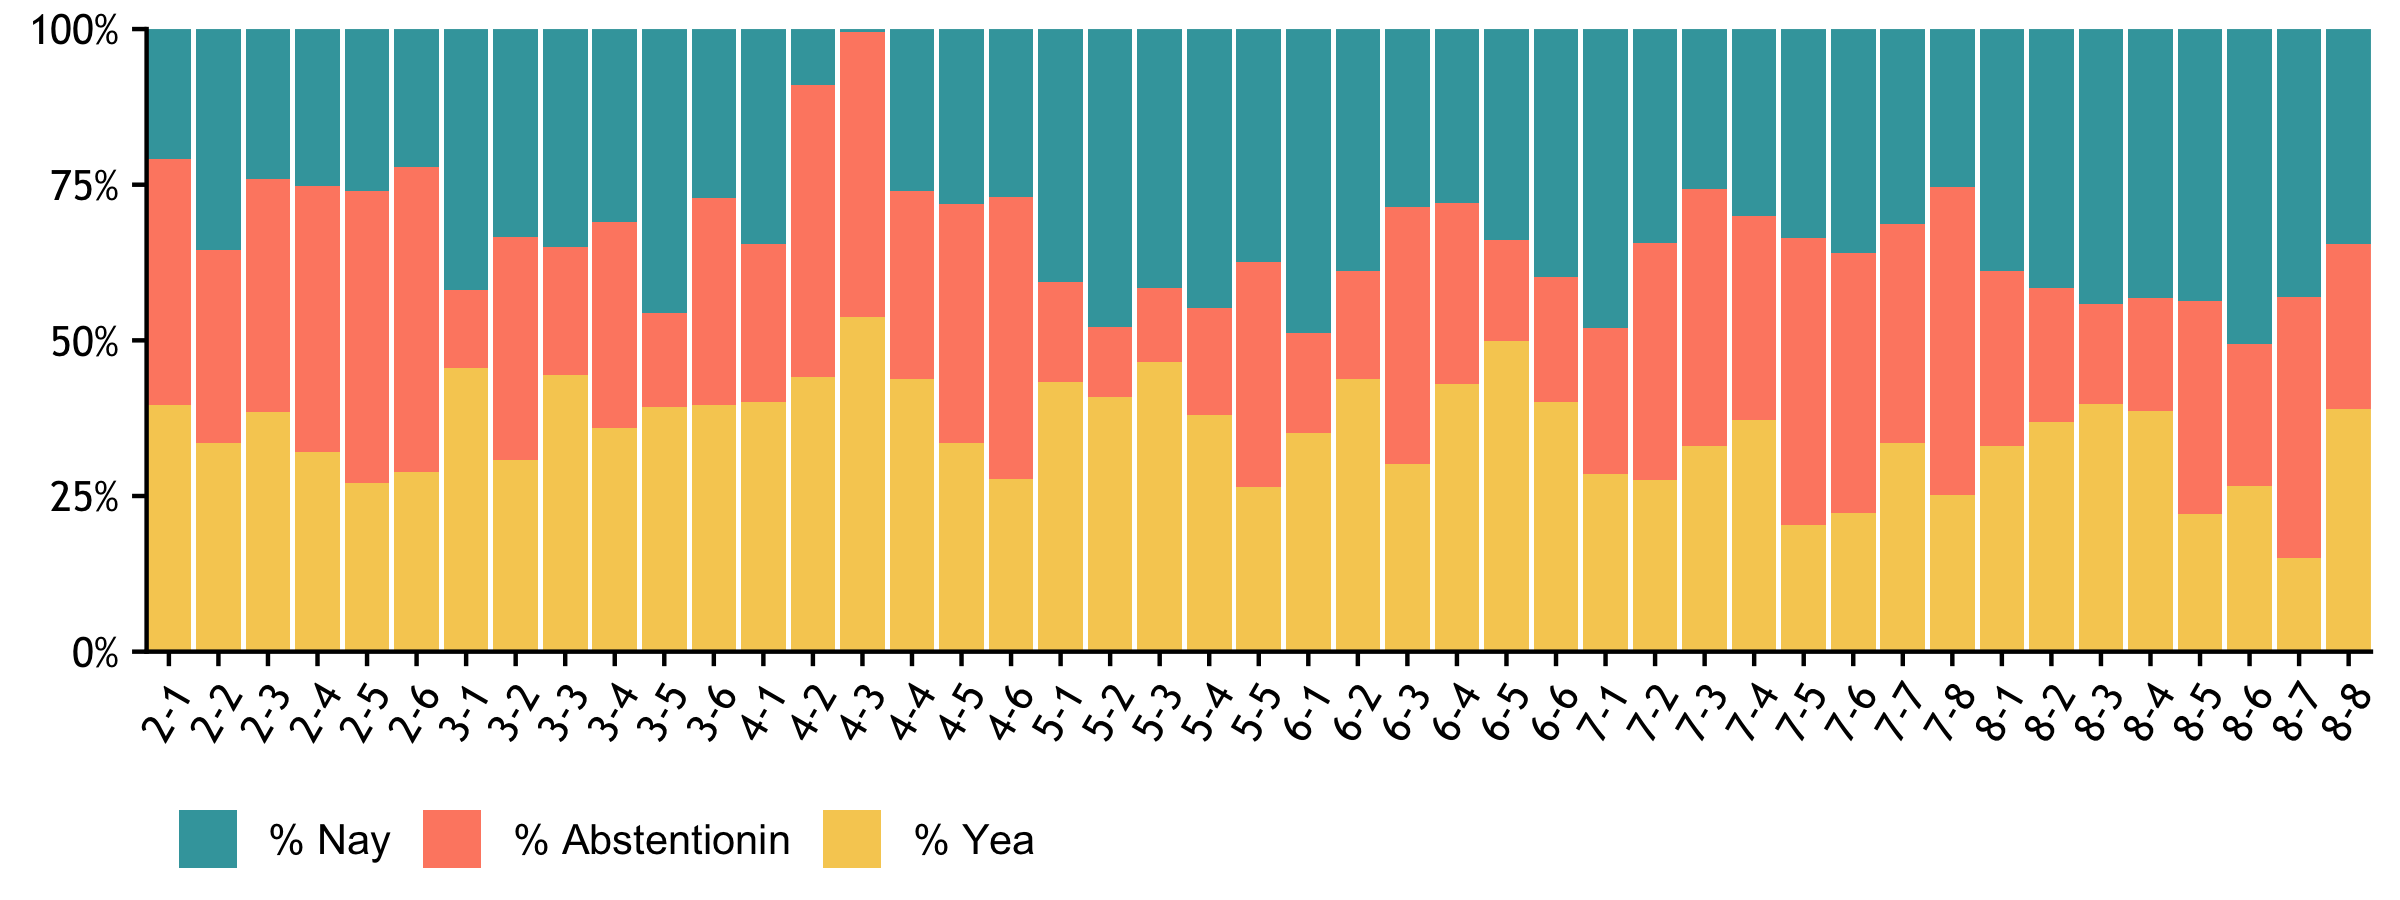
\includegraphics[width=14cm, height=6.8cm]{02-Chapter-Two/image/mean_rollcall.png}
    \caption{Proportions of Yea, Abstain  and Nay Votes \\ across Sessions}
    \label{fig:vote-distribution}
\end{figure}


\section*{\centering The Measurement of Legislator' Positions}


The spatial model of binary choice have revealed numerous insights into the structure and dynamics of legislative voting \citep[][]{Carroll2013,Clinton2004,Cox2002b, McCarty2001,McCarty2006,Snyder2001,Poole1997,Poole2007,Jackman2001,Tsai2020,Gray2019} and judicial preferences \citep[][]{Epstein2007,Martin2002,Martin2007}. In recent years, Item Response Theory based measure of legislative
voting developed by \textcite{Clinton2004} has been successful in
its application to understand legislative voting \citep[e.g.][]{Zucco2011, Tsai2020, Gray2019}. In its application, legislators as subjects possess a latent level of ability measured by varieties of roll calls and political ideology as ability. IRT measure can be utilised to set up item difficulty parameters to discover estimates of the voting preferences of legislators.

In particular, I estimate a separate ideological position for each legislator at the frequency of session. Parameters for bills are assumed
to be fixed across legislative sessions, so that I can estimate the positions of legislators over time. There are $N$ unique legislators
who voted bills and they are indexed by $i$, i.e. $i=1,2,...,N$. Let $J_{t}$ denote the total number of bills voted in the $t$th session, where $t$ does not exceed the total number of sessions, 40. For simplicity, denoted $j$ by the $j$th bill voted in the session $t$, where $j\leq J_{t}$. $i$ and $j$ record the location of the data in the dimension of legislators and bills, respectively. Therefore, the ``nay'' or ``yea'' vote by legislator $i$ for the $j$th bill in the session $t$ is denoted by $y_{ijt}$. If ``nay'' vote is recorded, $y_{ijt}=0$, and if ``yea'' vote is recorded, $y_{ijt}=1$. 

Given these notations, I can proceed to apply the Expectation-Maximization (EM) algorithm proposed by \citet{Imai2016} to estimate the dynamic ideal point model with binary outcomes. First, the single-dimension ideal point model is specified by

\begin{equation}
\begin{aligned}
Pr(y_{ijt}=1)=\Phi(\alpha_{jt}+\beta_{jt}x_{it})=\Phi(\tilde{x}_{it}\tilde{\beta}_{jt}^{T}),
\end{aligned}
\end{equation}

\noindent where $x_{it}$ is the $i$th legislator's ideal point at time session $t$, and $\alpha_{jt}$ and $\beta_{jt}$ represent the item difficulty and item discrimination parameters for the bill $j$ at session $t$. The second half of the equation expresses it into the vector form, where $\tilde{x}_{it}=(1,x_{it})$ and $\tilde{\beta}_{jt}=(\alpha_{jt},\beta_{jt})$. Further, the latent propensity $y_{ijt}^{*}$ is introduced, such that 

\begin{equation}
\begin{aligned}
{y_{ijt}^{*}=\tilde{x}_{it}\tilde{\beta}_{jt}^{T}+\zeta_{ijt},}
\end{aligned}
\end{equation}


\noindent where $\zeta_{ijt}\sim N(0,1)$ are $i.i.d$ shocks. The legislator $i$ ideal point process is specified through the following conditional (on prior) distribution:

\begin{equation}
\begin{aligned}
{x_{it}|x_{it-1}\sim N(x_{it-1},\sigma_{x}^{2}),}\label{eq:ideal-point}
\end{aligned}
\end{equation}

\noindent for $t=1,2,3,...,40$. In addition, I assume the initial prior for $t$ = 1 to be $x_{i0}\sim N(\mu,\Sigma_{x})$ for each legislator and choose the KMT party whip as the anchor subject. Note that different sets of legislators participated in different legislative sessions and in each session, different set of bills were voted. For legislators who abstained or were not in legislature at session $t-1$, the average ideological point within their party at session $t-1$, $\tilde{x}_{it}$, is used as their prior at session $t$. Ideological estimates are robust to different methods of generating missing priors.\footnote{For the estimation of ideal points, I use the \textbf{biIRT()} function from the\textbf{emIRT} package \citep[see][]{emIRT2021}. This function estimates a binary IRT model with two response categories, Yea and Nay. Subsequently, I use \textbf{makePriors()} function to generates diffuse priors as several matrices of starting values for the parameters, based on the number of legislators $N$, the number of bills $J$ and the number of a dimension $D$. That is, the parameters include prior means and covariance matrix for ideal points $x_{it}$ and $\alpha_{jt}$, $\beta_{jt}$, respectively. Note that the package currently supports estimation from one dimension, which means the number of the dimension $D$ is 1 (a single dimension). As for item difficulty $\alpha_{jt}$, item discrimination $\beta_{jt}$ and legislators' ideal points $x_{it}$, I use \textbf{getStarts()} function to generate the matrices of the parameters for first session.} 

Joint posterior distribution set up in this paper  is same as the equation (31) from \citet{Imai2016}. The estimation is conducted using the EM algorithms which consists of three steps as is described by equation (60)-(64) in their paper and discussed in \citet{Armstrong2020}. Moreover, \citet{Imai2016} found that the algorithm yields similar and comparable ideological estimates to the standard Markov chain Monte Carlo algorithm, but will process much faster and better with massive data. In this paper, I examine the impact of electoral reform in 2008 on within- and between-parties ideological dispersion. In fact, by using this model, where legislators form ideal points based on a Bayesian approach (process \autoref{eq:ideal-point}), I leave large room for inter-dependence and autocorrelation between ideal points. Later I show, despite of this setting, the occurrence of the electoral reform generates increased gaps between inter-party division and intraparty distance at the individual level. 

\subsection*{Ideal Point of Estimated Individual Legislators}

\autoref{fig:year-plot} plots estimated distributions of individual legislator's ideological positions clustered by parties for the two major parties (KMT and DPP) at a frequency of year from 1996 to 2015.\footnote{Appendix \ref{sec:Plots full} shows the estimated distributions for both parties at a frequency of session and all minority party a frequency of year. The top shaded area displays post-reform distributions and the bottom area illustrates pre-reform distributions of ideological positions.} Several patterns are illustrated from the figure. First, the distributions of DPP and KMT legislators' ideological positions started to shift to both poles when the reform occurred (year 2008), meaning that there was a drastic divergence in ideological positions between DPP and KMT legislators. This can be interpreted as a piece of evidence of inter-party political polarisation between DPP and KMT.\footnote{\autoref{fig:individual_point} in Appendix \autoref{sec:Plots full} shows individual legislator's positions grouped by year for both major parties (DPP and KMT).} Second, the distribution of ideological positions, particularly KMT, started to spread out across the spectrum after the reform, indicating that the intraparty ideological dispersion is exacerbated after the reform. Note that DPP tends to be ideologically cohesive across year, while KMT tend to be much more disperse, particularly in 2008 to 2010. This suggests that despite the unification of co-partisan legislators' position, different parties are witnessed to polarise their positions along the ideology spectrum. Moreover, the SMD demonstrates heterogeneous effects on two major parties. DPP become less polarised and its average ideology is neutralised, while KMT witnesses a further intraparty divergence in ideology, spreading across both ends of the spectrum.

\begin{figure}[ht]
\caption{Estimated Legislators' Ideological Positions for Major
Parties, Grouped by Party and Year \label{fig:year-plot}
}\centering{}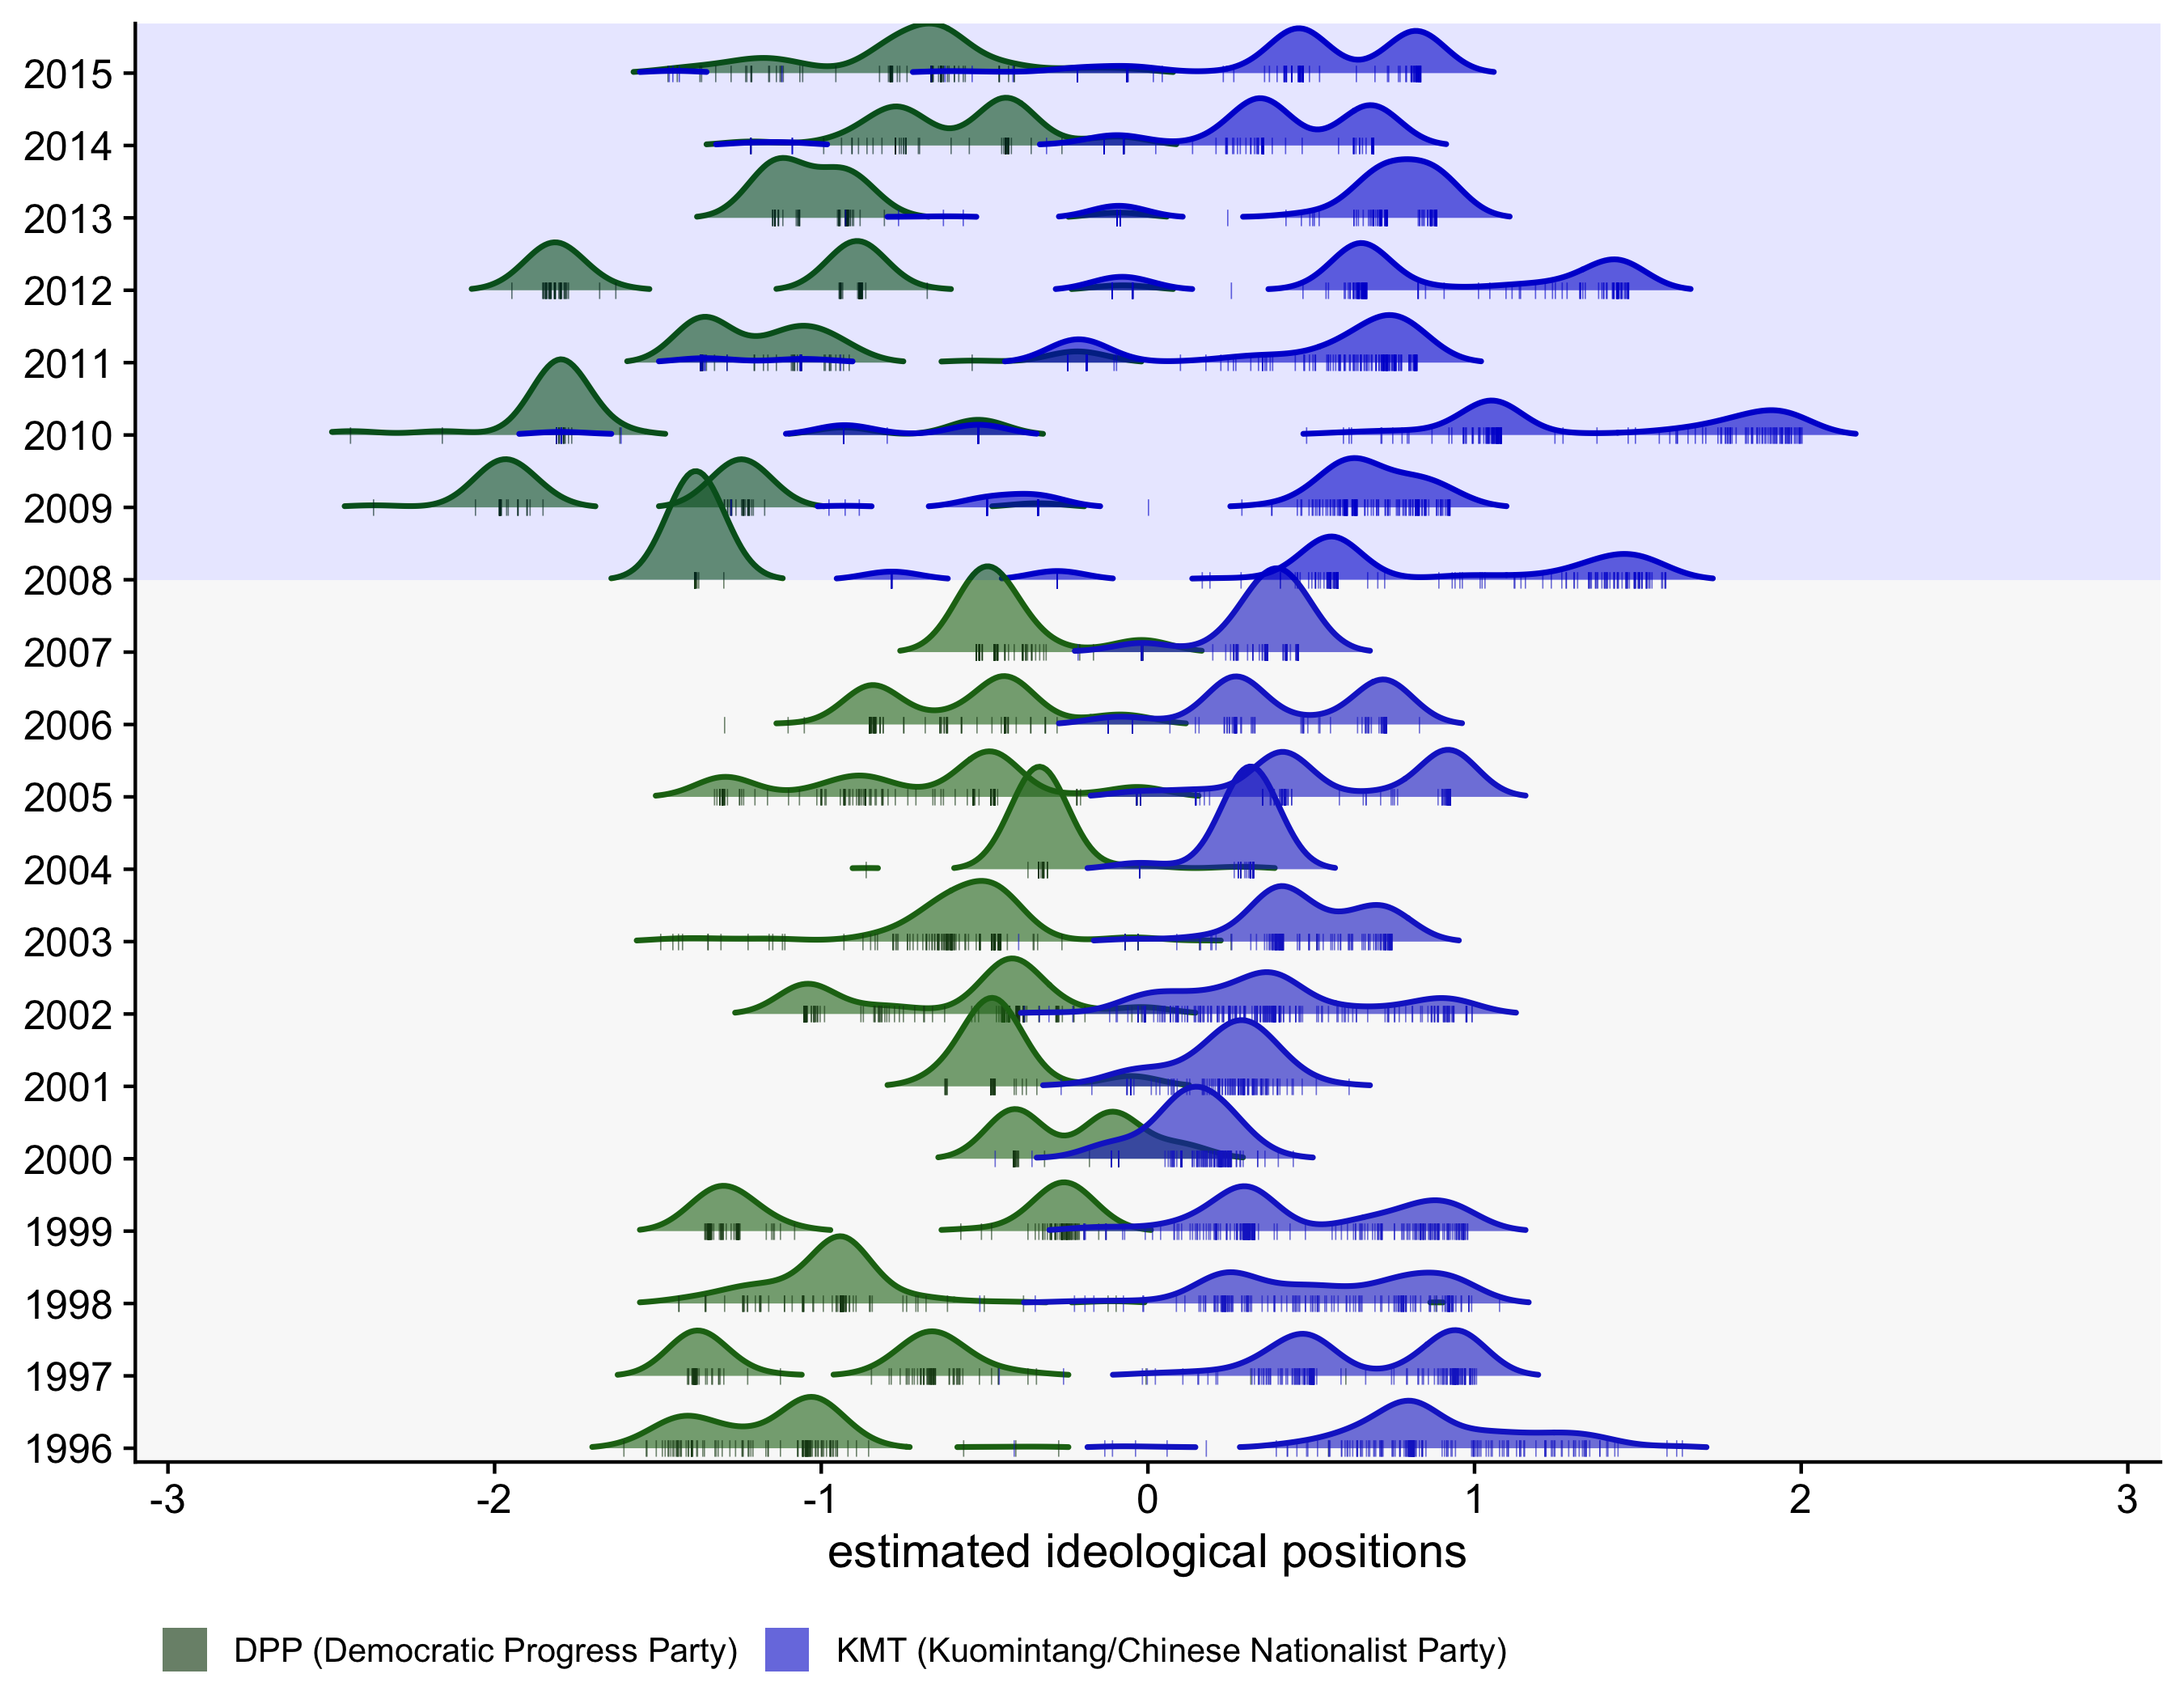
\includegraphics[scale=0.15]{02-Chapter-Two/image/major_postions_year.png}
\end{figure}

\subsection*{Party and Party Whip}

\begin{figure}[ht]
    \centering{}\caption{\label{Fig:2-1}
    Estimated Party Average and Party Whip's of Positions across Sessions \label{fig:whip_mean}}
    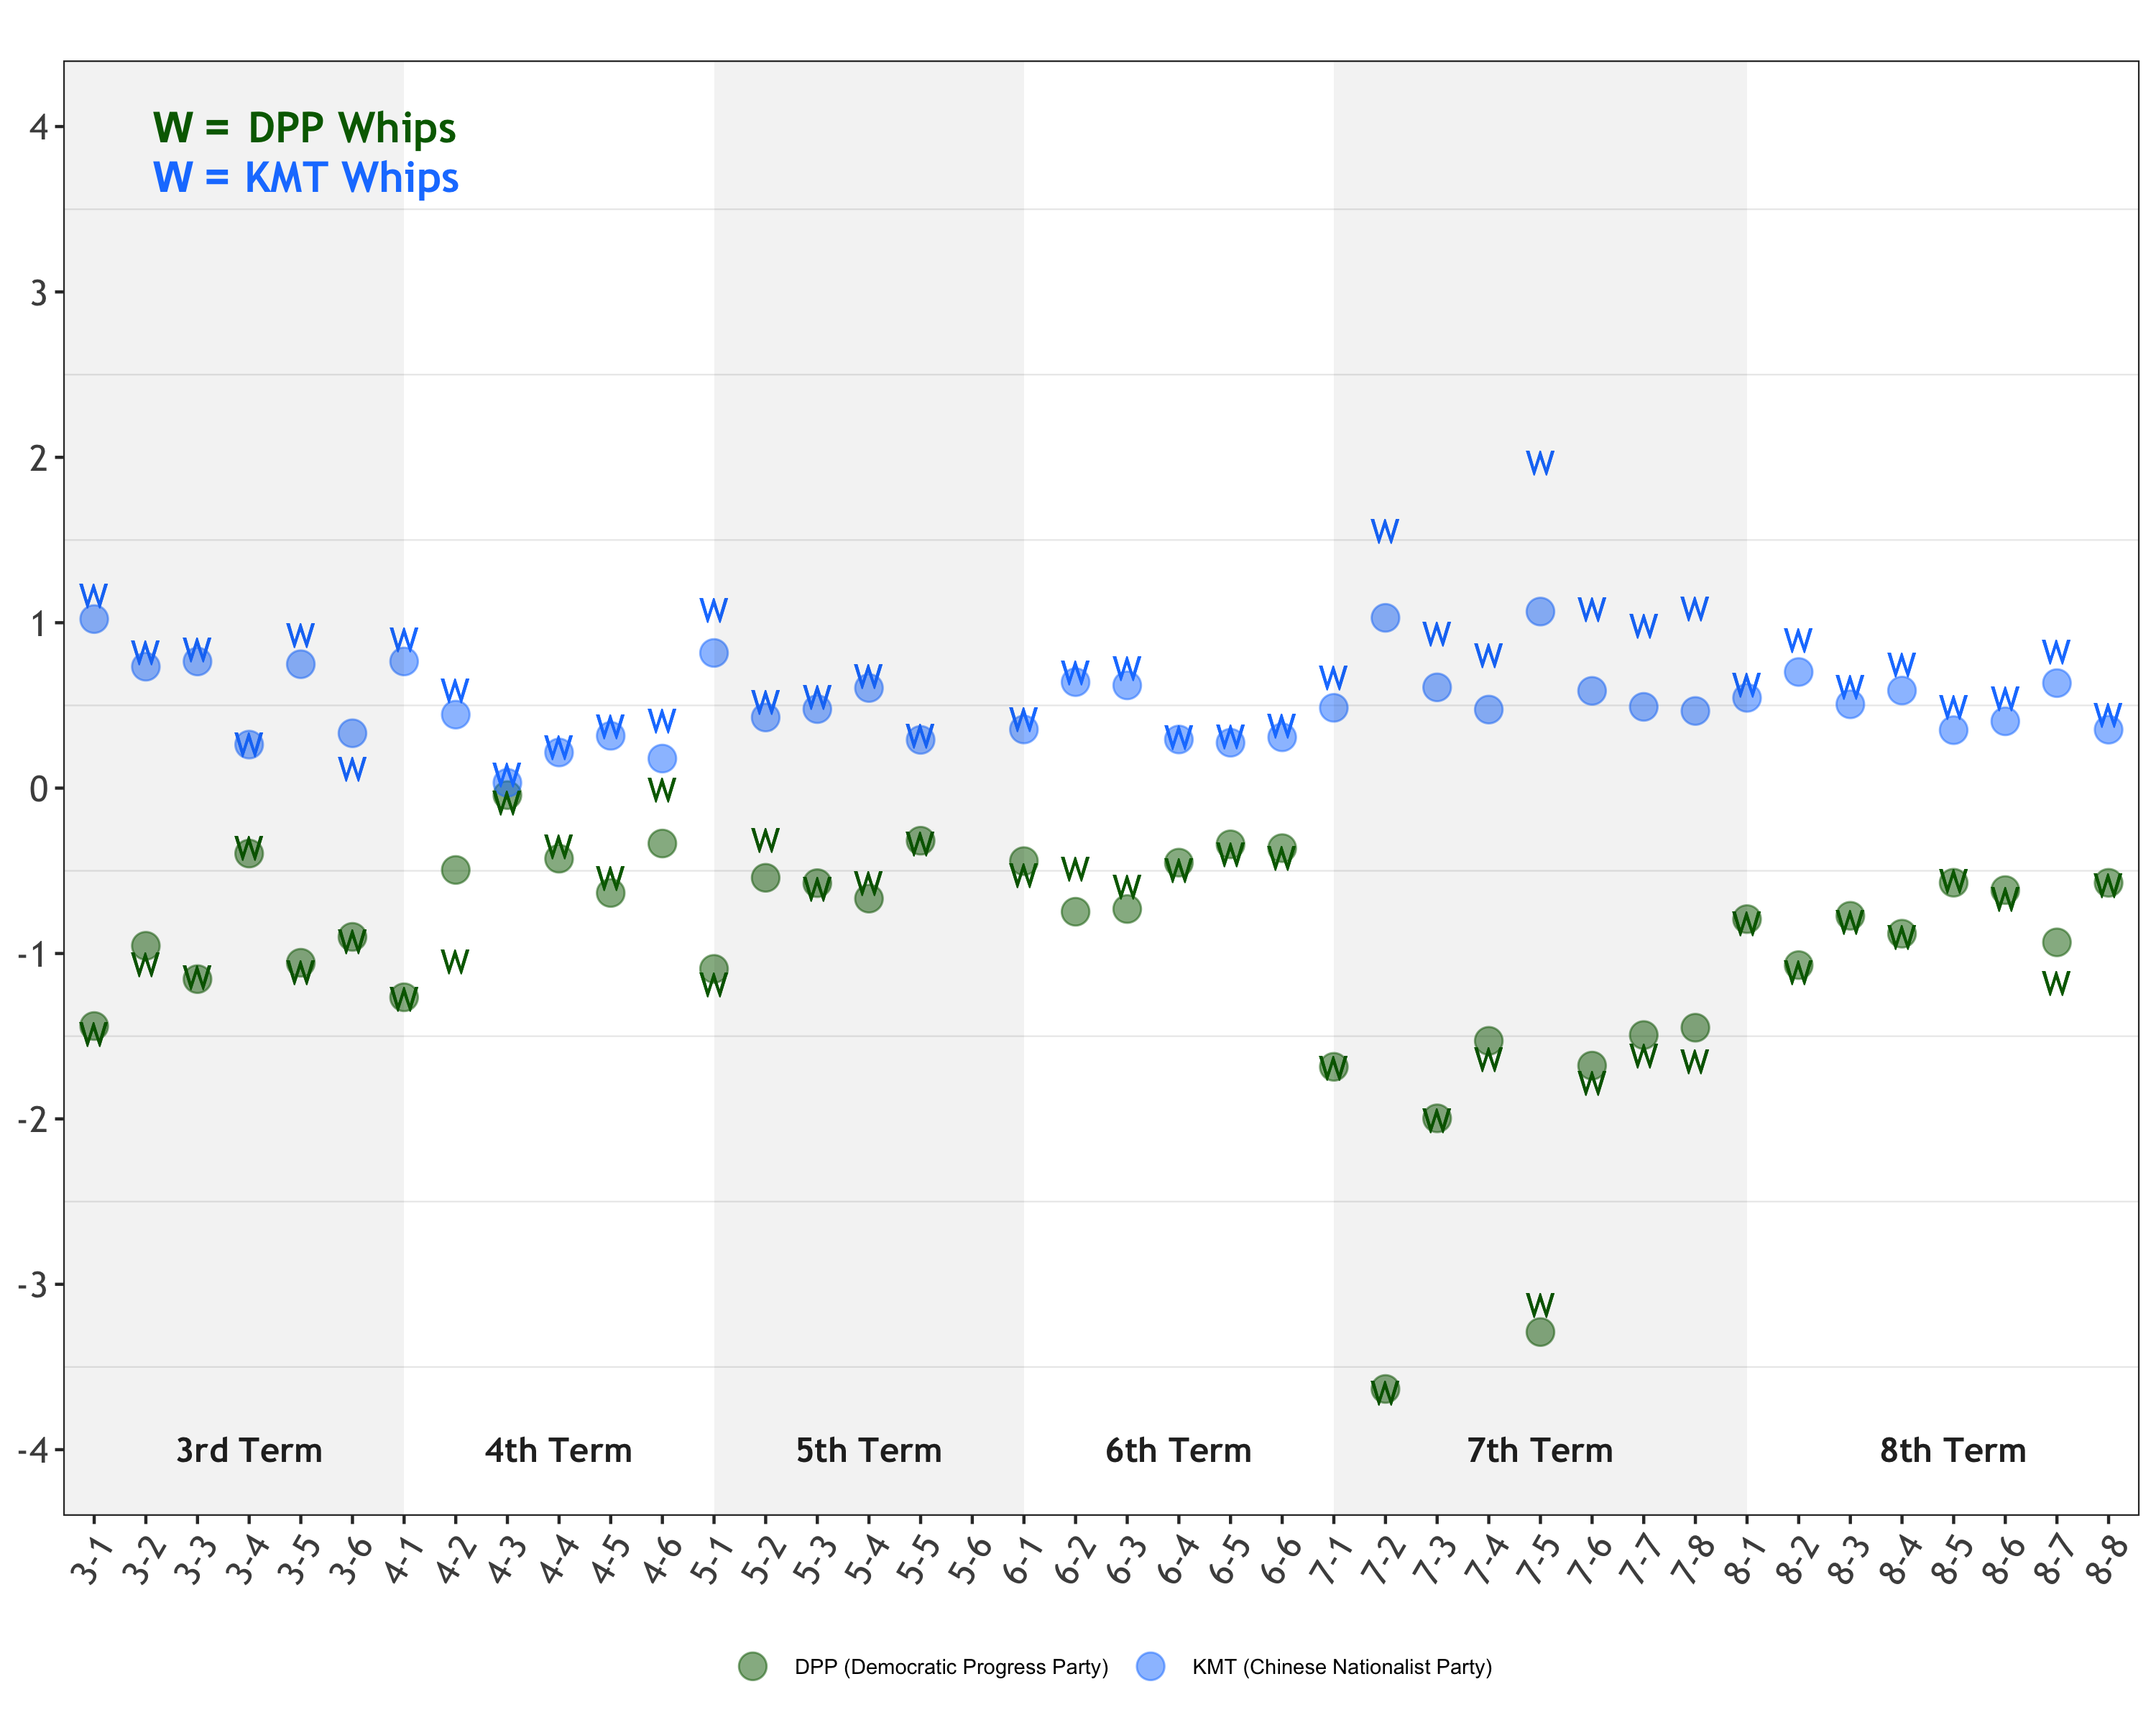
\includegraphics[width=14cm,height=9.5cm]{02-Chapter-Two/image/partywhip_mean}
\end{figure}

\autoref{fig:whip_mean} plots the estimated the average of party position and party whip's positions against sessions.\footnote{For KMT and DPP party whip's ideological positions are used to measure representative party positions, while for minor parties the average party ideological positions are used to measure representative party positions. This is due to the fact that in some sessions, party whips from some minor parties are not elected as legislators.} The figure displays the average estimated positions in each of the two major parties, KMT (denoted by ``blue dots'') and DPP (denoted by ``green dots''), while \textbf{\textit{W}} labels the party whip's positions for each party.\footnote{Apart from KMT and DPP, legislators from other minor parties are also included in the observation and used for regressions in column 1 and 2 in \autoref{tab:intra-estimation}.} \autoref{tab:Correlation} summarises some correlation statistics of the two major parties, DPP and KMT, showing that party average and party whip's ideological positions in the same party share a similar pattern (positive high correlation), while party average (or party whip's) ideological positions between KMT and DPP move in a quite opposite direction (negative high correlation). This implies the existence of political polarisation in terms roll call votes between KMT and DPP, and they are considered as rival parties.\footnote{Party whip plays an important role to ensure their co-partisans to vote policy position according to instructions made by their party central committee, rather than the will of their constituents. When voting for crucial bills or budget items, the whips may issue ``top-mobilisation order'' asking their legislators to attend voting sessions. Legislators disobeying the orders from party whips may be fined, suspended or even expelled from the party \citep{Hsu2002}.} 

Moreover, I specifically test in each party, if the average party voting behaviour seamlessly obeys the party's voting instruction (the whip's behaviour) across time using the following regression

\begin{equation}
whip_{it}=c_{i}+\phi_{i}\bar{party_{it}}+\zeta_{it}^{0},
\end{equation}

\noindent where $whip_{it}$ is the party $i$ whip's position, $\bar{party_{it}}$ is the corresponding party's average ideological position at session $t$, and $c_{i}$ is a constant. If the the average party voting behaviour follows the whip's voting behaviour, i.e. the the average obeys the party's instruction, constant $c_{i}=0$ and the coefficient $\phi_{i}=1$, simultaneously.

\begin{table}[ht]
\caption{Correlation Statistics of Estimated Position for Major Parties\label{tab:Correlation}}
\begin{centering}
\begin{tabular}{|c|cccc|}
\hline 
    \textbf{Correlation}                                & 
        $\overline{\textbf{party}}_{\textbf{KMT}}$          & 
        $\overline{\textbf{party}}_{\textbf{DPP}}$          &
        $\textbf{whip}\mathbf{_{KMT}}$                      &
        $\textbf{whip}\mathbf{_{DPP}}$                    \\
    \hline 
        $\overline{\textbf{party}}_{\textbf{KMT}}$          & 
        \done 1                                             &  
                                                            &  
                                                            & 
                                                            \tabularnewline
        $\overline{\textbf{party}}_{\textbf{DPP}}$          & 
        -0.702                                              & 
        \done 1                                             &
                                                            &
                                                            \tabularnewline
        {$\textbf{whip}\mathbf{_{KMT}}$}                    & 
         0.874                                              & 
        -0.881                                              & 
        \done 1                                             & 
                                                            \tabularnewline
        $\textbf{whip}\mathbf{_{DPP}}$                      & 
        -0.688                                              & 
        0.987                                               & 
        -0.870                                              & 
        \done 1                                             \tabularnewline
\hline 
\multicolumn{5}{l}{{$\overline{party}_\mathbf{i}$ denotes the average
position for party $i$, and $\mathbf{whip_{i}}$ }}         \tabularnewline
\multicolumn{5}{l}{{denotes the whip's position for party$i$, $i=KMT$ or $DPP$.}}                                                                         \tabularnewline
\end{tabular}
\par\end{centering}
\end{table}


Panel A in \autoref{tab:whip-position} reports regression outcomes for two major parties, individually. Panel B shows testing results using F test. As is illustrated in Panel B, I fail to reject the null of obedience to party instruction for DPP, while I reject the null for KMT, indicating the average DPP party voting behaviour seamlessly obeys whip's behaviour and KMT otherwise. Moreover, above test outcomes also justify when proceeding to test \textbf{Hypotheses \ref{h:p1-h1}} and \textbf{\ref{h:p1-h2}} respectively, I calculate inter- and intraparty ideological dispersion for both KMT and DPP respectively using the ideological differences between individual legislators and the corresponding party whip, due to this discrepancy in whip's position and average party position.


\begin{table}[tp]
\caption{Testing for the Obedience of Legislators' Voting Behavior
to Instruction Issued by Party Whip
\label{tab:whip-position}}

\centering{}%
\begin{tabular}{lcc}
\toprule 
 & \textbf{DPP} & \textbf{KMT}\tabularnewline
\midrule 
\multicolumn{3}{l}{\textbf{Panel A: regression results}}\tabularnewline
\multicolumn{3}{l}{\textbf{Dependent variable: }whip's position}\tabularnewline
\midrule 

\textbf{average party position} & {1.000$^{***}$} & {1.304$^{***}$}\tabularnewline
 & (0.027) & (0.119)\tabularnewline
\textbf{constant} & -0.023 & 0.023\tabularnewline
 & (0.033) & (0.068)\tabularnewline
\textbf{No. of observations} & 39 & 39\tabularnewline
\textbf{Adjusted \textit{R}$^{2}$} & 0.97 & 0.76\tabularnewline
\textbf{Prob > F} & 0.00 & 0.00\tabularnewline
\midrule
\multicolumn{3}{l}{\textbf{Panel B: testing outcomes}}\tabularnewline
\midrule
\multicolumn{3}{l}{\textbf{$\mathbf{H_{0}}$}:\textbf{ $c_{i}=0$ }and\textbf{ $\phi_{i}=1$}}\tabularnewline
\textbf{Prob > F} & 0.307 & 0.000\tabularnewline
\textbf{Reject $H_{0}$} & No & Yes\tabularnewline
\midrule
\multicolumn{3}{l}{{Asterisk indicates significant level: {*}: p < 0.10;
{*}{*}:}}\tabularnewline
\multicolumn{3}{l}{{p < 0.05; {*}{*}{*}:p < 0.01.}}\tabularnewline
\end{tabular}
\end{table}


\section*{\centering Empirical Findings}

I merge validated estimates of legislators' ideological positions across sessions with legislator profiles and election data from the database of the Taiwanese Legislative Yuan (Congress Research Services), and perform statistical tests below.

\subsection*{Interparty Polarisation\label{subsec:political-polarization}}

To evaluate the \textbf{Hypothesis \ref{h:p1-h1}}, I calculate the legislator-level inter-party dispersion between two major parties, KMT and DPP (between party polarisation). The inter-party dispersion is defined as the distance of ideological positions between individual legislator and the opponent party whip in each legislative session, \boldsymbol{$interdistance_{it}$}. It is calculated as: 

\begin{equation}
\mathbf{interdistance_{it}=|position_{it}-\bar{whip_{it}|}},
\end{equation}

\noindent where $position_{it}$ denotes the ideological position of legislator $i$ at session $t$ and $\bar{whip_{it}}$ denotes the ideological position of the opponent party whip for legislator $i$ at time $t$. For instance, if legislator $i$ is affiliated to KMT (DPP), then $interdistance_{it}$ is the ideological distance between his estimated position and DPP (KMT) whip's estimated position, at session $t$.

Following \citet{Catalinac2017}, I specify the following regression model, allowing the passage of time (year) to have different marginal effects on inter-party ideological distance, prior to and post the electoral reform.

\begin{align}
\mathbf{interdistance_{it}=\alpha_{0}+\alpha_{1}electoralreform_{t}+\alpha_{2}year_{t}+}\nonumber \\
\mathbf{\alpha_{3}(year_{t}\times electoralreform_{t})+C_{it}+\epsilon_{it}^{1},}\label{eq:interdistance}
\end{align}

\noindent where $year_{t}$ is the year dummy indicating in which year the session $t=1,2,...,39$ (pertaining the 1st, the 2nd, the 3rd,..., the 39th session in our observation, respectively) is held.\footnote{Total 39 sessions is due to the lack of data for the 5-6 session in year 2005.} $electoralreform_{t}$ is a dummy variable showing whether an observation belongs to the post-transition phase (i.e. if $t\geq24$) if $electoralreform_{t}=1$. $C_{it}$ contains controls pertaining to legislator $i$ and in session $t$: legislator attributes, party-affiliation dummies, and electoral district attributes. Specifically, legislator attributes include each legislator's sex and marginal winning share. Marginal winning share is defined as the excessive percentage points of votes the legislator won comparing to the legislator who won the next most votes. Party-affiliation dummy here is denoted by $KMT$. If the legislator $i$is affiliated to KMT, $KMT=1$; otherwise, $KMT=0$. Electoral district attributes control for the size of each electoral district: if a district's magnitude is over 9, $bigdistrict=1$ and $middistrict=0$; if its magnitude is between 5 to 8, $bigdistrict=0$ and $middistrict=1$; if its magnitude is below 5, $bigdistrict=0$ and $middistrict=0$. And the standard assumptions of homoskedasticity apply to the error term $\epsilon_{it}^{1}$.

\begin{table}[ht]
\caption{Interparty Ideological Differences\label{tab:inter-estimation}}

\centering{}%
\scalebox{0.95}{
\begin{tabular}{lcc}
\toprule 
\multicolumn{3}{l}{\textbf{Dependent variable:}}\tabularnewline
\multicolumn{3}{l}{Interparty Ideological Differences between Mainstream Parties}\tabularnewline
\midrule
 & \textbf{interaction} & \textbf{(+ controls)}\tabularnewline
\midrule
\textbf{electoral reform} & 16.21{9$^{***}$} & 15.291{$^{***}$}\tabularnewline
 & (0.747) & (0.867)\tabularnewline
\textbf{year} & {-0.242$^{***}$} & -0.238{$^{***}$}\tabularnewline
 & (0.008) & (0.010)\tabularnewline
\textbf{year }\textbf{$\times$ electoral reform} & -0.643{$^{***}$} & {-0.599$^{***}$}\tabularnewline
 & (0.040) & (0.046)\tabularnewline
\textbf{marginal winning shares} &  & 0.026\tabularnewline
 &  & (0.202)\tabularnewline
\textbf{intercept} & 3.40{5$^{***}$} & 3.697{$^{***}$}\tabularnewline
 & (0.071) & (0.252)\tabularnewline
\textbf{legislator attributes} &  & $\checkmark$\tabularnewline
\textbf{party dummies} &  & $\checkmark$\tabularnewline
\textbf{district fixed effects} &  & $\checkmark$\tabularnewline
\midrule
\textbf{No. of observations} & 5663 & 4170\tabularnewline
\textbf{Adjusted \textit{R}$^{2}$} & 0.28 & 0.27\tabularnewline
\textbf{Prob > F} & 0.00 & 0.00\tabularnewline
\midrule
\multicolumn{3}{l}{{Robust standard errors are reported in parentheses. Asterisk indicates}}\tabularnewline
\multicolumn{3}{l}{{significant level: {*}: p < 0.10;
{*}{*}: p < 0.05; {*}{*}{*}:p < 0.01.}}\tabularnewline
\end{tabular}}
\end{table}

\autoref{tab:inter-estimation} reports the estimation results, where the dependent variable is legislator's inter-party ideological distance. Both \textbf{electoral reform} and \textbf{year $\times$ electoral reform }are statistically significant, with (column 2) or without incorporating controls (column 1). Specifically, the coefficient on \textbf{electoral reform} is statistically significant (at 1\% critical level) in both cases, suggesting electoral reform had a significant positive impact on the inter-party ideological distance between the two major parties (KMT and DPP), even when the passage of time (year) and other legislator-, party- and district-level attributes are controlled for. After the reform, a typical legislators from KMT (DPP) underwent a phase of polarisation in terms of the roll call votes, i.e. her ideological positions became further away from the DPP (KMT). Therefore, the estimation rejects the \textbf{Hypothesis \ref{h:p1-h1}} and the electoral reform significantly polarised legislators from the rival party. \autoref{fig:inter-fitted} plots the fitted value of legislator-level inter-party ideological distance with their 95\% confidence intervals against year. At 2008 (when the reform occurred), there was a drastic leap in between-party ideological distance. The significance of the coefficient on the interaction term \textbf{year $\times$ electoral reform} implies that the passage of time (year) indeed had heterogeneous effect on between-party distance. It also shows that the increase in time resulted in lower-level distance.\footnote{To ensure these results are not driven by any individual major party, Appendix \ref{sec:robustness-check} reports the estimation results separately for the two major parties and finds the robustness of the results.} 

\begin{figure}[ht]
\caption{Fitted Values of Inter-party Ideological Distance between KMT and DPP with 95\% Confidence Intervals \label{fig:inter-fitted}}\centering{}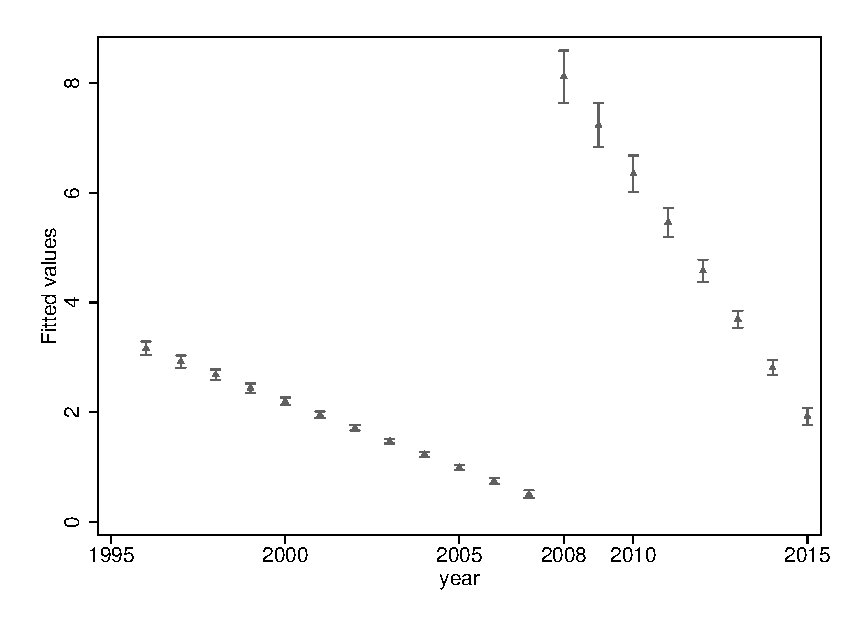
\includegraphics[scale=0.59]{02-Chapter-Two/image/all_inter.eps}
\end{figure}

\autoref{fig:individual_legislators} shows seven most senior legislators and individual legislators' ideal points for two major parties, KMT (denoted by ``K'') and DPP (denoted by ``D''). As illustrated in \autoref{fig:individual_legislators}, two major parties diverge drastically after the introduction of SMD in the 7th session. Note that the ideological positions of the seven most senior legislators, including five KMT and three DPP legislators, who have served in the Legislative Yuan over twenty years, are highlighted and aligned individually in the figure. It clearly demonstrates how the electoral reform in 2008 changes their positions: senior legislators from KMT and DPP tend to be more spatially converged under the SNTV system, whereas both parties appear to diverge against each other under the SMD, also consistent with our empirical findings.

\begin{figure}[ht]
\caption{Ideal Point of Individual Legislator \label{fig:individual_legislators}}\centering{}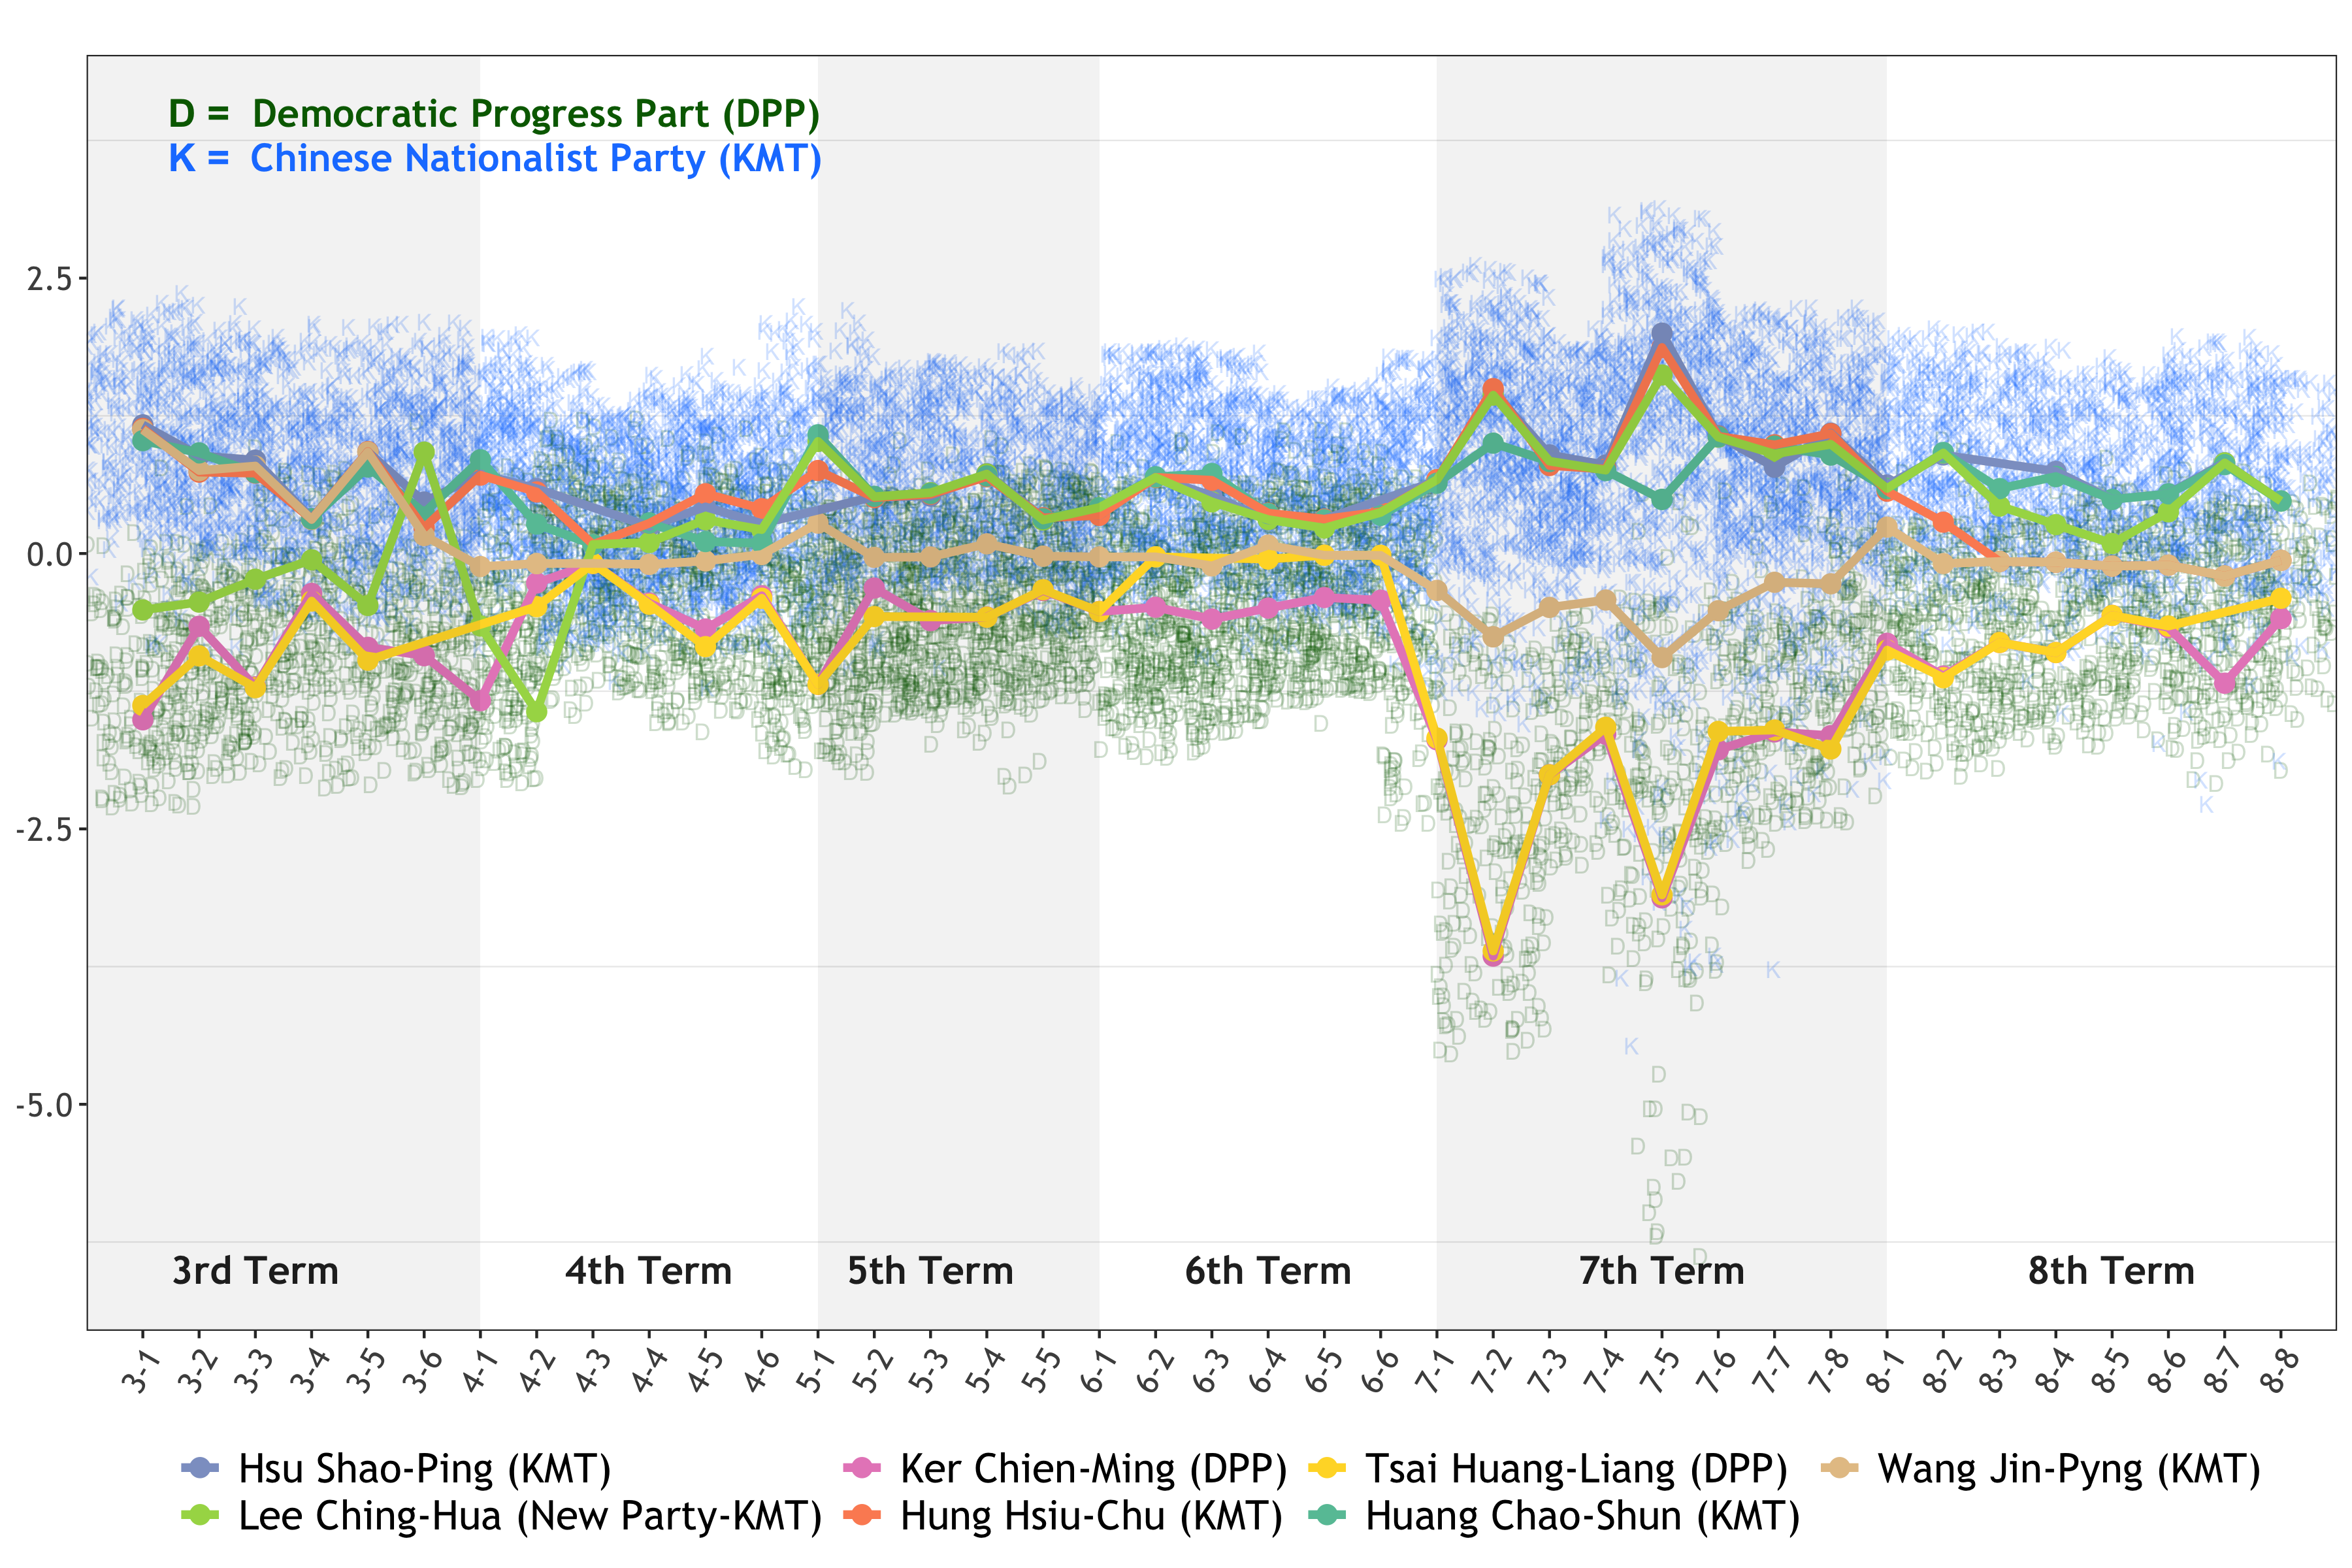
\includegraphics[width=13cm, height=9.5cm]{02-Chapter-Two/image/seven_legis}
\end{figure}

\citet{Catalinac2017} illustrates the robustness using sub-sample only including competitive candidates. In our regression, I include \textbf{marginal winning share} of each legislator in each legislative session as a control, which implies the competitiveness of the corresponding legislator. As it is not statistically significant (p > 0.10), it suggests that our estimation results are robust to using competitive legislators as the sample. Also, some are concerned that the inter-party dispersion were caused by the heterogeneity in bills voted across time, i.e. in some years, controversial bills (which are more likely to cause inter-party dispersion) are voted. To show that the inter-party dispersion before and after the reform was not caused by such heterogeneity, Appendix \ref{sec:robustness-check} addresses this problem by controlling for as many year dummies as possible and finds the robustness of our results.


\subsection*{Disunity in Co-partisan Legislators after the Reform\label{subsec:disunity-in-co-partisan}}

To evaluate \textbf{the Hypothesis \ref{h:p1-h2}}, I calculate the dispersion in co-partisan legislator's estimated ideological positions (within-party disunity). The dispersion here is defined as the distance between individual legislator's ideological positions and the co-partisan whip in each legislative session, $intradistance_{it}$. It is calculated as: 

\begin{equation}
\mathbf{intradistance_{it}=|position_{it}-whip_{it}|,}
\end{equation}

\noindent where $position_{it}$ denotes the ideological position of legislator $i$ at session $t$ and $whip_{it}$ denotes the ideological position of the party whip for legislator $i$ at session $t$. The regression model is constructed as follow.

\begin{align}
\mathbf{intradistance_{it}=\beta_{0}+\beta_{1}electoralreform_{t}+\beta_{2}year_{t}+ \nonumber } \\
\mathbf{\beta_{3}(year_{t}\times electoralreform_{t})+\tilde{C}_{it}+\epsilon_{it}^{2},\label{eq:intradistance}}
\end{align}

\noindent where $\tilde{C}_{it}$ contains controls. The only difference between $C_{it}$ in model (\autoref{eq:interdistance}) and $\tilde{C}_{it}$ is that more party-affiliation dummies are included in the controls. The rest estimation strategy are same as previously defined in the model (\autoref{eq:interdistance}).

\begin{table}[h]
\caption{Intraparty Distance at the Sessional Level\label{tab:intra-estimation}}
\centering{}%
\scalebox{0.85}{
\begin{tabular}{lccccc}
\toprule 
\multicolumn{6}{l}{\textbf{Dependent variable:} } \\
\multicolumn{6}{l}{Intraparty Ideological Distances} \\
\midrule 
                                                 & 
        \multicolumn{2}{c}{\textbf{All parties}} &  
                                                 & 
        \multicolumn{2}{c}{\textbf{Major parties}} \tabularnewline
        \cmidrule{2-3} \cmidrule{5-6}
                                                 & 
        \textbf{interaction}                     & 
        \textbf{(+ controls)}                    &  
                                                 & 
        \textbf{interaction}                     & 
        \textbf{(+ controls)}                       \tabularnewline
\midrule

\textbf{electoral reform}   & 1.79{1$^{***}$}   & 2.375{$^{***}$}   &          & {1.823$^{***}$} & {2.464$^{***}$}  \\
                            & (0.255)           & (0.336)           &          & (0.263)         & (0.199)          \\
\textbf{year}               & -0.0{04$^{***}$}  & -0.0{03$^{**}$}   &          & -0{.003$^{***}$}& {-0.004$^{**}$}  \\
                            & (0.001)           & (0.002)           &          & (0.001)         & (0.002)          \\
\textbf{year$\times$ electoral reform}  & -0.{082$^{***}$} & {-0.114$^{***}$} &         & {-0.083$^{***}$} & -0.11{7$^{***}$} \\
                                        & (0.013)          & (0.017)          &         & (0.013)          & (0.018)\\
\textbf{marginal winning shares}        &                  & -0.121           &         &                  & 0.041\\
                                        &                  & (0.269)          &         &                  & (0.084)\\
\textbf{intercept}                      & 0.0{80$^{***}$}  & -0.125{$^{*}$}   &         & 0.07{8$^{***}$} & -0.142{$^{*}$}\\
                                        & (0.006)          & (0.073)          &         & (0.009)         & (0.083)\\
\textbf{legislator attributes}          &                  & $\checkmark$     &         &                 & $\checkmark$\\
\textbf{party dummies}                  &                  & $\checkmark$     &         &                 & $\checkmark$\\
\textbf{district fixed effects}         &                  & $\checkmark$     &         &                 & $\checkmark$\\
\midrule
\textbf{No. of observations}            & 6736             & 4969             &         & 5663            & 4170\\
\textbf{Adjusted R$^{2}$}               & 0.04             & 0.05             &         & 0.04            & 0.05\\
\textbf{Prob > F} & 0.00 & 0.00 &  & 0.00 & 0.00\\
\midrule
\multicolumn{6}{l}{{Robust standard errors are reported in parentheses. Asterisk indicates significant }}\tabularnewline
\multicolumn{6}{l}{{level: {*}: p < 0.10;
{*}{*}: p < 0.05; {*}{*}{*}:p < 0.01.}}\tabularnewline
\end{tabular}}
\end{table}

\autoref{tab:intra-estimation} reports the estimation results, where the dependent variable is legislator's within-party ideological
distance. Column 1 and 2 illustrate outcomes using observations from all parties with or without controls. The variable of \textbf{electoral reform} had
statistically significant positive (at 1\% critical level) impact on co-partisan ideological distance, even when I control for the passage
of time (year) and other legislator, party, and district attributes. After the reform, legislators became more distant from co-partisan
whips (i.e. more disunited) in terms of ideological positions. Therefore, I reject the \textbf{Hypothesis \ref{h:p1-h2}} and the electoral reform significantly dis-united co-partisan legislators. Although this finding is contrary to manifesto studies like \citet{Catalinac2017} that candidates position themselves more cohesively with other co-partisan candidates in single-member districts, it is generally complementary with study of \citet{Jang2019}'s seminar work on Taiwan legislative roll call of the entire period of the SNTV-MMD system, which argues that legislators have varying degree of personal vote incentives when they face different electoral challenges. 

\begin{figure}[ht]
\caption{Fitted Values of Intraparty Ideological Distances in 95\% Confidence Intervals \label{fig:intra-fitted}}
\centering{}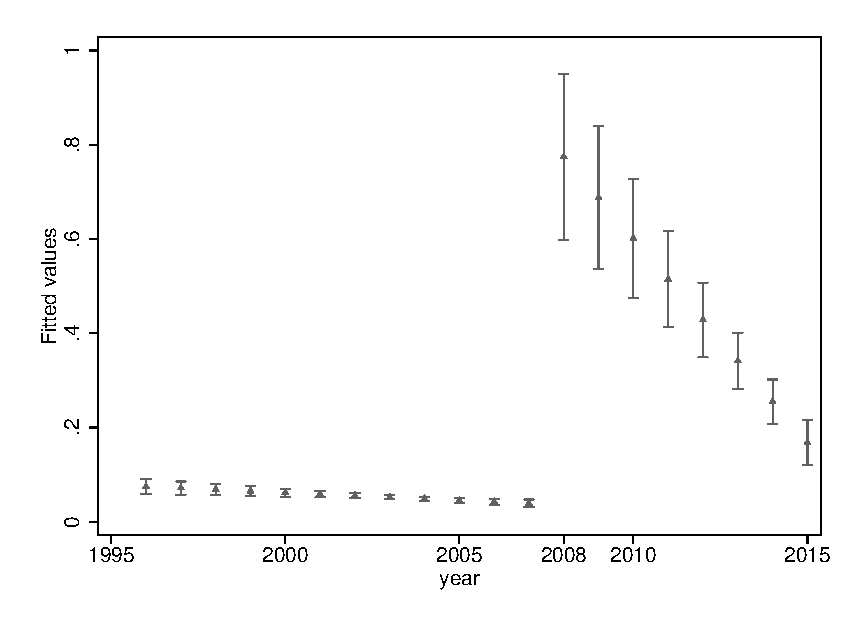
\includegraphics[scale=0.59]{02-Chapter-Two/image/KD_intra}
\end{figure}

The left-hand side in \autoref{fig:intra-fitted} plots the fitted value of intraparty ideological distance with their 95\% confidence intervals against year using the sample of legislators form all parties. At the 2008 (when the reform occurred), there was a leap in within-party ideological distance. Since the intersection term \textbf{year $\times$ electoral reform }is significant, time had heterogeneous effect on co-partisan ideological distance, before and after the reform. The outcomes also suggest that the increase in time was accompanies by lower levels of within-party distance. Column 3 and 4 show that the estimation is robust to using different sample of legislators (from the two major parties, KMT and DPP), with or without controls, respectively. The fitted value for this estimation is plotted at right-hand side in \autoref{fig:intra-fitted}. Moreover, since the control variable \textbf{marginal winning shares }is statistically insignificant, regression outcomes are also robust to use competitive legislators as the sample. To ensure these results are not driven by any individual major party, Appendix \ref{subsec:disunity-robust} reports the estimation results separately for the two major parties and finds the robustness of the results.

\section*{\centering Conclusion and Discussion}

This paper looks at a long-lasting myth of the impact of 2008 Taiwan electoral reforms. Although Taiwan transformed from SNTV to SMD, as scholars argue, some evidence indicates that SMD may not be as effective as originally thought in solving drawbacks of SNTV, such as polarized parties. Recently, conflicts between the two major parties
intensify and with-in party relationship becomes growingly rigid and tense. This project is a pioneer in empirically and formally testing the polarization and conflicts in legislator's attitude, prior and post the election reform using individual-level ideological positions extrapolated from legislative roll calls, adding contribution to a deeper understanding of potential impact of the reform on partisan relationship. 

Particularly, two hypotheses regarding the legislators' ideological positions are tested:1) switching from SNTV to SMD mitigated the level of political polarization between parties, particularly between
KMT and DPP; 2) switching from SNTV to SMD united co-partisan legislators in terms of ideological positions. Our findings suggest a phase of ``disunited polarization'' among inter-party and co-partisan legislators during the transition. Empirical test results show that this switching not only exacerbated inter-party ideological polarization by distancing legislators' positions from their opponents, but also disunited co-partisan legislators as their positions became more widely distributed along the ideological spectrum. These outcomes are robust to including various sets of controls and different samples of parties, and without or with controlling the heterogeneity in the nature of bills voted across time.

Although the first finding is contrary to some manifesto studies like \citet{Catalinac2017} that SMD reduce the inter- and intraparty polarization in countries like Japan, it is complementary with the study of \citet{Jang2019}'s seminar work on Taiwan legislative roll calls over the entire period of the SNTV-MMD system. The discrepancy between Taiwan and Japan results could possibly be attributed to the
multi-cultural environment in Taiwan. Our paper contributes to the large body of literature of electoral reforms by adding some empirical evidence in Asian democracies and also it highlights the possibility of the ineffectiveness of using electoral reforms as means of alleviating political chaos. 
%%%%%%%%%%%%%%%%%%%%%%%%%%%%%%%%%%%%%%%%%%%%%%%%%%%%%%%%%%%%%%
%%                This is Chapter 3 (Paper 3)               %% 
%%%%%%%%%%%%%%%%%%%%%%%%%%%%%%%%%%%%%%%%%%%%%%%%%%%%%%%%%%%%%%
\chapter{Electoral Reform and Pork Barrel in Parliamentary Questions  \label{chap:ch3}  }
\clearpage

\section*{\centering Abstract}
\small Measuring legislator behaviours and tendencies towards constituencies under different electoral systems is important. This chapter quantitatively investigates this topic using the case of Taiwan Legislative Yuan and data on written parliamentary questions through an electoral reform from multi-member districts (MMD) to single-member districts (SMD). With existing labelled pork legislation, I train deep learning models using convolutional neural networks with an embedding layer extracted from Transformer BERT to detect pork-barrel features in parliamentary questions over time. Evidence exists to show that legislators under MMD are more likely to express political intentions regarding pork-barrel projects in written parliamentary questions. The institutional change subsequently demonstrates heterogeneous effects on large parties vis-à-vis small parties.\footnote{I wish to thank Julia Park, Akitaka Matsuo, Royce Carroll, Lawrence Ezrow, Sven-Oliver Proksch, Christine Sylvester, Chris Arnold, Melanie Goodrich, Yaoyao Dai, Walter Mebane, Alexander Kustov and the participants at ESSEX-HEROEs, 2022 COMPTEXT, 2022 PolMeth for invaluable discussion and comments on previous versions of this paper. I also gratefully acknowledge using Prof.I also gratefully acknowledge using Prof. Dr Ching Jyuhn Luor (羅清俊教授)'s collection of digitized pork-barrel legislation and the High-Performance Computing Facility (CERES) at the University of Essex. }  

\clearpage

\section*{\centering Introduction}
How does the electoral reform change legislators' preference and their intentions to bring home the bacon? Scholars have clearly explained why intraparty competition by different rules of electoral systems increases legislators' incentives to run on a personal reputation \citep{Cox1990, Downs1957, Carey1995}. For example, candidates under multi-member districts (MMD) are more likely to reward small groups of supporters with particularised benefits and deviate from their party line, whereas candidates under single-member districts (SMD) prefer to adopt electoral strategies that target median voters \citep{Cox1990}. With abundant literature on an empirical examination of the relationship between electoral systems and political behaviours \citep[e.g.][]{Cox1990, Catalinac2016, Catalinac2017, Goplerud2021}, we however know little about whether actual impacts introduced by the electoral reform through MMD to SMD reduce legislators' motives to purse pork barrel project in the legislature. Understanding such legislative motions is very important for the process of policy making and decision. 

Parliamentary activities such as debates and written parliamentary questions, play a significant role in most parliamentary democracies. For example, the floor debate functions as a major platform for Members of Parliament (MPs) to uncover information and discussion regarding government policy, proposed new laws and topical issues of the day. With different regulations limiting MPs to access to the floor, the distribution of time and topics tends to be restricted to displace salient issues \citep[e.g., ][]{Back2019b, Martin2011}, which increase difficulties in discovering MPs' genuine interests in preferences \citep{Martin2011, Saalfeld2011, Russo2021} and their nature of substantive representation \citep{Kolpinskaya2017}. On the contrary, the parliamentary questions, known as ``non-legislation activities'' \citep{Martin2017}, is one of the primary tools that MPs can freely use to press for action in the government and express their concerns with regards to constituency \citep{Russo2021, Saalfeld2011,Martin2011}. 

Measuring legislator behaviours and tendencies towards constituencies under the different systems is important. This study consider the relationships between the electoral system and the pork-barrel phenomenon, focusing in particular on legislators electoral strategies and communication style in parliamentary questions. From theoretical perspective, candidates in single non-transferable vote in multi-member districts (SNTV-MMD) were not only competing with competitors from rivalry parties but also co-partisan candidate from their party \citep{Carey1995}. Hence, candidates have more incentives to run on personal votes \citep{Cain1987, Carey1995}. For example, Japanese candidates elected via SMD are more likely to pursue national-wised issues (such as defence and fiscal policy) in election manifesto than in SNTV-MMD \citep{Catalinac2016}. However, it is hard to distinguish whether the changes in electoral strategies was caused by the reform or possibly other factors such as recession and military threats \citep{Ishima2020}. While useful for many purposes for understating the implication of the reform, election manifesto are only distributed during election periods and is not able to instantly reflect actual preferences across times \citep{Martin2011,Martin2017}.

MPs ask questions for several reasons. Generally speaking, when MPs ask written questions to the executives (ministerial officials), it may be because of their expertise or domain responsibility of delegation for question topics. Nevertheless, MPs under electoral incentives may be eager to display their attentions to constituency interests in parliamentary questions. In Martin's view (\cite{Martin2011}), for MPs to employ parliamentary questions are primarily about involving themselves in the policymaking process, and important factors to consider are their motivations to run on personal vote and differences in the electoral rules \citep[][p.260]{Martin2011}. In particular, party leaders under SNTV-MMD have a strong incentive to nominate more than one candidate to run in each district in multi-member districts \citep{Cain1987, Carey1995,Reed1995, Catalinac2017}. Therefore, candidates cannot rely exclusively on their party reputation and have to find an alternative means of attracting votes by running on a personal reputation, which therefore motivate candidates to deviate their party line \citep{Cain1987, Carey1995}. Thus, question types may coherently reflect the orientation that MPs attempt to pursue \citep{Saalfeld2011, Martin2011, Martin2017}.  

In this chapter, I introduce the case of Taiwan Legislative Yuan, where the electoral system reformed through SNTV-MMD to SMD, to evaluate how electoral motives shape legislators' tendency to pork-barrel projects under different electoral systems. In particular, parliamentary questions are the primary channel for legislators to scrutinize the government and express political intentions. Most importantly, the number of written questions in Taiwan tables to approximately one hundred and fifty thousand since 1993. These parliamentary questions allow identification of different question topics, categories and further information regarding legislators' opinions of policy interests and agenda at the individual level, which enables us to conduct a more nuanced test of theoretical expectations than previously attempted. 

Concretely, the chapter described here focuses on the following two research questions: are the legislators in the SNTV-MMD more likely to bring home the bacon by asking more about the provision of particularistic goods in the parliamentary questions? 2) Dose the reform change legislators' electoral strategies and increase their attention to other public policies such as regulatory issues? 

To answer the research questions, I train deep learning models on multi-convolutional neural networks with an embedding layer extracted from Transformer BERT to detect pork-barrel features in parliamentary questions over time. With Transformers' attention mechanisms, this combination approach enables the machine to learn the condensed features of embedding representation and better handle polysemous words than traditional embedding approaches like Word2Vec. Last, I employ regression analysis to test the impact of the reform occurrence and control for differences between districts and legislators through the transition. Evidence exists to show that the transition of electoral reform incurs essential changes in legislators' behaviour. Legislators under multi-member districts are more likely to express political intention regarding pork-barrel projects in the questions. The reform subsequently demonstrates heterogeneous effects on large parties vis-à-vis small parties. 


% Last, I employ a difference-in-differences design using small-district legislators as the control group and the reform as a treatment to evaluate its effects on their political behaviours through the transition.


% regressions are introduced to empirically test how the impact of the reform shapes legislators' communication style when interacting with the government.

% I can use them to identify how the impact shape legislators' communication style when interacting with the government and examination to what extent can the reform change legislators' activities and policy goals that they pursue. 

\section*{\centering Personal Vote and the Electoral Reform}

Since the legislative election became direct in 1992, Taiwan Legislative Yuan used the Single Non-transferable Vote in multi-member districts (SNTV-MMD) to elect 161 to 174 members, including party lists and seats for aboriginals and overseas Chinese. In 1999, the total number of seats increased to 225, avoiding potential political chaos caused by abolishing Taiwan's provincial governmental (state-level) body \citep[][]{Wang1994}.\footnote{The National Assembly, the authoritative legislative body of the Republic of China, gradually became a dormant body since the provincial governmental body was formally abolished in 1997. Since the 1990s, the National Assembly's power was transferred to the Legislative Yuan. } Under SNTV-MMD, voters can only cast a single vote for one of the candidates whose number of seats in a district range from the minimum seat 1 to 7, and the candidates who get the most votes win the seats. 

In the literature, scholars have explained why and how candidates in multi-member districts have incentives to adopt electoral strategies to target a small group of voters \citep{Cox1990, Downs1957, Myerson1993}. Theoretically, SNTV-MMD encourages majority-seeking parties to nominate more than one candidate in a district \citep{Shugart2003} and is associated with the intensified intraparty competition. Party leaders not only need to consider the process of nomination but also vote management carefully. If the leader's over-nominate candidates in a district, it would generate uncertainties for co-partisan candidates to run personal reputations against each other \citep{Shugart2003, Cox1990}. For example, Taiwan's legislators in multi-member districts are more likely to move toward the extreme direction from the party line particularly when the party is mismanaged during the election\citep{Jang2019}. It, therefore, creates more difficulty for their party to discipline voters to spread their votes equally across all a party's candidates. 

In addition, district magnitude affect the structure of the party system and inter-party relation \citep{Duverger1954}. In the 2000s, Taiwan's SNTV-MMD has been criticized for not only creating intraparty competition \citep[e.g.,][]{Hirano2006}  but also encouraging factional politics and money politics \citep{Cox1996, Cox1994, Batto2016, Wu2003, Richardson1988}. More candidates in a district under SNTV-MMD require lower votes, which increases candidates' motivation to target small groups of voters \citep{Downs1957, Myerson1993}. Under the circumstances, the candidate not only competes with candidates from opposite parties but avoids co-partisans carving out shared voters. In practice, candidates cannot rely exclusively on their party labels and must find an alternative means of separating themselves from different co-partisans. The most conventional approach is to attract more targeted voters by cultivating a personal reputation \citep{Cain1987, Reed1994}.

In many democracies, the parliamentary question provides a function used to impose ministers and related ministerial officials' accountability in the public domain \citep{Martin2017}. For example, the parliamentary question is important for Taiwan's legislators to carry messages to the ministers for the constituency's needs. In particular, each legislator has an equal chance to ask for information about policy and activities of ministries related to any topic of public affairs. Unlike floor debates, the word usages and strategies for delivering debates are deliberately considered \citep[][]{Slapin2014, Slapin2018}. It is worth noting that during floor debate, legislators only have 15 minutes to question invited ministers in the affiliated committee. Therefore, only topical subjects are raised in the discussion for a minimal period. 

In Taiwan, legislators, like other representatives in democratic countries, take a position by sponsoring legislation, whereas the ministers in the central government rely on any records related to legislative motions to understand their preferences \citep{Luor2008}. In practice, legislators attempt to request the pork-barrel project by leaving comments on the purpose of the statute(立法意旨)or recommendation section (建議事項). For example, \citet{Luor2009} finds that the more pork-barrel legislation legislators propose, the higher grant allocation the municipalities (districts) receive.\footnote{In general, the pork-barrel items in Taiwanese political context include any projects related to such as road and bridge construction, tax breaks, and subsidies programmes designated for specific groups or areas.} It therefore gives rise to my first hypothesis:

% On the contrary, legislators  can table any question to a corresponding ministerial official. Legislators elected by relatively larger districts that are strongly threatened by their co-partisans have a strong incentive to run personal reputation by the promising provision of particularistic goods and services to constituents and look after their local infrastructure. 

\begin{hyp}
Under SNTV-MMD, legislators are more likely to propose parliamentary questions regarding the provision of particularistic goods.
\label{h:h1} 
\end{hyp}

% For example, SNTV-MMD was believed to intensify centrifugal competition \citep{Cox1990, Carey1995} within parties and motivate candidates who failed primary election to apostatize from the party \citep{Wu2003}. 
% District magnitude and rule of thresholds affect the structure of the party system and inter-party relations \citep{Duverger1954}. For example, SNTV-MMD in Taiwan has been criticized for creating excessive intraparty competition \citep[][e.g.,]{Hirano2006}, as well as encouraging factional and candidate-centered electoral politics \citep{Batto2016, Wu2003, Cox1993b, Cox1996b, Cox1997a}.  To stand out from other co-partisan candidates and win the most votes, candidates have incentives to run on personal reputation against their party's prestige and avoid co-partisan carving out the shared votes, which intensified competition within candidates from the same party.


% In particular, this mechanism creates incentives for candidates to run on personal vote against co-partisans. 


% The SNTV was the major system to elect legislators before 2008 in Taiwan.


% This was thought to intensify majority-seeking parties to run more than one candidate in a district, which increases incentives for candidates to run on personal votes against their party reputation. Given this, candidates were competing with competitors from not only opponent parties, but the same party as well.



% Therefore, some East-Asian democracies in 1990s such as Japan, South Korea and Taiwan started to reform the electoral system by changing SNTV to single-member districts (SMD).

% MP uses the questions to make ministerial officials respond to information in public \citep{Wiberg1995}. In addition  
 
\section*{\centering Pork Barreling in Parliamentary Questions}

Parliamentary questions serve a variety of purposes. For example, MPs scrutinise the governments by asking questions without strict party discipline. As a result, the content of the question should be evident if MPs developed a tendency to run on personal reputation. While parliamentary questions as the unit of analysis provide a valuable proxy for understanding MP's representation and electoral purpose, few systematic studies have explained to what extent the reform diminishes legislators' incentive to ask questions devoted to particularistic goods.

To date, most researchers observing the effects of the electoral system on political representation in parliamentary democracies have either focused on the party-level unit such as speeches \citep[e.g.,][]{Hoyland2019, Guinaudeau2021, Ishima2020} or legislator-level analysis, i.e., politicians' accounts on social media and manifesto \citep[e.g.,][]{Catalinac2017, Schurmann2022}. For example, \citet{Schurmann2022} finds that elected legislators from districts mention more territorial references on Facebook and Twitter than those from party lists, whereas \citet{Catalinac2017} shows that the reform in Japan through SNTV to SMD substantially decreased LDP candidates' tendency to mention particularistic goods in the election manifesto. In similar, the literature on the same topic highlights the relationship between changes in district magnitude and pork-barrel behaviour in sponsoring the legislation \citep{Luor2008, Luor2009, Sheng2014, Sheng2014a}. 

However, while these approaches in the literature provide insightful implications for studying the impact of the different electoral systems, there are fundamental limitations. First, analyses of speech data have become popular due to the advent of hands-on computational tools and are invaluable for understanding party competition. However, access to the floor for speeches tends to be generally restricted and capped \citep{Proksch2009, Martin2011}. Similarly, passing new legislation is hugely time-consuming, and the cost is greater than most legislators can afford. Another piece of literature on legislative behaviour has explained several reasons why legislators also have incentives to engage in other legislative activities. For example, some members of the US House of Representatives without institutional power to influence policy agenda are more likely to grandstand in hearings to attract voters, particularly when they are in more disadvantaged regions \citep{Park2021}. Similarly, in Westminster parliamentary systems, MPs use rebellion speeches to differentiate themselves to attract more electoral support \citep{Slapin2018, Proksch2015}.

While nature of parliamentary questions are not subject to the limitations mentioned above, analyses of question content allow us to test the theoretical perspective. As theoretically expected, legislators under SNTV-MMD are expected to target smaller groups of voters by asking questions devoted to mentioning particularistic quantities when facing strong co-partisan. Therefore, legislators tend to oversee the government in the new SMD system by asking general questions related to programmatic and regulatory policies. Thus, it gives rise to the following hypothesis:

\begin{hyp}
Under SMD-MMM, legislators are more likely to ask questions related to programmatic and regulatory policies.\label{h:h2} 
\end{hyp}

% Scholars have investigated the relationship between electoral systems and the pork-barrel legislation in light of its effects on legislators' representation. For example, Taiwan's reform through SNTV-MMD to SMD lessens the legislators' incentive to sponsor pork-barrel legislation with regard to secure particularistic goods geographically \citet{Luor2008, Luor2009}. Apart from that, the recent literature has envisioned strong correlations between the level of intraparty competition and district magnitude in a political system \citep[e.g.,][]{Catalinac2018}. For instance, candidates under SNTV-MMD were not only challenged by opposition party candidates but also needed to compete with co-partisans. 

% SNTV-MMD has been criticized for creating excessive intraparty chaos \citep{Ames1995, Cox1990, Cox1994, Hirano2006} and encouraging factional and candidate-centered electoral politics \citep[e.g., ][]{Batto2016, Wu2003}. The recent literature has envisioned strong correlations between the level of intraparty competition and district magnitude in a political system \citep[e.g.,][]{Catalinac2018}.  

%  It is worth noting that \citet{Catalinac2016} finds that Japan's LDP (Liberal Democratic Party) candidates under the SMD prefer to mention national security among other LDP candidates, reducing the promise of pork-barrel goods. 
% SNTV-MMD has been criticized for creating excessive intraparty chaos \citep{Ames1995, Cox1990, Cox1994, Hirano2006} and encouraging factional and candidate-centered electoral politics \citep[e.g., ][]{Batto2016, Wu2003}. The recent literature has envisioned strong correlations between the level of intraparty competition and district magnitude in a political system \citep[e.g.,][]{Catalinac2018}.    Given this, candidates under SNTV-MMD were not only challenged by opposition party candidates but also needed to compete with co-partisans.As a result, candidates are incentivised to attract smaller votes by distributing benefits to their constituency rather than nationwide. Under the SNTV, legislators are more likely to ask questions regarding particularistic goods for their sincere voters when facing a co-partisan threat.  
 

\section*{\centering Data: Parliamentary Questions \label{sec:pqdata}}

Parliamentary questions recorded in Taiwan Legislative Yuan (立法院) cover a wide range of topics, with nearly 230 unique subjects. To analyse parliamentary questions, I have web scraped parliamentary questions from the official website of Taiwan Legislative Yuan from 1993 to 2020, including relevant information about classified topics, selected keywords and the corresponding question categories.\footnote{The designed web scrapper programme (\textbf{\textit{legisCrawler}}) for retrieving parliamentary questions from Taiwan Legislative Yuan is hosted on author's \href{https://github.com/davidycliao/legisCrawler} GitHub.}

\begin{figure}[!ht]
    \centering
    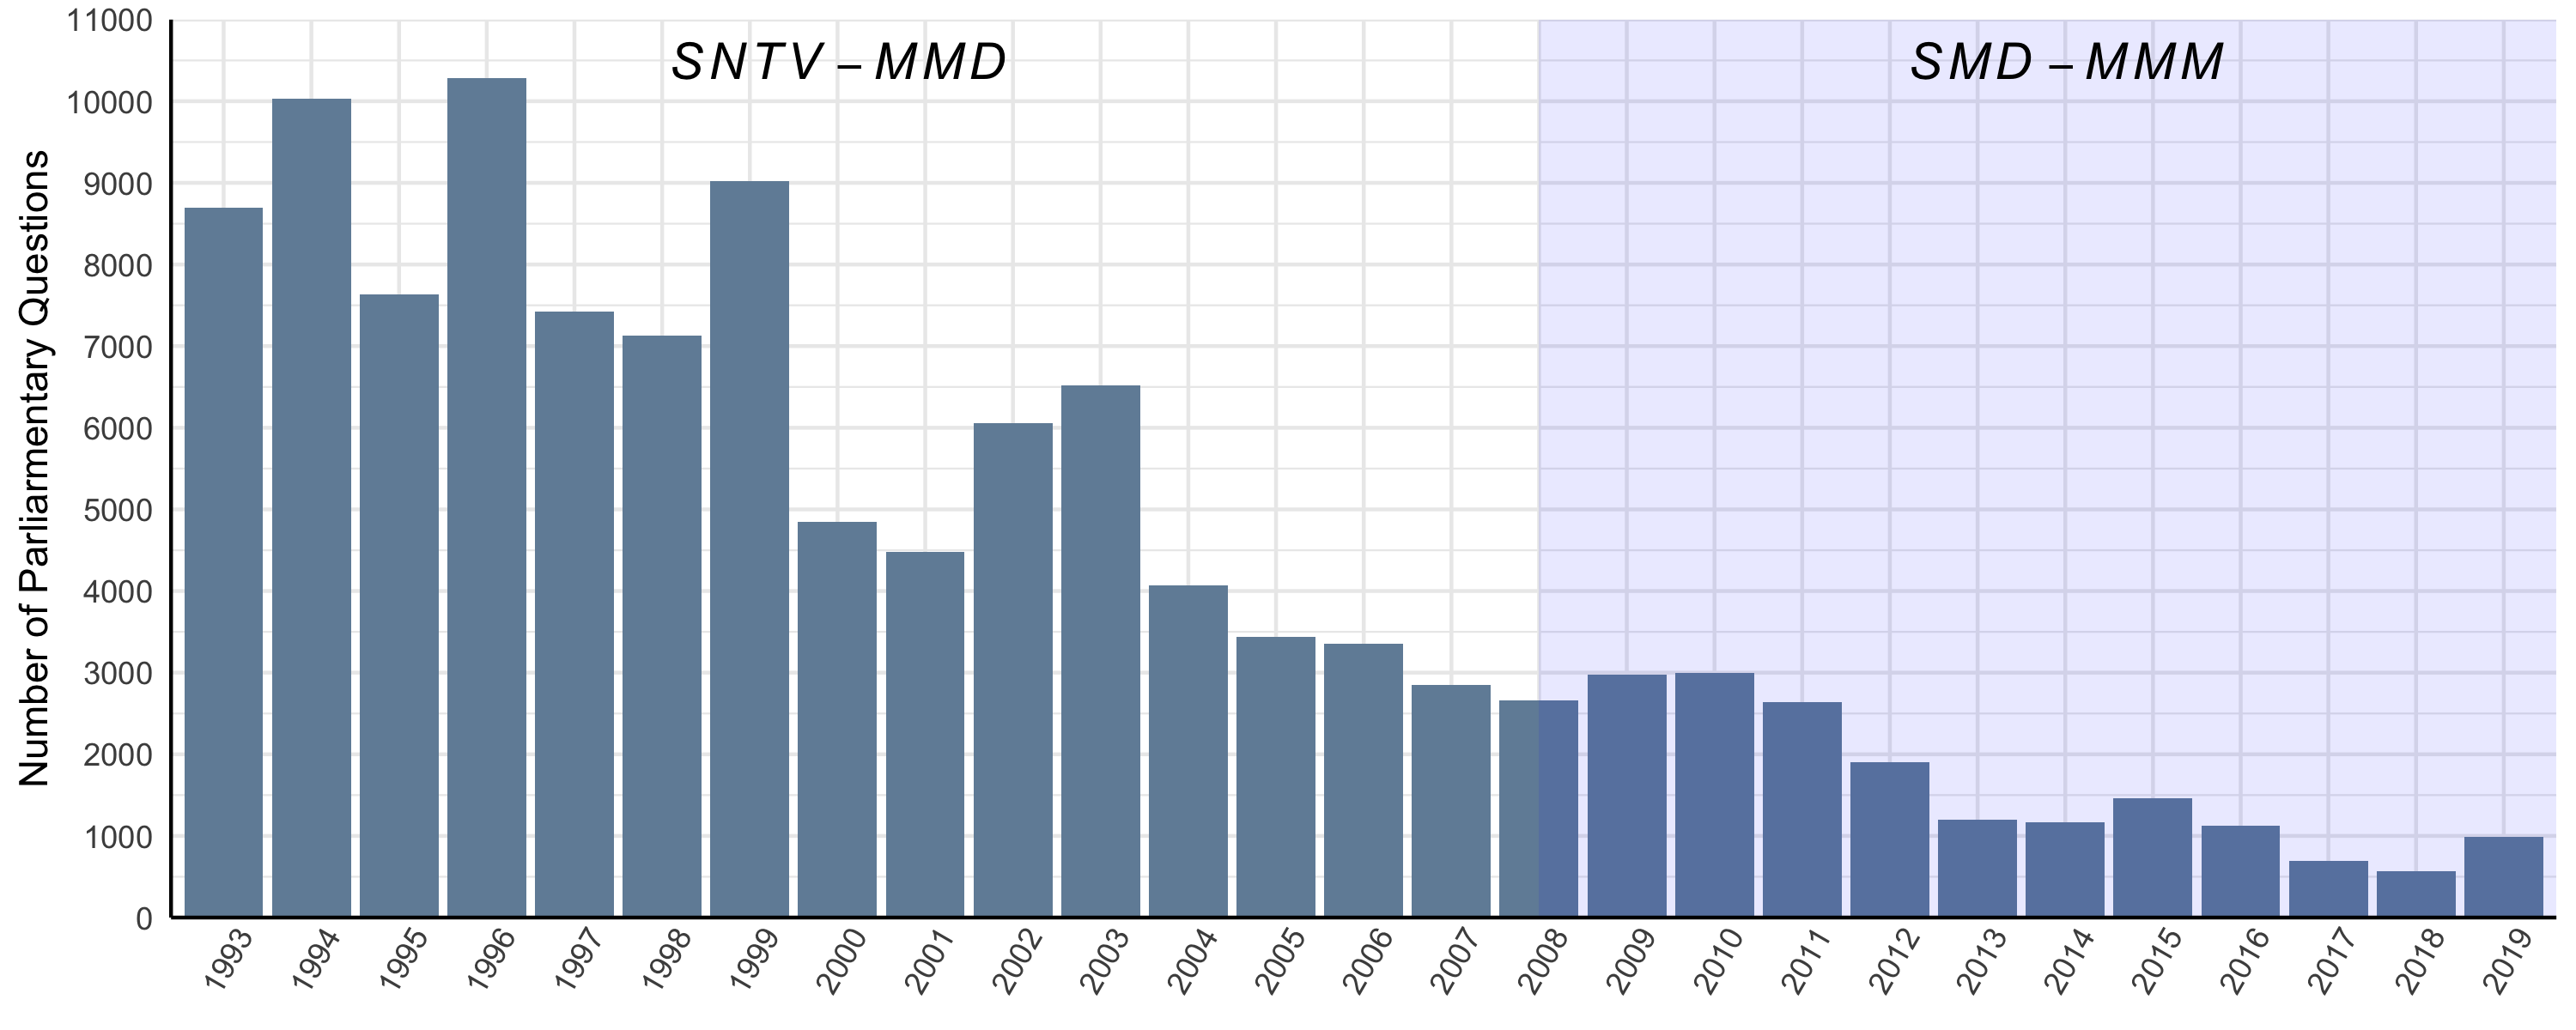
\includegraphics[width = 14.5cm, height=7.5cm]{03-Chapter-Three/image/p1.png}
    \caption{The Number of Parliamentary Questions from 1993 to 2019}
    \label{fig:pq}
    \begin{tablenotes}
    \end{tablenotes}
\end{figure}


To display the distribution of the questions across years, \autoref{fig:discriptionpq} demonstrates the total number of parliamentary questions documented from 1993 to 2019. During this period, the Taiwan legislature went through the movement of reducing legislative seats, which started in 2000, and the reform occurred in 2008. In the pre-2000 period, the number of questions asked remained roughly stable with multiple fluctuations. Nevertheless, there was a noticeable drop in the number of questions since 2000, right after the start of the movement. This trend persisted, and the total number of questions plummeted. 

The \autoref{fig:top20} shows the top 20 categories of topics that were frequently asked during the period. Topic categories related to social administration and police administration were the top two topics that appeared in the discussions in the legislature. Coming next are categories about environment and finance. 

\begin{figure}[hb!]
    \centering
    \begin{subfigure}[t]{0.48\textwidth}
    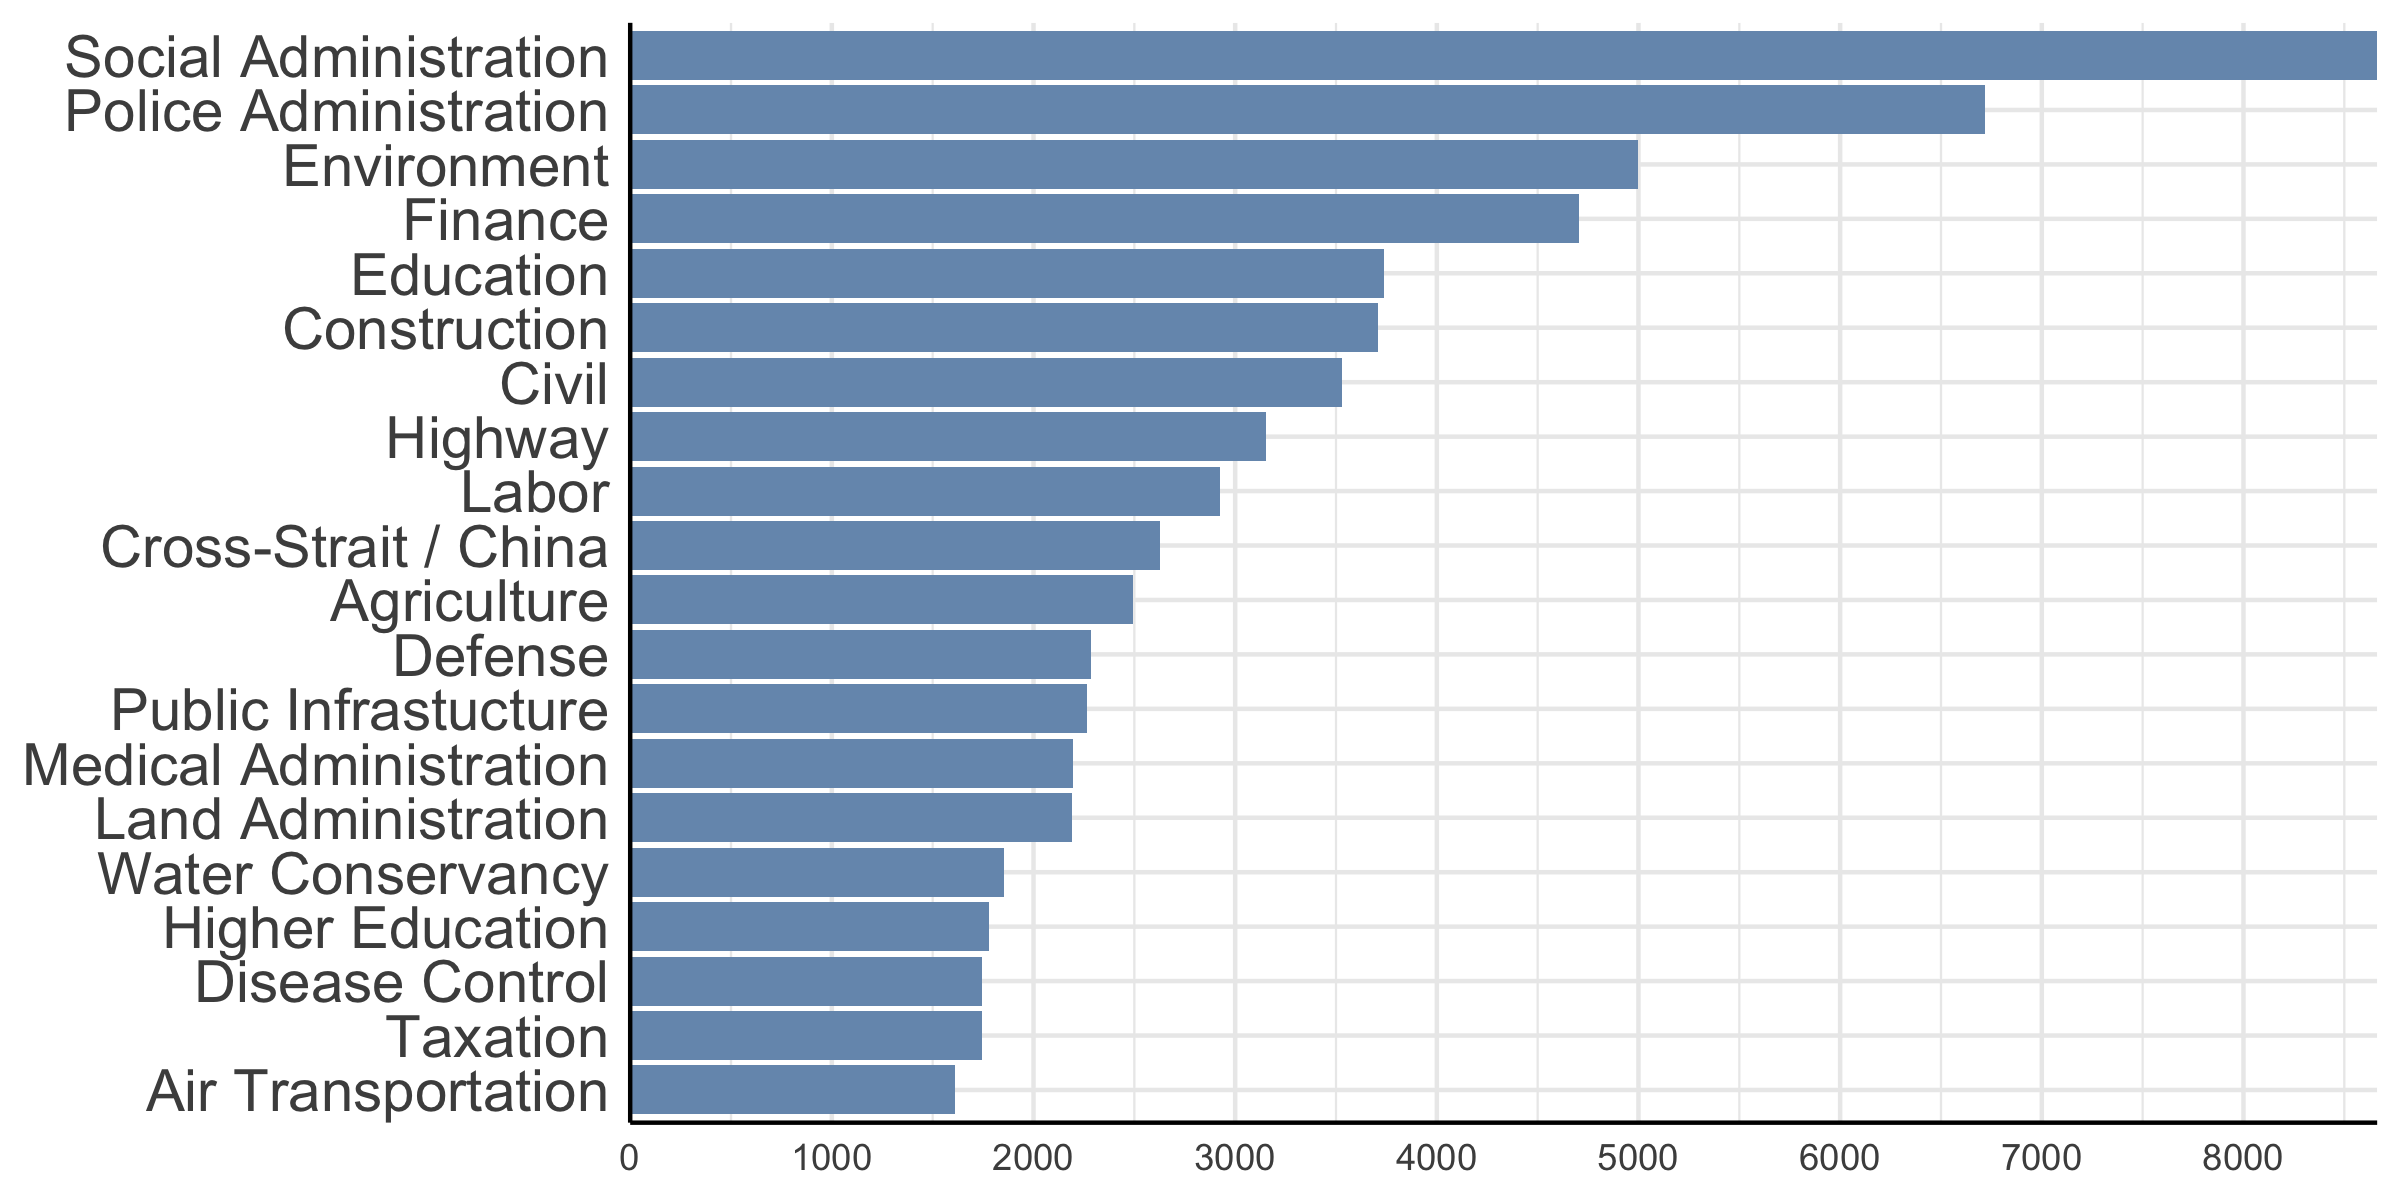
\includegraphics[width=7cm, height=5.6cm]{03-Chapter-Three/image/top20.png}
    % \caption{The Number of Parliamentary Questions from 1993 to 2019} 
    \caption{Tops 20 Most Frequent Categories} 
    \label{fig:top20}
    \end{subfigure}
    \centering
    \begin{subfigure}[t]{0.48\textwidth}
    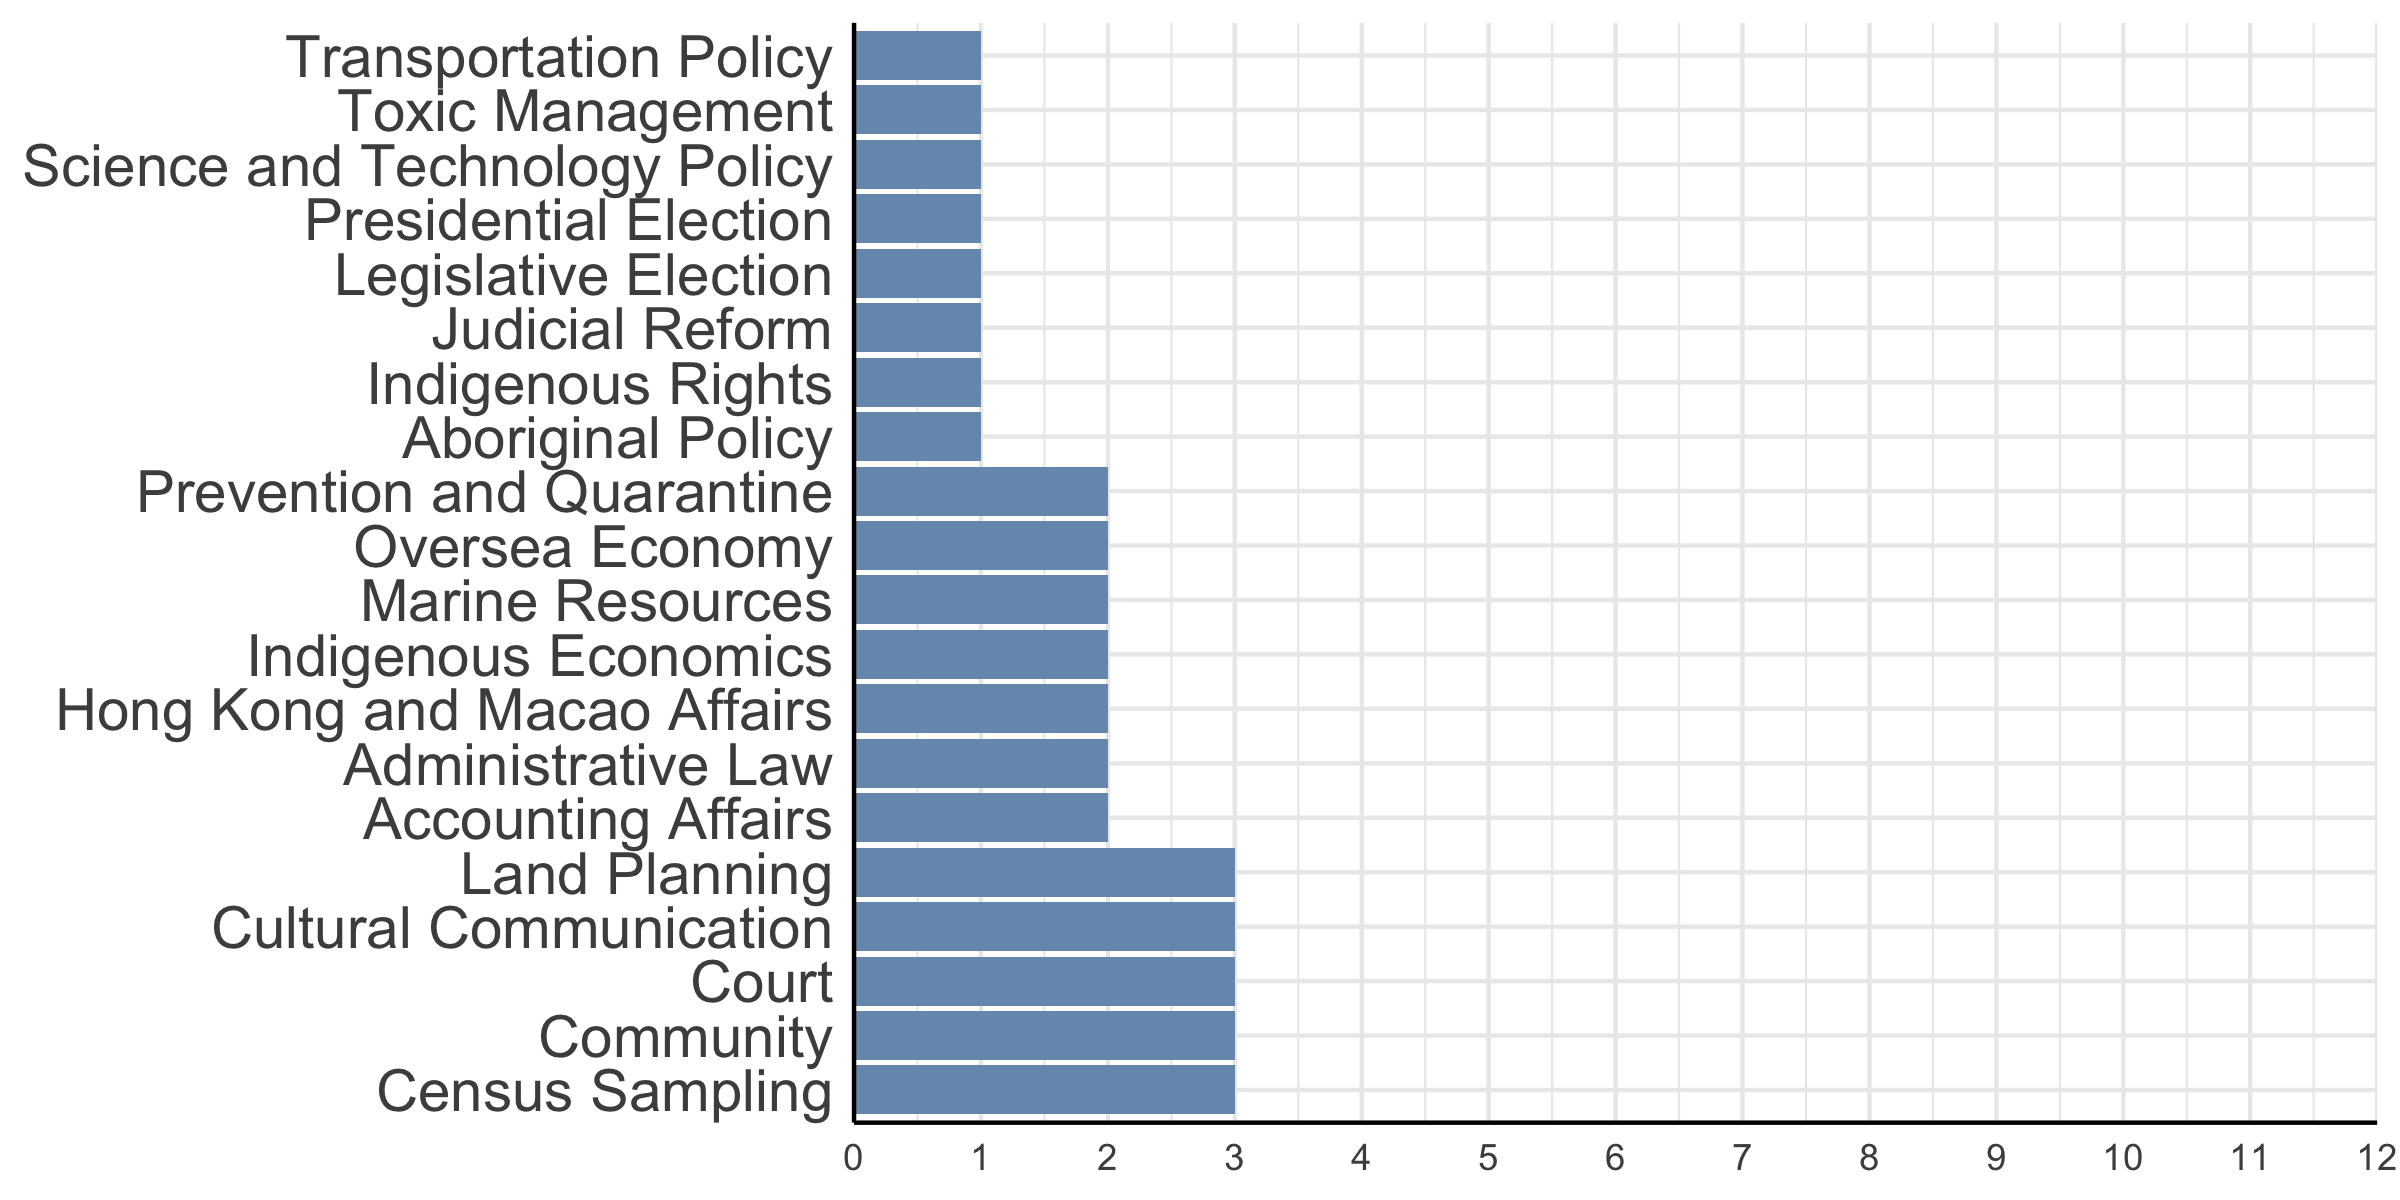
\includegraphics[width=7cm, height=5.6cm]{03-Chapter-Three/image/tail20.png}
    \caption{Top 20 Less Frequent Categories}
    \label{fig:tail20}    
    \end{subfigure}
    \caption{The Distribution of Parliamentary Questions Categories Asked by Legislators}
    \label{fig:discriptionpq}    
\end{figure}


\section*{\centering Pork Barrelling Machine Classifier}

This chapter takes advantage of using the Pork-barrel Legislation Dataset assembled by Prof. Dr Ching Jyuhn Luor \citep{Luor2008, Luor2009, Luor2012} to train the deep learning model proposed by this chapter. The collection of the dataset consists of 7243 pieces of legislation which were manually annotated as \textit{Pork (with label 1)} or \textit{Non-Pork (with label 0)} from 2004 to 2008. In addition, this data set was cross-coded by three social science researchers to assess its validity, which achieves 98\% in terms of consistency and precision among coders \citep{Luor2008,Luor2009}. 

\begin{figure}[!ht]
    \centering
    
\includegraphics[width = 14.5cm]{03-Chapter-Three/image/billeg.png}
    \caption{Pork Barrel Legislation Regarding Improving the Quality of Retired Farmers' Life}
    \label{fig:farmers}
    \begin{tablenotes}
    \end{tablenotes}
\end{figure}


The gold standard for identifying pork barrel legislation is based on the target beneficiaries of the policy (distributed vs. concentrated) and the attributes of policy cost (distributed vs. concentrated), as illustrated in \autoref{fig:type}  \citep{Wilson2001}. In particular, typical pork-barrel policies (or legislation) mainly incur distributed costs while generating parochial benefits for specific regions or designated population groups. For instance, the decision to execute an areotropolis project, which involves constructing an airport within a particular area, e.g. Taoyuan City, incurs collective costs for all Taiwanese taxpayers, while the benefit of such a particularistic project is narrowly concentrated within a parochial group of Taoyuan residents (in terms of employment opportunities, economic development, and convenience of the airport) as well as local politicians such as legislators themselves. 

Moreover, another example is the subsidy for the targeted populations. As illustrated in \autoref{fig:farmers}, the purpose of the legislation was to raise the farmers' monthly allowance from NTD 5000 to NTD 15000. In general, the majority of retired farmers are concentrated in agricultural municipalities. Thus, \citet{Luor2008, Luor2009} operationalises those concepts commonly found in Taiwan's political context and further categorises the legislation into pork and non-pork.

\begin{figure}[ht]
    \centering
    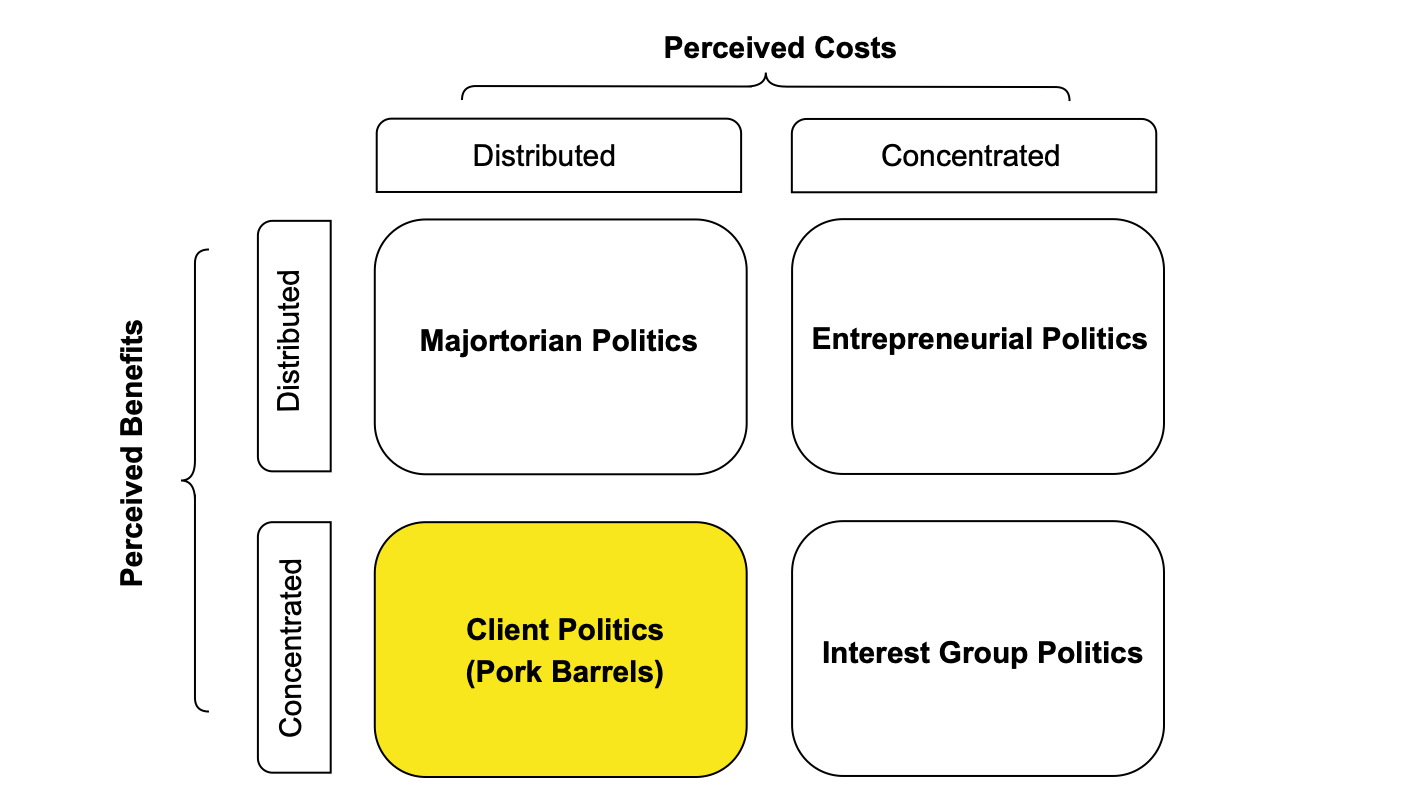
\includegraphics[width = 17cm, height=10cm]{03-Chapter-Three/image/porktype.png}
    \caption{Classifying and Explaining the Politics of Different Policy Issues, Source: \citet{Wilson2001}}
    \label{fig:type}
\end{figure}


\subsection*{Using BERT Model as Embedding Layers}

With increasingly available amounts of political data, the application of the classification task using deep learning methods has received great attention in political science \citep{Chatsiou2020}. In natural language processing, text classification assigns a set of predefined categories to open-ended documents. The approach used in this chapter is to combine one of the famous Transformer architectures, BERT developed by Google, with convolutional neural networks. 

CNN is one of powerful neural network architectures commonly applied in natural language processing \citep{Zhang2015, Zhang2020, Kim2014, Kim2016}. The architecture can be constructed by a series of convolutions and pooling layers, filtering input vectors and creating a feature map that summarizes the input texts. Then, the feature map can be stacked one over another to form a matrix by single-dimensional convolutional filters to extract high-level features. In the context of text classification task, convolution layer essentially learns the condensed features as learning image data. 

\begin{figure}[ht]
    \centering
    \begin{subfigure}[t]{0.45\textwidth}
    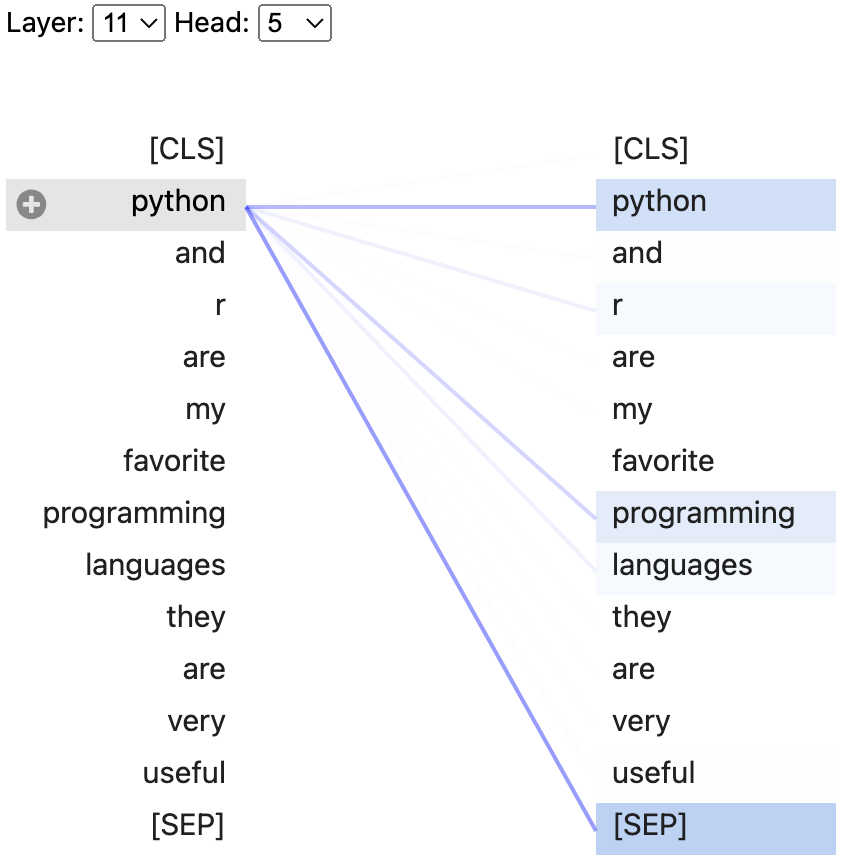
\includegraphics[width=7cm, height=6cm]{03-Chapter-Three/image/vis2.png}
    \caption{Sentence 1: Python refers programming language}
    \label{fig:python1}
    \end{subfigure}
    \centering
    \begin{subfigure}[t]{0.45\textwidth}
    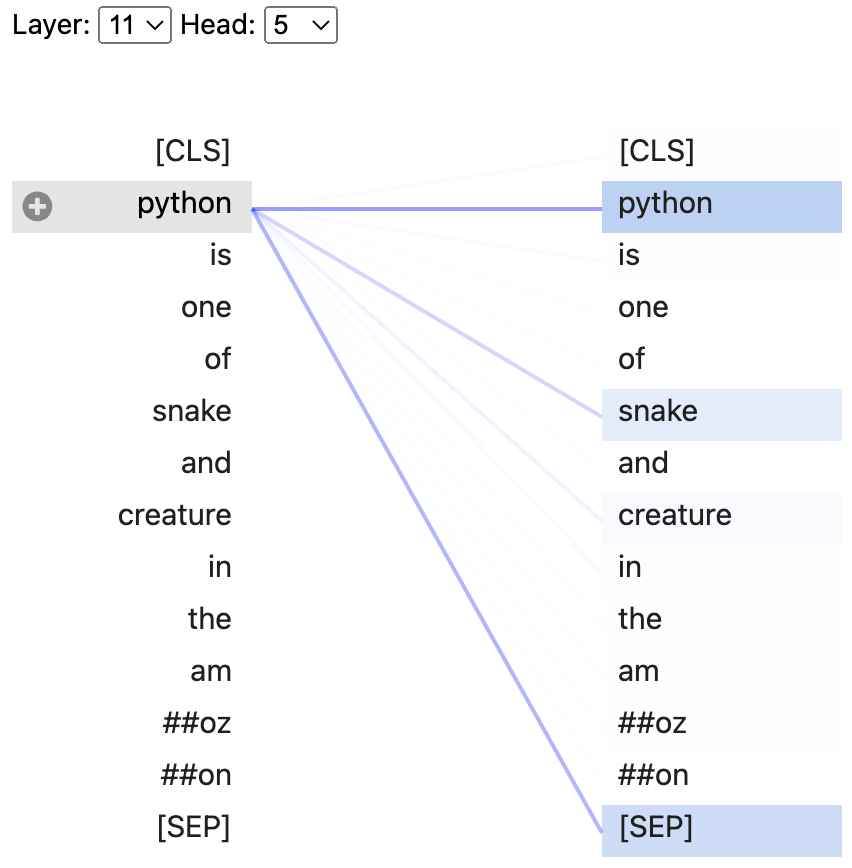
\includegraphics[width=7cm, height=6cm]{03-Chapter-Three/image/vis3.png}
    \caption{Sentence 2: Python refers snake}
    \label{fig:python2}    
    \end{subfigure}
    \caption{An Example of Self-attention Mechanism in BERT  Transformer Using 
    Pretrained model on English language (\href{https://huggingface.co/bert-base-uncased}{bert-base-uncased})
    % \footnote{Visualization using BertViz library\citep[see,][]{vig-2019-multiscale}}
    }
    \label{fig:visbert}    
\end{figure}

In practice, the convolutional layers (or recurrent neural net) are recently introduced as encoders or decoders to deal with semantics problems in modern application of natural language processing. Generally, we can transform input texts with embedding models such as Word2Vec, GloVe or one-hot vector. However, the major challenge of these approaches lies in the fundamental assumption that each input word has fixed representation in different contexts, introducing a potentially severe problem of misrepresentations by referring to inaccurate meaning across sentences. For example, the embedding word ``python'' as shown in \autoref{fig:visbert} can have different meanings depending on the language context in which it appears. Regardless of polysemous mean in different sentences, the word ``python'' only renders the same vector. This is because traditional embedding models are context-free, which gives static embedding vectors for the word ``python''. 

Contrary to earlier approaches, BERT is one of the most powerful Transformer architectures that can detect input tokens in bidirectional semantic context with its prominent feature called self-attention \citep{Devlin2019, Vaswani2017}.\footnote{BERT is the first contextual-based model based on the transformer architecture released by Google.  Transformers models also include ALBERT, RoBERTa, DistilBERT, GPT2 and others.} Theoretically, BERT consists of 12 encoder layers, stacked over one another as shown in \autoref{fig:bert}, respectively. For example, giving the single word ``python'' in two different contexts in \autoref{fig:visbert},  ``python'' in \autoref{fig:python1} refers to one of the programming languages because contextual embedding is highly associated with ``programming'', ``languages'', and ``r (statistical computing language)''. On the other hand, ``python'' in \autoref{fig:python2} refers to an animal in the sentence context as its representation embedding is correlated with snake and creature.

As discussed above, self-attention is a mechanism that allows neural networks to assign a different amount of attention weight to each element to compute representation embedding in a sequence. This is powerful for performing NLP tasks when dealing with unseen words or tokens not included in the static embedding model like Word2Vec.   

\begin{figure}[htbp]
    \centering
    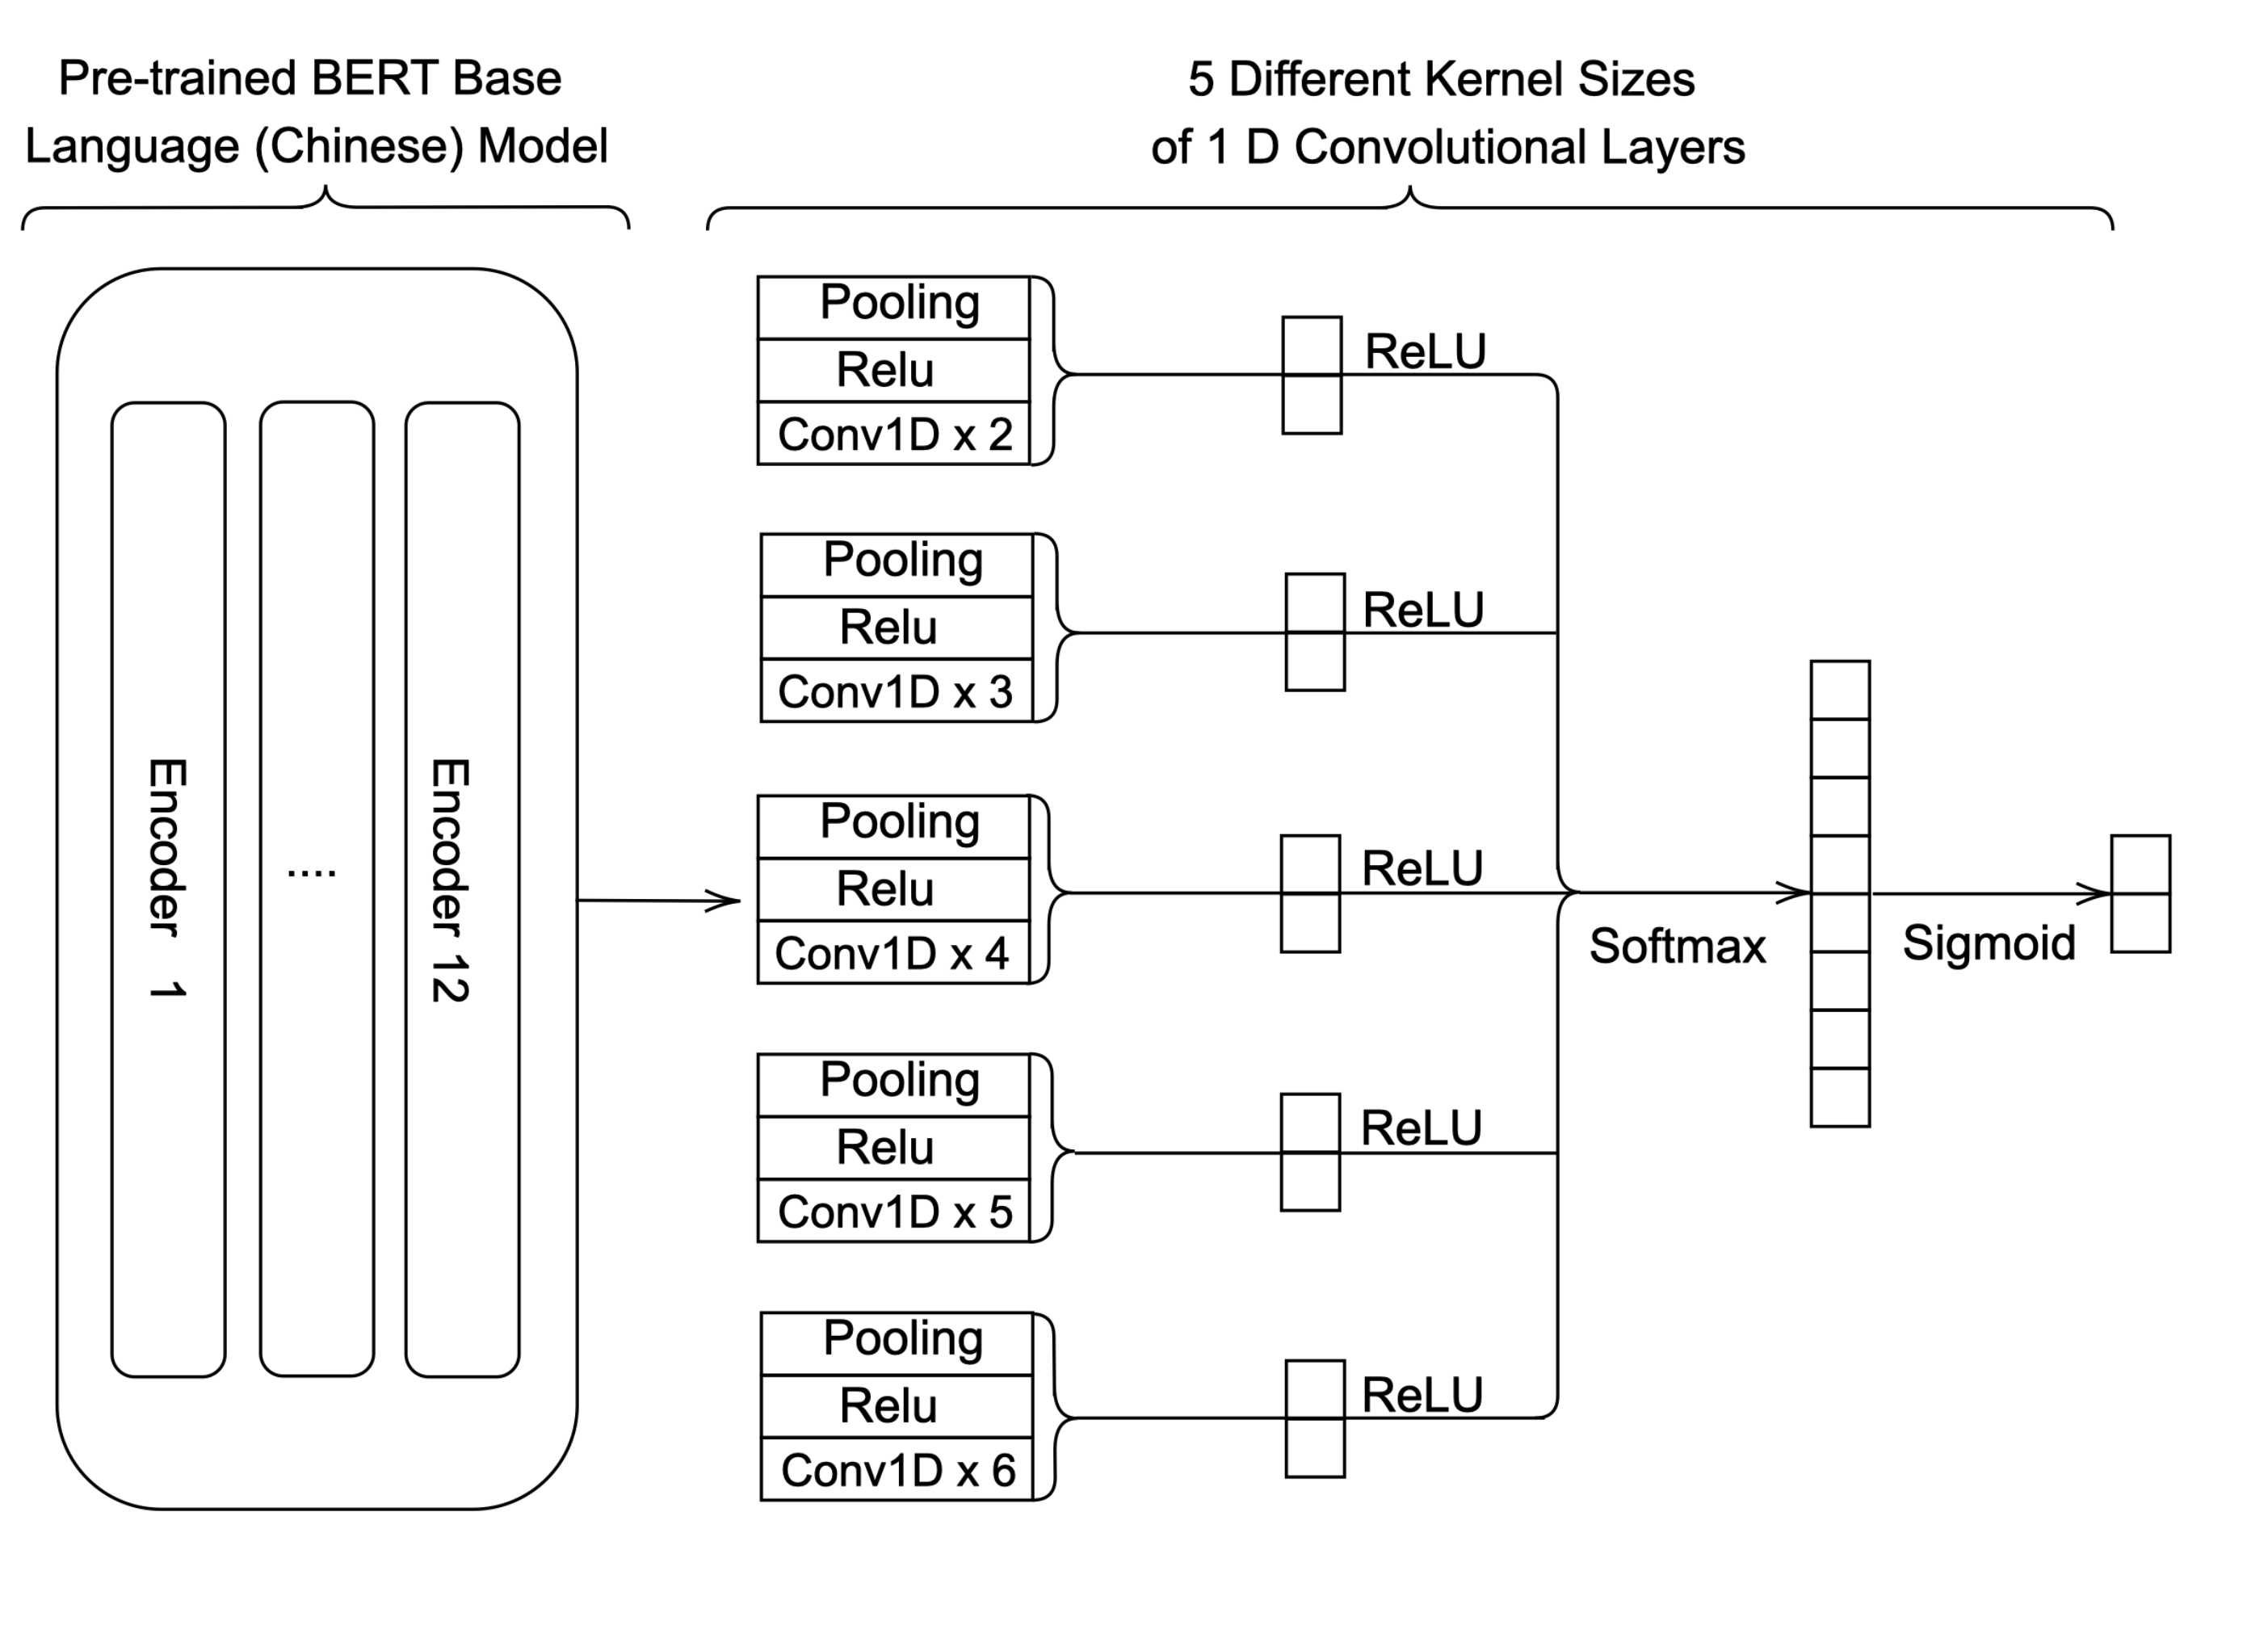
\includegraphics[width = 14.5cm, height=9.1cm]{03-Chapter-Three/image/framework.png}
    \caption{The Designed Architecture for Pork Barrel Classification Task}
    \label{fig:bert}
    \begin{tablenotes}
    \end{tablenotes}
\end{figure}

\subsection*{Combining Convolutional Neuralnet with BERT Embedding Layer}
Combining CNN with BERT for classification tasks is getting popular in natural language processing in recent years \citep{Safaya2020, Lu2019, Lopez2017}. For example, \citet{Safaya2020} use convolutional layers followed by BERT embedding to create a machine learning model that deals with offensive speech identification, while \citet{Lu2019} deploying the similar approach to patent document classification. Those performance of combination approach is drastically improved from the character-based CNN and the generic BERT model, respectively. The innovative design for machine learning architecture in the literature that motivates the model used is the following. I create the architecture for detecting pork-barrel features in parliamentary questions, as shown in \autoref{fig:bert}. All the encoders use 12 attention heads and 12 layers. Theoretically, each token can be represented as 768 hidden units \citep[][]{Wolf2020}.\footnote{The traditional Chinese BERT model used in the chapter is \textit{bert-base-Chinese} which is maintained by CKIP (Chinese Knowledge and Information Processing) at the Institute of Information Science and the Institute of Linguistics, Taiwan Academia Sinica.} 

First, I transform each word in the sentence with its word vector using the Chinese BERT pre-trained model.\footnote{This model can be downloaded from \href{ https://ckip-transformers.readthedocs.io/en/stable/}{ https://ckip-transformers.readthedocs.io/en/stable/} and \textit{HuggingFace} at \href{https://huggingface.co/bert-base-chinese}{https://huggingface.co/bert-base-chinese}.}  In the BERT layer, I can feed input sentences (pork legislation text) in the encoder layer, where the encoder learns the representation. Afterwards, the decoder generates new output based on the patterns understood by the following encoder. In order to fit embedding vector into CNN layers, I create five kernels of different lengths, aiming to capture different patterns of the n-gram in the original sentence. After the output is passed through ReLU activation, Global Max Pooling is introduced to flatten high-dimensions feature maps into two-dimensional vectors. At the last set of layers, I use the Sigmoid function commonly adapted for binary class with dense layers to get the final outcome, which is the probability of being classified as pork-barrel project.\footnote{Regarding model performance metrics, see \autoref{tab:performance} in Supplementary Appendix \ref{tag:performance} }



\begin{table}[h]
\caption{Sampled Parliamentary Questions Being Most Likely to Mention Particularistic Goods}
\centering
\scalebox{0.68}{
    \begin{tabular}[t]{l*{4}{c}} 
    \toprule 
    Legislators               & 
    Probability of Being Pork &   
    Topics                    &
    Keywords                  &
    Questions \\ [0.8ex]
    \hline
    林正峰 & 0.995515823364258 & Health Insurance     & Health Insurance Deductions & 特别扣除额教育支出...\\
    彭添富 & 0.992780447006226 & Aboriginal Affair    & Housing Subsidies & 
    而非采用扣除免税额...\\
    李復興 & 0.992780089378357 & Old-age Benefits     & Elderly Allowance & 
    原住民家庭租屋補助...\\
    盧秀燕 & 0.992639720439911 & Veterans Welfare     & Grants for Retired Veterans & 
    補助金發放金額過低...\\   
    李顯榮 & 0.990033149719238 & Farmer Welfare       & Subsidies; Allowance  & 
    政府前後援賽金額高...\\   
    丁守中 & 0.988385319709778 & The Handicapped      & Living Allowance  & 
    身心障礙者生活津貼...\\   
    馮定國 & 0.985531985759735 & Elderly Welfare      & Unemployment Fund &
    高齡失業問題嚴重日...\\   
    彭添富 & 0.983698368072510 & Agriculture          & Crops Subsidies &
    農作物損失補償問題...\\   
    曾華德 & 0.979519009590149 & Military Affair      & Increased Pay  &
    救国军补发薪饷问题...\\   
    林鴻池 & 0.978044390678406 & Education            & University Subsidy &
    針對諸多已獲得五年...\\   
    
        \bottomrule
        \end{tabular} }
    \label{table:pork}
\end{table}

To validate the classification quality, I sampled 20 pork and non-pork questions respectively in \autoref{table:pork} and \autoref{table:nonpork}, automatically classified by the architecture in \autoref{fig:bert}. I merge these questions with corresponding keywords and categories (translated to English) scraped from the website of Taiwan Legislative Yuan. As shown in \autoref{table:pork}, most pork-barrel questions are associated with central government spending for targeted groups and localised infrastructure projects mainly allocated to specific regions. Some legislators raise the question of asking the central government to increase rent subsidies for the aboriginal population, while others target policies related to relief and support programmes such as crop subsidy and elderly allowances for specific groups in some municipalities located in western Taiwan. In addition to \autoref{table:nonpork} demonstrate many examples of non-particularistic questions. For instance, the questions of keywords and topics are very closely related to regulatory and national policies such as railway management, drug control and criminal investigation. 

% Table \ref{table:pork} displays the most possible of being pork-barrel quantities, whereas Table \ref{table:nonpork} exemplifies the number of sample questions that are more likely to label non-pork-barrel features. 


\begin{table}[ht]
\caption{Sampled Parliamentary Questions Being Less Likely to Mention Particularistic Goods }
\centering
\scalebox{0.68}{
    \begin{tabular}[t]{l*{4}{c}} 
    \toprule
    Legislators               &
    Probability of Being Pork &   
    Topics                    &
    Keywords                  &
    Questions               \\ [0.8ex]
\hline
    李復甸 & 0.000021549063604 & Litigation Procedure & Criminal Investigation &
    鑑於刑事偵察實務上...\\
    林建榮 & 0.000020212990421 & Financial Management & Revolving Interest Rate &
    明定信用卡、現金卡...\\
    林正峰 & 0.000019731034627 & Energy Policy        & Energy Saving  & 
    要求各級機關和學校...\\
    林正峰 & 0.000019187420548 & Tobacco Restriction  & Departmental Hospital &
    毒品氾濫,吸毒人數...\\   
    王幸男 & 0.000017634354663 & Public Safety        & Road Quality & 
    針對道路人孔蓋或管...\\   
    管碧玲 & 0.000013002485503 & Railway Management   & Taiwan Railway &
    台灣鐵路管理局發生...\\   
    郭榮宗 & 0.000004869816621 & District Court       & Drug Abuse & 
    知名提神飲料遭下毒...\\   
    陳朝龍 & 0.000011277100384 & Infectious Disease   & Avian Influenza  &
    英國政府宣稱台灣出...\\   
    林進興 & 0.000007685628589 & Banking Management   & Credit Card  &
    行政院金融監督管理...\\   
    潘孟安 & 0.000002590457370 & Election             & Legislative Elections &
    單一選區兩票制即將...\\   
        \bottomrule
        \end{tabular} }
\label{table:nonpork}
\end{table}


\section*{\centering Heterogeneous Effects on Different Sizes of Parties}

I next examine the distribution of pork-barrel questions aggregated by party level from 1993 to 2019. \autoref{fig:sumpork} displays the distribution of the total number of pork-barrel questions that were requested by legislators from two major parties and the small parties, respectively, as is classified by the deep learning architecture. The left subplot for the two majority parties, KMT (Chinese Nationalist Party) and DPP (Democratic Progress Party), roughly shares a similar pattern as in \autoref{fig:pq}, with a decreasing trend of the numbers overtime after the initiation of the movement that started around 2000. The right subplot \autoref{fig:sumporksmall} shows the multiple plummets and rises 
in the total number of questions raised by small parties such as NP (New Party 新黨), PFP (People First Party 親民黨), NPSU (Non-Partisan Solidarity Union, 無黨團結聯盟), TIP(Taiwan Independence Party 台灣獨立黨), TSU(Taiwan Solidarity Union 台灣團結聯盟) and newly established MKT (the Republican Party as known as Minkuotang).

\begin{figure}[ht]
    \centering
    \begin{subfigure}[t]{0.48\textwidth}
    \centering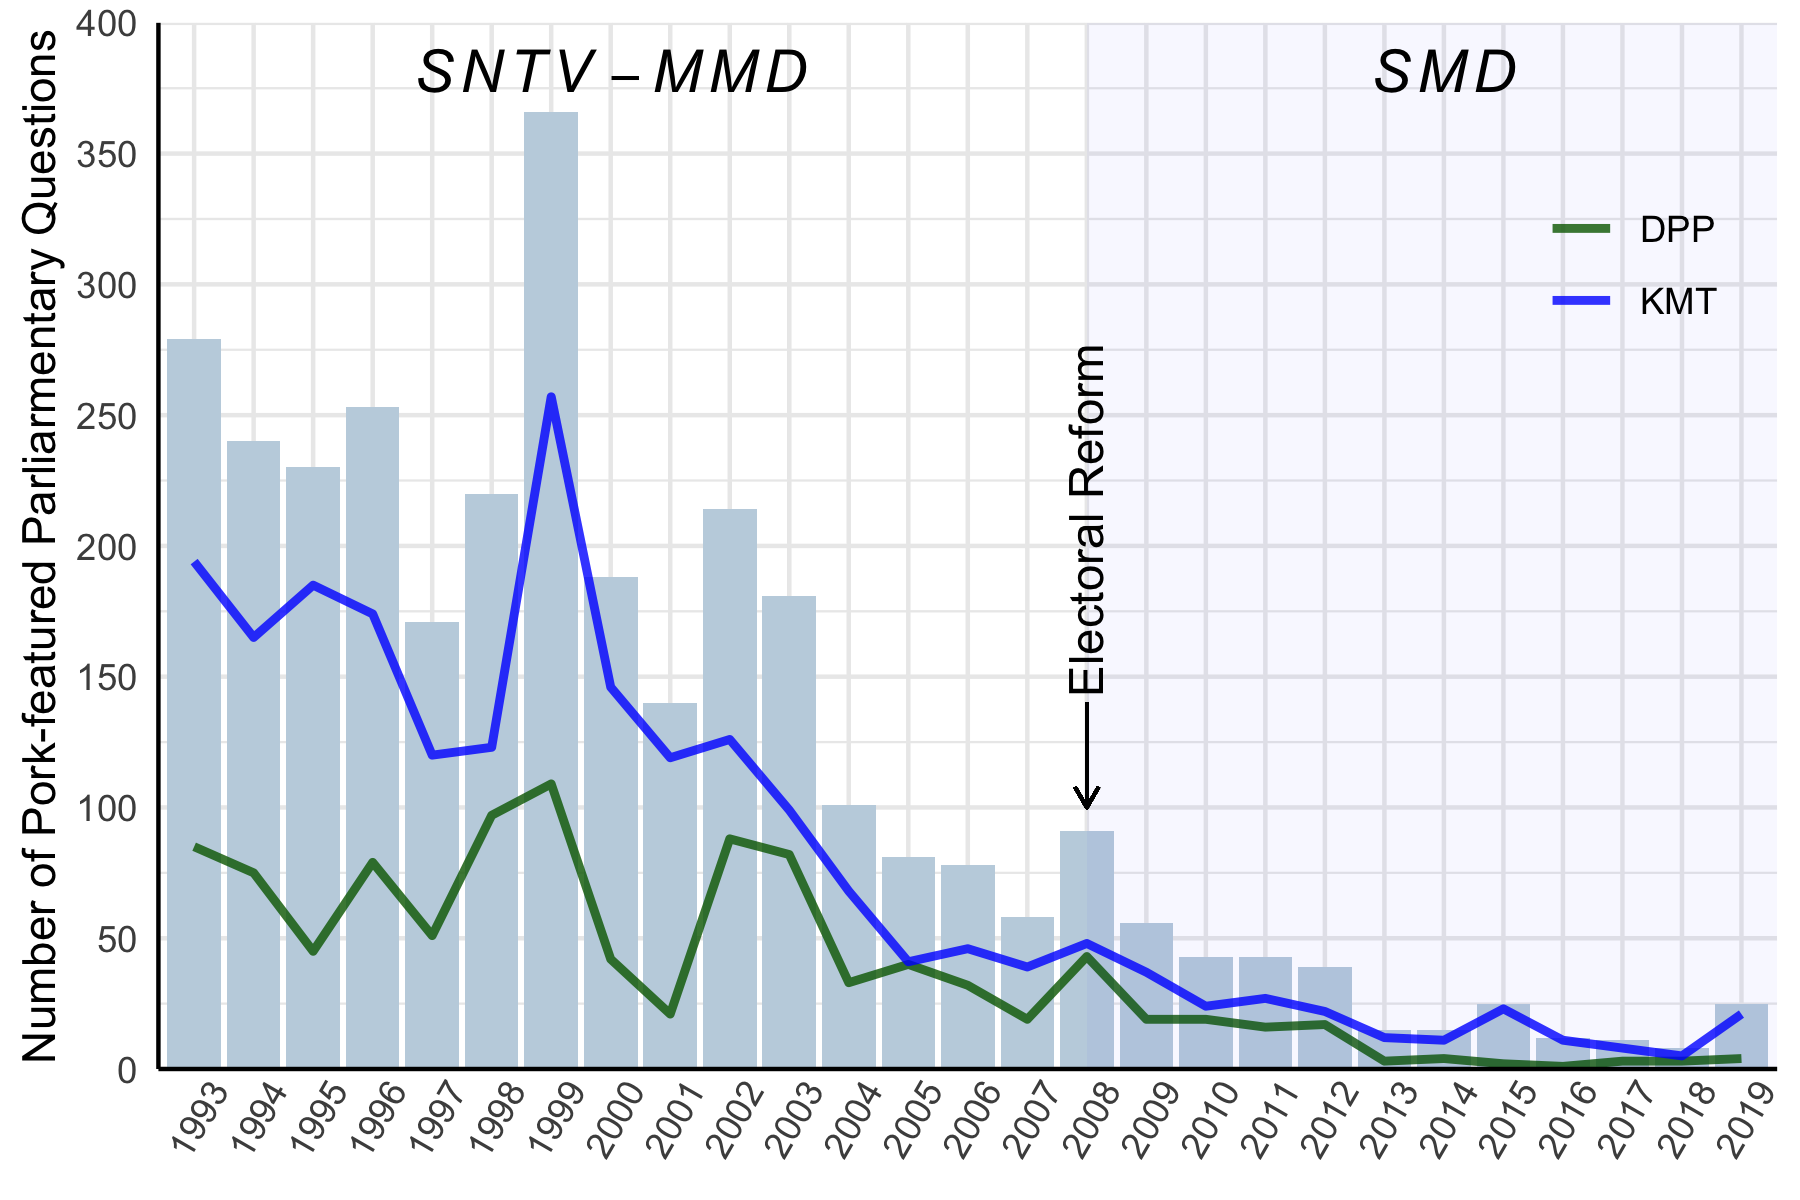
\includegraphics[width=7.2cm, height=6cm]{03-Chapter-Three/image/bigpq.png}
    \caption{Large Parties}
    \label{fig:sumporkbig}
    \end{subfigure}
    \begin{subfigure}[t]{0.48\textwidth}
    \centering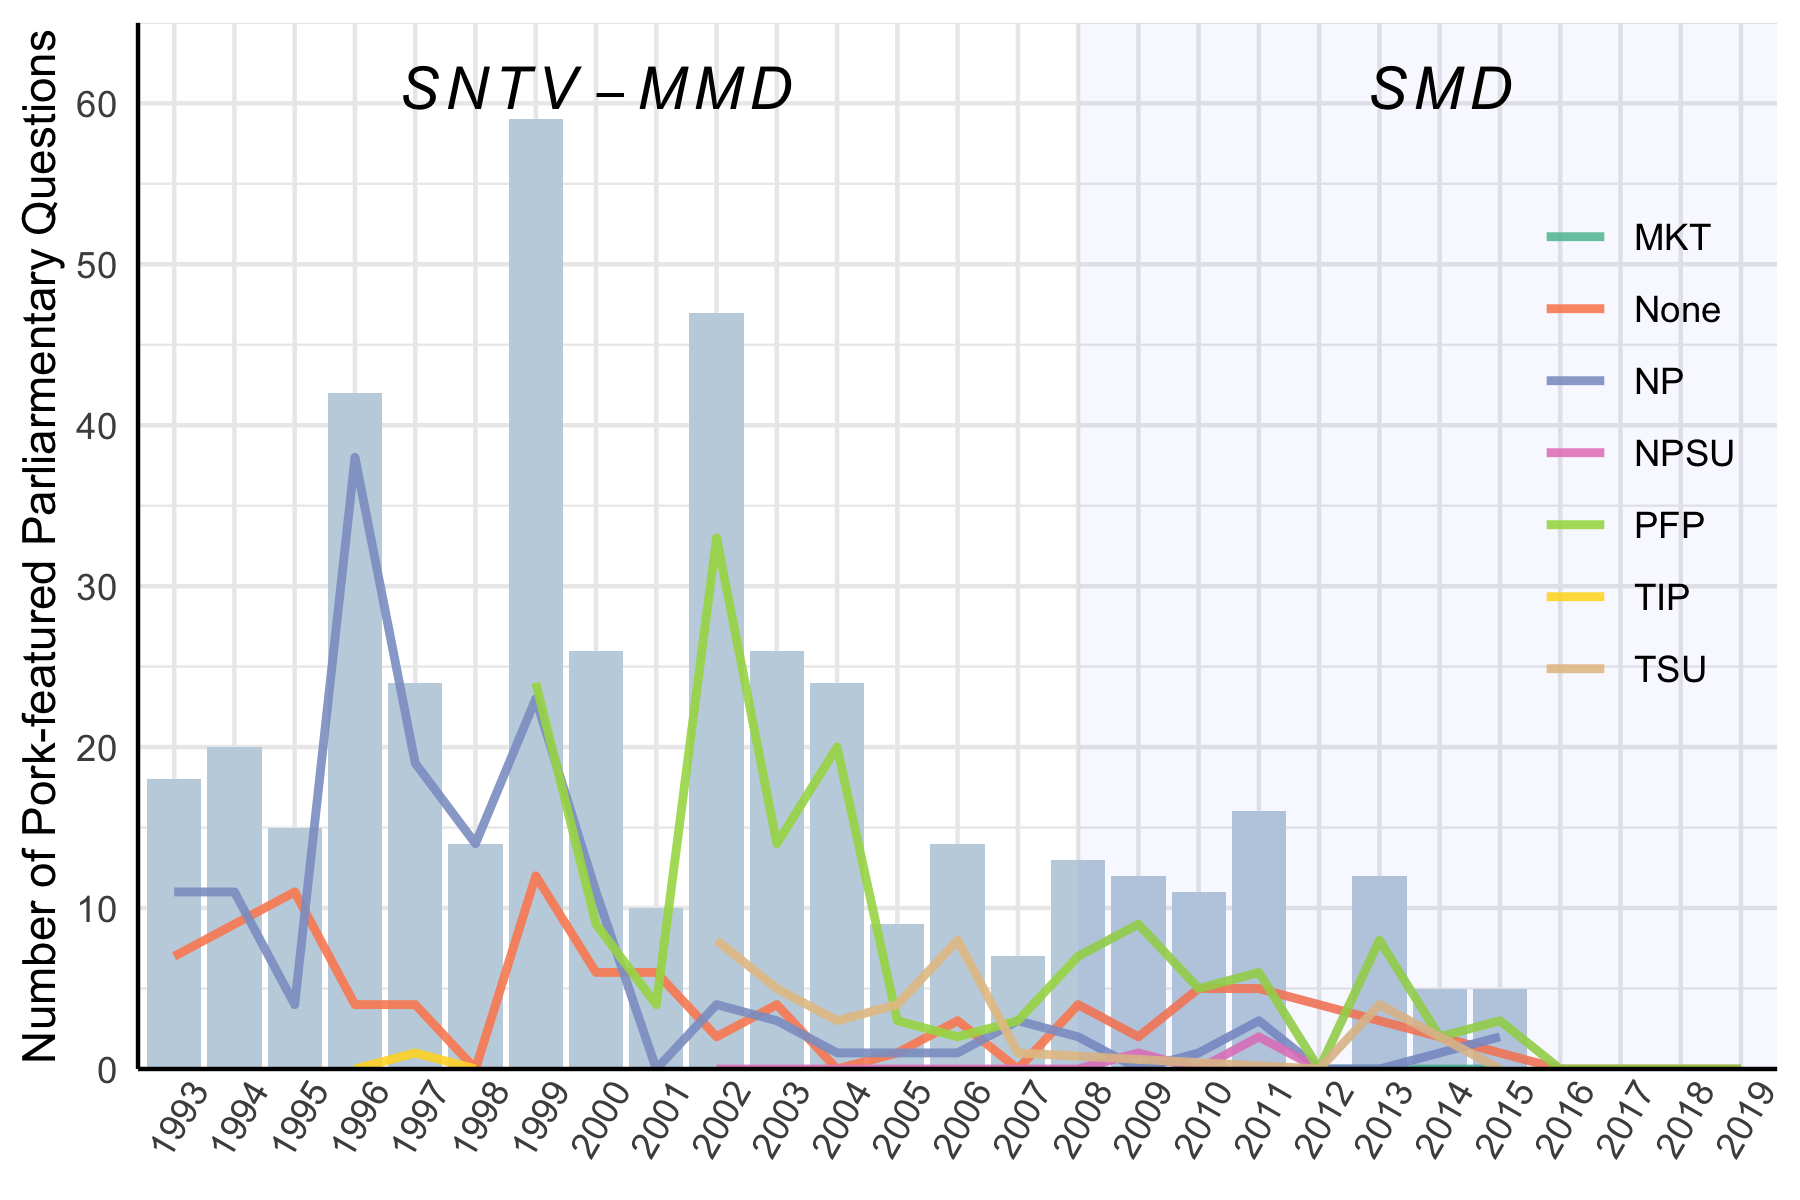
\includegraphics[width=7.2cm, height=6cm]{03-Chapter-Three/image/smallpq.png}
    \caption{Small Parties}
    \label{fig:sumporksmall}    
    \end{subfigure}
    \caption{The Number of Pork Barrel Question by Years}
    \label{fig:sumpork}    
\end{figure}


For \autoref{fig:sumpork}, the changes in the total numbers across times show that parliamentary questions are dwindling steadily, implying that legislators may alternatively use other tools to influence policy for their constituents, such as social media. For example, empirical evidence shows that district members mention more geographical terms on their Facebook and Twitter, whereas party-list members have less tendency to secure pork-barrel projects. In particular, the total number of seats was reduced from 225  to 113 after the reform. In the new system, only  73 seats are elected by district, explaining a fall-off in the number of pork-question since the reform occurred in 2008.

To exclude the effect of volatility in the number of seats across years, I illustrate the average number of pork-barrel questions per seat in the legislature. \autoref{fig:meanpork} plots the average number of questions per seat devoted to pork-barrel project for majority parties (\autoref{fig:meanporkbig}) and small parties (\autoref{fig:meanporksmall}), respectively. The actual impacts of the reform seem heterogeneous on small parties and large parties (KMT and DPP). In \autoref{fig:meanporkbig}, for large parties, the average number persistent declined from around 2001 to 2015, although there was a significant bounce back since 2017. Generally speaking, there are variations in the number of pork questions asked by small-party legislators, compared with legislators from KMT and DPP. From 2003 to 2012, the number of pork questions asked by each legislator from small parties was twice the size of large-party legislators. However, the reform differed from what I expected regarding small-party legislators: their average number increased from 2001 to 2009, yet this trend stopped in 2007. Afterwards, the trend became downward sloping, and the average number kept declining.

\begin{figure}[!ht]
    \centering
    \begin{subfigure}[t]{0.48\textwidth}
    \centering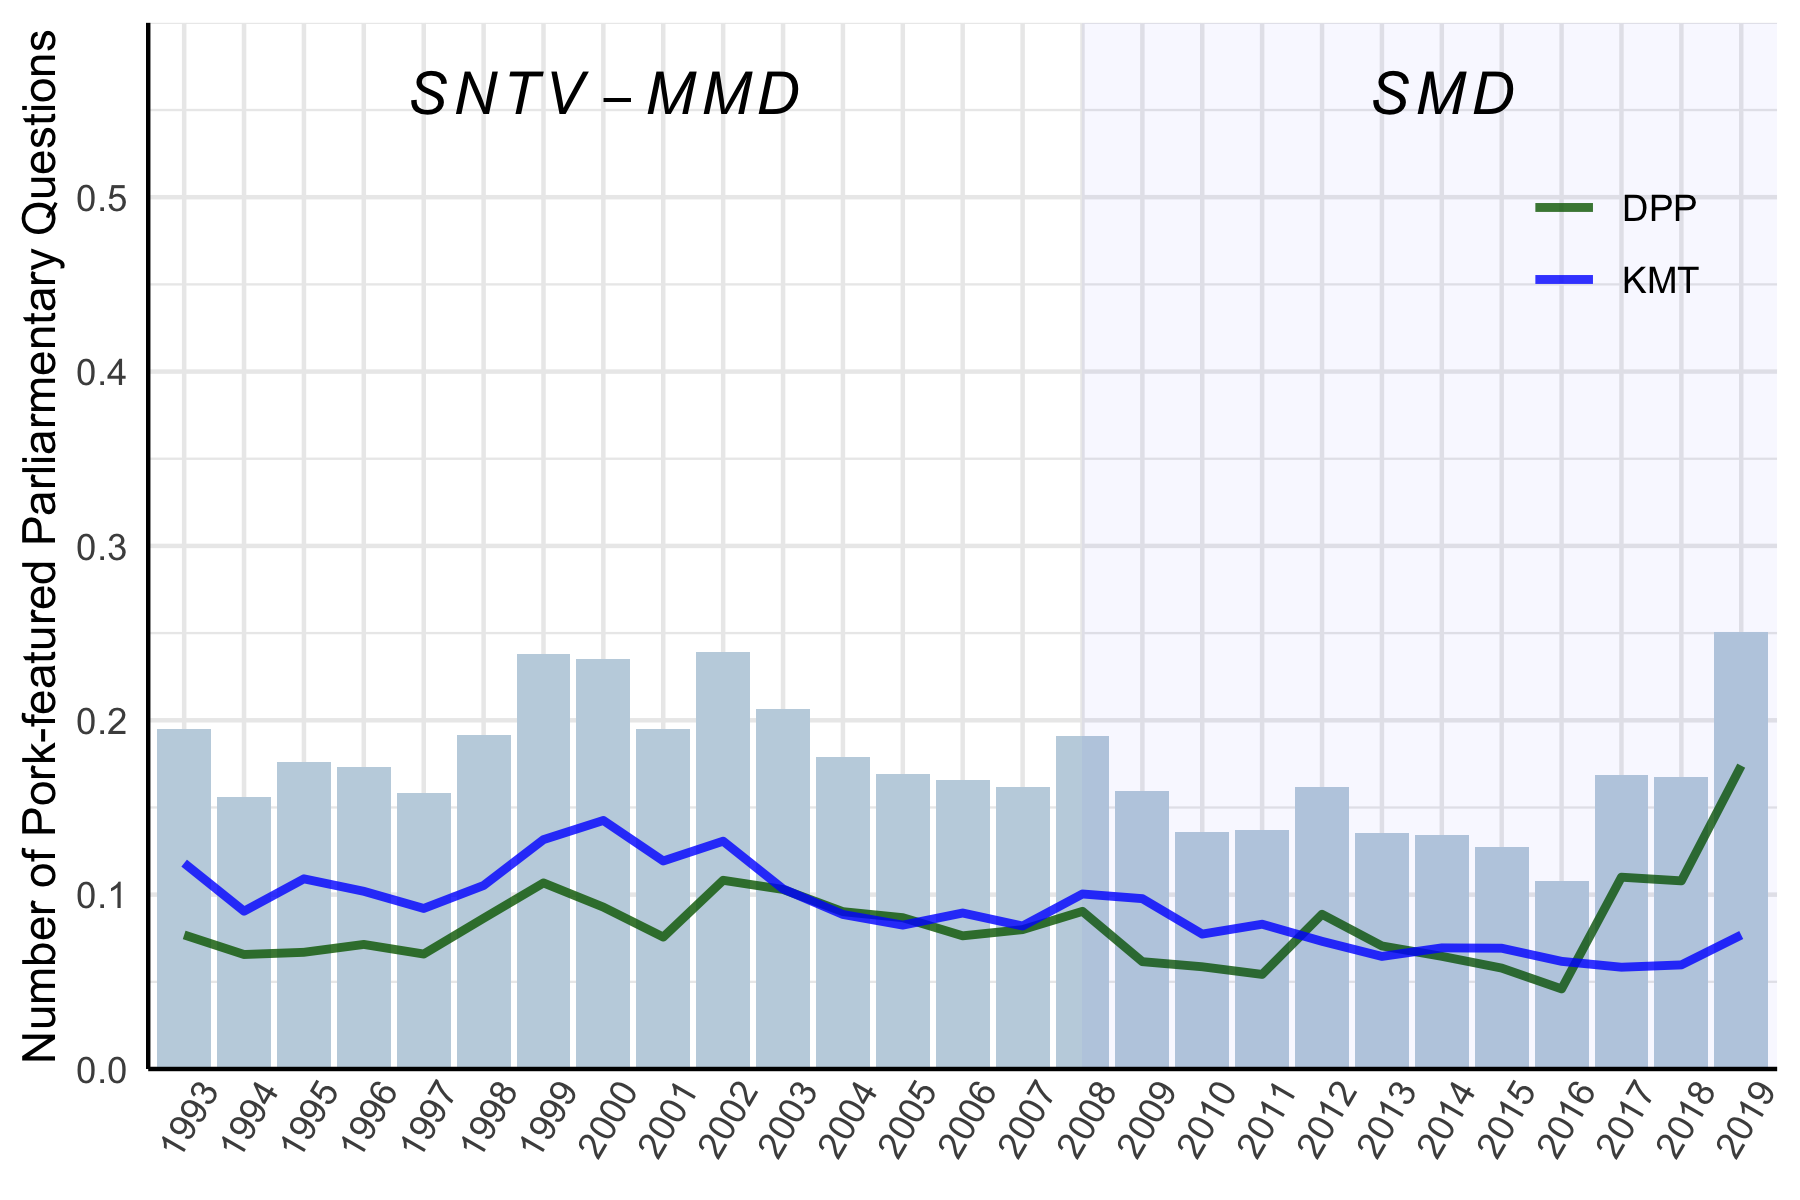
\includegraphics[width=7.2cm, height=6cm]{03-Chapter-Three/image/bigpqmean.png}
    \caption{Large Parties}
    \label{fig:meanporkbig}
    \end{subfigure}
    \centering
    \begin{subfigure}[t]{0.48\textwidth}
    \centering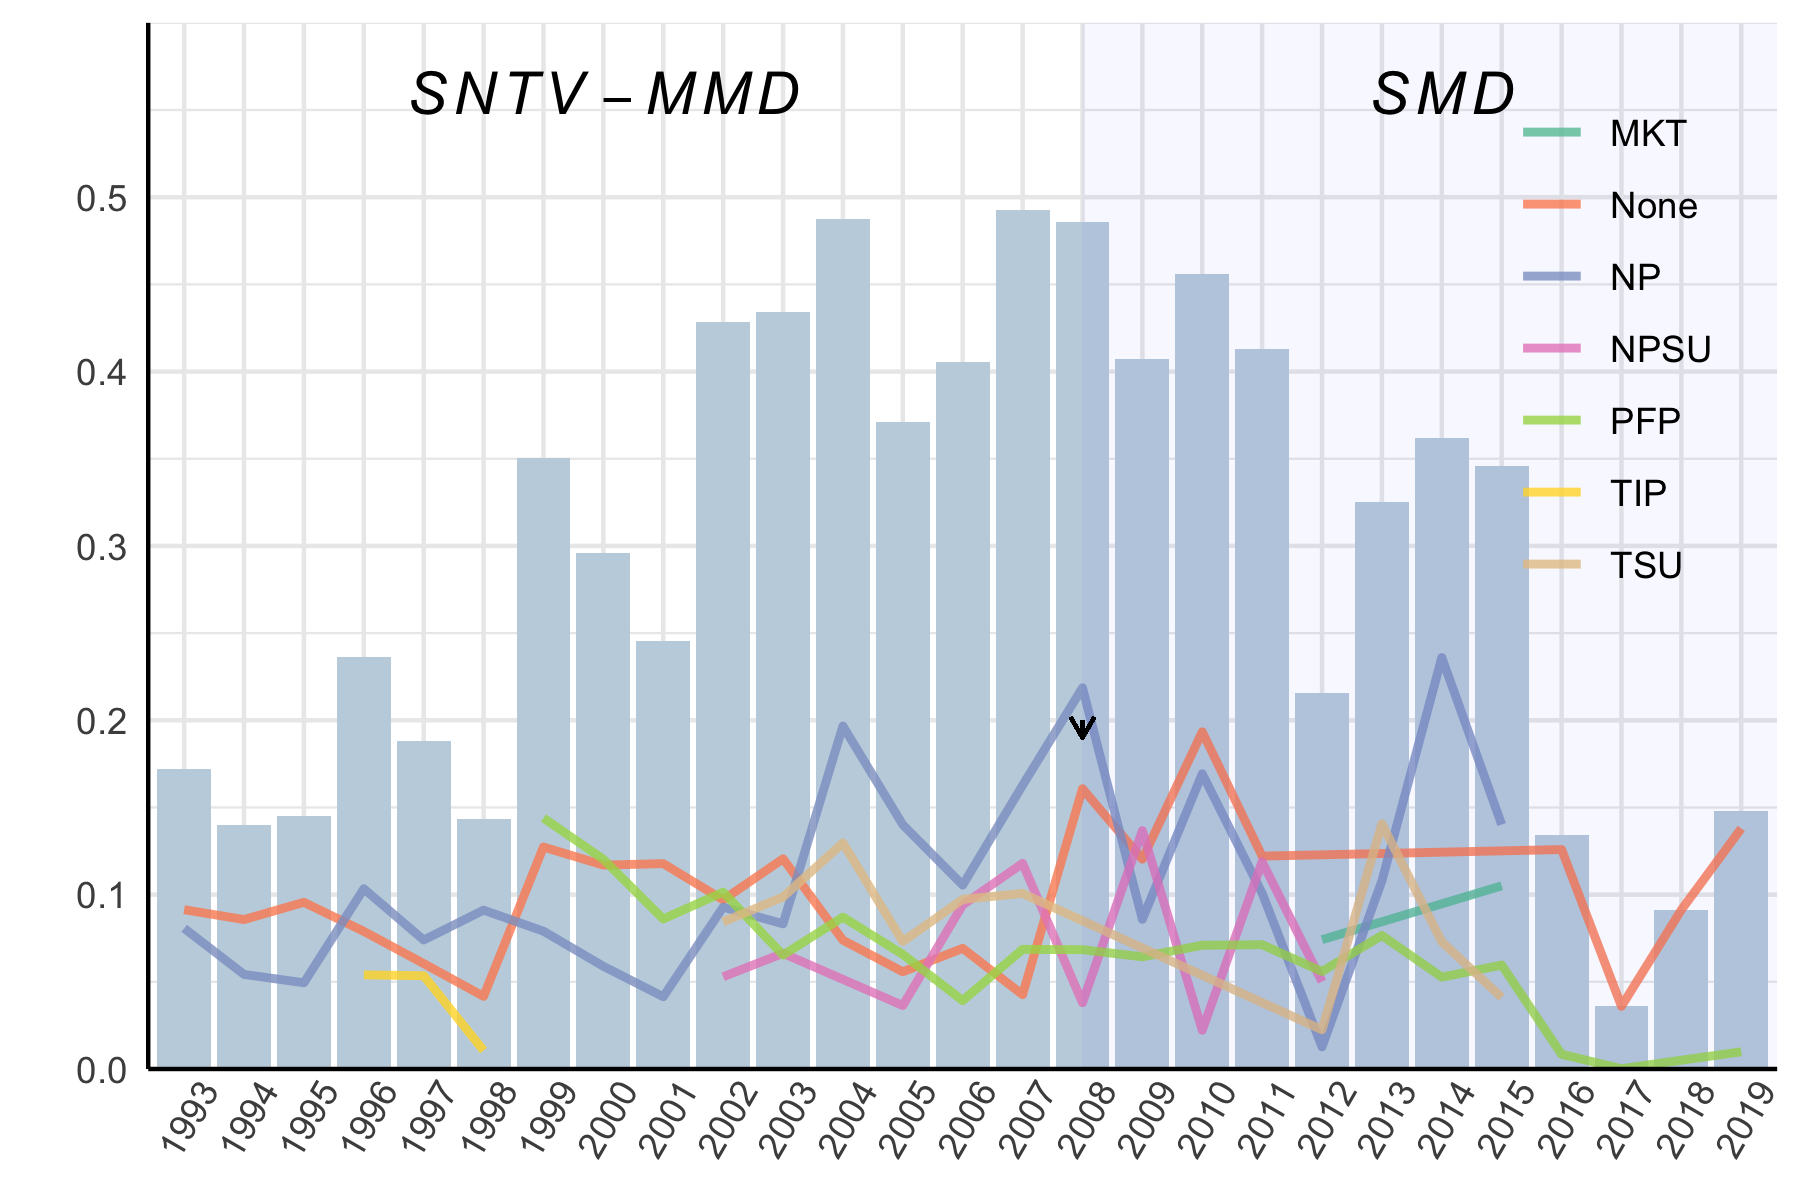
\includegraphics[width=7.2cm, height=6cm]{03-Chapter-Three/image/smallpqmean.png}
    \caption{Small Parties}
    \label{fig:meanporksmall}    
    \end{subfigure}
    \caption{The Mean Number of Pork Barrel Question by Years}
    \label{fig:meanpork}    
\end{figure}


\section*{\centering The Presence of the Electoral Reform}

How does the reform from SNTV-MMD to SMD-MMM change legislators' representation? To answer the question, I investigate to what extent the reform reduces legislators' incentive to ask pork-barrel questions. In total, legislators asked 116,248 questions throughout the reform transition from 1993 to 2020. While multiple plunges and surges between 2000 and 2015 reveal that the passage of years possibly affects the legislators' intention to propose the questions. To distinguish any irrelevant event to influence our analysis, I first calculated the mean of the pork features by an individual legislator at a quarterly unit and ran the following regression in \autoref{eqn:reg}, 

\begin{equation}
\begin{aligned}
 Pork_{i,t} = & \alpha_{0}+\alpha_{1}Electoral Reform_{t}+\alpha_{2t} +  \\
              & \alpha_{3}{(Electoral Reform_{t}\times{t})} +            \\
              & \theta C_{i,t}+ \epsilon_{it},
\label{eqn:reg}            
\end{aligned}
\end{equation}

where the dependent variable, $Pork_{i,t}$, is mean of pork-barrel questions aggregated at quarterly individual level, $ElectoralReformt_{t}$ is a dummy variable indicating whether the observation is  from the period of the post reform, $C_{i,t}$ includes fixed effects for municipality $i$ in election $t$, and $\epsilon_{it}$ is the error term. \autoref{tab:reg} shows a negative and significant effect on legislators' motivation to ask pork-barrel questions after reform, both for \textit{Full Model} and \textit{Large Parties}, suggesting that changing to SMD decreases legislators' incentives to pay attention to parochial interests. Thus, I find generally consistent empirical evidence in favour of \textbf{the Hypothesis \ref{h:h1}}. 

Yet, the heterogeneity issues resulting from natural disasters and political incidents occurred in years that could potentially influence legislators' incentive to ask specific questions or ask more (less) questions. For example, in 2006, a mass movement (\textit{Million Voices against Corruption, President Chen Must Go}) in Taipei Liberty Square led by former DPP Chairman Shih Ming-teh pressured President Chen Shui-bian to resign. This incident was in the media for more than a year, from 2007 to 2008, when the reform was just in practice. To diminish the problem concerning the heterogeneity, I control for the fixed effects from municipalities and legislators across the years. Still, the reform is statistically significant negative, and robust in models (2) and (4). 

As such, the empirical evidence shows that increases in time were associated with higher motivation levels to ask pork questions under the old system, SNTV-MMD, and lower levels under SMD. This suggests the institutional change reduces legislators' tendency to ask for the pork-barrel project between KMT and DPP, even if I introduce municipality dummies, legislator dummies, control for the passage of time and other demographics. 


\begin{sidewaystable}[!htbp]

% \begin{table}[h]
    \centering
    \caption{Regression Analysis for Pork-barrel Questions}
\scalebox{1}{
    \begin{threeparttable}
    \def\sym#1{\ifmmode^{#1}\else\(^{#1}\)\fi}
    \begin{tabular}{l*{6}{c}}
    \toprule 

                &\multicolumn{2}{c}{Full Observation} 
                &\multicolumn{2}{c}{Large Parties}
                &\multicolumn{2}{c}{Small Parties}\\
                 \cline{2-7}  \\
                &\multicolumn{1}{c}{Model  (1)}
                &\multicolumn{1}{c}{Model  (2)}
                &\multicolumn{1}{c}{Model  (3)}
                &\multicolumn{1}{c}{Model  (4)}
                &\multicolumn{1}{c}{Model  (5)}
                &\multicolumn{1}{c}{Model  (6)}\\                
                &\multicolumn{1}{c}{Interaction}
                &\multicolumn{1}{c}{+ Controls}
                &\multicolumn{1}{c}{Interaction}
                &\multicolumn{1}{c}{(+ Controls)}
                &\multicolumn{1}{c}{Interaction}
                &\multicolumn{1}{c}{(+ Controls)}\\
     \midrule


Reform          &  -14.052\sym{***}   &   -13.125\sym{***} 
                &  -14.959\sym{***}   &   -16.346\sym{***} 
                &  -11.180            &   4.954         \\
                &   (3.946)           &   ( 5.085)          
                &   (4.173)           &   ( 5.569) 
                &   (8.365)           &   (19.928)          \\


Year            &    -.006\sym{***}   &    -.006\sym{***}
                &    -.006\sym{***}   &    -.008\sym{***} 
                &    -.002            &    -.001             \\
                &     (0.001)         &    (0.001)     
                &     (0.001)         &    (0.001) 
                &     (0.002)         &    (0.003)            \\
                
Reform $\times$ Year   &    .006\sym{***}    &    .006\sym{***}
                &    .007\sym{***}    &    .008\sym{***} 
                &    .005             &   -.002                    \\
                &     (0.001)         &   (0.002)     
                &     (0.002)         &   (0.002) 
                &     (0.004)         &   (0.009)         \\

Constant        &   12.610\sym{***}   &    12.713\sym{***} 
                &   13.732\sym{***}   &    16.206\sym{***} 
                &    5.091            &     2.712          \\
                
                &   (2.129)           &   (2.735)          
                &   (2.408)           &   (3.672) 
                &   (5.614)           &   (6.546)          \\

     \midrule

District Fixed Effects&                     &   \checkmark         
                      &                     &   \checkmark   
                      &                     &   \checkmark      \\    
                     
Legislator Fixed Effects             &                     &   \checkmark         
                     &                     &   \checkmark   
                     &                     &   \checkmark      \\   
                     
The Reform Year      &    \checkmark      &   \checkmark         
                     &      \checkmark   &   \checkmark   
                     &    \checkmark         &   \checkmark      \\   
                     
Observations         &    4,252            &    4,252         
                     &    3,539            &    3,539
                     &    713              &    713        \\
Adjusted \(R^{2}\)   &    0.016         &    0.218
                     &    0.020         &    0.233   
                     &    0.003         &    0.179     \\
\bottomrule
\end{tabular}
     \begin{tablenotes}
     Note: * \(p<0.10\),** \(p<0.05\), *** \(p<0.01\). \\ Robust standard errors in parentheses. The district-level pork-barrel parliamentary question at quarter-yearly is regressed on year, electoral reform, and interaction between year and electoral reform, with and without fixed effect controls. The controls include fixed effects for electoral districts, municipalities, and individual legislators and the occurrence of the reform. 
     \end{tablenotes}
     \end{threeparttable}
     }\label{tab:reg}
% \end{table}
\end{sidewaystable}


To distinguish any possible effects from the passage of time and control for differences between municipality and legislators, I ran the same regression as above by using a subsample only including the large parties (KMT and DPP) and small parties. However, the presence of the reform has an insignificant impact on legislators from \textit{small parties}, revealing that the effects of institutional change do not substantively discourage most small-party members from asking pork questions. Under the SMD, the minority legislators were squeezed for living space in the legislature, which subsequently motivated them to make more efforts to appeal to parochial groups of voters and ask more pork-barrel questions to the government on behalf of their voters in the district. 

\section*{\centering Discussion}

This chapter contributes to the literature on electoral systems and political representation by demonstrating how the institutional change decrease legislators' incentive to run on their personal reputation by adopting electoral strategies that target the median voter. Combining a dedicated deep learning algorithm with robust regression analysis, I estimate the impacts of the electoral reform through SNTV-MMD to SMD on legislative behaviour. The results show that Taiwan's SMD diminishes legislators' motivation to mention pork-barrel features and increases their awareness of regulatory policies in written parliamentary questions. This finding is in line with a recent study by \citet{Catalinac2016, Ishima2020} showing that the single-member district system increases elected representatives' attention to national policies \citep{Catalinac2016}. Nevertheless, the institutional change has a moderate impact on legislators from smaller parties. This is due to the fact that the new system introduced in Taiwan is particularly disadvantageous to small parties \citep{Duverger1954, Reed2001, Huang2017, Bawn2003}, which deteriorates the effect of the reform on their political behaviours and electoral strategies with the constituencies. 

This chapter thus comes with some limitations. First, the fact that there has been a steady decrease in the total number of questions since 2003 despite the reform substantially impacting legislative representation is still noteworthy. In particular, social media in recent years has become an important platform for legislators to take positions and influence agenda setting \citep{Barbera2015, Barbera2019, Schurmann2022}. Additional limitations arise from the language transformation and its variation across times. As noted earlier in \autoref{sec:pqdata}, the pork barrel legislation from training data used in this chapter has been nearly ten years. The deep learning classifier learning patterns from the training set might fail to capture unknown concepts developed in the post-reform period. With BERT's self-attention mechanisms \citep{Vaswani2017}, the BERT-based framework may assist the machine classifier by simulating a similar skill set to human brains that can identify more complex or unseen concepts derived from the labelled data to understand the underlying pork barrel features.

Measuring legislators' preference towards constituencies under the different systems is essential to understanding the electoral system and the impacts on political representation. This chapter looks at an enduring myth about the impact of the 2008 electoral reforms in Taiwan. Although the reform, as scholars argue, some evidence indicates that SMDs may not be as effective as initially presumed in solving drawbacks of the SNTV, such as factional politics and intraparty competition \citep[e.g.,][ ]{Wu2003, Batto2018}. The empirical evidence shows that increases in time were associated with lower motivation levels to run on personal reputation despite the fact that intense conflicts between parties when the reform occurred \citep{liao2020}. 
%%%%%%%%%%%%%%%%%%%%%%%%%%%%%%%%%%%%%%%%%%%%%%%%%%%%%%%%%%%%%%
%%                 This is Chapter 4 (Paper 1)              %% 
%%%%%%%%%%%%%%%%%%%%%%%%%%%%%%%%%%%%%%%%%%%%%%%%%%%%%%%%%%%%%%
\chapter{Mayors and Pork Barrelling: Career Paths and Distributive Spending \label{chap:ch4}}
\clearpage
\section*{\centering Abstract}

\small The literature on distributive politics has provided several empirical pieces of evidence to explain how partisan bias and internal privileges in the legislature deteriorate government sources disproportionately allocated in villages or locations. In particular, the cause of pork-barrel allocation is typically explained by politicians\textquoteright rational calculation; their chances of staying in the office become higher if they can bring particularistic benefits to their targeted supporters. This chapter examines the contribution of the mayor's political career within governments in obtaining more distributive benefits for the municipality. Mayors with more sophisticated experience have stronger electoral ties to congress, which is useful for enhancing their chances of staying in office. Using the case of Taiwan and intergovernmental transfers allocated to each municipality, I find that municipalities whose mayors with longer careers spent in the legislature are more likely to be allocated higher fiscal expenditures. The effect is even more substantial if those legislators had previously been connected to the legislative standing committees. However, mayors' prior political career in ministries does not significantly help their municipalities obtain the grant. The findings suggest that, compared to experience as a central government official, a mayor with a legislative career significantly impacts the distribution of the transfers to municipalities.

\clearpage

\section*{\centering Introduction}
Most intergovernmental transfers are politically manipulated. Electoral incentives motivate incumbent legislators to bring pork barrel benefits to their home districts. The literature offers both theoretical and empirical explanations about how candidates' electoral incentives evolve in response to the different electoral systems \citep[][]{Myerson1993, Cox1990} and how electoral reform changes legislators' electoral strategies. In particular, after the electoral reform from the Multi-member Districts (MMD) to the Single Member Districts (SMD), legislators elected by SMD still actively engage in constituent service but shift to provide more services that target wilder median voters. For example, \citet[][]{Hirano2006, McKean2000} find that the distributions of particularistic benefits are found to be more concentrated in MMD than in SMD. While a plethora of work and discussion on the linkage of the electoral institution and legislators' representation, few empirical studies investigate possible factors caused by the reform that might deteriorate the inequality of government resources distributed to sub-national institution governments.

As \citet{Cain1987} and others note \citep[e.g.][]{Cox1987b}, parties had more success in appealing to the median voter with general interest policies than particularistic goods. For example, \citet{Cox1987b} studied Great Britain in the nineteenth century and found that interparty electoral competitions for general policy programs increased, and pork barrel policies declined as the districts enlarged during the 1830s and the 1880s \citep{Cox1987b}. \citet{Catalinac2016, Catalinac2017} finds that electoral reform through SNTV to SMD not only eliminated intraparty competition but also reduced Japan's Liberal Democratic Party candidates' incentive to promise pork barrel benefits to voters. The reform in Japan reduced LDP members' incentive to utilise \textit{Koenkai} (personal support groups, 後援會)  as well as a decreased need to spend money to maintain Koenkai and a personal vote \citep[][]{Carlson2006}. 

The literature on distributive politics has provided several empirical pieces of evidence to explain how partisan bias and internal privileges in the legislature deteriorate government sources disproportionately allocated in villages or locations across US. In particular, the cause of pork-barrel allocation is typically explained by politicians' rational calculation; their chances of staying in the office become higher if they can bring particularistic benefits to their targeted supporters. The conventional wisdom in the literature believes electoral incentives and the ability for elected legislators to secure the pork barrel benefits are motivated by several political factors, especially partisan bias and internal privileges, on distributive spending of all sorts. In Taiwan, intergovernmental transfers are not only essential to the development of local infrastructure (such as supporting local hospitals, fixing roads, and extending roads and train lines) but also politically manipulated by incumbent members who can make decisions about its appropriation.

Indeed, as expected by the theory \citep[e.g.][]{Lancaster1986}, candidates under SMD still have incentives to bring pork barrel spending to appeal to their supporters. However, enlarged districts and reduced electoral magnitudes made this strategy more costly and inefficient during the elections \citep[][]{Myerson1993, Cox1997, Carey1995}. In particular, adopting a single-member district strengthened the party leader's ability to discipline their candidates. Therefore, even though candidates want to woo their supporters, they still need to follow their own party's lead to not negatively affect the party's aggregate reputation \citep{Ramseyer1993, Hirano2006}.

Why do some of Taiwan\textquoteright s municipalities succeed in obtaining a larger share of intergovernmental transfers? Do those municipalities receiving higher particularistic benefits have more connections to the legislature? The evidence from both theoretical and empirical expectations suggests that candidates' electoral incentives evolve in response to the different electoral systems \citep[][]{Myerson1993, Cox1990}. In particular, after the electoral reform from the MMD to SMD, the intergovernmental transfer as a pork barrel with signalling purposes is no longer necessary for elected legislators to achieve electoral success. Theoretically, legislators elected by SMD are believed to engage in constituent services that target median voters than parochial supporters. However, in reality, most Taiwan intergovernmental transfers are politically motivated and disproportionately distributed across municipalities. 

To continue political careers after the reform with the concurrent effect of reduced seats, an increasing number of legislators started to run for municipal mayor election. Afterwards, some municipalities have more mayors with more experience and connection to the congress, and some do not. Thus, a municipality whose mayors are more well-connected with congress has an advantage in receiving government funds. While the electoral incentive of legislators and policy motivation of presidents are often viewed as contributing to the inequality of pork-barrel benefits, the mayor's sophistication of political connection with the central governments also impacts the allocation of such benefits. Therefore, this paper measures the mayor's prior career and political connections and tests the effect of different types of connection, e.g. ties to the central governments, including the congress. In particular, this paper explores whether a municipality whose mayor politically aligns with the central government has an advantage in allocating distributive spending. 

To measure the impact of the imbalance distribution of the grant distributed by the central government, I examine the relationship between mayors' prior years of experience in the Legislative and Executive Yuan and the amount of Revenue Support Grant that each local government receives from 2000 to 2018. Our empirical finding shows that mayors with longer political careers within the central government generally substantially impact the allocation of pork-barrel benefits to their municipalities. By further decomposing the mayor's experience, municipalities whose mayors with more years of experience in the legislature are more likely to be allocated more disproportionate transfers. The effect is even more substantial if those legislators had previously been connected to the standing committees. 

%The literature on distributive politics has provided several theoretical and empirical pieces of evidence to explain how and why legislators' internal privileges and electoral incentives impact government sources centrally allocated in villages or specific locations. Specifically, in the context of the legislative politics, the cause of pork-barrel allocation is typically explained by legislators\textquoteright{} rational calculation; their chances of staying in the office become higher if they can bring particularistic benefits to their targeted supporters. The incentives and the ability for elected legislators to secure the pork barrel benefits are thought to be influenced by such factors as electoral systems, party affiliation, electoral vulnerability, committee positions, seniority and policy goals made by president \citep[e.g,][]{Kriner2015,Batto2005, Luor2009, Luor2004, Luor2008, Wang2009,Wang2012}. The existing literature particularly highlights motivations and reasons that explain privileged legislators can gain more access to fiscal resources. This paper shows that mayors' previous political ties to the central government potentially influence resource allocation.

% However, Carey and Shugart (1995) pointed out that if there is intra-party competition, the greater the number of candidates from the same party in the constituency, the greater the emphasis on individual votes. In addition, Norris (2004) pointed out that the smaller the constituency, the more incentive for MPs to build individual votes.

% The literature has envisioned several reasons to explain the allocation of distributive benefits may vary. Specifically, in the context of the legislative politics, the cause of pork-barrel allocation is typically explained by legislators\textquoteright{} rational calculation; their chances of staying in the office become higher if they can bring particularistic benefits to their targeted supporters. The incentives and the ability for elected legislators to secure the pork barrel benefits are thought to be influenced by such factors as electoral systems, party affiliation, electoral vulnerability, committee positions, seniority and policy goals made by president \citep[e.g,][]{Kriner2015,Batto2005, Luor2009, Luor2004, Luor2008, Wang2009,Wang2012}. The existing literature particularly highlights motivations and reasons that explain privileged legislators can gain more access to fiscal resources. This paper shows that mayors' previous political ties to the central government potentially influence resource allocation.


\section*{\centering The Mayors and Their Prior Experience}
Can a mayor who has more connection to the central government receive higher particularistic goods? This article contributes to distributive politics in emerging democracies by focusing on the relationship between the attributes of the mayor and their connection to the central governments. The literature consistently identified differences and correlations between legislators' bill sponsor behaviour and the distribution of the pork barrel project. For example, an examination of bill sponsorship is studied to look at how elected legislators increase their chances of staying in office by promising the pork-barrel projects \citep{Luor2008,Luor2009,Luor2012,Sheng2014a,Sheng2014b}. While these measurements for assessing pork barrels have some limitations at the municipal level, the literature on Taiwan politics successfully finds that legislators with an internally privileged position are more likely to secure higher grants and use them strategically to enhance their prospects of winning the next election. 

The governmental resources distributed to the sub-national governments are an important electoral strategy for the ruling government and incumbent legislators to consolidate their electoral advantage against the opponents. The literature posits that elected legislators have incentives to maintain the margin of victory by providing particularised benefits to key constituencies and co-partisan strongholds politically aligned with themselves \citep{Calvo2004,Keefer2008,Keefer2009,Ravanilla2017,Fabre2017}. For example, \citet{Ravanilla2017} finds that elected legislators attempt to reinforce their electoral strength by strategically manipulating spending allocation in favour of co-partisan mayors, resulting in heterogeneous distributions of annual spending allocated across municipalities. Similarly, \citet{Fabre2017} finds that municipalities to which a minister was more political career-connected are likely to be distributed 45\% higher in the number of discretionary subsidies than those who have less connection. 

The mayors with longer years of experience as legislators are expected to have stronger communication skills to manage good relationships with ministerial officials. Therefore, such career experience assists the mayors in developing skills to cooperate with the current legislators elected by the same municipality and interact well with the business in the municipality. It is, therefore, not surprising that those mayors can get an edge over their opponents in receiving more intergovernmental transfers. In this paper, I argue that rather than being dominated by legislative factors, the distribution of pork-barrel projects is driven by a group of mayors who have more networks within the governments. Therefore, their municipalities are likely to attain more fiscal resources. 

In Taiwan, the number of municipalities whose mayors formerly served as central government officials have been steadily increasing over the years, as shown in \autoref{figure1}. Comparing the variation in a given year, a gradual increase in the total number of municipalities whose mayors formerly served as a legislator has increased threefold since 2000. In particular, a significant change arose after the electoral reform.\footnote{\autoref{figure1} displays years of experience the mayor has served in the central government across years. To break down, the top grey area in each bar represents a given year of the whole municipalities whose mayors formerly served as legislators, and the dark bottom area represents years of experience mayors who formerly served as ministers in a given year. For example, the upper bar of 2005 is 80 years of experience; total mayors have served as legislators, and 19 years of experience mayors have had a position as ministers in 2005. The left-hand-side shaded area covering the year 2000 to the year 2007 indicates the period of the Single Non-transferable Vote (SNTV) in given those years, while the right-hand-side light area covering the year 2008 to the year 2017 reflects the period of the Single Member Districts (SMD).}

\begin{figure}[ht]
\begin{centering}
\caption{Mayors' Years of Experience in the Central Government\label{figure1}}
\par\end{centering}
\centering{}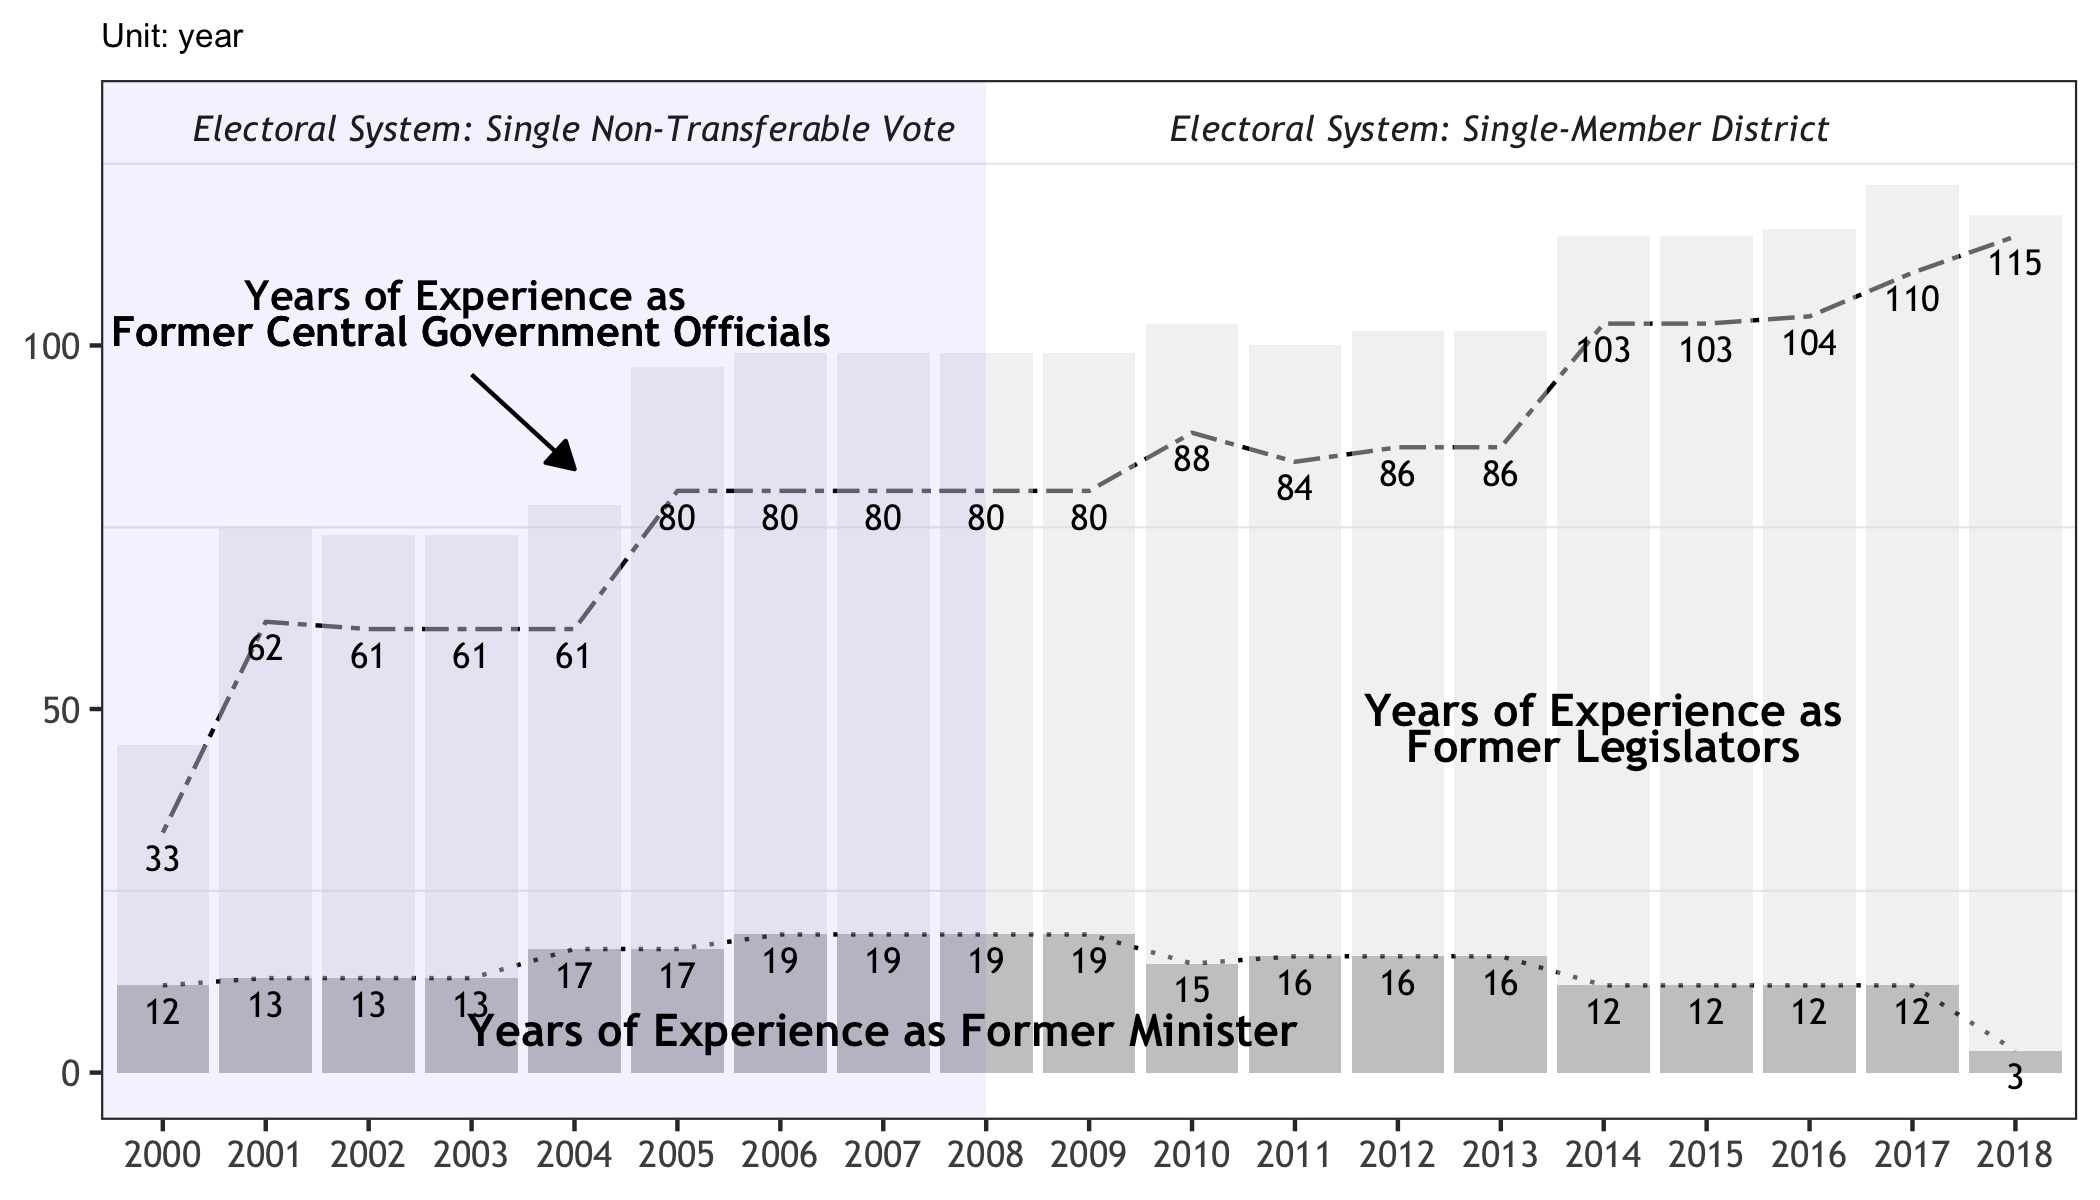
\includegraphics[scale=0.18]{04-Chapter-Four/image/figure1.jpeg}
\end{figure}

\section*{\centering Intergovernmental Transfers and Municipalities}
The municipal government in Taiwan is managed by a mayor elected with a four-year term by the people living in the municipality. Except for the special cities, mayors can continuously be in office if successfully re-elected, which increases incentives for mayors to secure more grant transfers to their municipality. As shown in \autoref{figure2}, the distributions of revenue types point out that approximately more than 40\% of local governments per year rely heavily on the revenue support grant to assist their fiscal expenditure. To secure higher grants, mayors are motivated to seek maximum expenditures. They not only propose projects that fulfil the criteria of receiving grants regulated by the Executive Yuan (the executive branch)  but also reach out to the legislators in an attempt to influence the budgetary decisions. 

Meanwhile, the grant allocation is not distributed following a demographic formula, as the trend varies and frequently fluctuates over time.\footnote{The revenue support grant is discretionarily allocated to municipalities to balance fiscal disparity among the municipalities. Initially aiming for the facilitation of efficient collaborations between inter-government during the development of public infrastructures and designed to be evenly distributed among governments, this grant in practice can be disproportionately distributed among local governments, possibly for specific reasons, such as a closer tie between local governments and the Executive Yuan. These factors have allowed mayors, who have more networks with cabinet officials, to gain privileged access to pork barrels from the central government.} \autoref{figure3} shows the annual distribution of detrended revenue support grants across years, eliminating chronological bias stemming from time-related trends. The enormous variation across all periods reflects that the fiscal revenue allocated by the Executive Yuan is potentially affected by multiple unexplained factors. These patterns ultimately reflected that the grant could be disproportionately more allocated to some municipalities, which the central government's distributive policies favour. 

\begin{figure}[ht]
\begin{centering}
\caption{The Proportions of Fiscal Resources Received by Municipalities\label{figure2}}
\par\end{centering}
\centering{}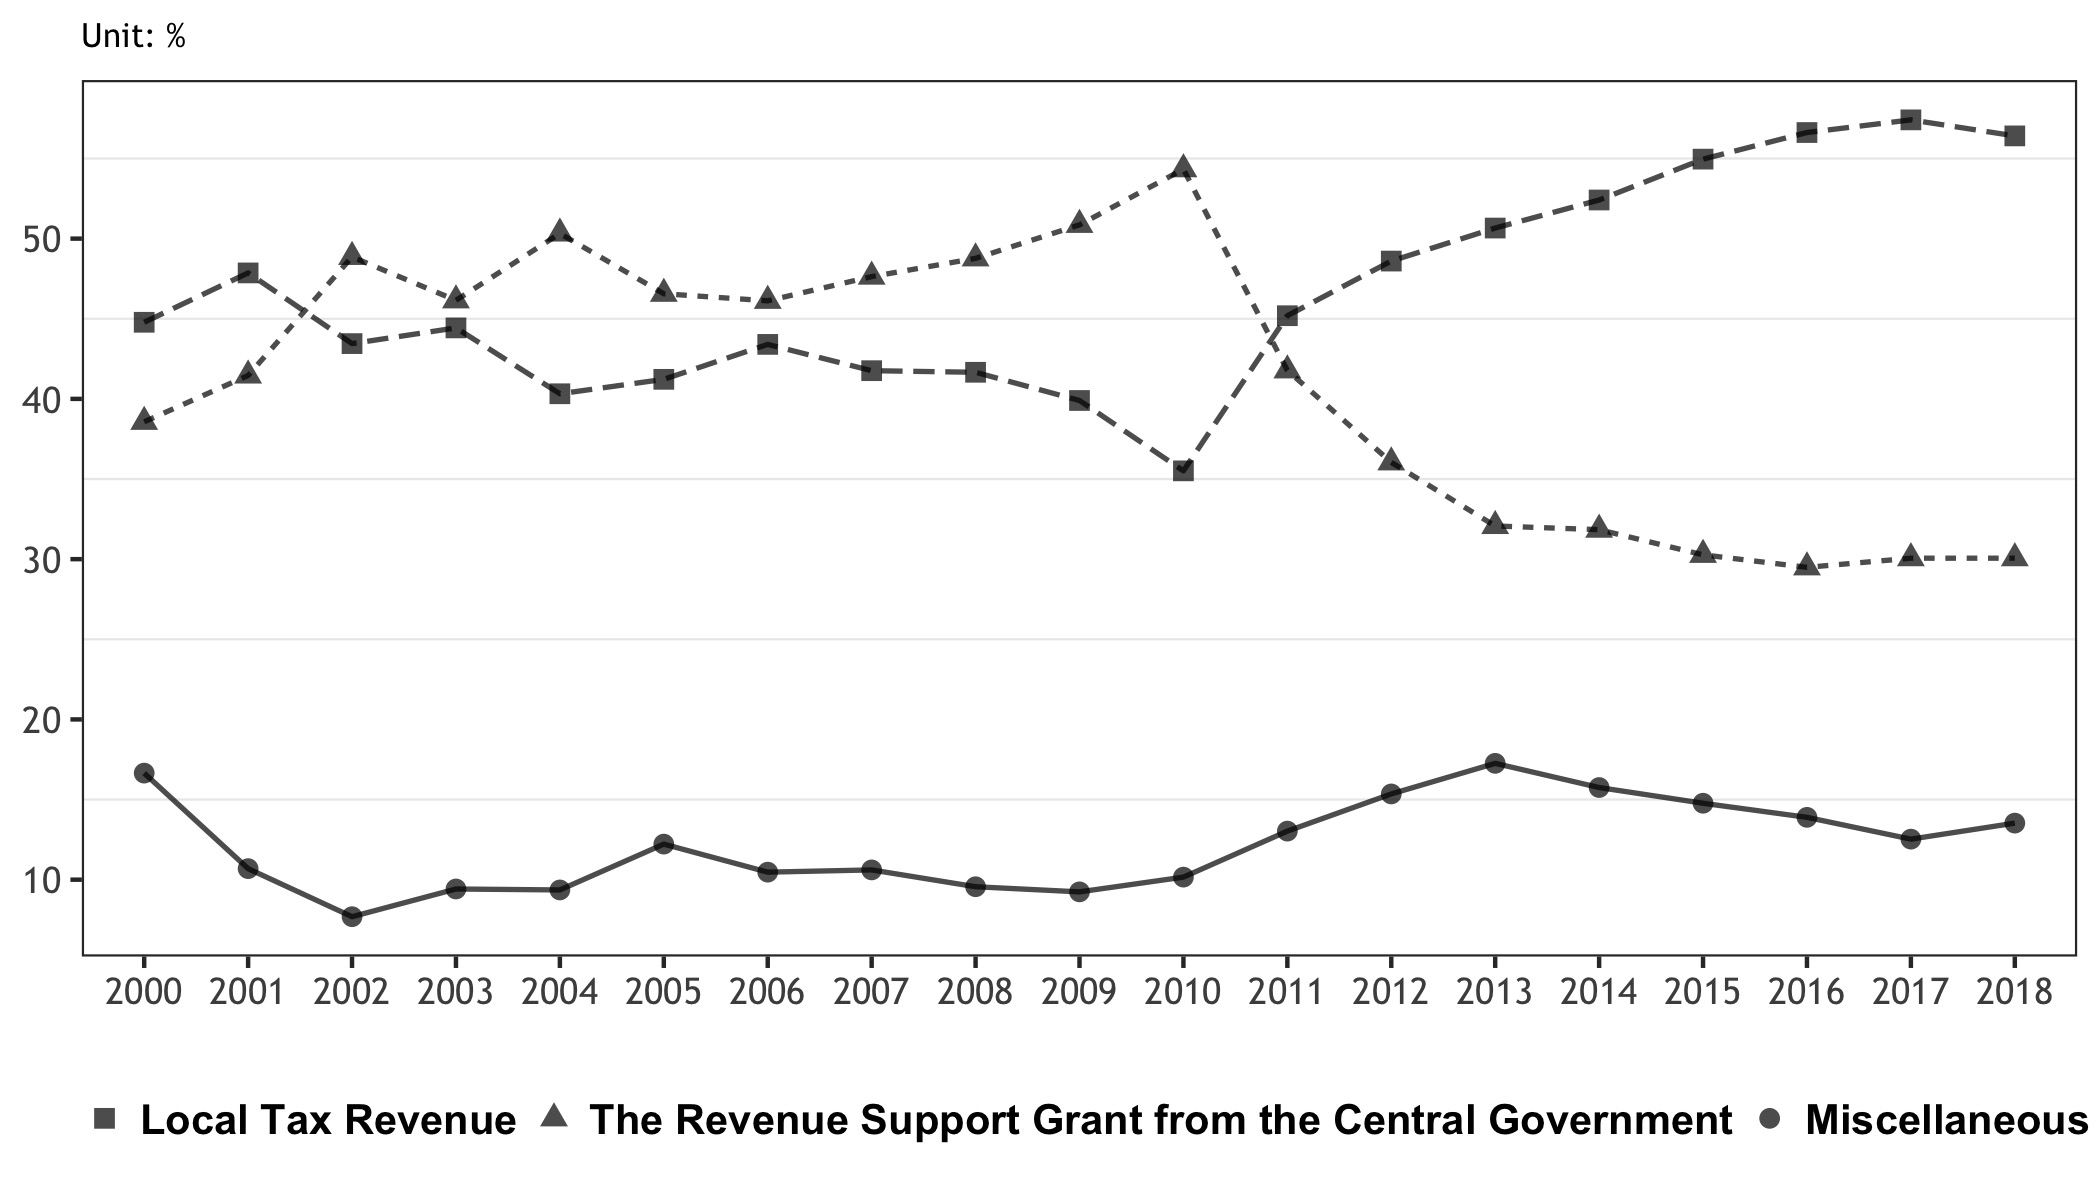
\includegraphics[scale=0.18]{04-Chapter-Four/image/figure2.jpeg}
\end{figure}

Moreover, revenue support grants also can be directly applied to finance the investment and maintenance of local infrastructures, such as public construction and urban development. For example, a municipality's expenditure on bridge and highway reconstruction is self-governed. Unlike other forms of grants, on the one hand, the granter of revenue support grant, the Executive Yuan, is not strictly obliged to obey a specific formula when determining the amount of grant allocated to each municipality. On the other hand, recipient municipalities can unconditionally dictate the money independently. 

\begin{figure}[!htbp]
\begin{centering}
\caption{The Annual Variation of the Detrended Revenue Support Grant\label{figure3}}
\par\end{centering}
\centering{}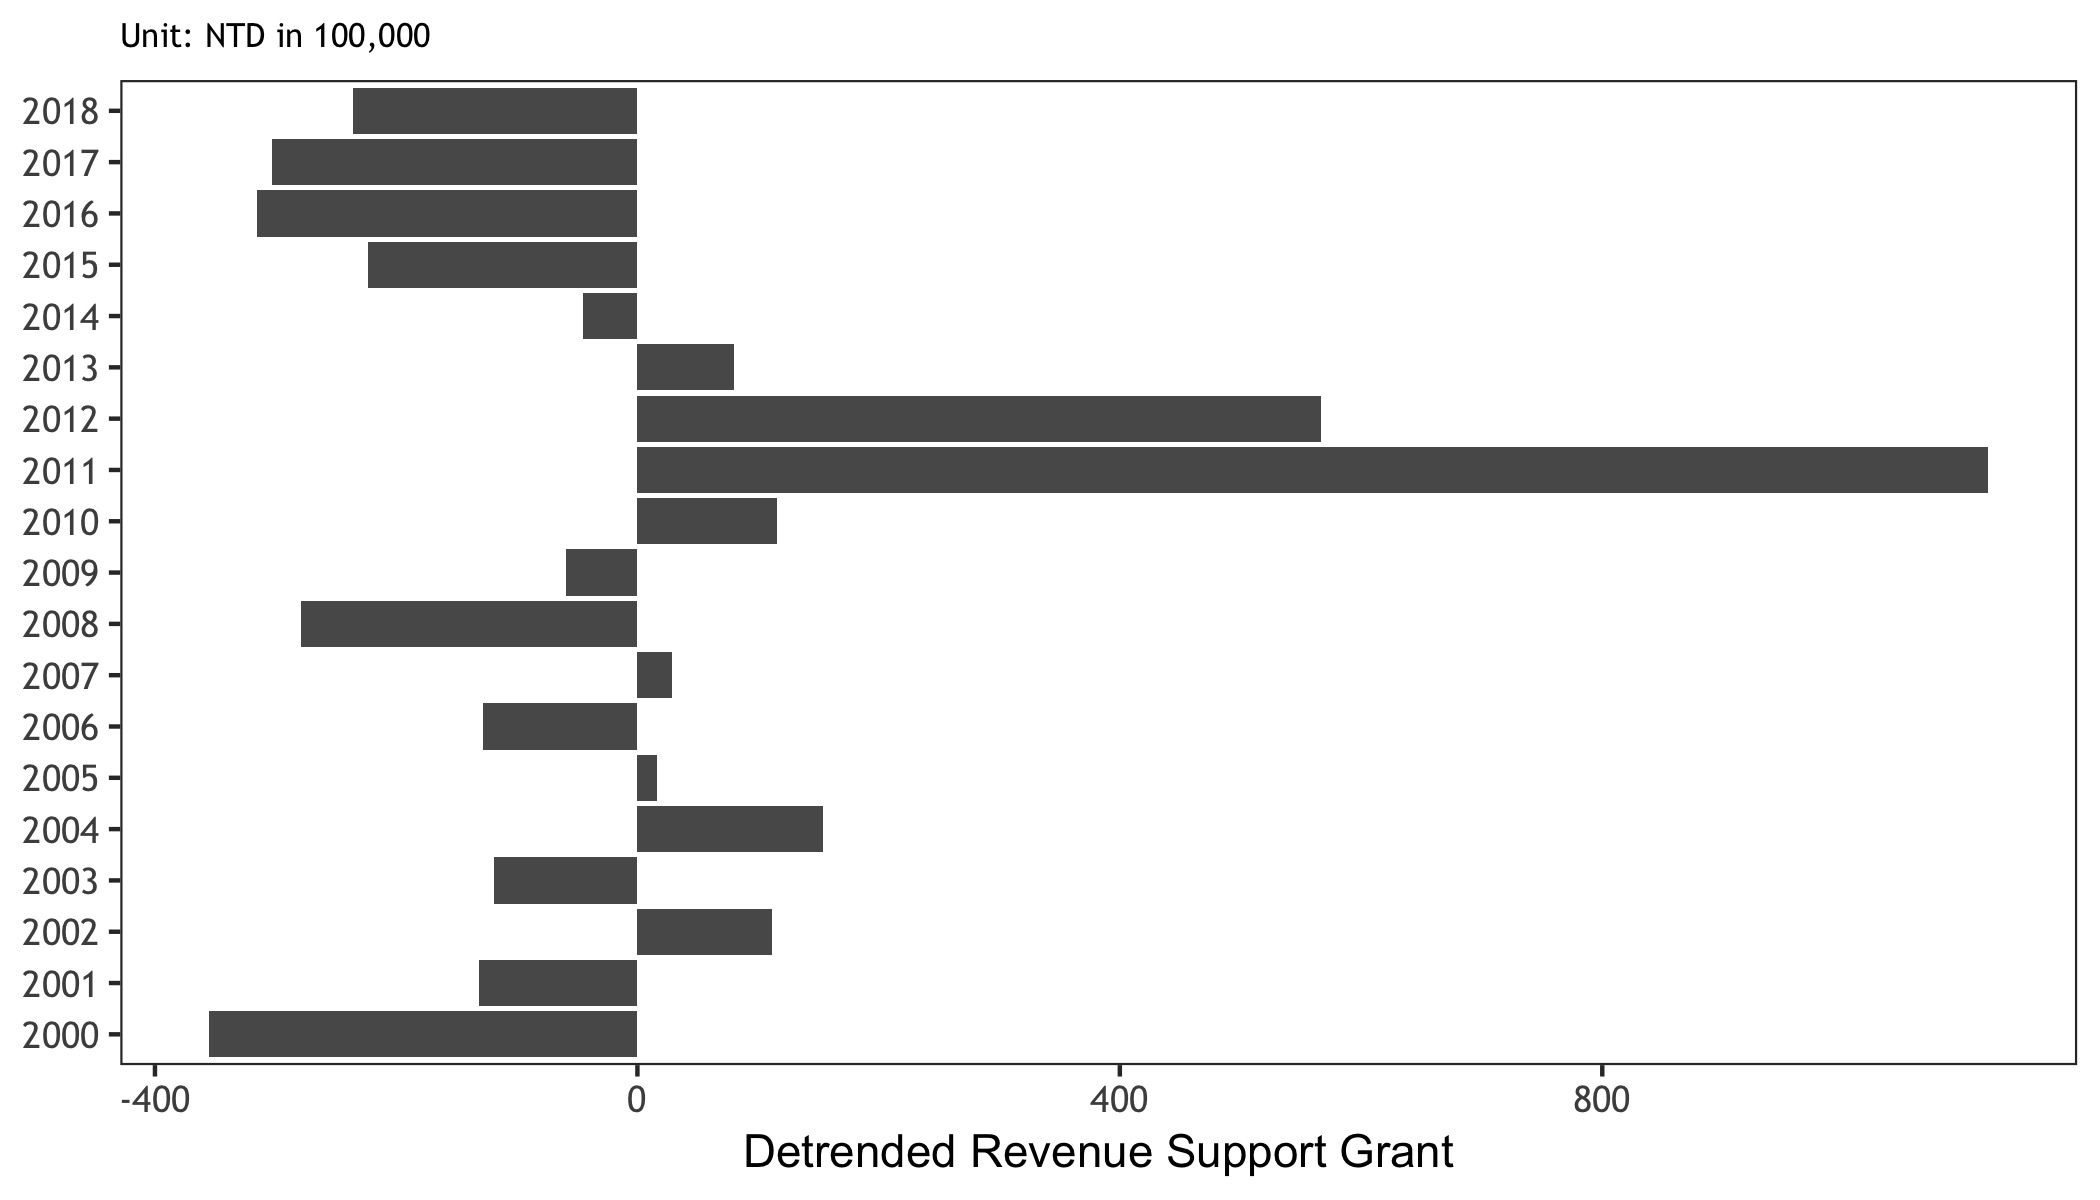
\includegraphics[scale=0.18]{04-Chapter-Four/image/figure3.jpeg}
\end{figure}


\begin{sidewaysfigure}[!htbp]
    \centering
    \begin{subfigure}[t]{0.48\textwidth}
    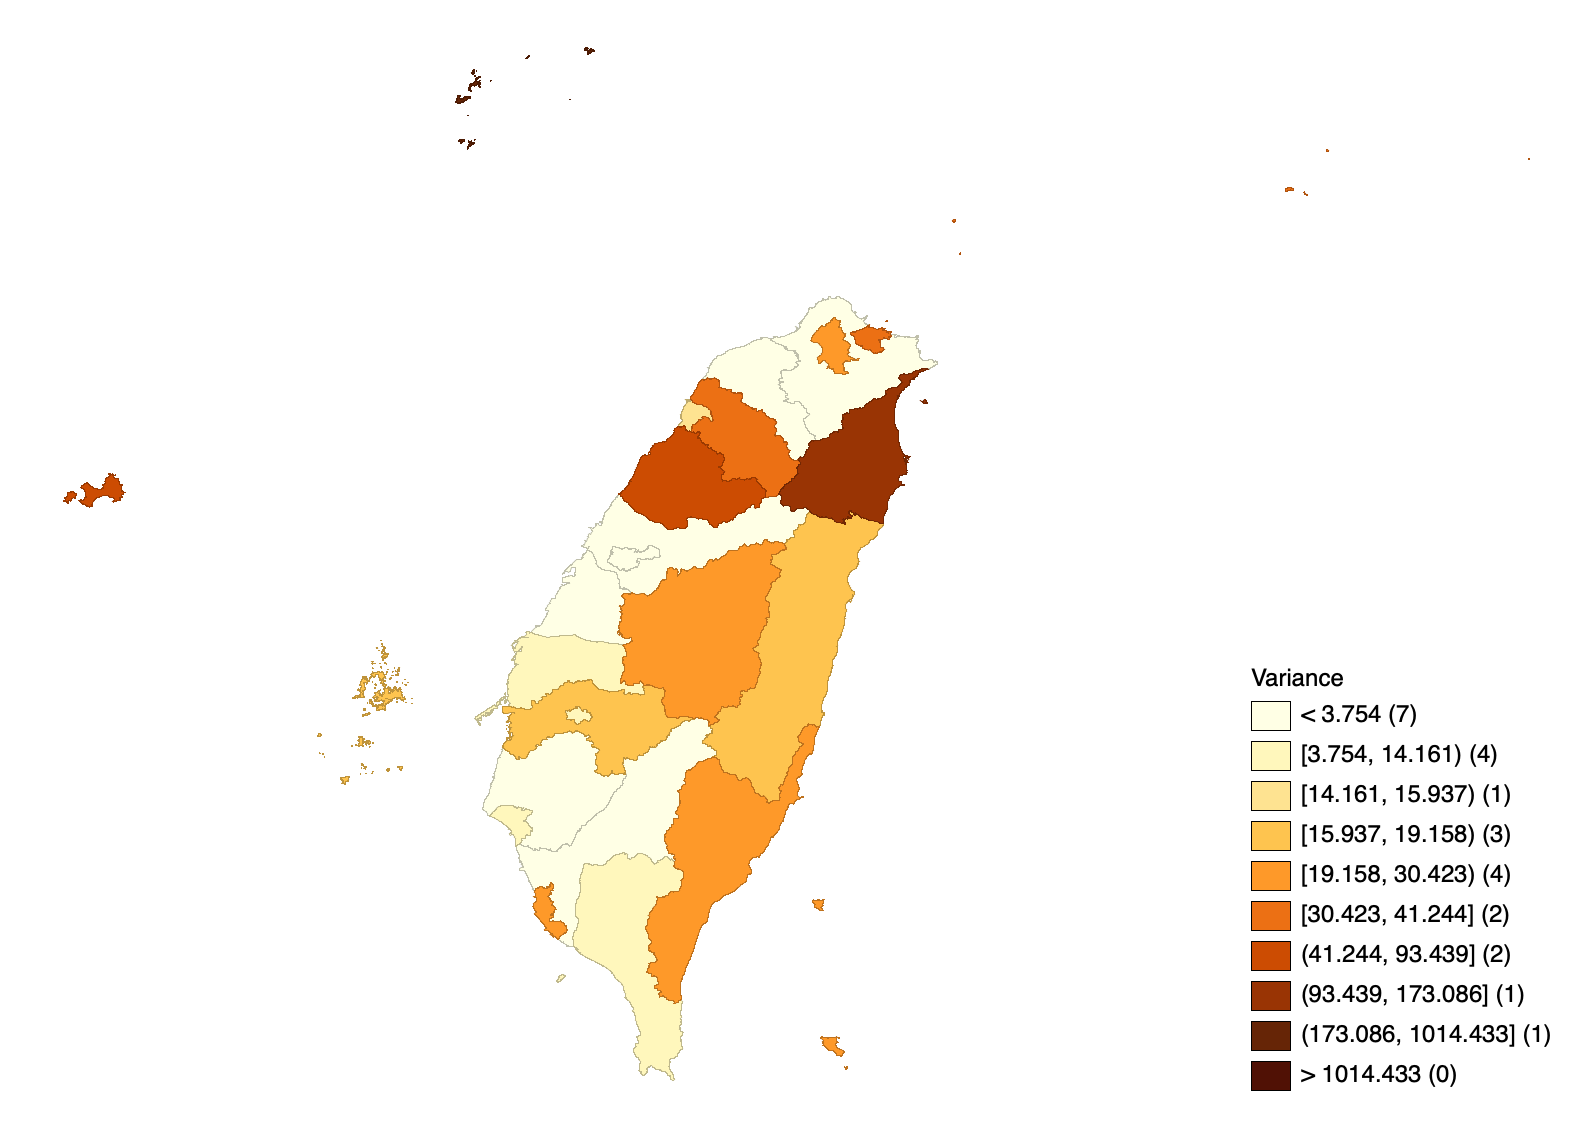
\includegraphics[width=7cm, height=6cm]{04-Chapter-Four/image/figure4-1.png}
    \caption{variance, \textit{pre}-refrom  \\ (No. of municipalities: 25)}
    \label{fig:figure4-1}    
    \end{subfigure}    
    \begin{subfigure}[t]{0.48\textwidth}
    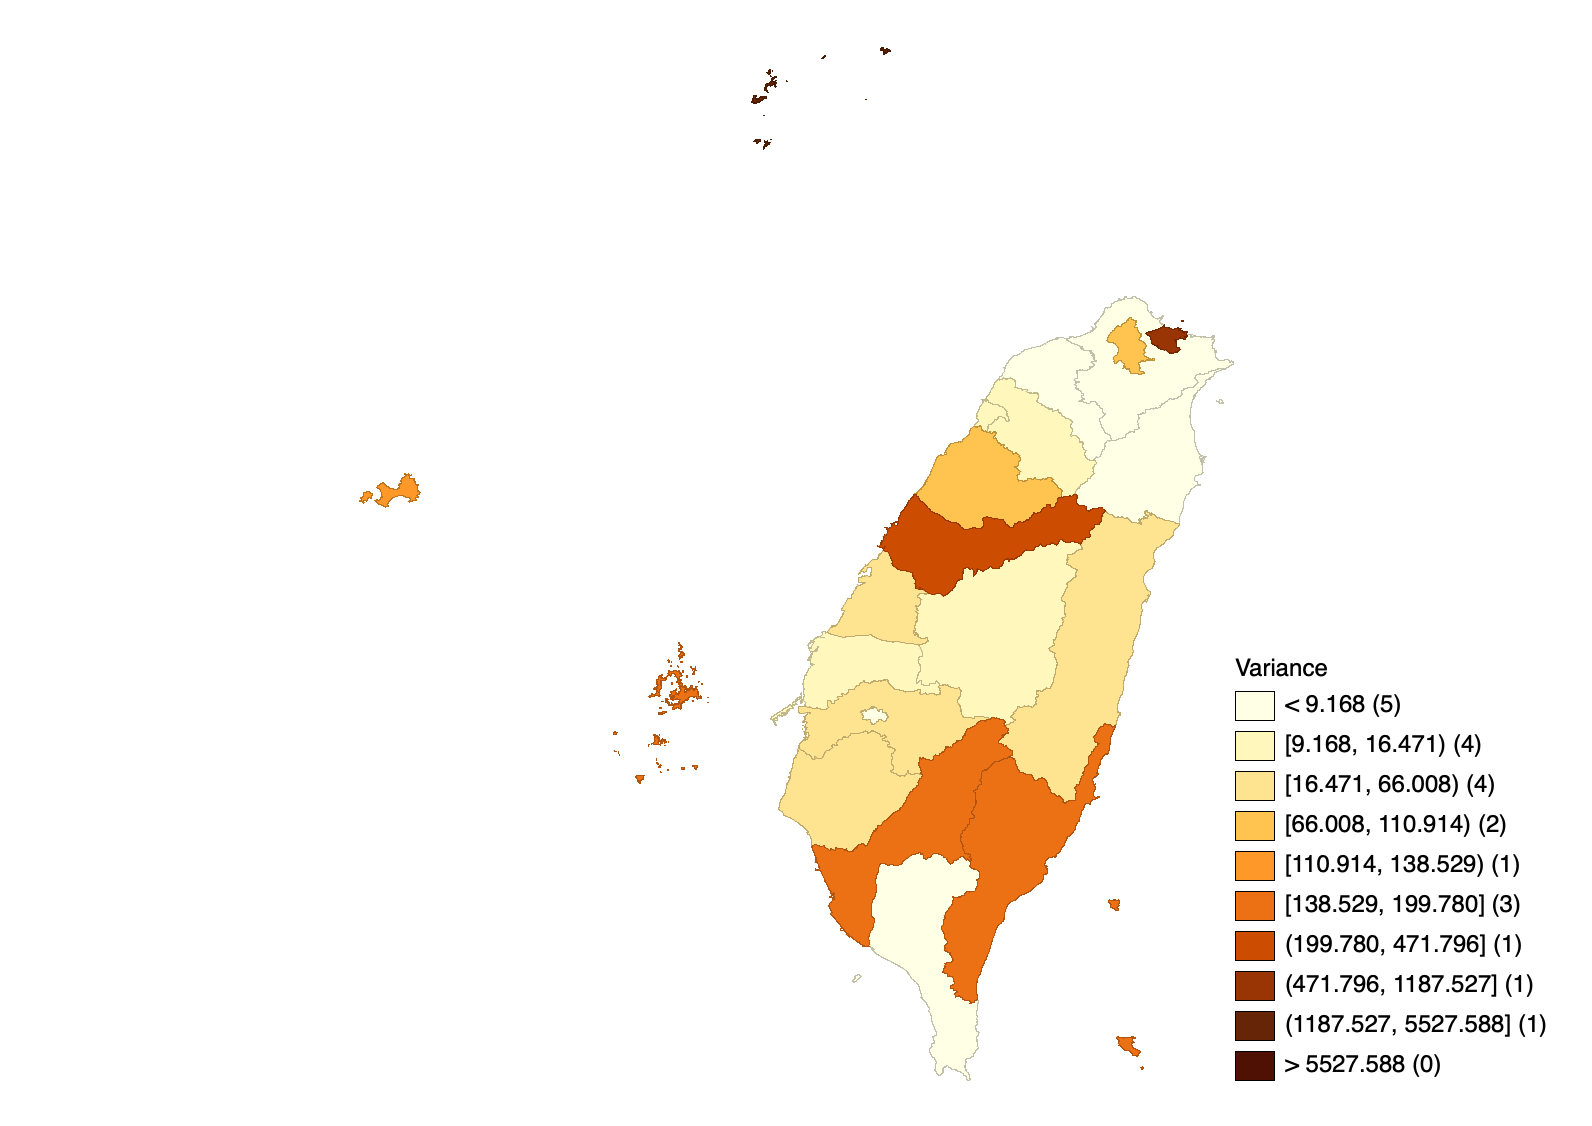
\includegraphics[width=7cm, height=6cm]{04-Chapter-Four/image/figure4-2.png}
    \caption{variance, \textit{post}-refrom \\ (No. of municipalities: 22)} 
    \label{fig:figure4-2}
    \end{subfigure}
    \centering
    \begin{subfigure}[t]{0.48\textwidth}
    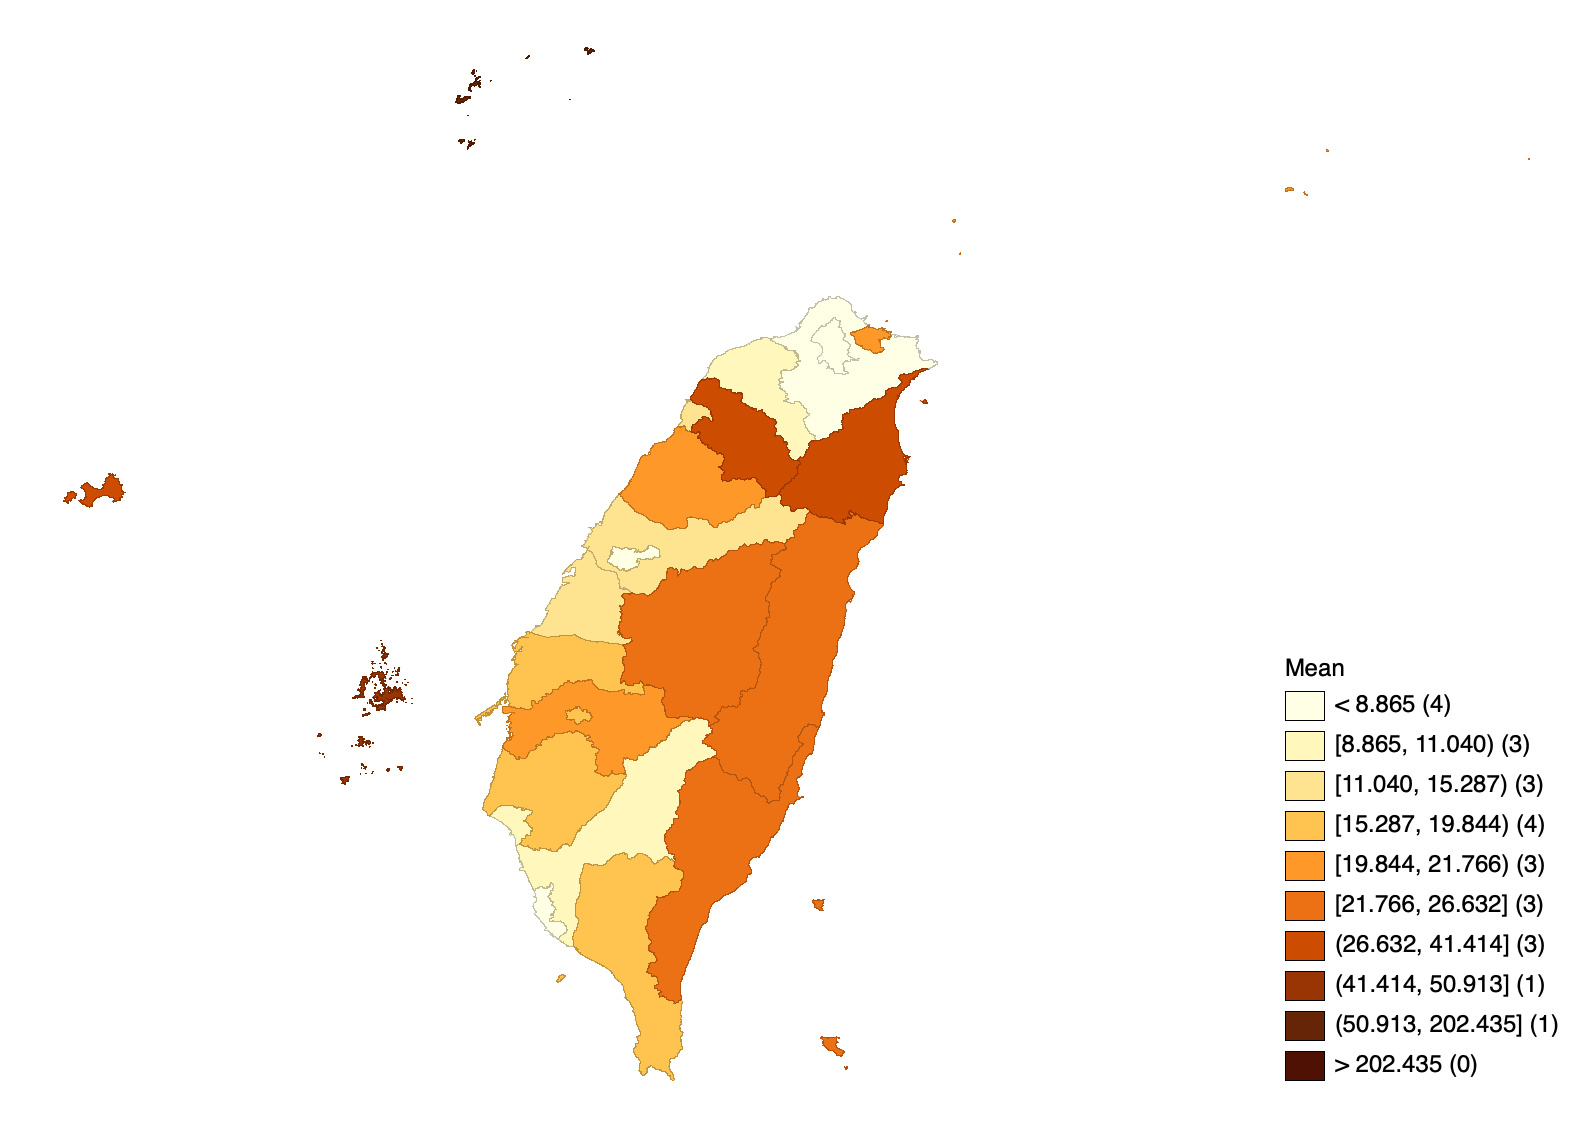
\includegraphics[width=7cm, height=6cm]{04-Chapter-Four/image/figure4-3.png}
    \caption{mean, \textit{pre}-refrom\\ (No. of municipalities: 25)} 
    \label{fig:figure4-3}
    \end{subfigure}    
    \centering
    \begin{subfigure}[t]{0.48\textwidth}
    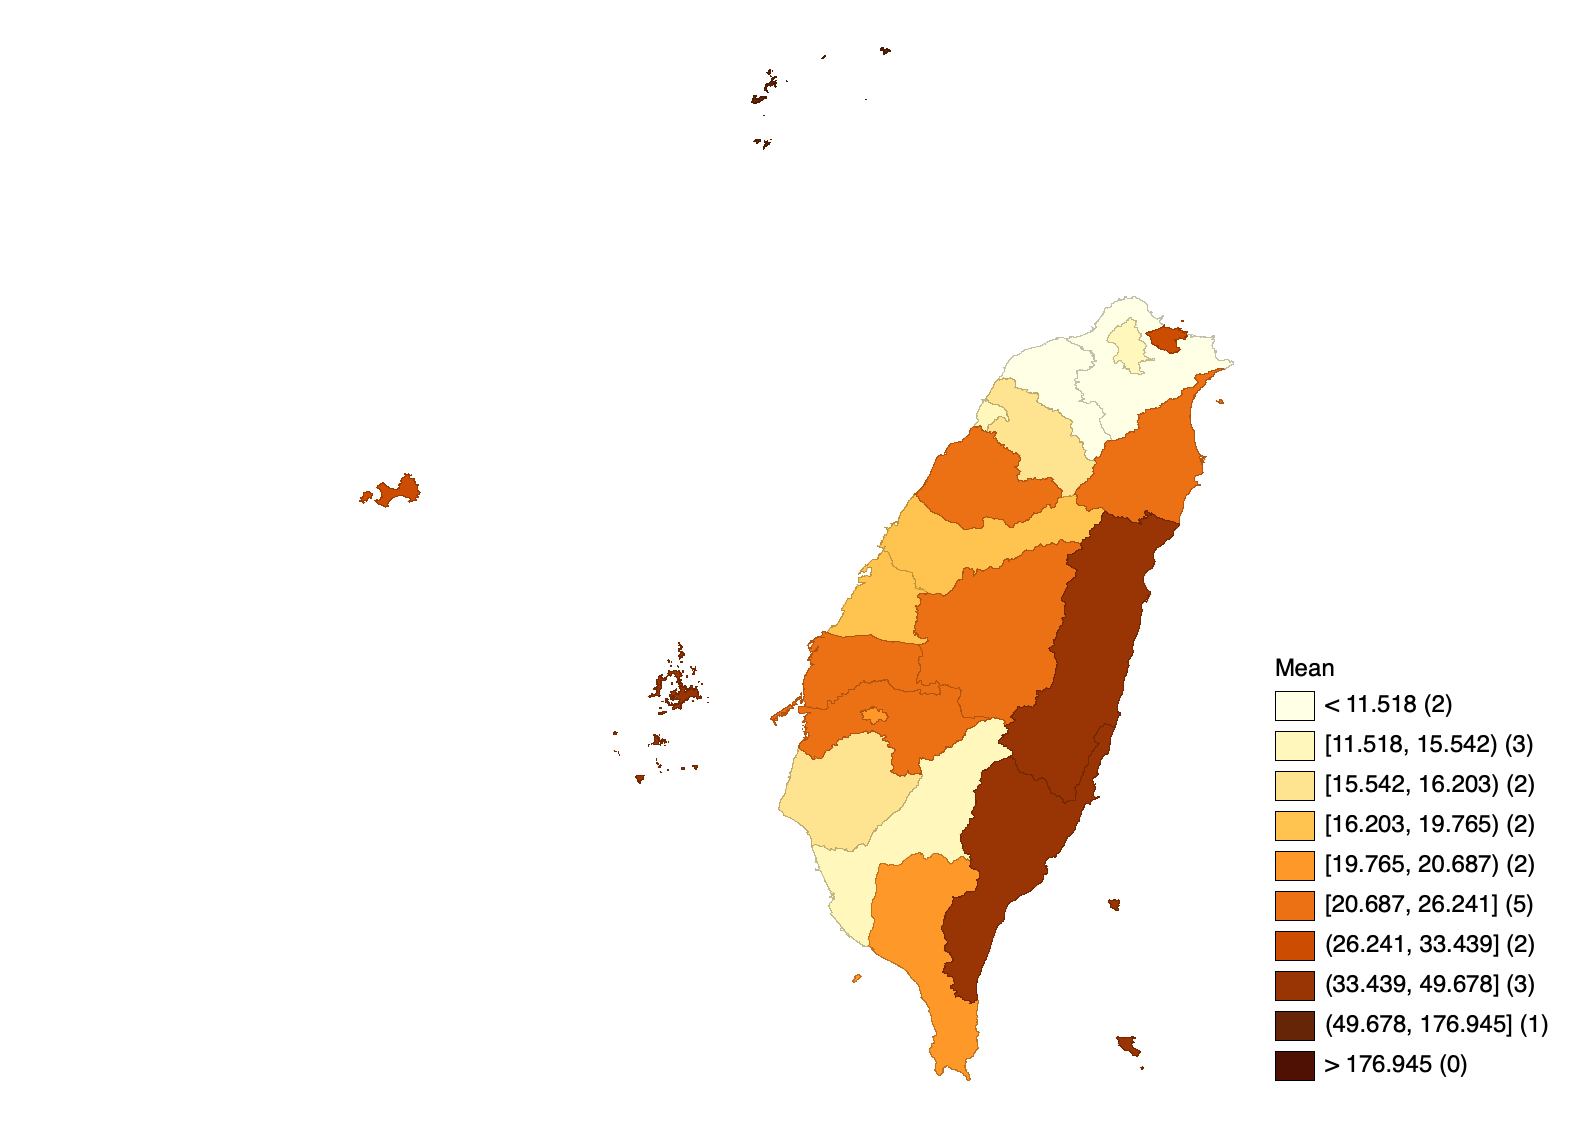
\includegraphics[width=7cm, height=6cm]{04-Chapter-Four/image/figure4-4.png}
    \caption{mean, \textit{post}-refrom \\ (No. of municipalities: 22)} 
    \label{fig:figure4-4}
    \end{subfigure}
    \caption{The Geographical Distribution of the Intergovernmental Transfers, Comparison between Pre- and Post-Reform}\label{figure4} 
\end{sidewaysfigure}

By visualising the patterns of the transfer distribution across municipalities, \autoref{figure4} describes variance and mean variations of the grant allocations per capita within each municipality. \autoref{fig:figure4-1} and \ref{fig:figure4-2} display the variance in grants distributed to each municipality over 2000-2008 (pre-reform) and 2009-2018 (post-reform). The deeper colour represents higher variation in the distribution of the grant. Similarly, \ref{fig:figure4-3} and \autoref{fig:figure4-4} show the average grant distribution allocated to each municipality. In particular, I observe a higher centrality within mid-eastern municipalities. For example, mid-eastern Taiwan always received higher grants, regardless of the merger scheme. According to these patterns, the ruling government potentially allocate to specific municipalities whose mayors are more politically associated with the central government. 

\section*{\centering Research Design}

\subsection*{Data}
To investigate whether mayors exploit their privilege of being aligned with the government party to obtain more grants, I identify each mayor's years of working experience within the congress (the Legislative Yuan) and the executive administration  (the Executive Yuan), and the amount of Revenue Support Grant that each municipal government allocated from 2000-2018.\footnote{The data are obtained from the Directorate General of Budget, Accounting and Statistics, DGBAS. The variables of interest are annually collected at the municipal level, which consists of the percentage of corresponding municipal mayors who previously served in the cabinet, the percentage of mayors formerly elected as legislators and representing the municipality, and whether mayors were once serving as a committee member in the Legislative Yuan. The data set contains each mayor's name and party affiliation, local demographics, and voter turnouts in presidential and mayoral elections (from the Central Election Commission, CEC). The control variables include the unemployment rate (from the Directorate General of Budget, Accounting and Statistics, DGBAS) and demographic information (from National Statistics).} In order to get accurate information regarding mayors' demographics, the data were cross-referenced by corresponding information on Wikipedia, local newspapers, municipalities' websites and the mayor's blog.

In my identification strategy, all ministries, councils and commissions are being comprehensively classified, except for ministers without portfolio who do not actually supervise any particular part of the cabinet in the central government.\footnote{The Executive Yuan, led by a premier and a vice-premier, comprises cabinet ministers (and its vice-ministers) and chairpersons of various councils (and its vice-chairpersons), and several (5-7 seats) ministers without portfolio. The premier (also known as the prime minister) appointed by the president requires no consent of the Legislative Yuan, while the president of the Republic appoints the vice premier and other members in the cabinet upon the recommendation of the premier. In addition to supervising the subordinate organs of the Executive Yuan, the premier must explain administrative policies and report significant policy changes to the Legislative Yuan.} As for the Legislative Yuan, its legislative seats comprise constituency seats that represent the people who live in the municipality, party-list seats that represent various parties, and reserving seats for aboriginals. In the data collection, all legislative seats are considered because the legislature plays a vital role in examining legal bills, treaties, and any general budget proposed by the Executive Yuan.\footnote{The minister includes the Ministry of Interior, Ministry of Foreign Affairs, Ministry of National Defence, Ministry of Finance, Ministry of Education, Ministry of Justice, Ministry of Economic Affairs, Ministry of Transportation and Communications, Ministry of Transportation and Communications, Ministry of Health and Welfare, Ministry of Culture, and Ministry of Science and Technology. The councils and commissions include Agriculture Council, National Development Council, Mainland Affairs Council, Financial Supervisory Commission, Overseas Community Affairs Council, Veterans Affairs Council, Indigenous Peoples Council, Hakka Affairs Council, Public Construction Commission, the Atomic Energy Council, Council for Economic Planning and Development (merged by the National Development Council in 2014); and Research, Development and Evaluation Commission (merged by the National Development Council in 2014). In addition, Independent Regulatory Agencies are incorporated into the classification, such as the Central Bank, Environmental Protection Administration, National Palace Museum, and the Consumer Protection Committee (dissolved in the Executive Yuan as the department of consumer protection in 2012).} 


\subsection*{Operationalisation}

The central government attempts to target key municipalities politically or geographically aligned with the central government. An increasing number of municipalities whose mayors have more experience in the legislature are thought to be distributed higher intergovernmental transfers from the central government. The literature has found the interaction between the fiscal resources distributed to local governments and partisanship that explains what motivates the central government to distribute higher fiscal resources to co-partisan strongholds in India \citep{Keefer2008,Keefer2009}, Argentina and Chile (\citealt{Calvo2004,Luna2010}) and in Mexico (\citealt{Diaz-Cayeros2003,Costa-i-Font2003}).

Thus, electoral pressures encourage the executive government or presidents to be more responsive to constituencies whose legislators are politically aligned with the central government. For example, the federal government is more likely to distribute disproportionately more fiscal spending to electorally important strongholds, particularly those states which are currently presented by governors or legislators from the president's party \citep{Aidt2012, Albouy2013, Kriner2015}. To control for the additional effects transmitted from the president and the legislator's attributes, I include three control variables: (1) whether the mayor's party affiliation is co-partisan with the president (\textbf{co-partisan mayor}); (2) the margin of the victory in terms of vote shares, won by the president during elections (\textbf{\%pres. vote}); and (3) the percentage of a municipality's legislators from the president's party (\textbf{\%co-partisan legislators}).

Thus, the relationship between the geographical allocation of revenue support grants and municipalities' attributes may be interfered with by, for example, municipalities represented by privileged legislators who hold strong agenda-setting positions in the legislature \citep[e.g.,][]{Engstrom2010, Martin2014}. The literature has explained the relationship between members having institutional position and the distribution of particularistic benefits \citep{Lazarus2009,Lee2003,Clemens2015,Balla2002,Lai2013,Luor2004,Luor2000, Berry2010}. Similarly, a positive correlation was found Taiwan municipalities receive disproportionately more central government grants when a legislator has standing committee membership, particularly those who hold committee chairs in powerful committees \citep{Chiu2013,Hsiao2007,Matsuo2012,Lai2013}.

To control the influence of the privileged legislators, I introduce two dummy variables that indicate (1) committee chair status (\textbf{committee chair}) and (2) member in powerful committees (\textbf{power committee}); and the number of sessions that the legislator has served in the congress (\textbf{seniority}).\footnote{I calculate the average seniority, average committee chair, and power committee in each municipality. For example, the seniority of legislators from the same municipality is added up across all local legislators for each year and then divided by the total number of local legislators in the municipality} Because some of the municipal governments are special autonomous cities and are directly controlled by the central government, I include a dummy variable indicating if a municipality belongs to this category (\textbf{special cities}). At the macroeconomic level, the unemployment rate is a measurement of the economic condition of a municipality and, therefore, is potentially relevant to grant allocation (\textbf{\%unemployed)} \citep{Adler1997}.

As indicated above, the distribution of such grants is a feasible proxy for the distribution of particularized benefits because they are disproportionately allocated within different local governments. In the data collection, the revenue support grant is individually identified annually from 2000 to 2018 across all municipalities. \footnote{It is worth noting that Lienchiang, Kinmen and Penghu are excluded from the regression analysis because these municipalities are the least populated and are surrounded by islands near Mainland China. Their grant allocations might potentially follow a different rule. I conduct a series of robustness analyses to check the performance of the outcomes by adding these surrounded islands in the sample to the regression estimation, see \autoref{tab:Robustness-of-Empirical-1} and \autoref{tab:Robustness-of-Empirical-2} in the Appendix \ref{sec:robustness}.} In total, the panel data set is unbalanced with 367 municipality-year observations, which resulted from the dissolution of certain municipalities into their surrounding neighbourhoods during the period.\footnote{\autoref{tab:variable} describes an overview of the independent variable and control variables as well as  the definitions of each variables.}

\subsection*{Estimation Strategy}
The estimation strategy is based on the adoption of panel data methods to test the significance of the coefficient between current mayors who have more previous experience in central government and distributive benefits across the municipalities.\footnote{In regression tables, the estimation of Model (1) is the results for the pooled cross-sectional model which treats the panel data as random samples simply drawn from the whole population, regardless of years. Under the statistical assumption that municipality-specific effects for different years are constant and time-specific effects for different municipalities are also $IID$, the Model (3) and Model (4) show the results of the models using the Fixed Effects by specifying the disturbance term $ \mu_{it}$, municipality dummies and year dummies to capture fixed and time-varying effects, respectively. The municipality-effect estimators in columns 3 yield consistent estimates under the assumption that some municipalities may potentially have strong connections which increase the municipalities' possibility of being given such a good share of the grant from the central government. For example, municipalities having a higher proportion of senior legislators or legislator holding privileged positions in the committee get themselves a great bargaining position in budgetary allocation. Likewise, time-varying effects could also be an issue if, for example, poor municipal governments that have been suffering from higher unemployment rates intermittently for many years are likely to be allocated more grants than other municipal governments. In order to compare the potentially different results of the estimation, column 2 of the table also includes a Random Effect model to confirm the robustness of the findings, under a different assumption from the Fixed Effect model, that the municipality-specific effects for different years are $IID$, similarly, time-specific effects from different municipalities are also $IID$.} In equation (1), $mayor_{i,t}$, as one of variables of interest indicates the past experience of the $i-th$ local government's mayor has in the central government at time $t$. Theoretically, if a mayor has more relative experience in the central government, with respect to other mayors, the current, say at time $t$, local government is more likely to receive more grants from the central government, that is, the extra experience plays a part in helping the local government (i.e. mayor) obtain a higher sharing of pork barrel benefits in following year ${t+1}$. 

In light of the municipal merge scheme after the electoral reform during the sample period, the value of experience does not imply same level of competitiveness in applying for central governmental grants in different years. Due to a variation in the total number of local governments existing across time, $mayor_{i,t}$ is adjusted by its municipal numbers to penalise potential effects of the mayors' experience in comparison to another at a different time (year) with lesser numbers of municipalities. More specific, $mayor_{i,t}$ is calculated as years of the central government experience of $i-th$ mayor, with respect to the total number of local government at $t$: $\Sigma_{1}^{T=t}\epsilon_{iT}$/$N_t$, where $\epsilon_m{}_n$ is the cumulative absolute experience of $m-th$ mayor has at time $n$, and $N_t$ is the total number of local governments. Notably, only the experience as Executive Yuan minister and Legislative Yuan legislator is counted as central government experience.

Based on the notations described above, the general model can be expressed
as Model (1):

\begin{equation} \ensuremath{y_{i,t+1}^{grant}}=\ensuremath{\beta_{A}{\Delta mayors}_{i,t} + X_{i,t}\gamma + \alpha_{i} + \delta_{t} + \varepsilon_{i,t}},\end{equation}

where $y_{i,t+1}^{grant}$ is the (log of) Revenue Support Grant per capita in New Taiwan Dollars (thousand) allocated to the $i-th$ local government by the Executive Yuan for period $t+1$; $\Delta mayor_{i,t}$ is the explanatory variable of interest, as explained above; the row vector, $X_{i,t}$, contains control variables isolating various effects from the legislature, the president and its own demographics, with
a column of corresponding coefficients $\gamma$. 


\begin{table}[!htbp]
\caption{The Estimation of Revenue Support Grant and the Mayor with Years of Experience as the Central Government Officials
\label{tab:table1}}
\centering{}%
\scalebox{0.85}{

\begin{threeparttable}

\begin{tabular}{lcccc}
\toprule 
\multicolumn{5}{l}{Dependent Variable:}                                                                  \\
\multicolumn{5}{l}{\textbf{log (Revenue Support Grant)}}                                                 \\
\midrule
                                        &  Model (1)      & Model (2)       & Model (3)  & Model (4)     \\
\midrule
$\Delta{\textbf{\textit{mayors}}}$      &  0.455$^{***}$& 0.456$^{***}$ & 0.473         & 0.324          \\
                                        & (0.152)       & (0.167)       &(0.170)        &(0.149)         \\
\textbf{seniority}                      &  0.005        &  0.036        & 0.042         & 0.088          \\
                                        & (0.216)       & (0.178)       &(0.179)        & (0.214)        \\
\textbf{power committee}                &  0.657$^{***}$&  0.128        & 0.095         & 0.523$^{***}$  \\
                                        & (0.117)       & (0.103)       & (0.104)       & (0.120)        \\
\textbf{committee chair}                & 0.114         & 0.033         & 0.025         & 0.215          \\
                                        & (0.188)       &(0.151)        & (0.151)       &(0.181)         \\
\textbf{mayoral election}               & 0.018         & 0.023         & 0.025         & 0.386$^{***}$  \\
                                        & (0.055)       &(0.044)        & (0.044)       & (0.104)        \\
\textbf{\%pres. vote}                   & 0.329         & 0.094        & 0.057         & 0.021           \\
                                        & (0.226)       & (0.182)       & (0.183)       & (0.251)        \\
\textbf{co-partisan legislator}         & 0.221$^{***}$ & 0.195$^{***}$ & 0.188$^{***}$& 0.100           \\
                                        & (0.050)       & (0.041)       & (0.041)       & (0.133)        \\
\textbf{\%unemployed}                   & 7.721$^{**}$  & 5.847$^{***}$ & 5.781$^{***}$& 12.493          \\
                                        & (3.511)       & (2.835)       & (2.851)       & (8.288)        \\
\textbf{special cities }                & 7.721$^{***}$ & 0.096         & 0.092         & 0.738$^{***}$  \\
                                        & (0.057)       & (0.117)       & (0.131)       & (0.054)        \\
\textbf{constant}                       & 1.956$^{***}$ & 2.089$^{***}$ &               &                \\
                                        & (0.205)       & (0.196)       &               &                \\
\midrule 
\textbf{No. of observations}            & 367           & 367           & 367           & 367            \\
\textbf{adjusted \textit{R}$^{2}$}      & 0.462         & 0.190         & 0.146         & 0.449          \\
\textbf{model types}                    & Pooled OLS    & RE            & FE            & FE             \\
\textbf{fixed effects  by municipality} &               &               & $\checkmark$  &                \\
\textbf{fixed effects by year}          &               &               &               & $\checkmark$   \\
\midrule
\end{tabular}
\begin{tablenotes}
Note: *\(p<0.10\),** \(p<0.05\), *** \(p<0.01\). Robust standard errors in parentheses.  Standard errors are clustered by the municipality.
\end{tablenotes}
    \end{threeparttable}
    }
\end{table}

\section*{\centering Results}
I first investigate how prior political careers in the ministries and the Legislative Yuan increase mayors' municipalities to obtain higher Revenue Support Grant. \autoref{tab:table1} illustrates the initial findings of the models analysing the grant allocated to municipalities having more current mayors who previously served in the central governments as the dependent variable. All models in \autoref{tab:table1} show support for the expectation that mayors who used to work as government officials or legislators are more likely to acquire a larger share of the grants. The correlation is statistically significant in each model, with a 95\% confidence interval in consistently positive ranges.\footnote{see each regressions of marginal effects in Appendix \ref{fig:margin-model} } Thus, I find consistent empirical evidence in favour of theoretical expectation.


\begin{table}[!htbp]
\caption{The Estimation for the Mayor with Years of Experience \\ as Legislators and Ministers\label{tab:table2}}
\centering{}{\small{}}%
\scalebox{0.85}{
 \begin{threeparttable}

\begin{tabular}{lcccc}
\toprule 
\multicolumn{5}{l}{Dependent Variable:}                                                                          \\
\multicolumn{5}{l}{\textbf{log (Revenue Support Grant)}}                                                         \\
\midrule
                                         &  Model (1)      & Model (2)       & Model (3)  & Model (4)            \\
\midrule
$\Delta{\textbf{\textit{ministers}}}$    & 0.242           & 0.418         & 0.586         & 0.019               \\
                                         & 0.363)          & 0.407         & 0.418         & 0.346               \\
$\Delta{\textbf{\textit{legislators}}}$  & 0.464$^{***}$   & 0.459$^{***}$ & 0.465$^{***}$ & 0.339               \\
                                         & 0.153           & 0.169         & 0.173         & 0.150               \\
\textbf{seniority }                      &  0.007          & 0.036         & 0.041         & 0.094               \\
                                         & (0.217)         & (0.178)       & (0.180)       & (0.214)             \\
\textbf{power committee}                 & 0.658$^{***}$   & 0.128         & 0.095         & 0.658$^{***}$       \\
                                         & (0.117)         & (0.103)       & (0.104)       & (0.120)             \\
\textbf{committee chair}                 & 0.110           & 0.032         & 0.025         & 0.210               \\
                                         & (0.188)         & (0.151)       & (0.152)       & (0.181)             \\
\textbf{mayoral election}                & 0.018           & 0.023         & 0.024         & 0.389$^{***}$       \\
                                         & (0.055)         & (0.044)       & (0.044)       & (0.104)             \\
\textbf{co-partisan mayors}              & 0.039           & 0.044         & 0.048         & 0.039               \\
                                         & (0.050)         & (0.041)       & (0.042)       & (0.049)             \\
\textbf{\% mayor vote}                    & 0.855$^{***}$   & 0.744$^{***}$ & 0.742$^{***}$ & 0.715$^{***}$       \\
                                         & (0.188)         & (0.162)       & (0.163)       & (0.183)             \\
\textbf{\% pres. vote}                    & 0.318           & 0.091         & 0.064         & 0.043               \\
                                         & (0.227)         & (0.184)       & (0.185)       & (0.252)             \\
\textbf{co-partisan legislator}          & 0.221$^{***}$   & 0.196$^{***}$ & 0.187$^{***}$ & 0.102               \\
                                         & (0.050)         & (0.041)       & (0.041)       & (0.133)             \\
\textbf{\% unemployed}                    & 7.725$^{***}$   & 5.834$^{***}$ & 5.820$^{***}$ & 12.429              \\
                                         & (3.514)         & (2.842)       & (2.858)       & (8.288)             \\
\textbf{special cities }                 & 0.692$^{***}$   & 0.093         & 0.090         & 0.704$^{***}$       \\
                                         & (0.067)         & (0.118)       & (0.131)       & (0.064).            \\
\textbf{constant}                        & 1.963$^{***}$   & 2.091$^{***}$ &               &                     \\
                                         & 0.206           & 0.197         &               &                     \\
\midrule 
\textbf{No. of observations}            & 367             & 367           & 367           & 367                 \\
\textbf{adjusted \textit{R}$^{2}$}      & 0.461           & 0.188         & 0.144         & 0.449               \\
\textbf{model types}                    & Pooled OLS      & RE            & FE            & FE                  \\
\textbf{municipality fixed effects }    &                 &               & $\checkmark$  &                     \\
\textbf{fixed effects by year}             &                 &               &               & $\checkmark$        \\
\midrule
 \end{tabular}
     \begin{tablenotes}
     Note: * \(p<0.10\),** \(p<0.05\), *** \(p<0.01\). \\ Robust standard errors in parentheses. Standard errors are clustered by municipality. Hausman test\ensuremath{\chi}2 (12)= 13.115 \ensuremath{p}-value = 0.3608 rejects the null hypothesis 
     \end{tablenotes}
     \end{threeparttable}
     }
\end{table}

Among control variables, \textbf{power committee} is significantly positive in Model (1) Model (4) but insignificantly in columns 2 and 3. However, the estimation of the Hausman test indicates that unobserved errors among the variables are not correlated with the regressions (at p = 0.20, $\chi$ =13.42). The municipalities having privileged legislators serving in powerful committees do not directly influence the allocation of the grant transferred. Likewise, the result of \textbf{seniority} in \autoref{tab:table2} is not consistently associated with the distribution of particularistic goods. In other words, the municipalities represented by most senior legislators do not significantly increase a municipality to obtain a great large share of grants.

In addition, the higher the percentage of vote share a mayor wins during previous elections, the more grants a municipality obtains from the executive government. As mentioned above, the result of the Hausman test, \textbf{\%pres.vote} in Model (2) is significantly correlated with the amount of the grant distribution, which indicates that a high percentage of presidential vote share seems to increase the municipality to obtain government resources. On the other hand, \textbf{\%mayor vote} is consistently correlated with the distribution in grant transfers, and the confidence interval in each model consistently show positive ranges at a given level of confidence.

As to demographic variables, municipalities with higher unemployment rates tend to benefit more from revenue support grants from the central government. \textbf{special cities} in the main result is not statistically significant, indicating that there are no significant differences between them. The autonomous municipalities directly-controlled by the Executive Yuan are not awarded significantly higher grants because of their status. 

\subsection*{The Inequality Allocation of Intergovernmental Transfers}

The core questions are, is it necessary that by the mayor serving more years  in the central government, that the municipality is given more leverage in obtaining grants? Does the number of terms that a mayor has served as a minister give a municipality more leverage in obtaining grants? Does having experienced mayors who previously served as a legislator facilitate a local government in gaining a larger share of the grants? To investigate these research questions, I decompose $\Delta mayors_{i,t}$ in to two sub-categories, $\Delta minister_{i,t}$ and $\Delta legislator_{i,t}$ indicating the experience of serving as $\Delta mayors_{i,t}$ in the Executive Yuan and $\Delta legislator_{i,t}$ in the Legislative Yuan, respectively. 

\autoref{fig: figure5} displays the case where the mayor's prior experience in the central government is decomposed into two subcategories, (a) and (b). The decomposition of an explanatory variable allows us to further examine the extent to which the contribution of central government experience comes from the experience as former minister in Executive Yuan and as former legislator in Legislative Yuan, separately. Naturally, the regression model can be extended and rewritten as 

\begin{equation} \ensuremath{y_{i,t+1}^{grant}}=\ensuremath{\beta_{1}{\Delta minister}_{i,t} + \beta_{2}{\Delta legislator}_{i,t} + X_{i,t}\gamma + \alpha_{i} + \delta_{t} + \varepsilon_{i,t}}.\end{equation}

In particular, this decomposition is motivated by the following three reasons. First, this decomposition allows us to test individually, if a municipality whose mayor has experience as a legislator in central government facilitates it to significantly obtain more government resources, especially the revenue support grant, as well as if a municipality whose mayor has experience as a minister gives it relative advantage in obtaining governmental funding. Secondly, by comparing the corresponding estimates from regressions, I can directly see which of the above experience in central government is more effective in helping the municipality get allocated more resources. Finally, existing studies only focus on either the influence of the legislature side or the impact of the presidency side. By analysing mayors' past experience in the legislature and ministries, the estimation comfortably includes the effect from both sides, plus the impact of mayors in the process of resource allocation. This means, the estimation has the potential to evaluate the inter-governmental (from the central government to local municipalities) resource transfer, under the influence of the Legislative Yuan and Executive Yuan, simultaneously. 

\autoref{tab:table2} illustrates the estimation results of regression equation (2). Hausman test is in favour of Model (2), Random Effect. As can be seen in column 3, a municipality whose current mayor has more experience as a legislator receives more revenue support grant transferred, with 95\% confidence level. The main results in column 3 are robust to different estimation methods and different sets of control variables. Though economically significant, mayors' experience in ministries is not statistically significant in explaining the change in the grants received by municipalities. Therefore, the finding suggests that mayors' experience as legislators is the primary explanation for the variation in resources distribution among municipalities.

\begin{figure}[ht]
\begin{singlespace}
\begin{centering}
\caption{Mayor's Average Years of Experience in Legislative Yuan and Executive Yuan\label{fig: figure5}}
\par\end{centering}
\end{singlespace}
\begin{tabular}{cc}
(a) The Legislative Yuan & (b) The Executive Yuan\tabularnewline
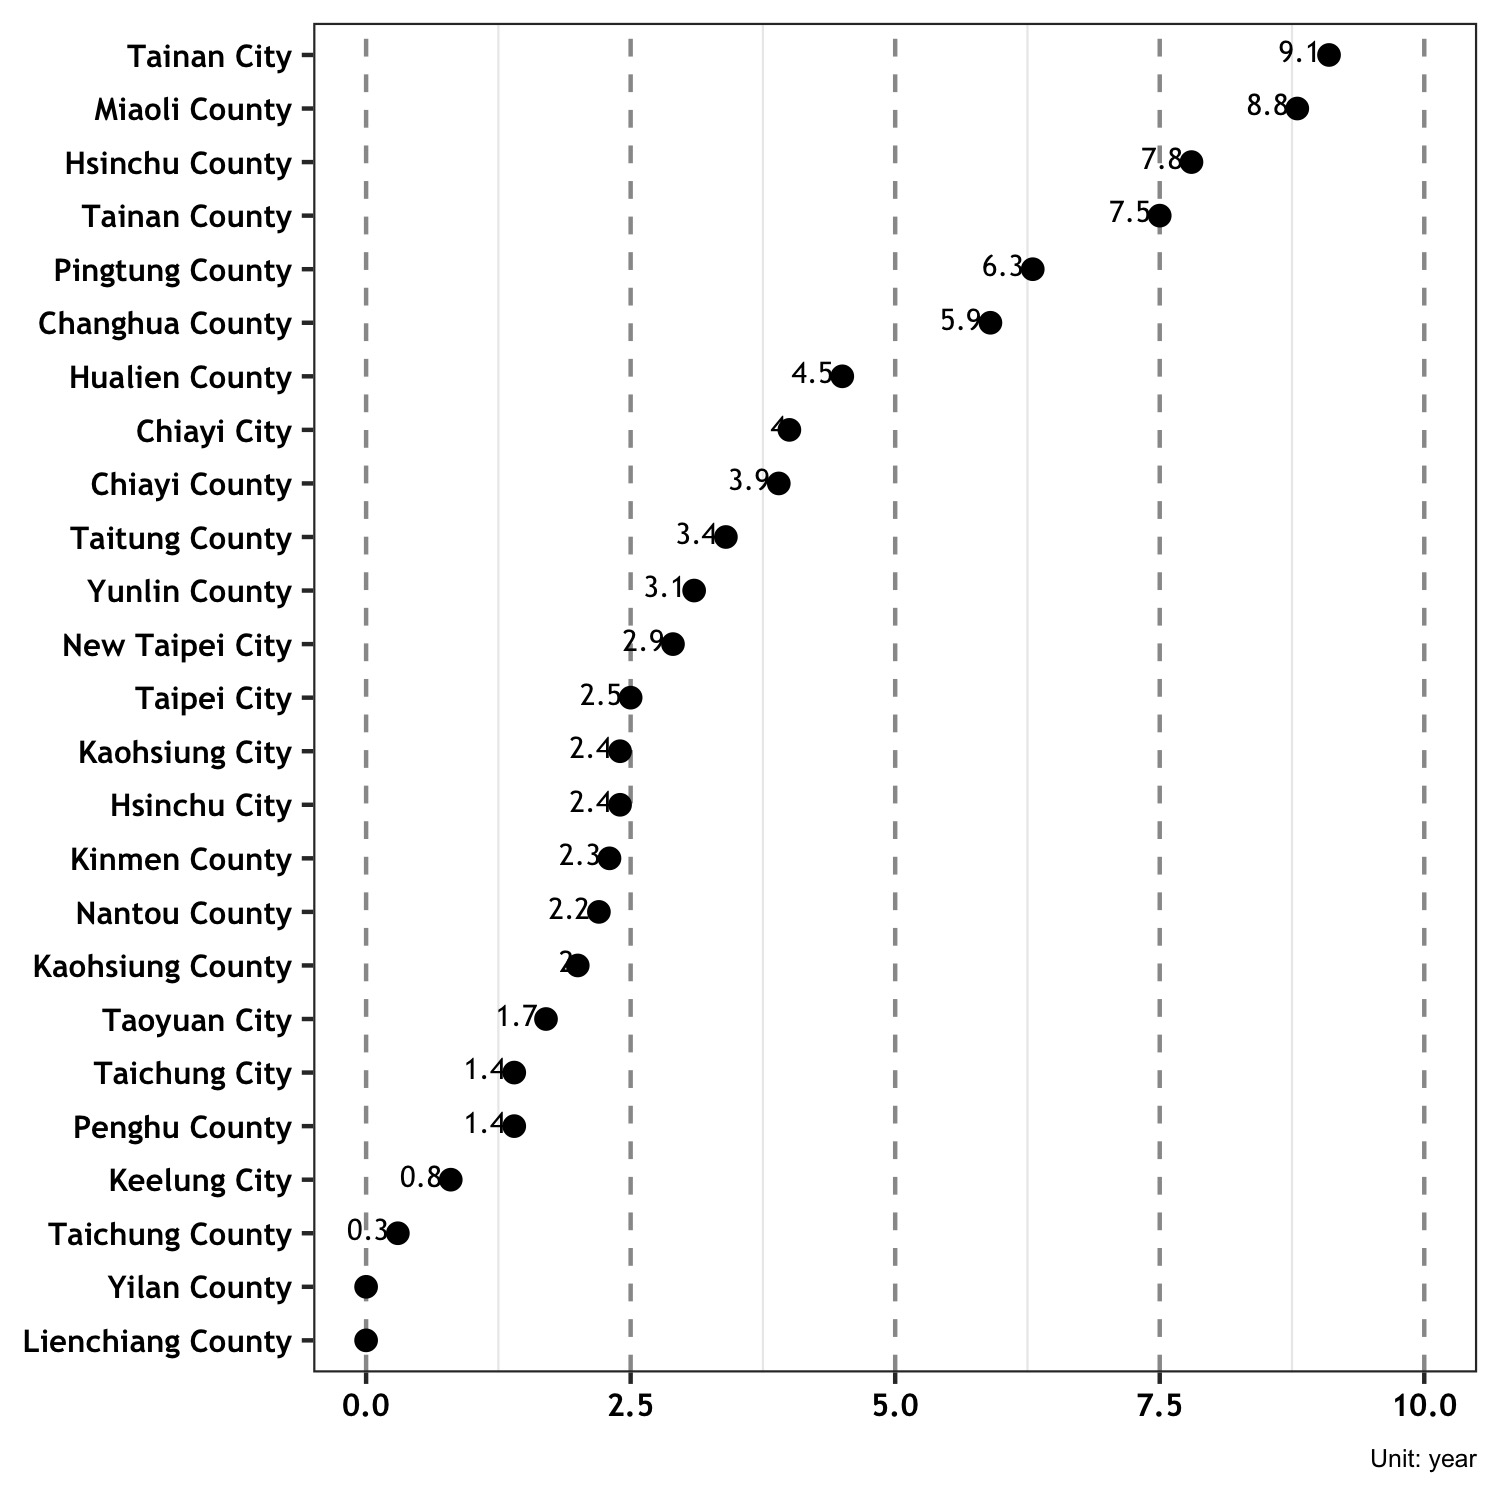
\includegraphics[width=7cm,height=7cm]{04-Chapter-Four/image/figure5-1.jpeg} & 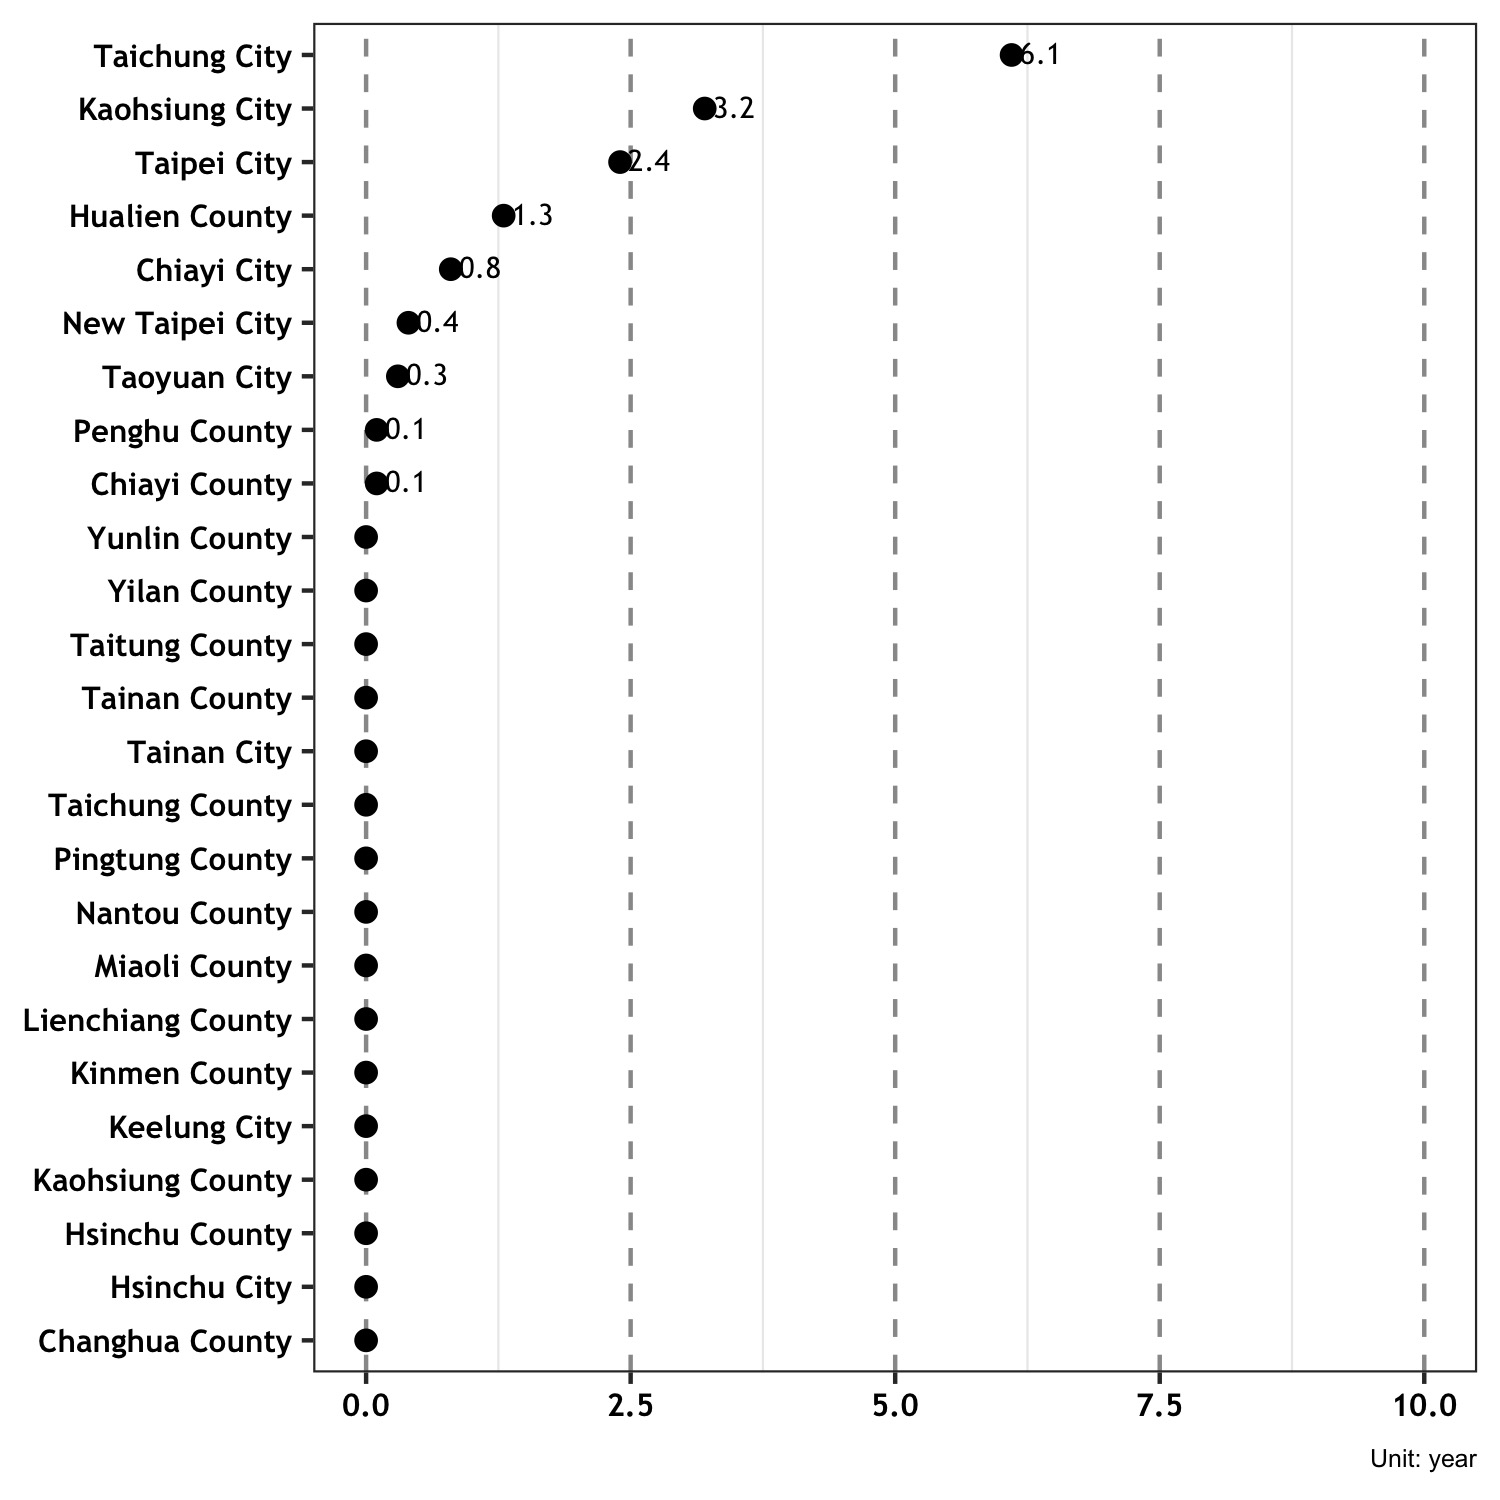
\includegraphics[width=7cm,height=7cm]{04-Chapter-Four/image/figure5-2.jpeg}\tabularnewline
\end{tabular}
Note: This figure depicts the decomposition of the mayor's experience in a pooled mean year.
\end{figure}


\subsection*{Standing Committee Members}


\begin{table}[!htbp]
\caption{The Estimation for the Mayor with Years of Experience \\ 
        as Legislators and Ministers \label{tab:table3}}
\centering{}{\small{}}%
\scalebox{0.85}{
\begin{threeparttable}

\begin{tabular}{lcccc}
\toprule 
\multicolumn{5}{l}{Dependent Variable:}                                                                \\
\multicolumn{5}{l}{\textbf{log (Revenue Support Grant)}}                                               \\
\midrule
                                &  Model (1)      & Model (2)       & Model (3)  & Model (4)          \\
\midrule
$\Delta{\textbf{\textit{ministers}}}$   & 0.267           & 0.514         & 0.682         & 0.046            \\
                                 & 0.364           & 0.406         & 0.418         & 0.348            \\
$\Delta{\textbf{\textit{legislators}}}$ & 0.397$^{***}$   & 0.283         & 0.286         & 0.285$^{*}$      \\
                                 & 0.167           & 0.185         & 0.189         & 0.162            \\
\textbf{standing committee   }                & 0.051           & 0.136$^{***}$ & 0.138$^{**}$  & 0.043            \\
                                 & (0.051)         & (0.059)       & (0.060)       &(0.049)           \\
\textbf{seniority }                          & 0.011           & 0.051         & 0.057         & 0.103            \\
                                 & (0.217)         & (0.177)       & (0.179)       &(0.214)           \\
\textbf{power committee}                  & 0.655$^{***}$   & 0.142         & 0.111         & 0.517$^{***}$.   \\
                                 &(0.117)          & (0.103)       & (0.104)       &(0.121)           \\
\textbf{committee chair}                   & 0.117           & 0.045         & 0.038         & 0.212.           \\
                                 &(0.188)          &(0.150)        & (0.151)       &(0.181)           \\
\textbf{mayoral election}                & 0.017           & 0.018         & 0.020         & 0.385$^{***}$    \\
                                 &(0.055)          &(0.043)        & (0.044)       &(0.104)           \\
\textbf{co-partisan mayors}                & 0.040           & 0.040         & 0.044         & 0.040            \\
                                 &(0.050)          &(0.041)        & (0.041)       &(0.049)           \\
\textbf{\% mayor vote}                      &0.856$^{***}$    & 0.719$^{***}$ & 0.716$^{***}$ & 0.7157$^{***}$   \\
                                 &(0.188)          & (0.1621)      & (0.163)       &(0.183)           \\
\textbf{\% pres. vote}                       & 0.359           & 0.176         & 0.149         & 0.006            \\
                                 & (0.231)         & (0.186)       & (0.188)       &(0.256)           \\
\textbf{co-partisan legislator}           &0.215$^{***}$    & 0.189$^{***}$ & 0.181$^{***}$ & 0.122            \\
                                 &(0.050)          &(0.041)        &(0.041)        &(0.135)           \\
\textbf{\% unemployed}                    & 7.564$^{***}$   & 5.033$^{***}$ & 4.994$^{***}$ &12.940            \\
                                 & (3.518)         & (2.846)       & (2.863)       &(8.312)           \\
\textbf{special cities}                   & 0.692$^{***}$   & 0.102         & 0.078         & 0.703$^{***}$    \\
                                 & (0.067)         & (0.117)       & (0.130)       &(0.064)           \\
\textbf{Constant}                         & 1.938$^{***}$   & 2.053$^{***}$ &               &                  \\
                                 & 0.2067          & 0.197         &               &                  \\
\midrule 
\textbf{No. of observations}             &367              & 367           & 367           & 367              \\
\textbf{adjusted \textit{R}$^{2}$}                   & 0.461           & 0.197         & 0.155         & 0.449            \\
\textbf{model types}                       & Pooled OLS      & RE            & FE            & FE               \\
\textbf{municipality fixed effects }       &                 &               & $\checkmark$  &                  \\
\textbf{fixed effects by year}               &                 &               &               & $\checkmark$     \\
\midrule

\end{tabular}
     \begin{tablenotes}
     Note: * \(p<0.10\),** \(p<0.05\), *** \(p<0.01\). \\ Robust standard errors in parentheses. Standard errors are clustered by municipality. Hausman test\ensuremath{\chi}2 (12)= 13.115 \ensuremath{p}-value = 0.3608 rejects the null hypothesis 
     \end{tablenotes}
     \end{threeparttable}
     }
\end{table}


Following the literature about the importance of legislative committee \citep[e.g.,][]{Martin2014,Wang2013,Hsiao2007, Matsuo2012}, I add another dummy variable as an explanatory variable, \textbf{Standing Committee} in \autoref{tab:table3}, indicating if the mayor has ever had committee membership in the Legislative Yuan. The regression model can be extended as


\begin{equation} \begin{split} \ensuremath{y_{i,t+1}^{grant}}= \ensuremath{\beta_{1}{\Delta minister}_{i,t} +\beta_{2}{\Delta legislator}_{i,t} + \\ \beta_{3}{Standing Committee}_{i,t} +\\ X_{i,t}\gamma + \alpha_{i} + \delta_{t} + \varepsilon_{i,t}}. \end{split} \end{equation} 

Then, I observe some shifts of coefficients in magnitude, especially $\Delta\textit{\textbf{legislators}}$. In column 3 with favoured Random Effect model, \textbf{standing committee} is both statistically and economically significant. This means that when I control for \textbf{standing committee}, a large proportion of significance transfers to this indicator, making it a vital variable in explaining changes in resources among municipalities. Unsurprisingly, the originally significant variable, $\Delta\textit{\textbf{ministers}}$, in \autoref{tab:table3}, is reduced to insignificance.

\begin{figure}[!htbp]
\begin{singlespace}
\begin{centering}
\caption{The Effect of Standing Committee on the Marginal Increase in \\ Revenue Support Grant \label{fig:figure6}}
\par\end{centering}
\end{singlespace}
\begin{centering}
\begin{tabular}{c}
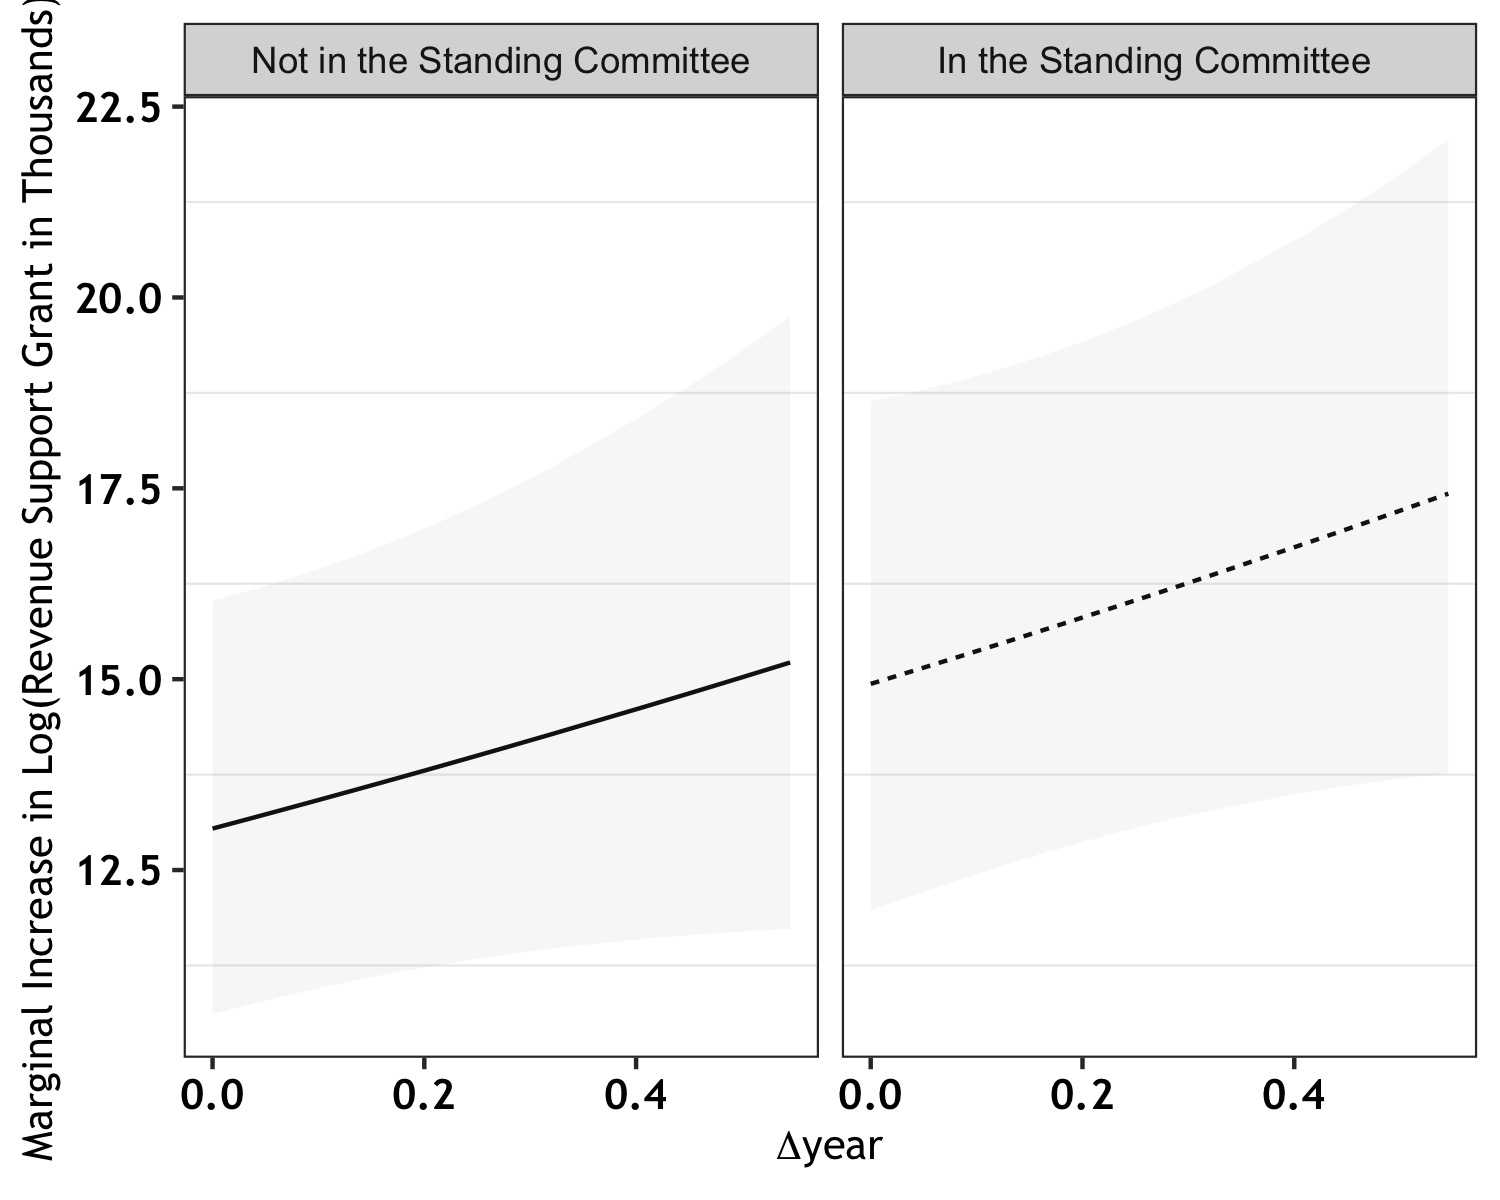
\includegraphics[width=12cm,height=7.5cm]{04-Chapter-Four/image/figure6.jpeg}\tabularnewline
\end{tabular}
\par\end{centering}
Note: The figure present regression coefficients adjusted by all control variables at 95\% percent confidence intervals.
\end{figure}
\textcolor{black}{{} }


This finding suggests that, in explaining the distribution of resources, the effect of $\Delta\ensuremath{legislators}$ is more significant than that of mayors' experience as ministers. More interestingly, the significance of membership in a standing committee even outplays that of the experience as legislators in general, suggesting that the distribution of resources is indeed biased, in favour of municipalities whose mayors served as legislators and among all those mayors with legislator background, prior experience as a standing committee member seems to grant municipalities more privilege in obtaining inter-governmental transferred resources.\footnote{In light of the Hausman test in favour of RE model, I use the estimates from Model (3) in \autoref{tab:table3}.} 

\section*{\centering Conclusion}

Since the emergence of a direct legislative election system in 1992 and a direct presidential election in 1996, central government spending has become inherently susceptible to manipulation for electoral purposes as an inevitable side-effect of such systems. 

The literature on distributive politics has covered various research topics that explain the variation in the distribution of government resources in different contexts and countries. By investigating whether mayors exploit the privilege of being more network-like to the government party to obtain more grants, I identify potential impacts between each mayor's prior years of experience in the central government and the number of financial resources that local government receives. The findings are generally consistent with the literature \citep{Keefer2008,Keefer2009} that a mayor with more connections to the central government obtains substantially more distributive benefits than a political neophyte with less or no political experience.

Finally, while the inequitable distribution of resources is prevalent in most new democracies, our findings are a tentative discovery of the importance of local governments' leaders. I find that municipalities with more years of experience as legislators are allocated more political resources from the central government. The impact is more substantial when mayors have more experience in standing committees.
%%%%%%%%%%%%%%%%%%%%%%%%%%%%%%%%%%%%%%%%%%%%%%%%%%%%%%%%%%%%%%
%%                This is Chapter 5 (Conclusion)            %% 
%%%%%%%%%%%%%%%%%%%%%%%%%%%%%%%%%%%%%%%%%%%%%%%%%%%%%%%%%%%%%%
\chapter{Conclusion}
\clearpage
This thesis examines the political behavioural change of local legislators in their legislative voting and parliamentary questions asked to the executive government (The Executive Yuan) after an electoral reform. Specifically, the causal impact of the 2008 reform of the Taiwan electoral system is carefully examined, combined with various newly developed and innovative approaches. The findings of the thesis contribute to the large body of literature on the origins and consequences of electoral systems.

The most direct consequence of Taiwan's electoral reforms is that it exemplified the impact of electoral changes on party relations and individual legislative behaviours. To put it differently, SNTV made it easy for extremists to be elected without winning a large share of votes  \citep[e.g.,][]{Cox1987, Cox1990, Cox1996, Cox2008, Carey1995}. In particular, SNTV allowed the district magnitude to exceed one and led to a dispersed distribution of within-party ideology spectrum \citep[e.g.,][]{Stockton2010, Carey1995, Catalinac2019, Catalinac2017, Catalinac2016}, as well as an increased number of candidates who run on personal reputation and regional organisations. 

Aware of the side effects of SNTV, mainstream parties jointly initiated an election reform, aiming to reduce co-partisan conflicts and improve the political atmosphere in congress. The focus of this reform was expected to improve partisan conflicts within congress by contracting the number of legislators to be elected. In addition, the literature anticipates that under this system, electoral competition is winnowed down to two parties \citep[e.g.,][]{Catalinac2017, Downs1957, Duverger1954, Merrill2002, Magar1998, Reed2001}. Therefore, SMD was chosen as the desirable electoral system in lieu of the SNTV \citep[e.g.,][]{Yu2008, Liao2013, Jou2009}.

In general, this thesis investigates how legislators position themselves in response to an electoral system from the single non-transferable vote to single-member districts. Three main chapters that analyse historic legislative archives are developed extensively to demonstrate the impact of the reform on legislators' representation and preference, using several new and rapidly evolving estimation methods. To narrow down, the thesis focuses on the following three research subjects: Does electoral reform mitigate intraparty competition and political polarisation between parties? Does the reform decrease legislator's intention to particularistic policies? In what follows, I describe the structure and briefly summarise the findings and contributions of the thesis.

In the \autoref{chap:ch2} , I utilise the ideal point estimation to study the impact on legislators' preferences in relation to their party. The empirical evidence shows that intraparty fractionalisation increases while ideological differences between major parties are drastically polarised in the SMD. Controlling for yearly effects during the presence of the reform, however, I find that the impact of party division decreases as time goes by. In \autoref{chap:ch3}, I investigate how the reform changes legislator behaviour and tendencies toward constituencies. I investigate this topic using written parliamentary questions through an electoral reform from multi-member districts (MMD) to single-member districts (SMD). I find that legislators under SNTV are more likely to express political intention about pork barrel projects in written parliamentary questions. However, the institutional change subsequently demonstrates heterogeneous effects on mainstream parties and small parties, respectively.  

Last, I analyse intergovernmental transfers allocated to each municipality to explore how pork barrel spending is politically motivated by experienced mayors who used to serve as legislators in the Taiwanese Congress. In \autoref{chap:ch4} , I find that municipalities whose mayors had a longer career spent in the legislature are more likely to receive higher fiscal expenditures. The effect is even more substantial if the mayors have worked in legislative standing committees. On the contrary, mayors' prior political career in ministries does not significantly help their municipalities obtain the grant. The findings suggest that compared to experience as a central government official, their legislative career significantly impacts the distribution of the transfers to municipalities.

Overall, the reform may not immediately reduce intraparty conflicts but shortly exacerbate the inter-party relation when the new system is introduced. In addition, legislators' incentives for mainstream parties to run on personal votes significantly decreased, while the attention to general interest policies momentarily increased after the reform.

\section*{\centering Challenges and Limitations}

The thesis comes with several limitations. In \autoref{chap:ch2}, I demonstrate how the reform impacts legislators' ideological preferences and inter- and intra- party distance. However, since different topics were discussed in each session of roll call, the biggest challenge is to control for the session effect; i.e. there are heterogeneous effects across sessions that potentially affect the legislators' positioning. Specific topics related to political turmoils due to unforeseen incidents (e.g., Taiwan Strait Crisis in 1996, Million Voices against Corruption President Chen Must Go in 2006 and 2014 Sunflower Student Movement, 2019–20 Anti-Extradition Law Amendment Bill Movement in Hong Kong) and unexpected natural disasters (e.g., Typhoon Morakot, 1999 Jiji Earthquake, 2011 Fukushima Nuclear Disaster and Earthquake) are more likely to be discussed in current sessions. Therefore, these political incidents tend to polarise the main parties and disunite the distance between legislators and their parties. 

The best solution to tackle this issue would be to control for specific topics\footnote{i.e., the issues regarding the cross-strait and independence–unification.} in each session by manually including those incidents as much as possible as dummies in the econometric regressions. However, identifying and differentiating these contents one by one is exceptionally challenging. To this end, I address the problem concerning the heterogeneous sessional effects by including year dummies that can approximate the sessional effects. In \autoref{chap:ch3}, the effect of electoral reform is statistically significant in the specification of ideological dispersion between and between parties, suggesting that electoral reform increases the dispersion between parties between KMT and DPP, even after year dummies and demographic attributes are directly controlled in regression.

Second, the number of questions over years analysed in \autoref{chap:ch3} steadily decreases from 2003. This is due to the fact that the reduced amount of questions is potentially correlated with changes in media users and the occurrence of social media. In recent years, social media, such as Facebook and Twitter, has become a major platform for legislators to communicate with their voters. Therefore, legislators may utilise other means to view their points in relation to constituent concerns, such as Facebook.

Another limitation arises from the language transformation and its variation over time. As noted in \autoref{chap:ch3}, the training data of the pork barrel legislation were annotated by Dr Ching Jyuhn Luor \citep{Luor2008, Luor2009} between 2007 and 2009. That is to say, the deep learning architecture is only trained by learning to identify the pork barrelling features in the legislation in a given limited period, which potentially fails to comprehensively discover implicit notions invented after 2009. With BERT's self-attention mechanisms, the BERT-based framework may assist the machine classifier by simulating a similar skill set to the human brain that can identify more complex or unseen concepts derived from the labelled data to understand the underlying pork barrel features.

% With insightful literature  on the origins and consequences of electoral systems (e.g. Huang 2017; Göbel 2012; Carey and Shugart 1995; Hsu and Chen 2004; André, Depauw, and Shugart 2014; André, Freire, and Papp 2014), the thesis attempts to estimate the  changes of each legislator on their legislative voting and parliamentary questions asked to the executive government (The Executive Yuan). 
% The numerous studies have described that voters' ideological positioning along the left-right ideological spectrum in Taiwan is largely determined by the stances of each major parties (KMT and DPP) that takes on the issue of cross-strait relations \citep[e.g.,][]{Clark2012, Fell2004, Huang2017}. 
% Disrupted Careers leading to a subnational shift in particularism by ex Congressional mayors retaining connection to national politics


\section*{\centering Possibilities for Future Research}
First of all, understanding the positions of parties and legislators is fundamental to conceptualising party cohesion and their representation in most democracies. With parliamentary questions and topics classified by the official website,\footnote{The website of the Legislative Yuan} I can use the data set to estimate intraparty heterogeneity and variability in issue attention by looking at what and why legislators are more likely to oversee ministry officials on one specific topic than others. I can estimate the position of each legislator on the left-right dimensions using the keywords extracted from the questions that legislators request for information on policies and activities of ministerial officials. This is important to see how the electoral reform shapes legislators' issue attention and varies across time and the different electoral systems. The findings may shed new light on providing a different approach to measuring party cohesion and understanding changes in political behaviour in representation and political accountability through electoral reform.

Second, the work by \citet{Catalinac2016} has looked at the relationship between electoral reform and the behaviour of legislators covering pre- and post-reform periods by analysing the election manifesto using the Latent Dirichlet Allocation topic model. The paper successfully identified that the Liberal Democratic Party (LDP) candidates in the SMDs expressed more programmatic policies, such as national policies, and promised fewer pork barrel goods to the district. Likewise, I can apply a similar approach to clustering by discovering the variation of words frequently used when Taiwan's reform occurred. This method offers the advantage of combing through massive amounts of text in extensive document collections without going through the content in advance. 

However, topics extracted by the LDA method is generally not guaranteed to be well readable, especially in an unspaced language like Mandarin.\footnote{LDA substantially identifies each document as the mixture of topics by describing a distribution of words but assuming each word's equal importance. Mandarin is one of the unspaced languages, meaning it is written without spaces between characters and words.} Therefore, the performance of topic terms in each classification group may not provide explicit information if all part-of-speech (POS) tags are included. Particularly when handling the context of Taiwan politics, we need extra caution when text preprocessing, as there are some special terms, such as names of politicians and political institutions, as well as collocations.\footnote{In the thesis, I will train my language model (parser) based on an existing model to improve performance and classification prediction in Chinese.} To resolve this, I will manually augment the current pre-trained language model (UDPipe Traditional Chinese GSD 2.8 created by \cite{Straka2016, Straka2017}) for the POS task by enriching the training text data following the structure of the CONLL-U format. Once having these tags and linguistic features, I can extract a set of keywords and remove irrelevant the POS tagset such as auxiliary tokens, punctuation and irrelevant interjections and conjunctions.

In addition, previous works by \citet{Yu2013, Martin2015, Lau2014} suggest the coherence score (used to measure the quality of the topic model) can be improved by adjusting the elements of part of speech tags \textemdash limiting the corpus to nouns. Considering the unspaced feature in Mandarin, the future project will follow a similar approach to generate the LDA topic model by keeping specific POS tags in Chinese (such as nouns, verbs and adjectives), which is more efficient for summarising the multitude of topics and improving semantic coherence.\footnote{This approach can be utilised to extract more informative linguistic features and noun phrases in Chinese.}

In the third place, I anticipate combining estimates from legislative roll calls and parliamentary debates. Therefore, I can parallelly calculate each legislator' the difference and variance between political positions derived from roll calls and words expressed in the debates on salient topics such as same-sex marriage and cross-strait issues across the legislative sessions. This intrigues me if I can explain why and how legislators present their preferences consistently in both voting and speeches while some do not. I would like to see some legislators' voting preference correlates with their speech ideal points whereas some of them do not. 

Last but not least, this thesis contributes some applicable codes and packages for reproducibility to the open-source community and academia. For textual data, I have written a Python program (\href{https://davidycliao.github.io/legisCrawler}{davidycliao.github.io/legisCrawler}) for scrapping parliamentary documents on the official website of the Legislative Yuan (Taiwanese Congress) and attempted to implant an additional module for getting a corpus of parliamentary debates. For this purpose, I also have developed an R package (\textit{LegisTaiwan} \href{https://davidycliao.github.io/legisCrawler}{davidycliao.github.io/LegisTaiwan}) that requests voting records of legislation via the official API of the Taiwan Legislative Yuan Library. Further, \autoref{chap:ch3} looks at the proportion of parliamentary questions devoted to particularistic goods. To measure these quantities, I have trained a dynamic convolutional neural networks on top of the BERT model to identify pork-barrel features. The source code is written in Python using TensorFlow 2.4 and made available on the repository (\href{https://github.com/davidycliao/PorkCNN}{github.com/davidycliao/PorkCNN}). The application of this repository can be extended to other classification tasks (i.e., hate speech and extremism on the Internet). Also, it can be used for similar research (i.e. identifying the media post of the legislator on Facebook) that aims to quantify pork barrel characteristics in the context of Taiwan politics using Traditional Chinese. 

However, those codes and packages were created in 2019, 2020 and 2022, respectively. For codes written at different times, their functions and modules only target a specific type of data analysis to satisfy a certain purpose. Therefore, the original layout in the packages accumulates excessive expansion in each module, leading to issues of feature creep and making those programmes hard to maintain simultaneously. With recent advancements in the integration of Python and R, those packages are required to be rewritten and integrated into the same building block.

%%%%%%%%%%%%%%%%%%%%%%%%%%%%%%%%%%%%%%%%%%%%%%%%%%%%%%%%%%%%%%
%%                    Appendix Setting                      %% 
%%%%%%%%%%%%%%%%%%%%%%%%%%%%%%%%%%%%%%%%%%%%%%%%%%%%%%%%%%%%%%
\appendix
% Replace \bibliographystyle{plainnat} with \bibliographystyle{agsm} (I learned this here.)
\printbibliography

\clearpage
%%%%%%%%%%%%%%%%%%%%%%%%%%%%%%%%%%%%%%%%%%%%%%%%%%%%%%%%%%%%%%
%%                  Appendix for Chapter 2                  %% 
%%%%%%%%%%%%%%%%%%%%%%%%%%%%%%%%%%%%%%%%%%%%%%%%%%%%%%%%%%%%%%
\chapter{Supplementary Materials of Chapter 2}
\clearpage
\section{Plots of Estimated Legislators' Ideological Positions\label{sec:Plots full}}

This section plots estimated legislators' ideological positions. \autoref{fig:session-plot} plots for the ideological positions of two major parties at a frequency of session. From session 7-1 (the electoral reform in 2008), legislators from the two-major parties underwent a phase of drastic ideological diverging, as the distributions for both parties started moving to both pole (political polarisation).  \autoref{fig:term-plot} displays estimated legislators' ideological positions for all minor parties (DPP and KMT excluded) at a frequency of year. \autoref{fig:individual_point} plots individual legislator's ideal point from two major parties, grouped by year.

\begin{figure}[H]
\caption{Estimated Legislators' Positions for Two Major Parties across the Legislative Sessions \label{fig:session-plot} }
\centering{}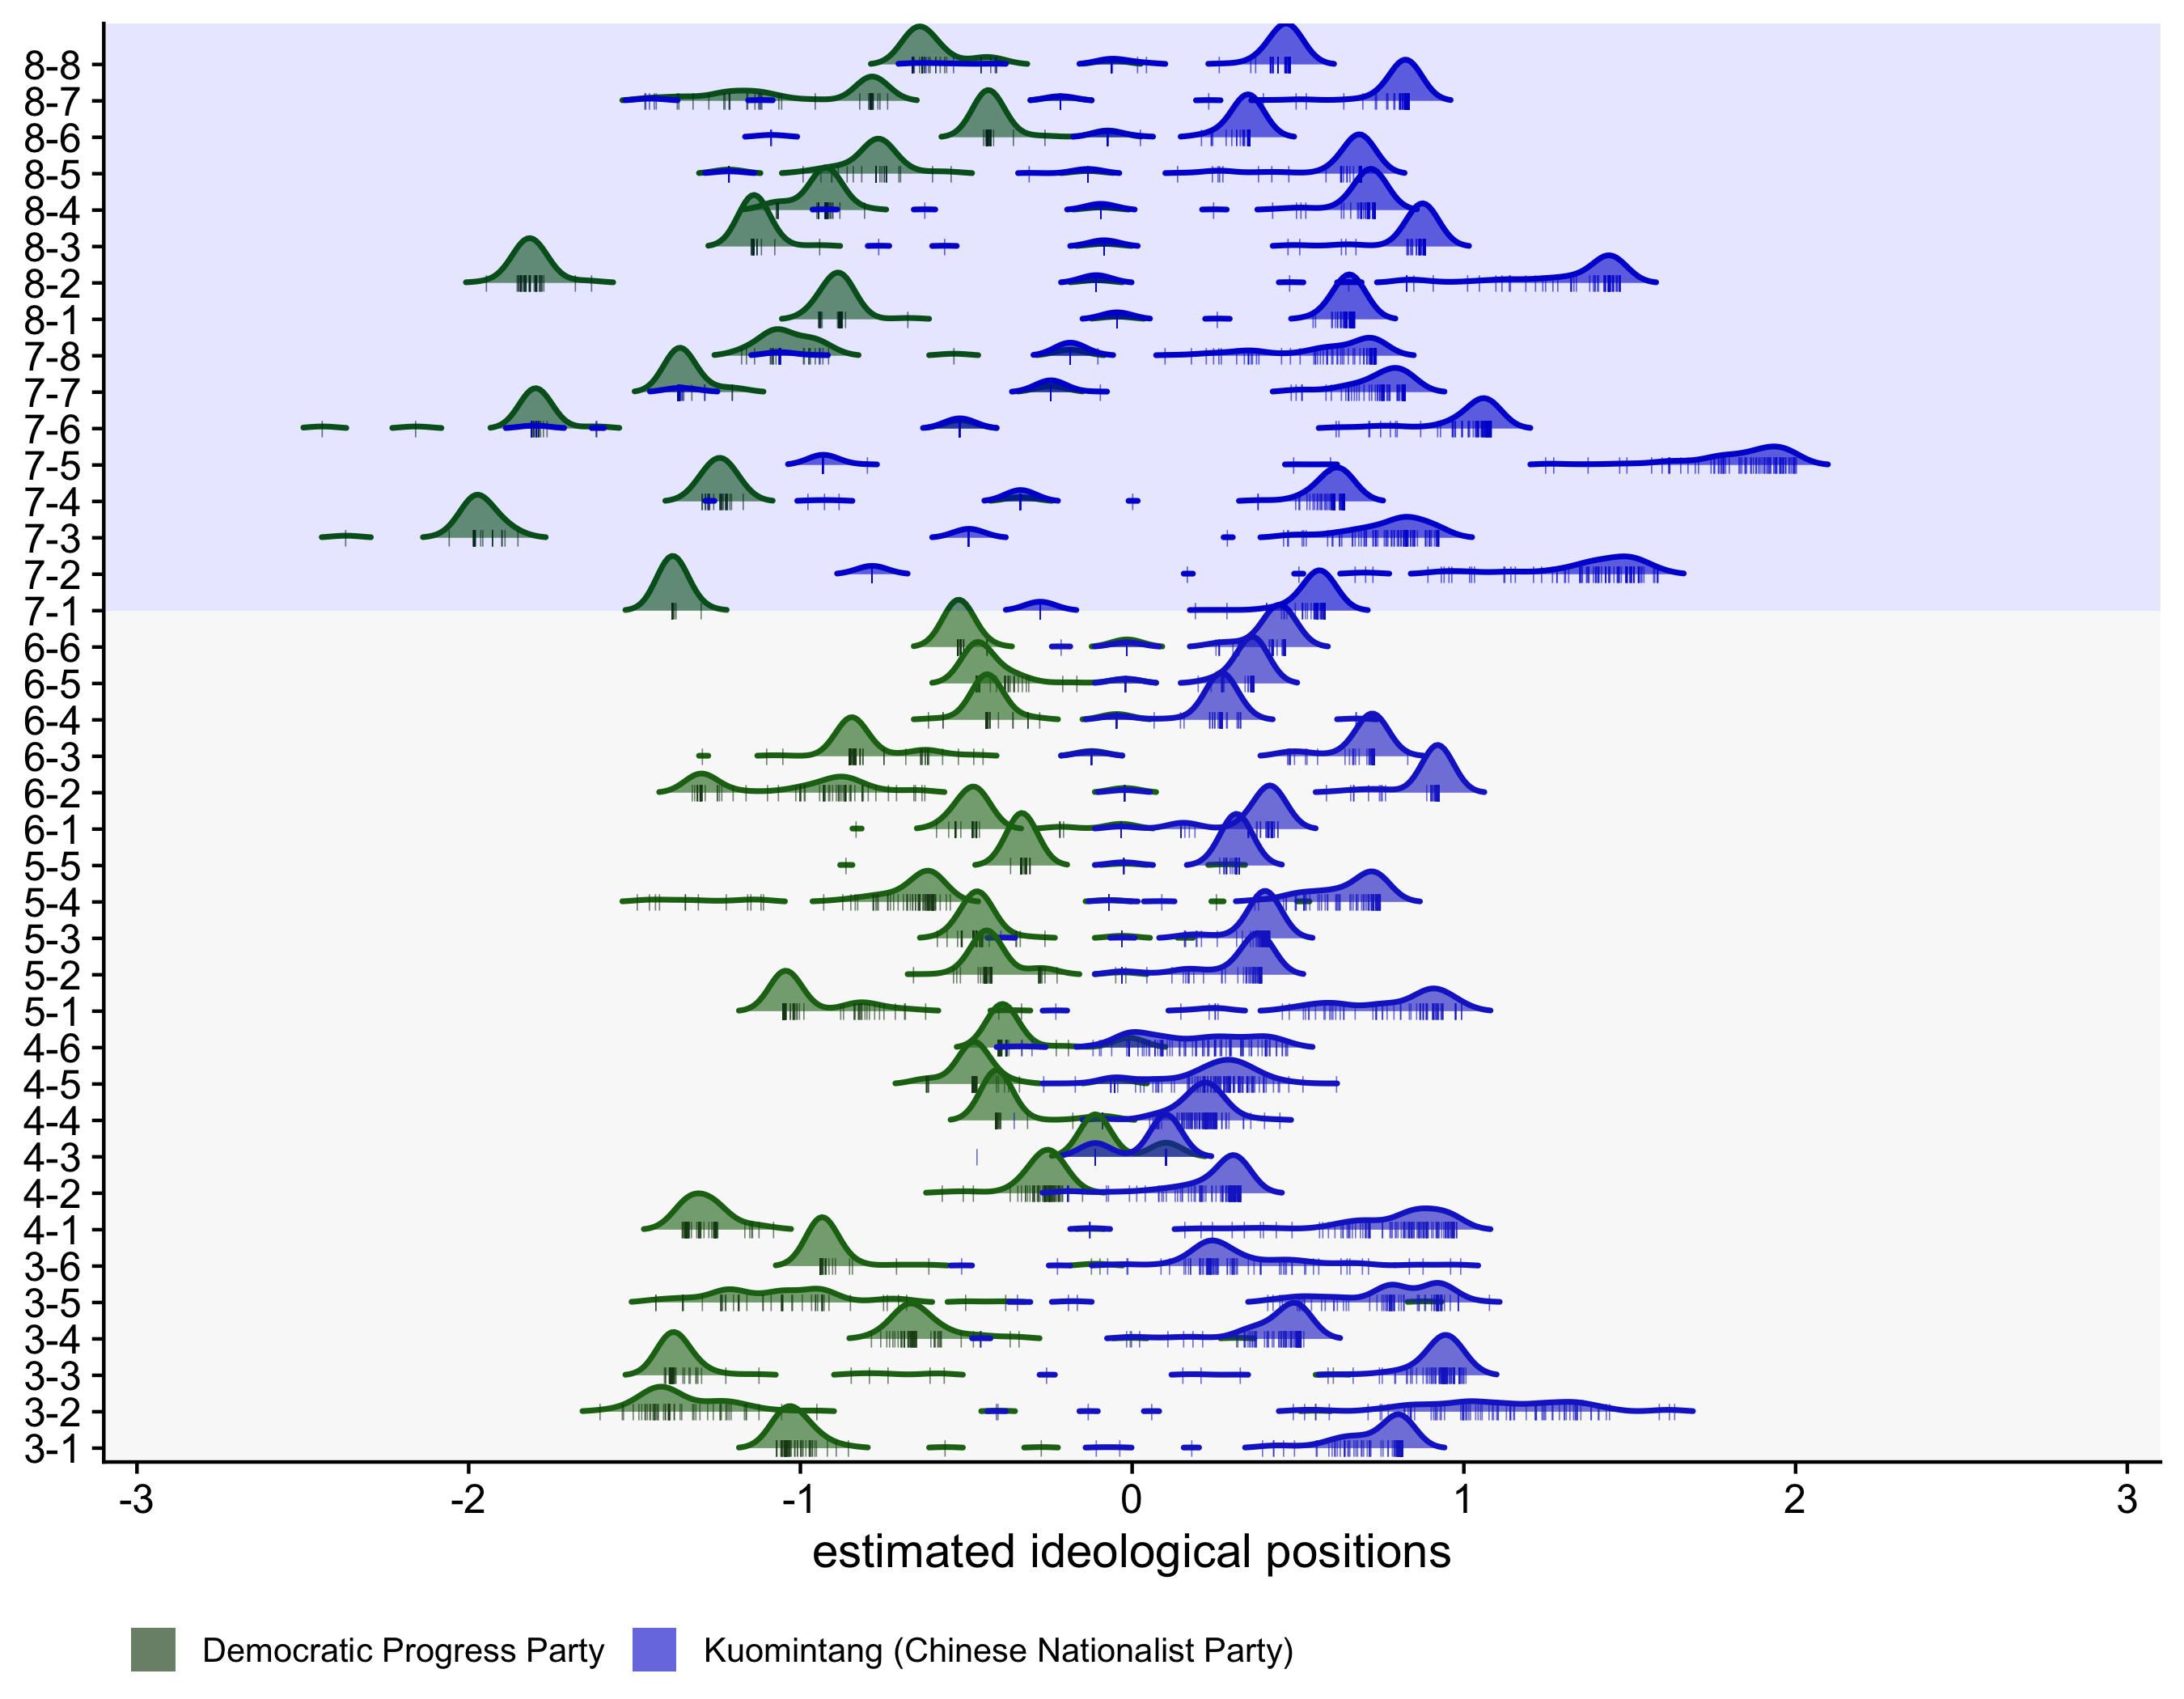
\includegraphics[scale=0.15]{02-Chapter-Two/image/major_postions_session}
\end{figure}

\begin{figure}[H]
\caption{Estimated Legislators' Ideological Positions for Small Parties across Years\label{fig:term-plot}}
\centering{}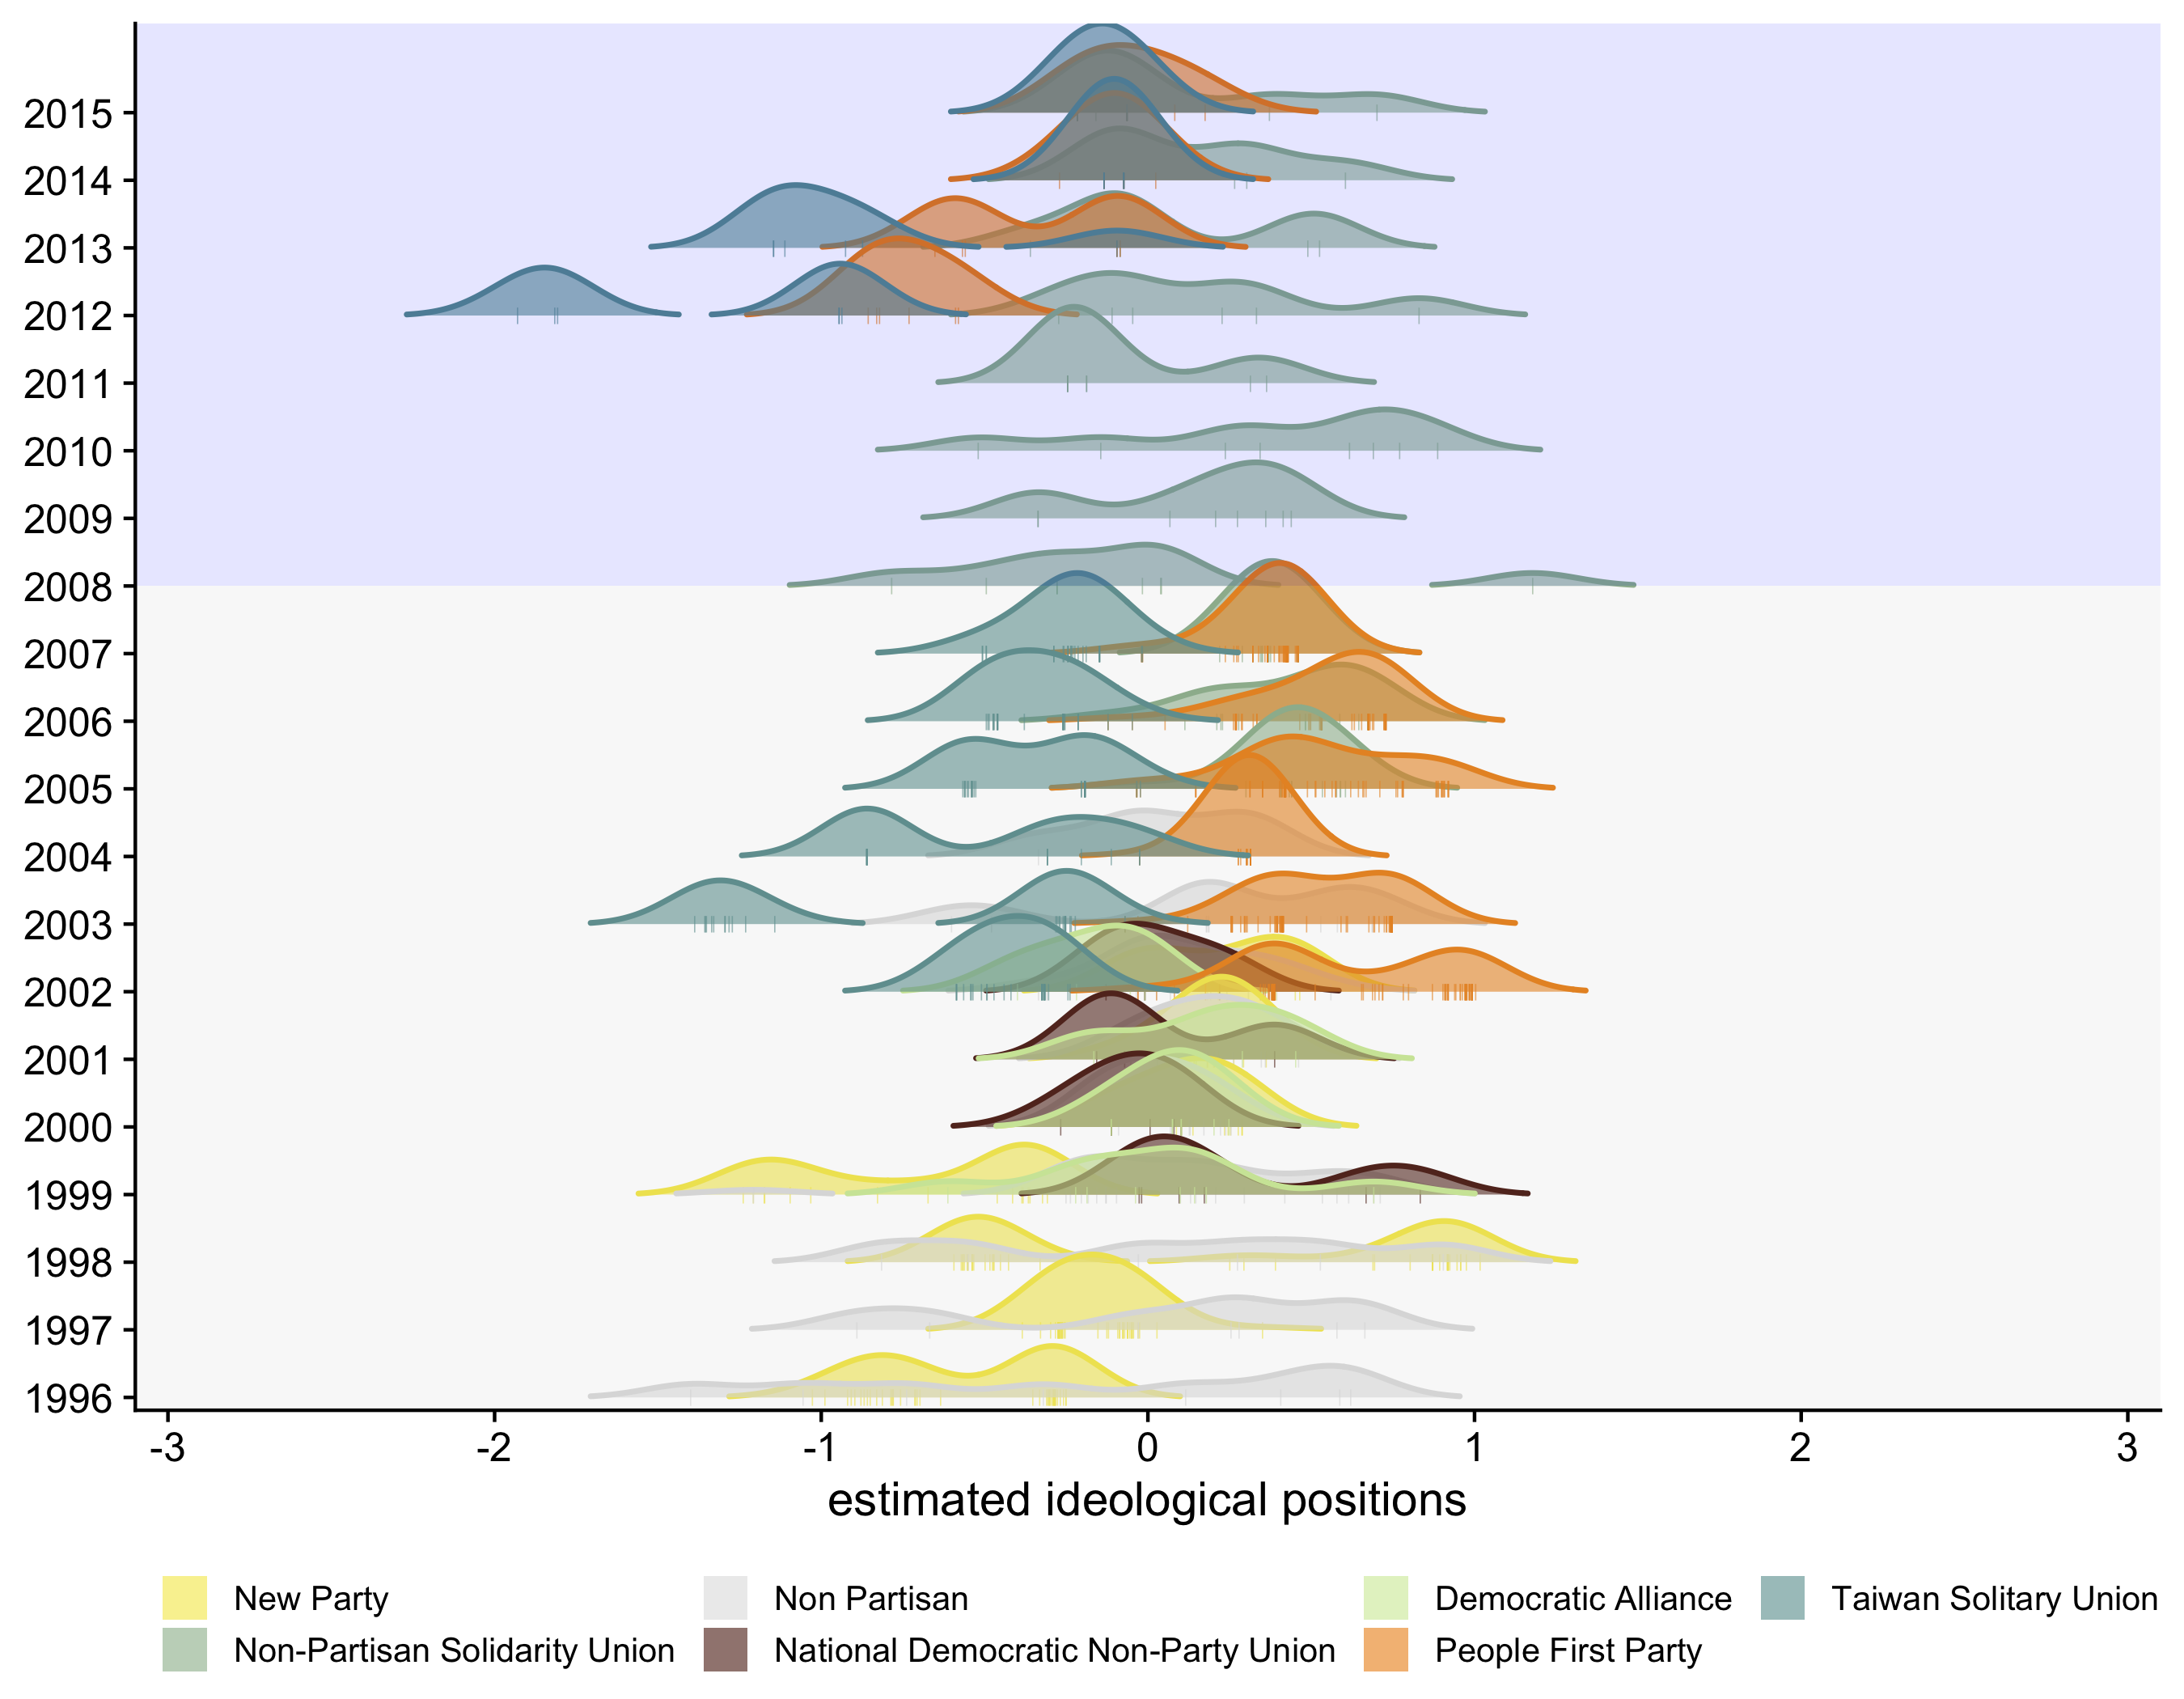
\includegraphics[scale=0.15]{02-Chapter-Two/image/minor_postions_year}
\end{figure}

\begin{figure}[H]
\caption{Individual Legislator' Ideal Point on a Single Dimension
for Two Major parties \label{fig:individual_point}}\centering{}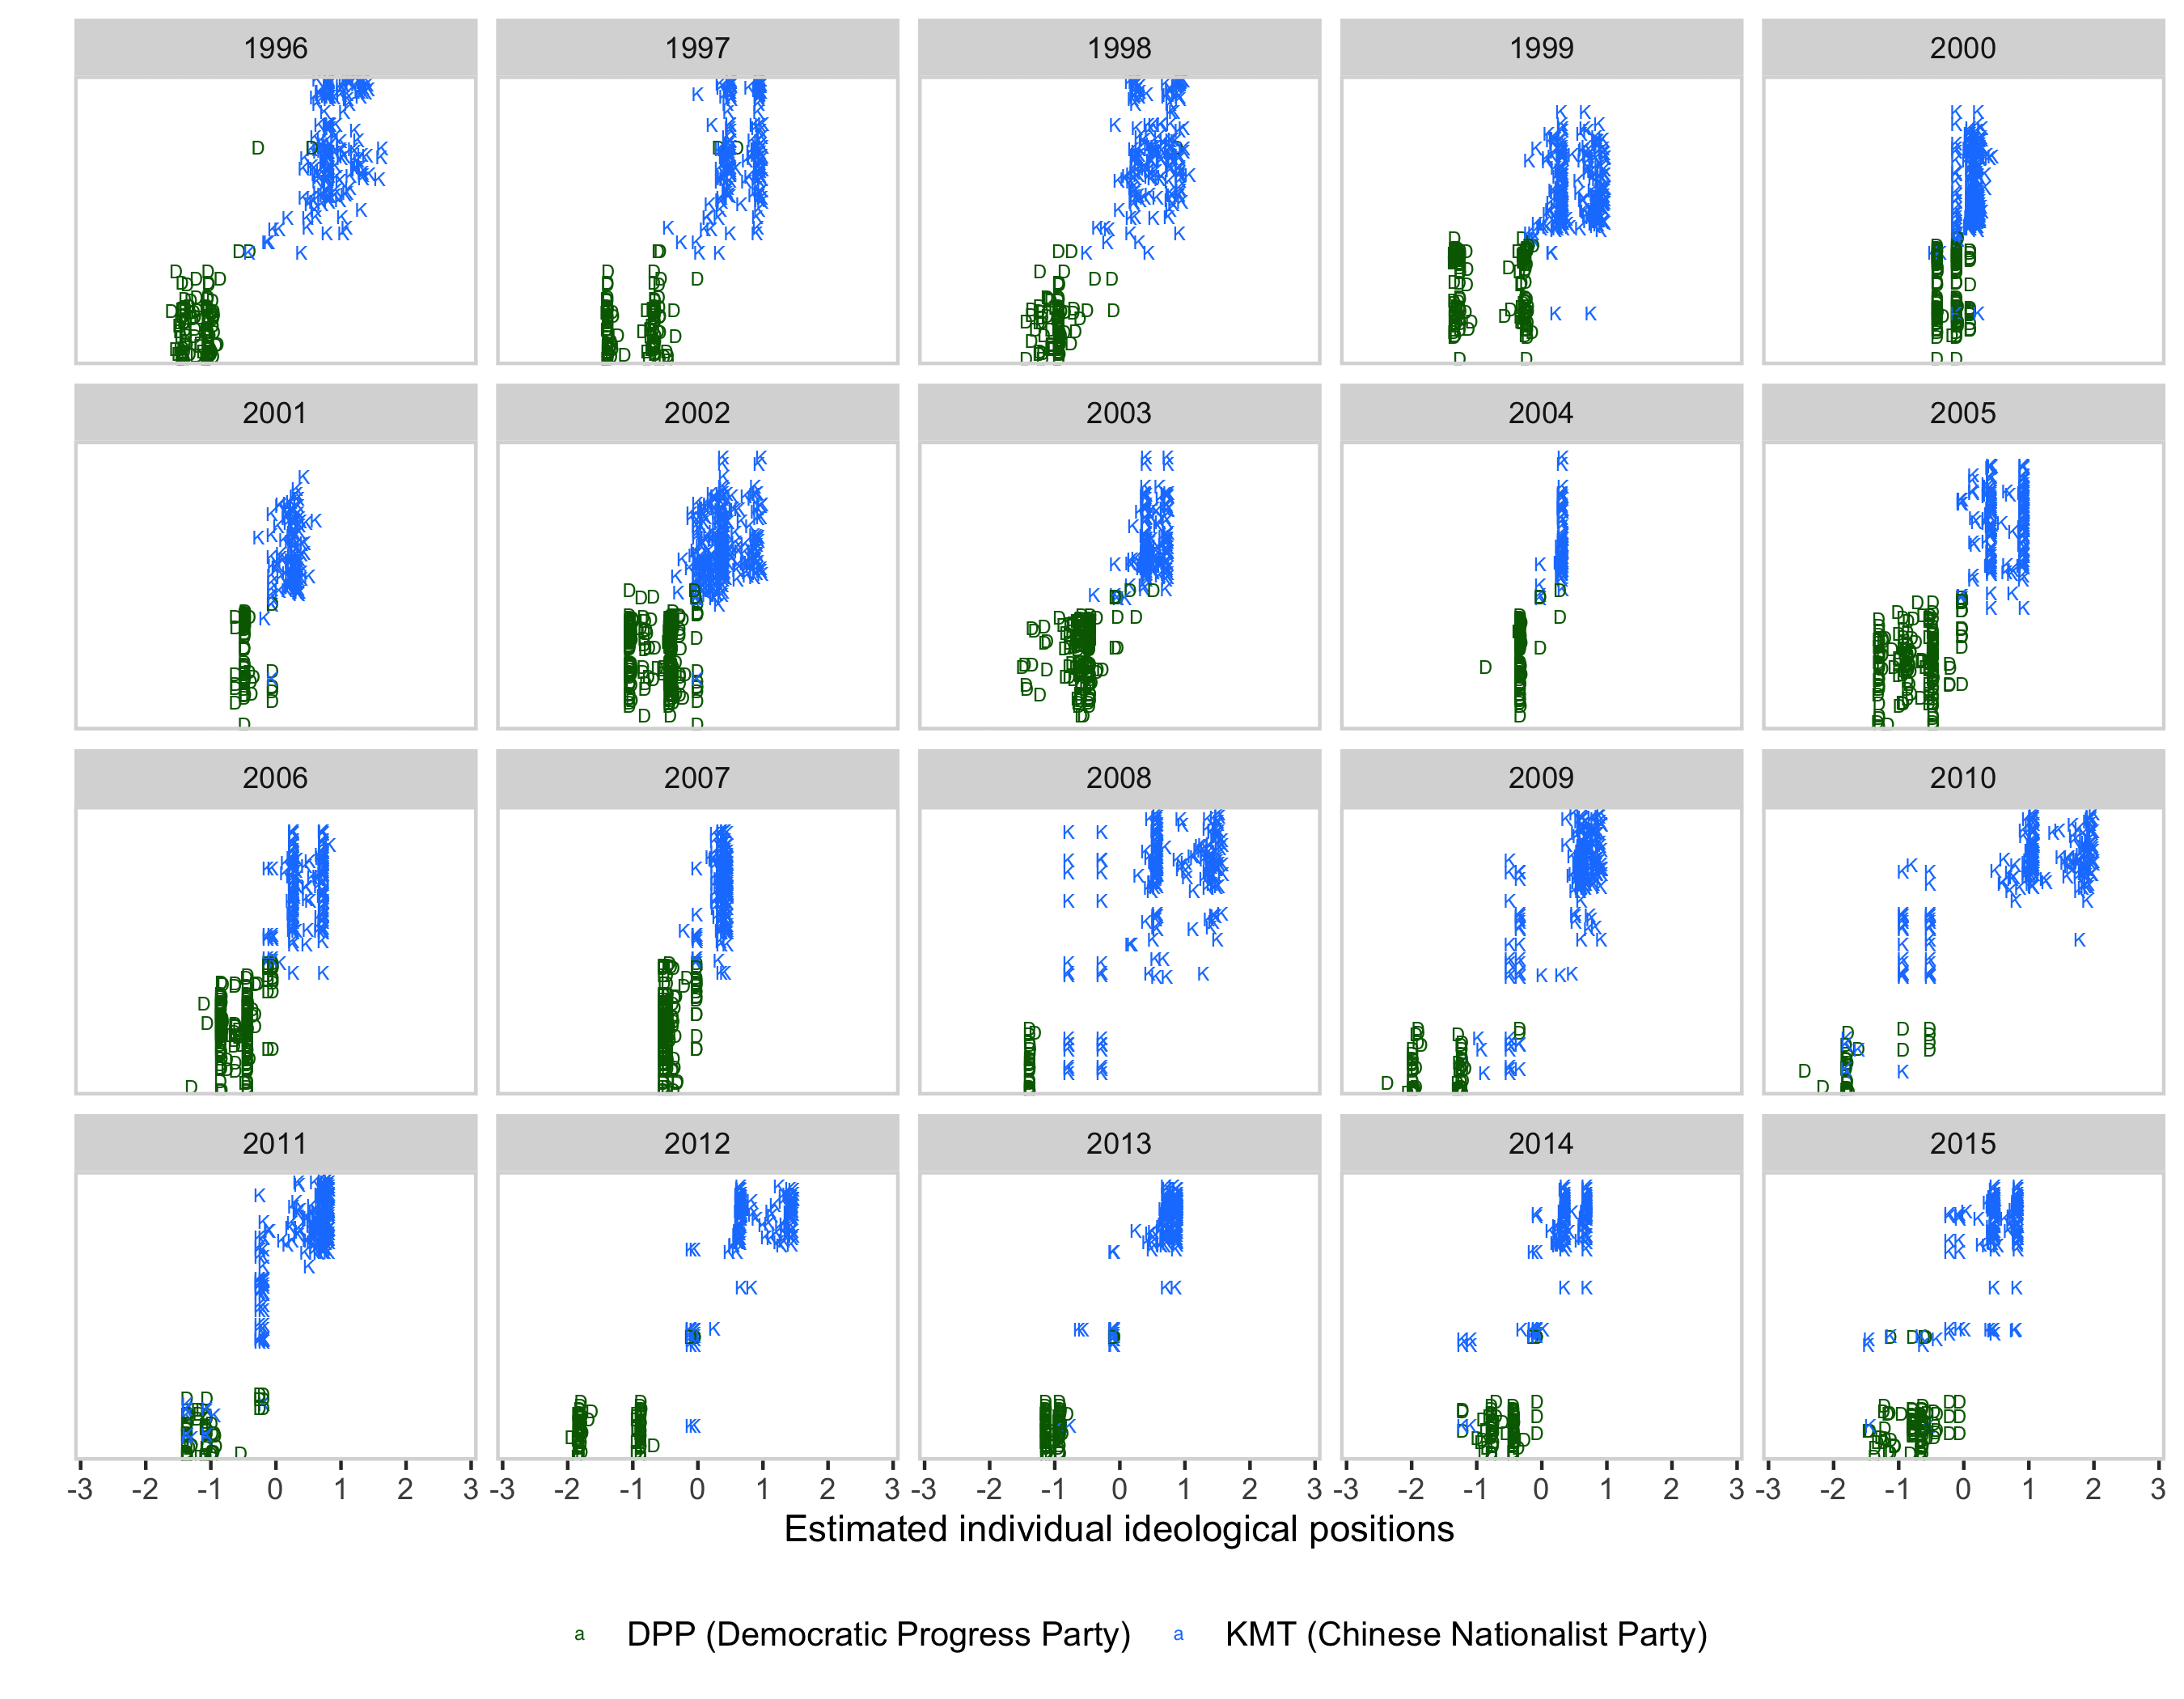
\includegraphics[scale=0.14]{02-Chapter-Two/image/individual_point}
\end{figure}

\clearpage

\section{\centering Robustness Estimation using Sub-samples\label{sec:robustness-check}}
\subsection{Inter-party Competition and Distances\label{subsec:robustness-inter-party}}

I replicate the estimations results from Section \ref{subsec:disunity-in-co-partisan} using data of DPP and KMT separately to ensure the result of between-party polarisation is not solely driven by any big parties. \autoref{tab:Inter_DM} reports the outcomes. Column 1 and 2 display the result using DPP and KMT respectively. The variable of \textbf{electoral reform } is statistically significant positive (at 1\% critical level in both columns), implying that the electoral reform significantly increases between-party ideological distance (political polarisation) regardless of the party-affiliation, consistent with the results found in \autoref{tab:intra-estimation}.


\begin{table}[H]
\caption{Legislator-level Interparty Distance\label{tab:Inter_DM}}
\centering{}%
\begin{tabular}{lcc}
    \toprule 
    \multicolumn{3}{l}{\textbf{Dependent variable:}}                          \tabularnewline
    \multicolumn{3}{l}{Interparty Legislator Ideological Distance}           \tabularnewline
    \midrule
                                & \textbf{DPP} & \textbf{KMT}                 \tabularnewline
    \midrule
electoral reform                & 23.000$^{***}$ & 13.132$^{***}$             \tabularnewline
                                & (2.916)        & (0.859)                    \tabularnewline
year                            & -0.205$^{***}$ & -0.263$^{***}$             \tabularnewline
                                & (0.015)        & (0.012)                    \tabularnewline
year $\times$ electoral reform  & -1.045$^{***}$ &  -0.460$^{***}$            \tabularnewline
                                & (0.153) & (0.047)                           \tabularnewline
marginal winning shares         & 0.017       & 0.250                         \tabularnewline
                                & (0.281)       & (0.136)                     \tabularnewline
intercept                       & 3.222$^{***}$ & 3.268$^{***}$               \tabularnewline
                                & (0.395)       & (0.316)                     \tabularnewline
legislator attributes           &     $\checkmark$    & $\checkmark$          \tabularnewline
district fixed effects          &     $\checkmark$    & $\checkmark$          \tabularnewline
    \midrule
No. of observations             & 1623          & 2547                        \tabularnewline
Adjusted R$^{2}$                & 0.28          & 0.27                        \tabularnewline
Prob > F                        & 0.00          & 0.00                        \tabularnewline
    \midrule
\multicolumn{3}{l}{{\footnotesize{}Robust standard errors are reported in parentheses. Asterisk}}   
                                                                              \tabularnewline
\multicolumn{3}{l}{{\footnotesize{}indicates significant level: {*}: p < 0.10; {*}{*}:p < 0.05; {*}{*}{*}:p < 0.01.}}                                                                                               \tabularnewline
\end{tabular}
\end{table}

\subsection{Disunited Distances between Co-partisan Legislators \label{subsec:disunity-robust}}

This section replicates the estimations results from Section \autoref{subsec:disunity-in-co-partisan} using observations of DPP and KMT separately to ensure the result of within-party disunity is not solely driven by any big parties. \autoref{tab:Intra_DM} reports the outcomes. Column 1 and 2 display the result using DPP and KMT respectively. The variable of \textbf{electoral reform} is statistically significant positive (at 5\% and 1\% critical level in column 1 and 2, respectively), implying that the electoral reform significantly increased within-party ideological distance regardless of the party-affiliation, consistent with the results found in  \ref{tab:intra-estimation}.

\begin{table}[H]
\caption{Legislator-level Intraparty Distance\label{tab:Intra_DM}}
\centering{}%
\begin{tabular}{lcc}
\toprule 
\multicolumn{3}{l}{\textbf{Dependent variable:}}                      \tabularnewline
\multicolumn{3}{l}{Intraparty Ideological Distance}     \tabularnewline
\midrule
                             & \textbf{DPP}  & \textbf{KMT}           \tabularnewline
\midrule
electoral reform             & 0.816$^{**}$  & 2.675$^{***}$          \tabularnewline
                             & (0.323)       & (0.411)                \tabularnewline
year                         & -0.007$^{**}$ & -0.005$^{**}$          \tabularnewline
                             & (0.003)       & (0.002)                \tabularnewline
year $\times$ electoral reform  & -0.037$^{**}$     & -0.123$^{***}$  \tabularnewline
                                & (0.017)           & (0.021)         \tabularnewline
marginal winning shares         & 0.046             & 0.018           \tabularnewline
                                & (0.069)           & (0.136)         \tabularnewline
intercept                       & 0.066             & -0.081          \tabularnewline
                                & (0.070)           & (0.124)         \tabularnewline
legislator attributes           & $\checkmark$      & $\checkmark$    \tabularnewline
district fixed effects          & $\checkmark$      & $\checkmark$    \tabularnewline
\midrule
No. of observations             & 1623              & 2547            \tabularnewline
Adjusted R$^{2}$                & 0.03              & 0.05            \tabularnewline
Prob > F                        & 0.01              & 0.00            \tabularnewline
\midrule

\multicolumn{3}{l}{\footnotesize{}Robust standard errors are reported in parentheses. Asterisk }           \tabularnewline
\multicolumn{3}{l}{\footnotesize{}indicates significant level: {*}: p < 0.10; {*}{*}: p < 0.05; {*}{*}{*}:}\tabularnewline
\multicolumn{3}{l}{\footnotesize{}p < 0.01.}                                                               \tabularnewline
\end{tabular}
\end{table}

\clearpage

\section{Addressing the Heterogeneity in Bills Voted across Year\label{sec:Addressing-the-heterogeneity}} 

Then, there is also the heterogeneity in years that could impact the legislature ideological position through voting decision, due to multiple reasons. First, in some years, bills voted were more likely to cause inter- or intraparty disagreement and thus, dispersion in ideological points. Second, in some years, the major social activities or events happened that also could cause disagreement or conflicts in the legislature. For example, in 2006, there was a mass campaign (\textit{Million Voices against Corruption}, President Chen Must Go) led by former DPP Chairman Shih Ming-teh (施明德) to pressure the President Chen Shui-bian (陳水扁) to resign. Therefore, I address the problem concerning the heterogeneity in year by controlling for as many years as possible.\footnote{Some years (2007, 2014 and 2015) are omitted due to multi-collinearity.}  \autoref{tab:heterogeneity of bills} reports the estimation results for inter-party analysis, with (column 2) or without controlling for other effects (column 1). As you can see, \textbf{electoral reform }is still statistically significant positive (at 1\% critical level) and are robust, meaning that the electoral reform caused higher level of inter-party dispersion between KMT and DPP, even if I introduce additional year dummies and control for the passage of time and other attributes.\footnote{Almost all year dummies are statistically significant at the 1\% critical level for both regressions, except year 2008. Estimated coefficients and standard errors for year dummies are omitted due to space limit.}  \autoref{tab:heterogeneity of bills} reports the estimation results for intraparty analysis, with (column 2) or without controlling for other effects (column 1). Similar results are obtained.

\begin{table}[ht]
\caption{Interparty Distance by Controlling for the Heterogeneity Effects from Different Years \label{tab:heterogeneity of bills}}
\centering{}%
\begin{tabular}{lcc}
\toprule 
\multicolumn{3}{l}{\textbf{Dependent variable:}}                                                            \tabularnewline
\multicolumn{3}{l}{Inter-party Ideological Distance}                                                        \tabularnewline
\midrule
                                & \footnotesize{\textbf{Interaction}} &                                      \tabularnewline
                                & \footnotesize{\textbf{+ Years}}     & \footnotesize{\textbf{(+ Controls)}} \tabularnewline
\midrule
\footnotesize{electoral reform} & \footnotesize{6.18$^{***}$}  & \footnotesize{6.401$^{***}$}  \tabularnewline
                                & \footnotesize{(0.818)}       & \footnotesize{(0.968)}        \tabularnewline
\footnotesize{year}             & \footnotesize{-0.361$^{***}$}& \footnotesize{-0.355$^{***}$} \tabularnewline
                                & \footnotesize{(0.010)}       & \footnotesize{(0.012)}        \tabularnewline
\footnotesize{year$\times$ electoral reform}   & \footnotesize{-0.147$^{***}$}   & \footnotesize{-0.158$^{***}$} \tabularnewline
                                & \footnotesize{(0.042)}       & \footnotesize{(0.050)}       \tabularnewline
\footnotesize{intercept}        & \footnotesize{5.050$^{***}$} & \footnotesize{5.598$^{***}$} \tabularnewline
                                & \footnotesize{(0.120)}       & \footnotesize{(0.246)}       \tabularnewline
\footnotesize{1997}             & $\checkmark$         & $\checkmark$  \tabularnewline
\footnotesize{1998}             & $\checkmark$         & $\checkmark$  \tabularnewline
\footnotesize{1999}             & $\checkmark$         & $\checkmark$  \tabularnewline
\footnotesize{2000}             & $\checkmark$         & $\checkmark$  \tabularnewline
\footnotesize{2001}             & $\checkmark$         & $\checkmark$  \tabularnewline
\footnotesize{2002}             & $\checkmark$         & $\checkmark$  \tabularnewline
\footnotesize{2003}             & $\checkmark$         & $\checkmark$  \tabularnewline
\footnotesize{2004}             & $\checkmark$         & $\checkmark$  \tabularnewline
\footnotesize{2005}             & $\checkmark$         & $\checkmark$  \tabularnewline
\footnotesize{2006}             & $\checkmark$         & $\checkmark$  \tabularnewline
\footnotesize{2005}             & $\checkmark$         & $\checkmark$  \tabularnewline
\footnotesize{2009}             & $\checkmark$         & $\checkmark$  \tabularnewline
\footnotesize{2010}             & $\checkmark$         & $\checkmark$  \tabularnewline
\footnotesize{2011}             & $\checkmark$         & $\checkmark$  \tabularnewline
\footnotesize{2012}             & $\checkmark$         & $\checkmark$  \tabularnewline
\footnotesize{2013}             & $\checkmark$         & $\checkmark$  \tabularnewline
\footnotesize{legislator attributes}       &           & $\checkmark$  \tabularnewline
\footnotesize{party dummies}               &           & $\checkmark$  \tabularnewline
\footnotesize{district fixed effects}      &           & $\checkmark$  \tabularnewline
\midrule
\footnotesize{No. of Observations}         & \footnotesize{5663}      & \footnotesize{4170}         \tabularnewline
\footnotesize{Adjusted R$^{2}$}            & \footnotesize{0.53}      & \footnotesize{0.51}         \tabularnewline
\footnotesize{Prob > F}                    & \footnotesize{0.00}      & \footnotesize{0.00}         \tabularnewline
\midrule
\multicolumn{3}{l}{{\footnotesize{}Robust standard errors are reported in parentheses.}}           \tabularnewline
\multicolumn{3}{l}{{\footnotesize{}Asterisk indicates significant level: {*}: p < 0.10; {*}{*}:}}    \tabularnewline
\multicolumn{3}{l}{{\footnotesize{} p < 0.05; {*}{*}{*}:p < 0.01.}}                                   \tabularnewline
\end{tabular}
\end{table}

\begin{table}[ht]
\caption{Intraparty Distance by Controlling for the Heterogeneity Effects from Different Years \label{tab:heterogeneity of bills-1}}
\centering{}%
\begin{tabular}{lcc}
\toprule 
\multicolumn{3}{l}{\textbf{Dependent variable:}}                                                            \tabularnewline
\multicolumn{3}{l}{\footnotesize{Inter-party Ideological Distance}}                                                        \tabularnewline
\midrule
                                & \footnotesize{\textbf{Interaction}} &                                      \tabularnewline
                                & \footnotesize{\textbf{+ Years}}     & \footnotesize{\textbf{(+ Controls)}} \tabularnewline
\midrule
\footnotesize{electoral reform} & \footnotesize{1.696$*$}       & \footnotesize{1.747$^{*}$}                \tabularnewline
                                & (0.956)                       & (0.968)                                   \tabularnewline
\footnotesize{year}             & \footnotesize{-0.005$^{***}$} & \footnotesize{-0.002}                     \tabularnewline
 & (0.002) & (0.002)\tabularnewline
\footnotesize{year $\times$ electoral reform}  & \footnotesize{-0.080$^{*}$} & \footnotesize{-0.084$^{*}$}  \tabularnewline
                                               & (0.048)                     & (0.049)                      \tabularnewline
\footnotesize{intercept}        & \footnotesize{0.082$^{***}$}  & \footnotesize{-0.080$^{*}$}               \tabularnewline
 & (0.019) & (0.036)\tabularnewline
\footnotesize{1997}             & $\checkmark$         & $\checkmark$  \tabularnewline
\footnotesize{1998}             & $\checkmark$         & $\checkmark$  \tabularnewline
\footnotesize{1999}             & $\checkmark$         & $\checkmark$  \tabularnewline
\footnotesize{2000}             & $\checkmark$         & $\checkmark$  \tabularnewline
\footnotesize{2001}             & $\checkmark$         & $\checkmark$  \tabularnewline
\footnotesize{2002}             & $\checkmark$         & $\checkmark$  \tabularnewline
\footnotesize{2003}             & $\checkmark$         & $\checkmark$  \tabularnewline
\footnotesize{2004}             & $\checkmark$         & $\checkmark$  \tabularnewline
\footnotesize{2005}             & $\checkmark$         & $\checkmark$  \tabularnewline
\footnotesize{2006}             & $\checkmark$         & $\checkmark$  \tabularnewline
\footnotesize{2005}             & $\checkmark$         & $\checkmark$  \tabularnewline
\footnotesize{2009}             & $\checkmark$         & $\checkmark$  \tabularnewline
\footnotesize{2010}             & $\checkmark$         & $\checkmark$  \tabularnewline
\footnotesize{2011}             & $\checkmark$         & $\checkmark$  \tabularnewline
\footnotesize{2012}             & $\checkmark$         & $\checkmark$  \tabularnewline
\footnotesize{2013}             & $\checkmark$         & $\checkmark$  \tabularnewline
\footnotesize{legislator attributes}       &           & $\checkmark$  \tabularnewline
\footnotesize{party dummies}               &           & $\checkmark$  \tabularnewline
\footnotesize{district fixed effects}      &           & $\checkmark$  \tabularnewline
\midrule
\footnotesize{No. of Observations}   & 6,736      & 6,665                                       \tabularnewline
\footnotesize{Adjusted R$^{2}$}      & 0.11       & 0.12                                        \tabularnewline
\footnotesize{Prob > F}              & 0.00       & 0.00                                          \tabularnewline
\midrule
\multicolumn{3}{l}{{\footnotesize{}Robust standard errors are reported in parentheses.}}           \tabularnewline
\multicolumn{3}{l}{{\footnotesize{}Asterisk indicates significant level: {*}: p < 0.10; {*}{*}:}}  \tabularnewline
\multicolumn{3}{l}{{\footnotesize{} p < 0.05; {*}{*}{*}:p < 0.01.}}                                \tabularnewline
\end{tabular}
\end{table}


%%%%%%%%%%%%%%%%%%%%%%%%%%%%%%%%%%%%%%%%%%%%%%%%%%%%%%%%%%%%%%
%%                  Appendix for Chapter 3                 %% 
%%%%%%%%%%%%%%%%%%%%%%%%%%%%%%%%%%%%%%%%%%%%%%%%%%%%%%%%%%%%%%
\chapter{Supplementary Materials of Chapter 3}
\clearpage

\section{The Description of Training Data for TextCNN, BERT and CNN-BERT}

\begin{table}[thb!]\centering
    \begin{threeparttable}
    \def\sym#1{\ifmmode^{#1}\else\(^{#1}\)\fi}
    \caption{The Description of Training Data for TextCNN, BERT and CNN-BERT}
        \begin{tabular}{l*{9}{c}}
        \toprule
        
                        & \multicolumn{3}{c}{\textbf{Text CNN}} 
                        & \multicolumn{3}{c}{\textbf{BERT}} 
                        & \multicolumn{3}{c}{\textbf{CNN-BERT}} \\
                        & \multicolumn{1}{c}{\textbf{Train} }
                        & \multicolumn{1}{c}{\textbf{Test}} 
                        & \multicolumn{1}{c}{\textbf{Dev} }
                        & \multicolumn{1}{c}{\textbf{Train}} 
                        & \multicolumn{1}{c}{\textbf{Test} }
                        & \multicolumn{1}{c}{\textbf{Dev}}
                        & \multicolumn{1}{c}{\textbf{Train}} 
                        & \multicolumn{1}{c}{\textbf{Test} }
                        & \multicolumn{1}{c}{\textbf{Dev}}\\
                                                
        \midrule
        \textbf{Pork}           & 4259 & 237 & 237  &  4259 & 237 & 237  & 4259 &  237 & 237 \\
        \textbf{Non Pork}       & 2259 & 125 & 126  &  2259 & 125 & 126  & 2259 &  125 & 126 \\
        
        \midrule
                       & \multicolumn{3}{c}{7243}   
                       & \multicolumn{3}{c}{7243}   
                       & \multicolumn{3}{c}{7243}    \\
         \midrule
        \end{tabular}
        \label{tab:traindata}
        \begin{tablenotes}
        Source: Taiwan Pork Barrel Legislation Data \citep{Luor2008, Luor2009, Luor2012}
        \end{tablenotes}
    \end{threeparttable}
\end{table}


\clearpage

\section{Experiments and Results\label{tag:performance}}

In this section, BERT-CNN will be compared with other models such as TextCNN and generic BERT on their abilities to identify pork-barrel features on the holdout set from 15 \% of all pork-barrel legislation. First, \textbf{TextCNN} is the generic model without having a BERT embedding layer. TextCNN here uses initialized spaCy\textquotesingle s pretrained vectors and the Chinese model used in \autoref{tab:performance} can be found at \href{https://spacy.io/models/zh}{https://spacy.io/models/zh}.

As to the \textbf{BERT} model in the second column in \autoref{tab:performance}, I transformed the corpus into word vector representation extracted from BERT with max words 512. At last column, \textbf{CNN-BERT} is approach method used to classified pork-barrel. \textbf{CNN-BERT} maximizes the utilization of knowledge embedded in pre-trained BERT language models by feeding the  contextualized embeddings into several filters and convolution layers of the CNN architecture. 

A intuitive approach to evaluate the performance of classifiers is to compare each model's performance on \textit{accuracy} and \textit{recall}, respectively. Precision is constructed by the accuracy of the positive predictions, whereas the ratio of positive instances correctly detected by the classifiers is recall. However, it is much more useful to consider measurement together, like the F1 score. As in Equation \ref{eqn:precision}, the harmonic mean gives much more weight to low values, whereas the regular mean treats all values equally. As a result, the classifier gets a high \textit{F1 score} the performance of the classifier works better in both recall and precision.

In general, BERT\textquotesingle s performance achieves 96\% in F1-Score in the weighted average, slightly better than  CNN-BERT and then TextCNN. EarlyStop function with patience = 5 from Tensorflow is used to monitor the performance of the training process, which the model stops when there is no improvement within five epochs. Text CNN model was trained until 13 epochs, while the generic BERT model finished at 12 epochs with a learning rate of 1e-08. Last, CNN-BERT costs less time than BERT, completed at 9 epochs.\footnote{TensorBoard tracking different epochs of the experiment is available at \href{https://tensorboard.dev/experiment/2Jm6GKexQiKaLyUz5uKSzg/\#scalars}{https://tensorboard.dev/experiment/2Jm6GKexQiKaLyUz5uKSzg/\#scalars}.}


\begin{eqnarray}
recall = \frac{True Positive}{ True Positive + False Negative}\label{eqn:recall}
\end{eqnarray}

\begin{eqnarray}
precision = \frac{ True Positive}{ True Positive + False Positive}\label{eqn:precision}
\end{eqnarray} 

\begin{eqnarray}  F_1 = \frac{2}{\frac{1}{precision} + \frac{1}{ recall}} = 2 \times \frac{ precision \times  recall}{ precision \times recall} \\
\notag  = \frac{ True Positive}{ True Positive + \frac{ False Negative \times  False Positive}{2}}\label{eqn:f1}
\end{eqnarray}

  
\begin{table}[h]\centering
\caption{The Performance of CNN, BERT and CNN-BERT }
\scalebox{0.65}{
    \begin{threeparttable}
    \def\sym#1{\ifmmode^{#1}\else\(^{#1}\)\fi}
        \begin{tabular}{l*{10}{c}}
        \toprule

                        & \multicolumn{3}{c}{\textbf{CNN}} 
                        & \multicolumn{3}{c}{\textbf{BERT}} 
                        & \multicolumn{3}{c}{\textbf{CNN-BERT}} \\
                        & \multicolumn{1}{c}{\textbf{Precision}}
                        & \multicolumn{1}{c}{\textbf{Recall} }
                        & \multicolumn{1}{c}{\textbf{F1-score} }
                        & \multicolumn{1}{c}{\textbf{Precision} }
                        & \multicolumn{1}{c}{\textbf{Recall} }
                        & \multicolumn{1}{c}{\textbf{F1-score} }
                        & \multicolumn{1}{c}{\textbf{Precision} }
                        & \multicolumn{1}{c}{\textbf{Recall} }
                        & \multicolumn{1}{c}{\textbf{F1-score}}  \\
                                                
        \midrule
        \textbf{Non Pork}       & 0.95 & 0.97 & 0.96 & 0.96 & 0.97 & 0.97   & 0.96 & 0.97 & 0.97  \\
        \textbf{Pork}           & 0.94 & 0.91 & 0.92 & 0.95 & 0.93 & 0.94   & 0.95 & 0.93 & 0.95 \\
        \textbf{Accuracy}       &      &      & 0.95 & 0.96 &      & 0.96   &      &      & 0.96   \\
        \textbf{Macro Avg.}      & 0.95 & 0.94 & 0.94 & 0.96 & 0.95 & 0.95   & 0.95 & 0.94 & 0.94  \\
       \textbf{ Weighted avg.}  & 0.95 & 0.95 & 0.95 & 0.96 & 0.96 & 0.96   & 0.95 & 0.95 & 0.95 \\
        \midrule
        \end{tabular}
        \end{threeparttable}
}
\label{tab:performance}
\end{table}

%       precision    recall  f1-score   support

%           0       0.95      0.99      0.97       229
%           1       0.98      0.91      0.94       134

%     accuracy                           0.96       363
%   macro avg       0.96      0.95      0.95       363
% weighted avg       0.96      0.96      0.96       363


%      0       0.95      0.97      0.96      1566
%           1       0.94      0.91      0.92       825

%     accuracy                           0.95      2391
%   macro avg       0.95      0.94      0.94      2391
% weighted avg       0.95      0.95      0.95      2391
%%%%%%%%%%%%%%%%%%%%%%%%%%%%%%%%%%%%%%%%%%%%%%%%%%%%%%%%%%%%%%
%%                  Appendix for Chapter 4                  %% 
%%%%%%%%%%%%%%%%%%%%%%%%%%%%%%%%%%%%%%%%%%%%%%%%%%%%%%%%%%%%%%
\chapter{Supplementary Materials of Chapter 4}
\clearpage



\section{\centering Additional Robustness Estimations}\label{sec:robustness}
I have conducted a series of robustness analysis to check the performance of the outcomes by adding surrounded islands (Penghu, Kinmen, Matsu) in the observations to the regression estimation in \autoref{tab:Robustness-of-Empirical-1} and \autoref{tab:Robustness-of-Empirical-2}. These municipalities are less populated but generally receive higher per-capita grant transfers distributed by the central government.

\begin{sidewaystable}[!htbp]

 \centering\caption{Robustness Analysis for Table 2 \\ with Surrounded Islands Included  \label{tab:Robustness-of-Empirical-1}}
\centering{}%
 \scalebox{0.75}{ \begin{threeparttable}

\begin{tabular}{lcccccccc}
\toprule 
\textbf{log(Revenue Support Grant)} &   Model (1)     &  Model (2)     &  Model (3)      & Model (4)      &  Model (5)      &  Model (6)      &  Model (7)      &  Model (8)     \tabularnewline
\midrule 
$\Delta\textbf{\texit{ministers}}$    &  0.274        & 0.495        & 0.495         & 0.208        & 0.778         & 0.386         & 0.778         & 0.536    \tabularnewline
                                  & (0.527)       &(0.477)       &(0.484)        & (0.459)      & (0.492)       & (0.467)       & (0.492)       & (0.422)  \tabularnewline
$\Delta{\textbf{\texit{legislators}}}$  & 0.045         & 0.147        & 0.728$^{***}$ & 0.442$^{**}$ & 0.760$^{***}$ & 0.485$^{***}$ & 0.760$^{***}$ &  0.059   \tabularnewline
                                  & (0.205)       & (0.189)      & (0.184)       & (0.182)      & (0.186)       & (0.185)       & (0.186)       & (0.175)   \tabularnewline
\textbf{seniority}                  &               & 0.280        &               & 0.156        &               & 0.171         &               &  0.320     \tabularnewline
                                  &               & (0.270)      &               & (0.190)      &               & (0.191)       &               & (0.248)    \tabularnewline
\textbf{power committee}            &               & 0.942$^{***}$&               & 0.118        &               & 0.084         &               & 0.558$^{***}$\tabularnewline
                                  &               & (0.133)      &               & (0.100)      &               & (0.101)       &               & (0.129)     \tabularnewline
\textbf{committee chair}            &               & 0.069        &               & 0.045        &               &  0.048        &               & 0.216        \tabularnewline
                                  &               & (0.235)      &               & (0.161)      &               & (0.161)       &               & (0.210)\tabularnewline
\textbf{mayoral election year}      &               & 0.159$^{**}$ &               & 0.073        &               & 0.071         &               & 0.460$^{***}$\tabularnewline
                                  &               & (0.068)      &               & (0.046)      &               & (0.046)       &               & (0.126)\tabularnewline
\textbf{pres. mayor}                &               & 0.065        &               & 0.075$^{*}$  &               & 0.074$^{*}$   &               & 0.044\tabularnewline
                                  &               & (0.062)      &               & (0.044)      &               & (0.044)       &               & (0.057)\tabularnewline
\textbf{\% mayor vote}              &               & 0.666$^{***}$&               & 0.718$^{***}$&               & 0.716$^{***}$ &               & 0.424$^{**}$\tabularnewline
                                  &               & (0.230)      &               & (0.169)      &               & (0.170)       &               & (0.208)\tabularnewline
\textbf{\% pres. vote}              &               & 0.699$^{***}$&               & 0.521$^{***}$&               & 0.512$^{***}$ &               & 0.850$^{***}$\tabularnewline
                                  &               & (0.197)      &               & (0.135)      &               & (0.136)       &               & (0.197)\tabularnewline
\textbf{\% pres. legislators}       &               & 0.374$^{***}$&               & 0.248$^{***}$&               & 0.235$^{***}$ &               & 0.169\tabularnewline
                                  &               & (0.060)      &               & (0.042)      &               & (0.043)       &               & (0.146)\tabularnewline
\textbf{\% unemployed}              &30.504$^{***}$ &31.089$^{***}$& 3.266         & 8.744$^{***}$&2.176          & 7.493$^{***}$ & 2.176         & 44.704$^{***}$\tabularnewline
                                  & (2.949)       & (2.793)      & (2.693)       & (2.713)      & (2.724)       & (2.752)       & (2.724)       & (3.115)\tabularnewline
\textbf{special cities}             & 0.828$^{***}$ & 0.725$^{***}$& 0.054         & 0.0004       & 0.205         & 0.147         & 0.205         & 0.698$^{***}$\tabularnewline
                                  & (0.096)       & (0.088)      & (0.144)       & (0.137)      & (0.153)       & (0.146)       & (0.153)       & (0.078)\tabularnewline
\textbf{Constant}                      & 4.281$^{***}$ & 4.193$^{***}$& 2.849$^{**}$  & 3.139$^{***}$&               &               &               & \tabularnewline
                                  & (0.125)       & (0.165)      & (0.194)       & (0.201)      &               &               &               & \tabularnewline
\midrule 
\textbf{No. of observations} (Surrounded islands included     & 419        & 419        & 419      & 419      & 419         & 419         & 419          & 419\tabularnewline
\textbf{\texit{R}}$^{2}$                                     & 0.383      & 0.510      & 0.040    & 0.172    & 0.051       & 0.180       & 0.051        & 0.616\tabularnewline
\textbf{adjusted \texit{R}$^{2}$}                           & 0.377      & 0.496      & 0.031    & 0.148    & 0.018       & 0.103       & 0.018        & 0.587\tabularnewline
\textbf{model types}                                 & Pooled OLS & Pooled OLS & RE       & RE       & FE          & FE          & FE           & FE\tabularnewline
\textbf{municipality fixed effects}                  &            &            &          &          & $\checkmark$& $\checkmark$&              &    \tabularnewline
\textbf{year fixed effects}                          &            &            &          &          &             &             & $\checkmark$ & $\checkmark$\tabularnewline
\midrule
\end{tabular}
\begin{tablenotes}
Asterisk indicates significant level:*: \(p<0.10\), **: \(p<0.05\), ***: \(p<0.01\). \\ Robust standard errors in parentheses. Hausman test for model (3) and Model \textgreek{q}$^{2}$(4) = 14.315 p-value = 0.006355 accepts the null hypothesis, indicating evidence in favor of a FE model. Therefore, Hausman test for Model (4) and Model (6) \textgreek{q}$^{2}$ (12)= 15.581 p-value = 0.2112 rejects the null hypothesis, indicating evidence in favor of a RE model. 
\end{tablenotes}
    
    
    
    \end{threeparttable}}
    \end{sidewaystable}


\newpage


\begin{sidewaystable}[!htbp]
\caption{Robustness Analysis for Table 3 \\ with Surrounded Islands Included  \label{tab:Robustness-of-Empirical-2}}

\centering{}%
\scalebox{0.75}{
\begin{threeparttable}
\begin{tabular}{lcccccccc}
\toprule 
log(Revenue Support Grant)        &   Model (1)     &  Model (2)     &  Model (3)      & Model (4)      &  Model (5)      &  Model (6)      &  Model (7)      &  Model (8)     \tabularnewline
\midrule
$\Delta\textbf{\texit{ministers}}$   & 0.274         & 0.528        & 0.600         & 0.288        & 0.778         & 0.465         & 0.778         &  0.589      \tabularnewline
                                  & (0.527)       & (0.477)      & (0.484)       & (0.459)      & (0.492)       & (0.467)       & (0.492)       & (0.420)     \tabularnewline
$\Delta\textbf{\texit{legislators}}$  & 0.045         & 0.028        & 0.728$^{***}$ & 0.270        & 0.760$^{***}$ & 0.306         & 0.760$^{***}$ & 0.138      \tabularnewline
                                  & (0.205)       & (0.208)      & (0.184)       & (0.200)      & (0.186)       & (0.203)       & (0.186)       & (0.191)     \tabularnewline
\textbf{standing committee}                &               & 0.087        &               & 0.132$^{**}$ &               & 0.136$^{**}$  &               & 0.141$^{**}$ \tabularnewline
                                  &               & (0.063)      &               & (0.065)      &               & (0.066)       &               & (0.057)   \tabularnewline
\textbf{seniority}                         &               & 0.266        &               & 0.177        &               & 0.193         &               &  0.274    \tabularnewline
                                  &               & (0.270)      &               & (0.189)      &               & (0.190)       &               & (0.247)\tabularnewline
\textbf{power committee}                   &               & 0.942$^{***}$&               & 0.128        &               & 0.095         &               & 0.572$^{***}$\tabularnewline
                                  &               & (0.133)      &               & (0.100)      &               & (0.101)       &               & (0.128)\tabularnewline
\textbf{committee chair}                   &               & 0.053        &               & 0.033        &               & 0.036         &               & 0.204\tabularnewline
                                  &               & (0.235)      &               & (0.160)      &               & (0.161)       &               & (0.209)\tabularnewline
\textbf{mayoral election year}             &               & 0.161$^{**}$ &               & 0.069        &               & 0.066         &               & 0.473$^{***}$\tabularnewline
                                  &               & (0.068)      &               & (0.046)      &               & (0.046)       &               & (0.125)\tabularnewline
\textbf{pres. mayor}                       &               & 0.065        &               & 0.072$^{*}$  &               & 0.071         &               & 0.041\tabularnewline
                                  &               & (0.062)      &               & (0.043)      &               & (0.044)       &               & (0.056)\tabularnewline
\textbf{\% mayor vote}                     &               & 0.684$^{***}$&               & 0.696$^{***}$&               & 0.694$^{***}$ &               & 0.452$^{**}$\tabularnewline
                                  &               & (0.230)      &               & (0.169)      &               & (0.170)       &               & (0.207)\tabularnewline
\textbf{\% pres. vote}                     &               & 0.732$^{***}$&               &0.488$^{***}$ &               & 0.479$^{***}$ &               & 0.881$^{***}$\tabularnewline
                                  &               & (0.198)      &               & (0.136)      &               & (0.136)       &               & (0.197)\tabularnewline
\textbf{\% pres. legislators}              &               & 0.381$^{***}$&               &0.246$^{***}$ &               & 0.234$^{***}$ &               & 0.103\tabularnewline
                                  &               & (0.060)      &               & (0.042)      &               & (0.042)       &               & (0.148)\tabularnewline
\textbf{\% unemployed}                     &30.504$^{***}$ &30.971$^{***}$& 3.266         &9.455$^{***}$ & 2.176         & 8.265$^{***}$ & 2.176         & 45.140$^{***}$\tabularnewline
                                  & (2.949)       & (2.792)      & (2.693)       & (2.725)      & (2.724)       & (2.766)       & (2.724)       & (3.099)\tabularnewline
\textbf{special cities}                    &0.828$^{***}$  & 0.728$^{***}$& 0.054         &  0.005       & 0.205         & 0.139         & 0.205         & 0.702$^{***}$\tabularnewline
                                  & (0.096)       & (0.088)      & (0.144)       & (0.136)      & (0.153)       & (0.146)       & (0.153)       & (0.078)\tabularnewline
\textbf{constant}                          & 4.281$^{***}$ & 4.224$^{***}$& 2.849$^{***}$ & 3.119$^{***}$&               &               &               & \tabularnewline
                                  & (0.125)       & (0.166)      & (0.194)       & (0.201)      &               &               &               & \tabularnewline
\midrule 
\textbf{No. of observations} (Surrounded islands included)        & 419        & 419        & 419       & 419       & 419         & 419          & 419          & 419\tabularnewline
\textbf{\textit{R}}$^{2}$                                         & 0.383      & 0.513      & 0.040     & 0.181     & 0.051       & 0.190        & 0.051        & 0.622\tabularnewline
\textbf{adjusted \textit{R}}$^{2}$                                & 0.377      & 0.497      & 0.031     & 0.155     & 0.018       & 0.111        & 0.018        & 0.593\tabularnewline
\textbf{model types}                                     & Pooled OLS & Pooled OLS & RE        & RE        &  FE         & FE           & FE           & FE\tabularnewline
\textbf{fixed effects by municipality}                      &            &            &           &           & $\checkmark$& $\checkmark$ &              &             \tabularnewline
\textbf{fixed effects by year}                              &            &            &           &           &             &              & $\checkmark$ & $\checkmark$\tabularnewline
\midrule
\end{tabular}
\begin{tablenotes}
Asterisk indicates significant level: *: \(p<0.10\),**: \(p<0.05\), ***: \(p<0.01\). \\ Robust standard errors in parentheses. Hausman test for model (3) and Model \textgreek{q}$^{2}$(4) = 14.315 p-value = 0.006355 accepts the null hypothesis, indicating evidence in favor of a FE model. Therefore, Hausman test for Model (4) and Model (6) \textgreek{q}$^{2}$ (12)= 16.029 p-value = 0.2476 rejects the null hypothesis, indicating evidence in favor of a RE model.
\end{tablenotes}
    \end{threeparttable}}
        \end{sidewaystable}
\clearpage


\section{\centering The Operational Definition of Each Variables\label{sec:variable}}

\begin{table}[!htbp]
\centering 
\begin{center}
\caption{The Variables in the Models to Predict the Distribution of Revenue Support Grant}  \label{tab:variable} 
\scalebox{0.75}{
\begin{tabular} {@{\extracolsep{1pt}} p{6cm} p{13cm}}
\toprule
\textbf{Variables}  & \textbf{Description} \\
\midrule
\textbf{\emph{The dependent variable} }\\
    \textit{log}(Revenue Support Grant per capita) & The log of Revenue Support Grant per capita allocated to  each municipal government by the Executive Yuan is New Taiwan Dollars in thousands. \\ % [1ex] adds vertical space
\midrule
\textbf{\textit{Variables of interest}} \\
$\Delta\textbf{majors}$ &  
Years (adjusted) of experience current mayors have as  former legislators  in the Legislative Yuan and   ministers in the Executive Yuan.
\\[1ex] 
$\Delta\textbf{legislators}$ &  Years (adjusted) of experience current mayors have as a former legislators in the Legislative Yuan\\[1ex] 
$\Delta\textbf{ministers}$ & Years (adjusted) of experience current mayors have as former ministers in the Executive Yuan\\ [1ex] 
\textbf{standing committee} & 1 if mayor was formerly  as a legislator holding the committee membership while representing the municipality as a legislator, 0 otherwise.\\ [1ex] 
 \midrule
\textbf{\textit{Control variables for the legislative influence }}\\
\textbf{seniority} & The percentage of amount of legislators' terms in each municipality.\\ [1ex] 
\textbf{power committee} & The percentage of legislators representing the municipality who hold a seat in Finance Committee, Interior Committee, Budget and Final Accounts Committee, Transportation Committee, or Economics Affairs Committee.\\ [1ex] 
\textbf{committee chair} & The percentage of legislators representing the municipality who is the chair in Finance Committee, Interior Committee,Budget and Final Accounts Committee, Transportation Committee, or Economics Affairs Committee\\ [1ex] 
\midrule
\textbf{\textit{Control variables for the presidential influence}}\\
\textbf{mayoral election year} & 1 if the year is mayoral election, 0 otherwise.\\ [1ex]  
\textbf{co-partisan mayor} & 1 if the mayors is from president's party, 0 otherwise. \\[1ex]  
\textbf{\% mayor vote} & The share of vote won in the municipalities received by the mayor.\\ [1ex] 
\textbf{\% pres. vote}  & The share of vote won in the municipalities received by the president.\\[1ex] 
\textbf{\% co-partisan  legislator}  &  The percentage of legislators is from the  president's party.\\[1ex]
\midrule 
\textbf{\textit{Control variables for the demographics}}\\
\textbf{\% unemployed} &  The percentage of unemployment rate in each municipality\\[1ex] 
\textbf{special cities} & The dummy variable in which a value of 1 is assigned to the special city (Taipei City, New Taipei City, Taoyuan City, Kaohsiung City and Tainan City)at the time, 0 otherwise. \\ 
    \bottomrule
    \end{tabular}} 
    \end{center}
\end{table} 


\clearpage

\section{\centering  The Regressions of Marginal Effects on the  Distribution of Intergovernmental Transfers \label{sec:margin-model}}

\begin{figure}[!htbp]
    \centering
    \begin{subfigure}[t]{0.45\textwidth}
    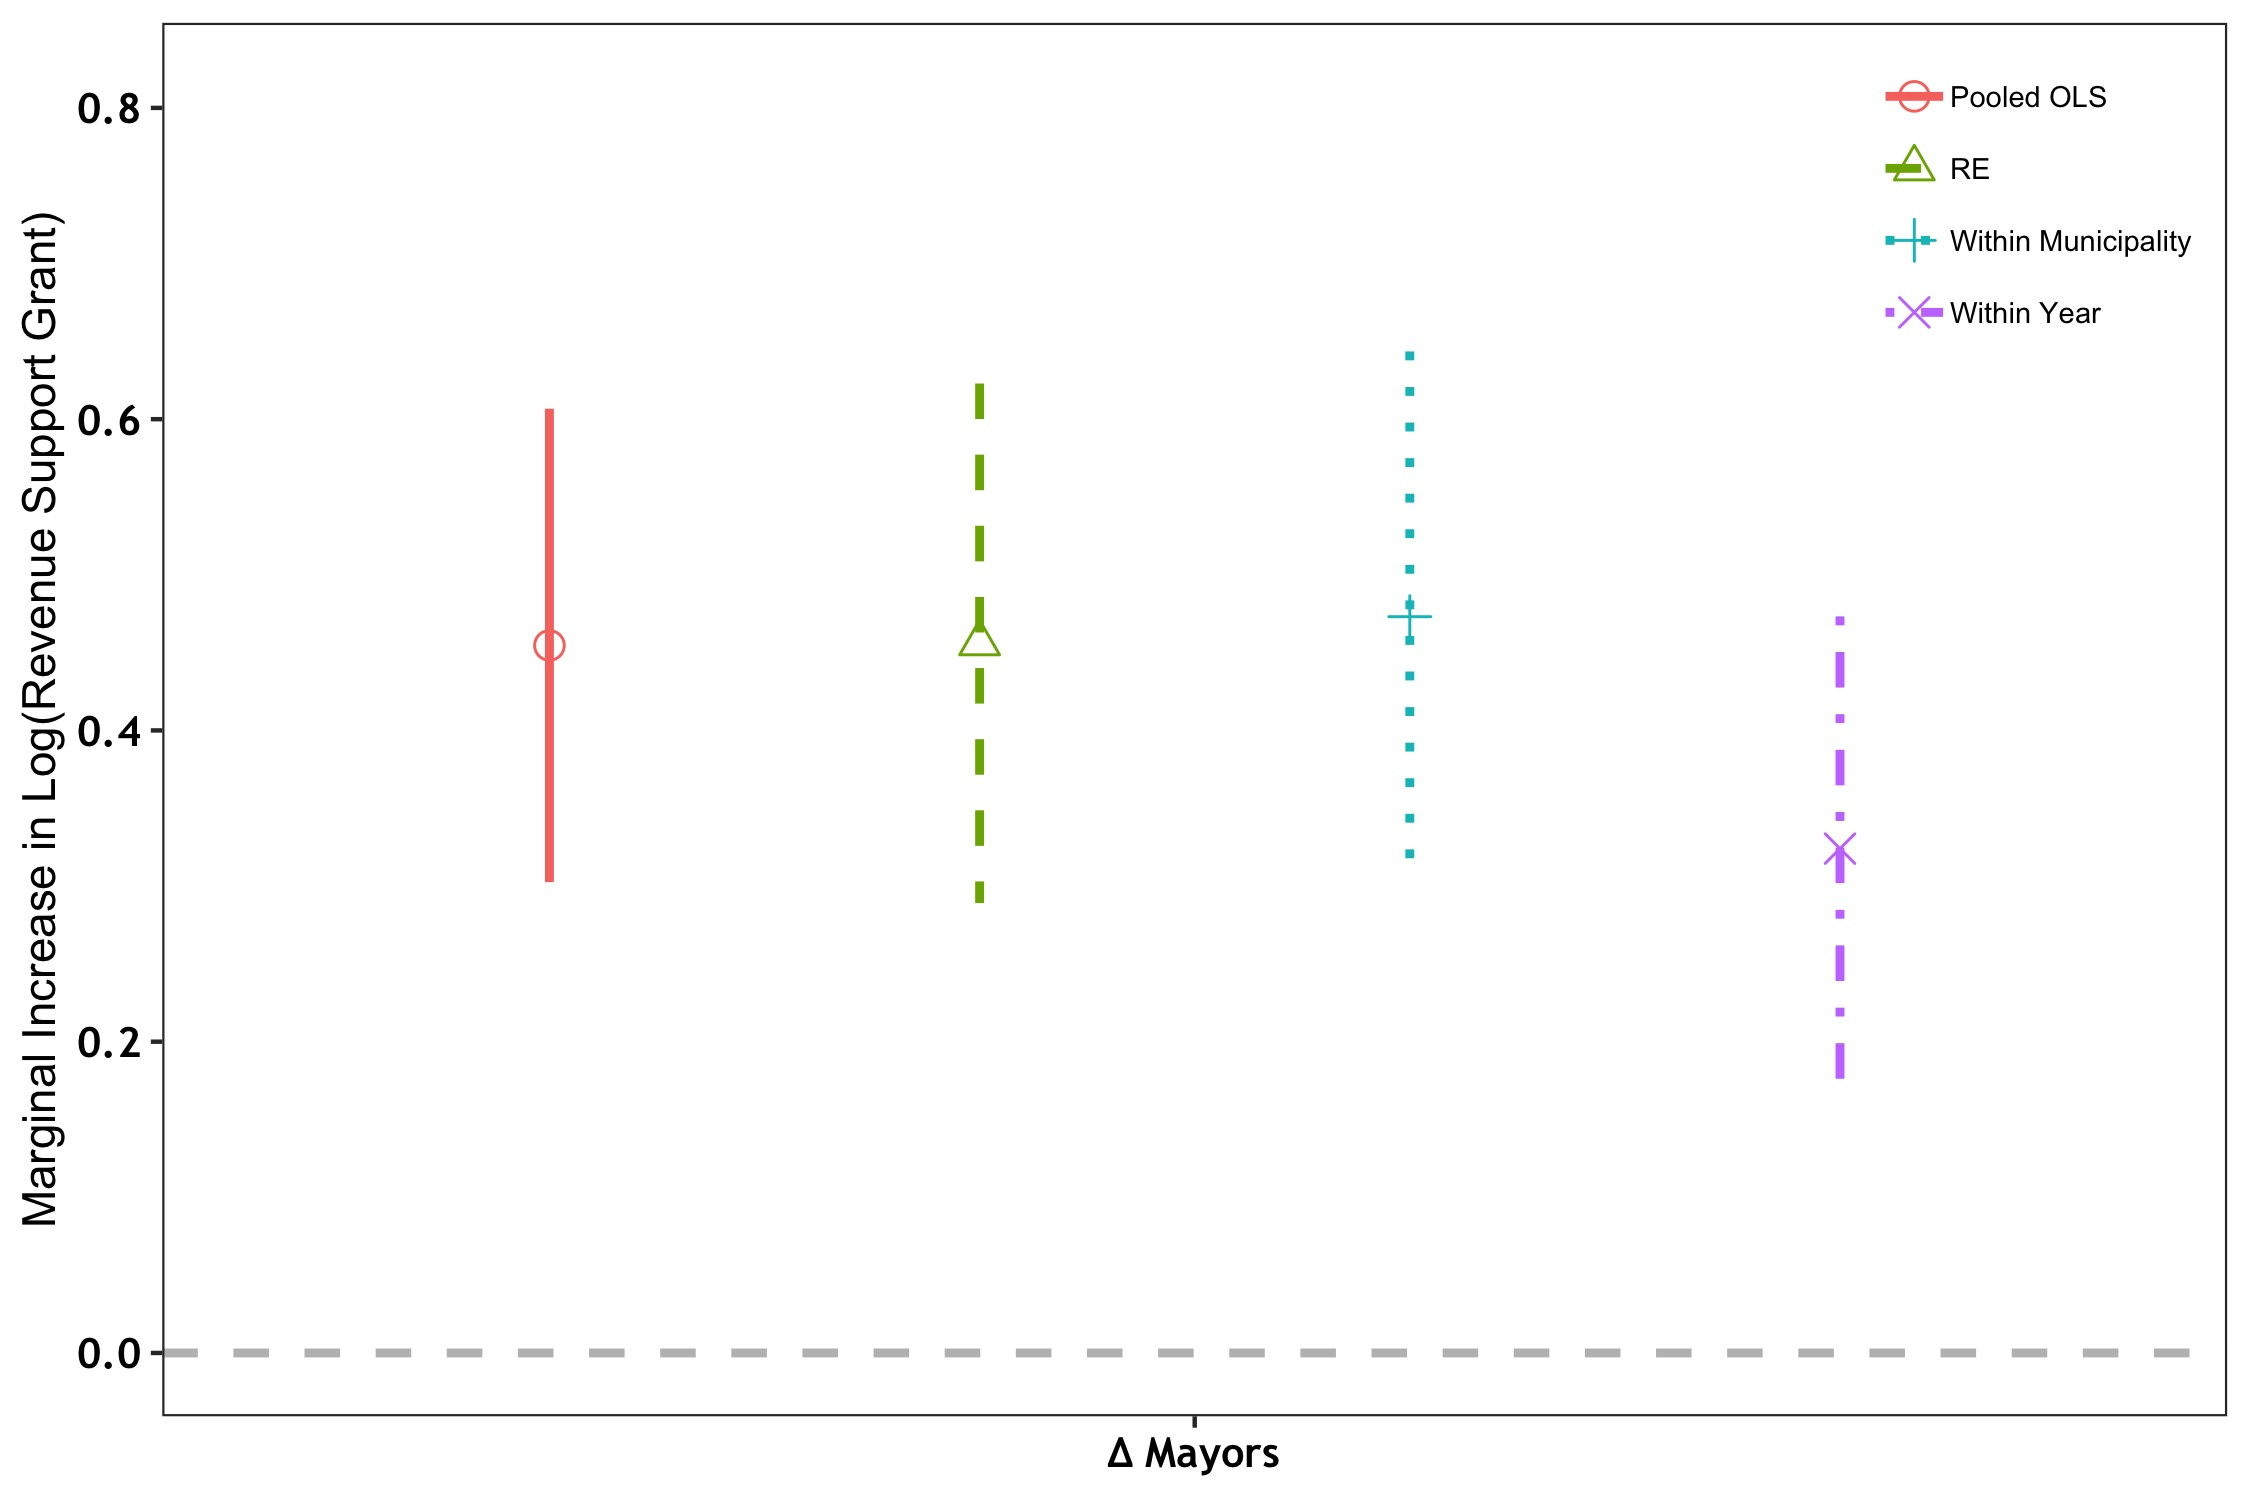
\includegraphics[width=7.2cm, height=6.5cm]{04-Chapter-Four/image/figure7-coef-table1.jpeg}
    \caption{The Variable of Interest in Table \ref{tab:table1}}
    \label{fig:margin-1}    
    \end{subfigure}    
    \begin{subfigure}[t]{0.45\textwidth}
    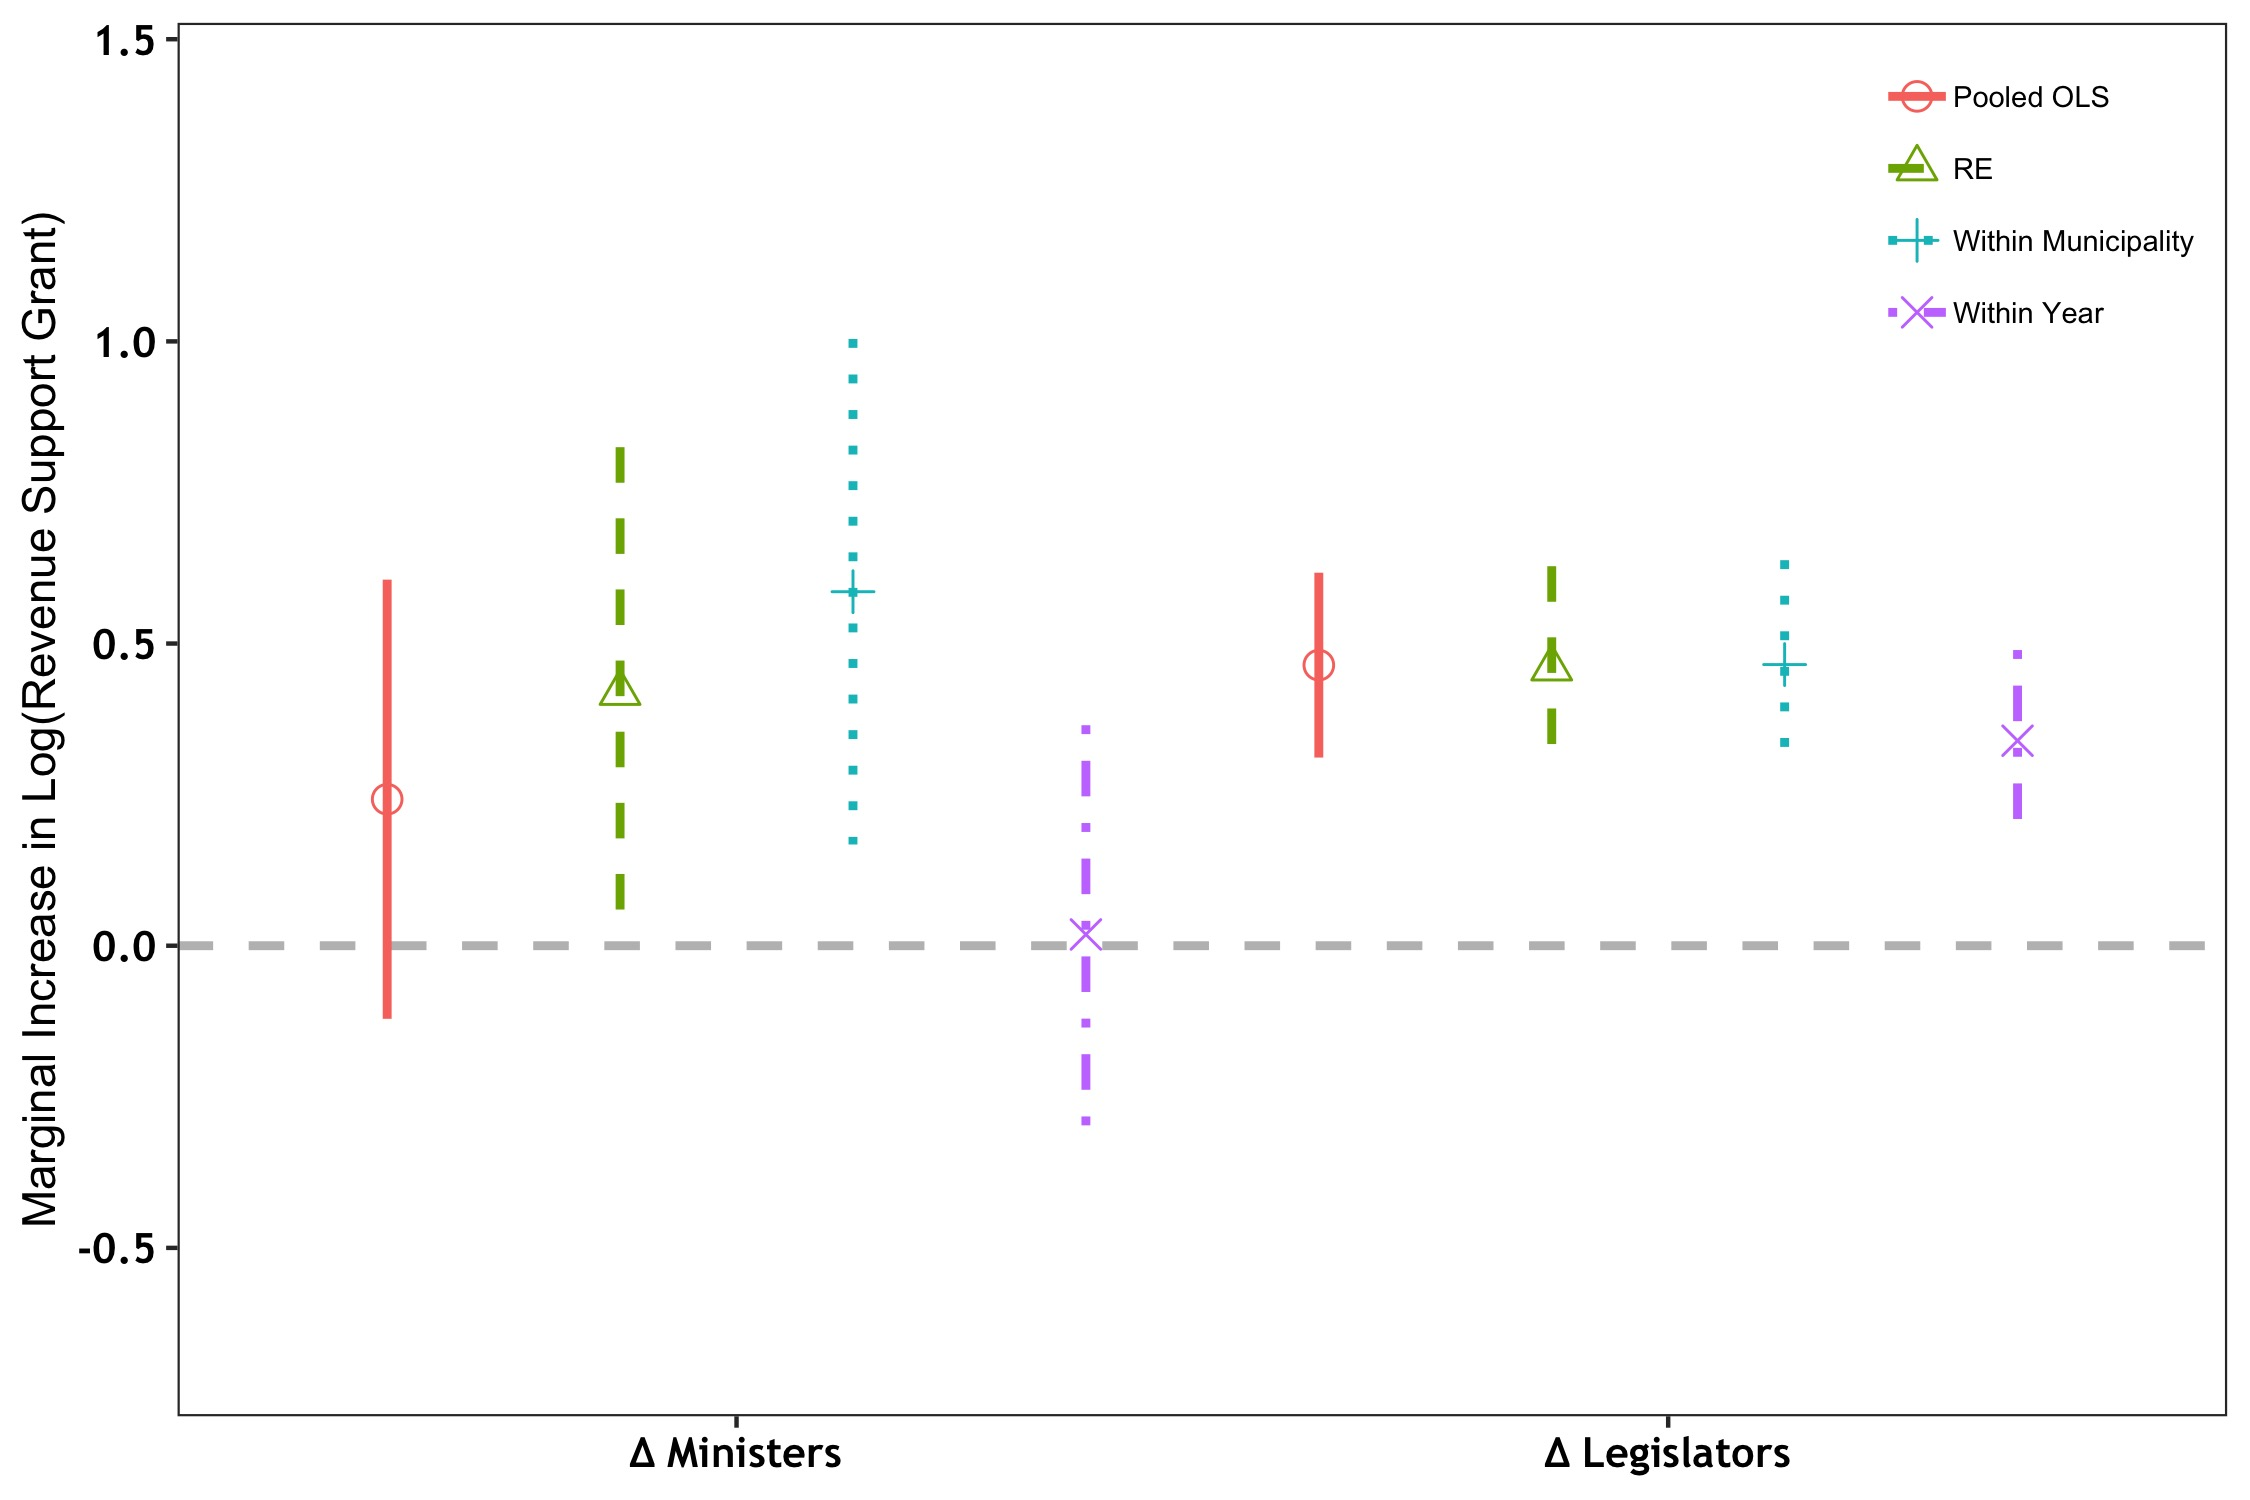
\includegraphics[width=7.2cm, height=6.5cm]{04-Chapter-Four/image/figure7-coef-table2.jpeg}
    \caption{The Variable of Interest in Table \ref{tab:table2}} 
    \label{fig:margin-2}
    \end{subfigure}
    \raggedright
    \begin{subfigure}[t]{0.45\textwidth}
    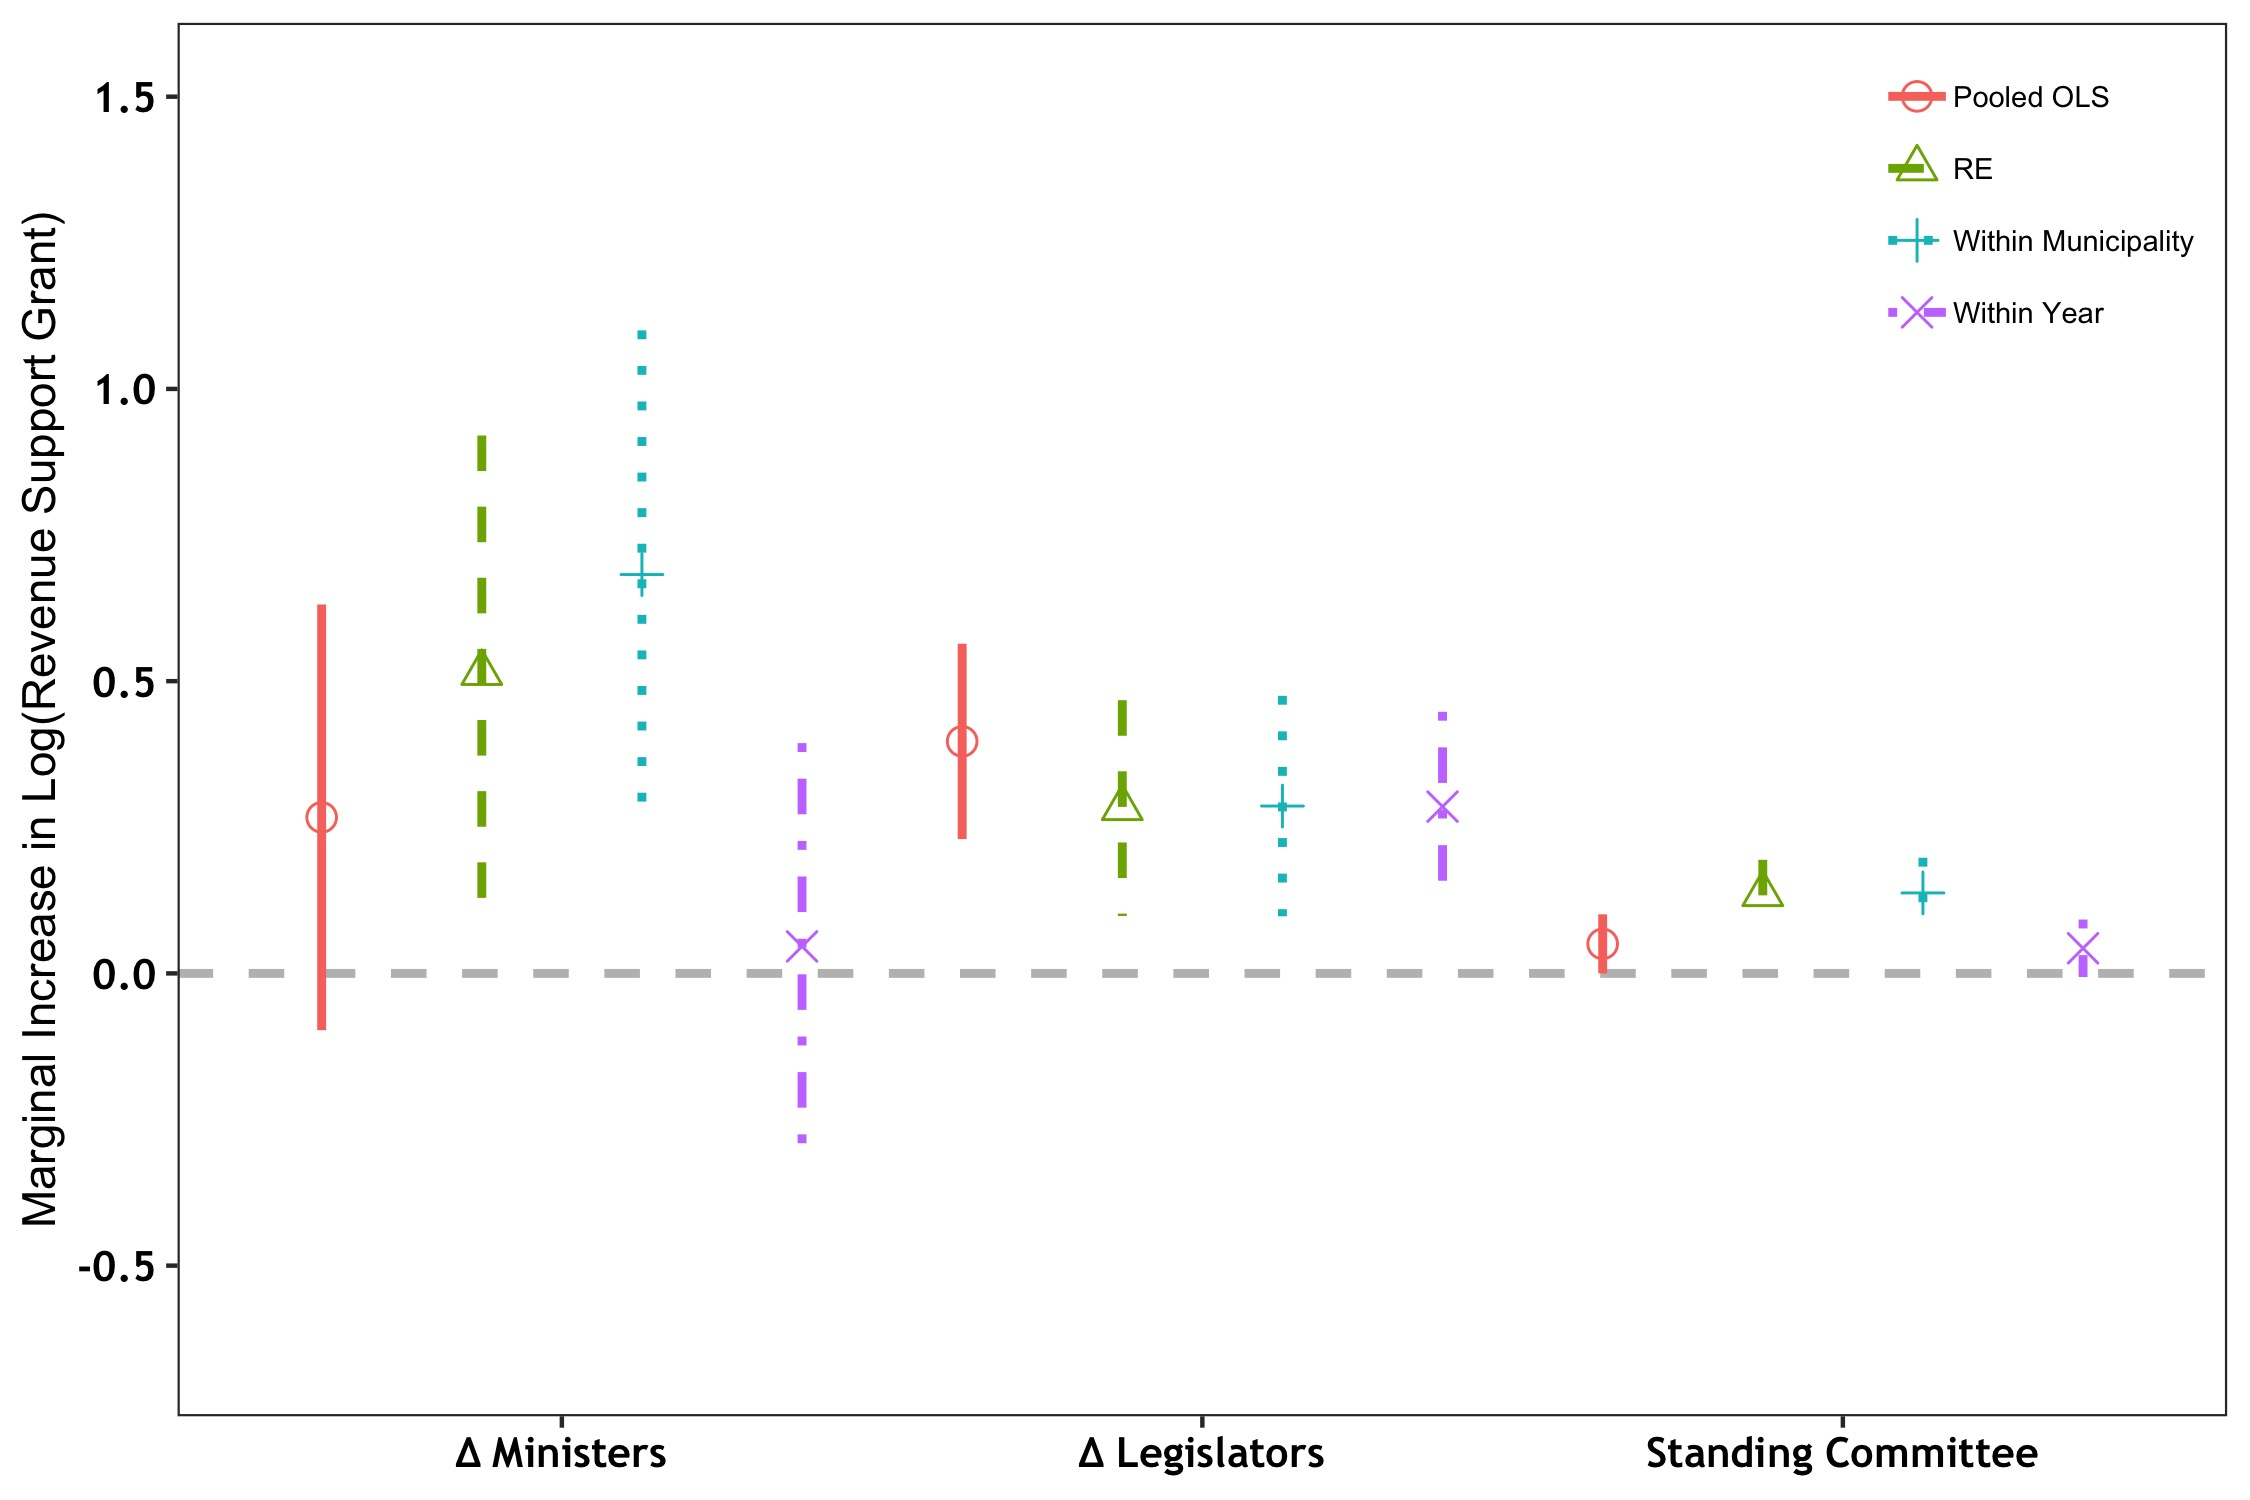
\includegraphics[width=7.2cm, height=6.5cm]{04-Chapter-Four/image/figure7-coef-table3.jpeg}
    \caption{The Variable of Interest in Table \ref{tab:table3}} 
    \label{fig:margin-3}
    \end{subfigure}    
    \caption{The Mayor\textquoteright s Years of Experience and Changes on the Marginal Increase in Revenue Support Grant by Regression Models\label{figure7}}
    \label{fig:margin-model}    
\end{figure}





%%%%%%%%%%%%%%%%%%%%%%%%%%%%%%%%%%%%%%%%%%%%%%%%%%%%%%%%%%%%
%%                         CV Page                        %% 
%%%%%%%%%%%%%%%%%%%%%%%%%%%%%%%%%%%%%%%%%%%%%%%%%%%%%%%%%%%%

% \begin{curriculumvitae}
%   Previous degrees and experience.
% \end{curriculumvitae}

\end{document}



